% =================================================================
% Tesi di laurea magistrale — Università di Siena, DIISM
% Ingegneria Informatica e dell'Informazione
%
% NOTA SUL FORMATO
% Il DIISM non pubblica specifiche tipografiche vincolanti (margini,
% carattere, interlinea): le linee guida di dipartimento riguardano
% la procedura, le scadenze e la lingua. L'unico elemento con un
% formato atteso e' il frontespizio. I valori qui sotto sono quindi
% una scelta consapevole, non un obbligo — ma sono coerenti fra loro,
% che e' cio' che il preambolo precedente non era.
% =================================================================
\documentclass[12pt,a4paper,oneside]{report}

% ---------------------------------------------------------------
% CODIFICA E LINGUA
% Un solo inputenc. Il preambolo precedente ne caricava due con
% codifiche opposte (utf8 e poi latin1) e vinceva il secondo: su file
% salvati in UTF-8 -- come sono tutti i .tex di questa tesi, verificato
% -- i circa 3.500 caratteri accentati risultavano corrotti.
% ---------------------------------------------------------------
\usepackage[utf8]{inputenc}
\usepackage[T1]{fontenc}
\usepackage{lmodern}          % font vettoriale: niente bitmap nel PDF
\usepackage[british]{babel}
\usepackage{microtype}        % giustificazione piu' uniforme

% ---------------------------------------------------------------
% LAYOUT DI PAGINA
% Un solo posto in cui e' definito. Il preambolo precedente fissava i
% margini con geometry e poi li riscriveva a mano con \oddsidemargin,
% \textheight e \topmargin: il risultato effettivo era 4,02 cm a
% sinistra contro 2,98 a destra, e 3,54 cm sopra contro 3,66 sotto,
% non i 3,5 e i 2 che geometry dichiarava.
%
% Sinistra > destra e' voluto: il documento e' oneside e va rilegato.
% ---------------------------------------------------------------
\usepackage{geometry}
\geometry{a4paper,
          top=3cm, bottom=3cm, left=3.5cm, right=3cm,
          headheight=15pt, headsep=1cm, footskip=1.2cm}

% ---------------------------------------------------------------
% INTERLINEA
% \onehalfspacing di setspace corrisponde all'interlinea 1,5 di Word.
% Il valore precedente era ambiguo: \baselinestretch{1.5} veniva
% annullato da \linespread{1.3} venti righe dopo, quindi l'interlinea
% reale era 1,3. Scrivere \linespread{1.5} sarebbe comunque troppo:
% darebbe 21,8 pt su un corpo di 12, cioe' 1,8 volte il corpo.
% ---------------------------------------------------------------
\usepackage{setspace}
\onehalfspacing

% Paragrafi allineati al margine, senza rientro, separati da uno spazio
% bianco. E' una scelta, non un difetto: NON caricare indentfirst
% insieme a questo, perche' i due si annullano a vicenda.
\usepackage{parskip}

% ---------------------------------------------------------------
% TESTATA DEI CAPITOLI
% La classe report lascia 50 pt di bianco sopra il numero del capitolo
% e altri 40 sotto il titolo: il testo comincia a circa un terzo della
% pagina. Qui il bianco sopra scende a 10 pt, cioe' il titolo si alza
% di circa 1,4 cm, e quello sotto a 30 pt.
%
% La forma del titolo non cambia: si tocca solo la spaziatura. Per
% alzarlo ancora, ridurre il primo \vspace* (anche a 0 pt); per
% abbassarlo, aumentarlo verso i 50 pt originali.
% ---------------------------------------------------------------
% \AtBeginDocument: la redefinizione viene applicata all'apertura del
% documento, quindi vale anche se un pacchetto caricato piu' sotto
% ridefinisse a sua volta la testata. Senza, l'ordine conta.
\makeatletter
\AtBeginDocument{%
\renewcommand{\@makechapterhead}[1]{%
  \vspace*{-20\p@}%
  {\parindent \z@ \raggedright \normalfont
    \ifnum \c@secnumdepth >\m@ne
      \huge\bfseries \@chapapp\space \thechapter
      \par\nobreak
      \vskip 12\p@
    \fi
    \interlinepenalty\@M
    \Huge \bfseries #1\par\nobreak
    \vskip 30\p@
  }}
% Stessa cosa per i capitoli non numerati: Introduzione, Ringraziamenti,
% Bibliografia. Senza questa seconda definizione resterebbero in basso.
\renewcommand{\@makeschapterhead}[1]{%
  \vspace*{-20\p@}%
  {\parindent \z@ \raggedright \normalfont
    \interlinepenalty\@M
    \Huge \bfseries #1\par\nobreak
    \vskip 30\p@
  }}
}
\makeatother

% ---------------------------------------------------------------
% INTESTAZIONI
% Sintassi fancyhdr moderna. Quella precedente (\rhead[..]{..} con
% \fancyplain) e' della versione 1 del pacchetto, deprecata da anni.
% Soprattutto: la configurazione era inerte, perche' nel corpo del
% documento un \pagestyle{myheadings} la sostituiva prima del primo
% capitolo.
% ---------------------------------------------------------------
\usepackage{fancyhdr}
\pagestyle{fancy}
\fancyhf{}
\renewcommand{\chaptermark}[1]{\markboth{\thechapter.\ #1}{}}
\renewcommand{\sectionmark}[1]{\markright{\thesection\ #1}{}}
\fancyhead[L]{\bfseries\nouppercase{\leftmark}}
\fancyhead[R]{\bfseries\thepage}
\renewcommand{\headrulewidth}{0.4pt}

% Prima pagina di ogni capitolo: solo il numero, in basso
\fancypagestyle{plain}{%
  \fancyhf{}\fancyfoot[C]{\thepage}%
  \renewcommand{\headrulewidth}{0pt}}

% ---------------------------------------------------------------
% MATEMATICA
% ---------------------------------------------------------------
\usepackage{amsmath}
\usepackage{amssymb}
\usepackage{amsfonts}
\usepackage{amsthm}
\usepackage{mathtools}
\usepackage{bm}

% ---------------------------------------------------------------
% FIGURE E TABELLE
% subfig e' stato tolto: non e' usato in nessun capitolo (zero
% \subfloat) ed entra in conflitto con caption e hyperref. Se
% servissero sottofigure, il pacchetto da caricare e' subcaption.
% ---------------------------------------------------------------
\usepackage{graphicx}
\graphicspath{{figure/}}
\usepackage{booktabs}     % \toprule \midrule \bottomrule
\usepackage{multirow}
\usepackage{adjustbox}
\usepackage{placeins}
\usepackage{caption}
\captionsetup{font=small, labelfont=bf, width=.92\textwidth}

% Cifre decimali con la virgola, come da uso italiano
\usepackage{siunitx}
\sisetup{output-decimal-marker={,}, group-separator={.},
         group-minimum-digits=4}

% ---------------------------------------------------------------
% CODICE
% ---------------------------------------------------------------
\usepackage{xcolor}
\usepackage{listings}
\lstset{basicstyle=\ttfamily\small,
  showstringspaces=false,
  commentstyle=\color{red},
  keywordstyle=\color{blue},
  breaklines=true,
  escapeinside={(*@}{@*)}
}

% ---------------------------------------------------------------
% RIFERIMENTI INCROCIATI
% La tesi contiene 101 \ref e 38 \cite: senza hyperref il PDF non e'
% navigabile. Va caricato per ultimo, dopo tutto il resto.
% hidelinks toglie i riquadri colorati, che in stampa sono un difetto.
% ---------------------------------------------------------------
\usepackage[hidelinks]{hyperref}
\hypersetup{
  pdftitle={Evaluation of a Pose-Based Fall Detection System: From Controlled Environments to Real-World Edge Deployment},
  pdfauthor={Caterina Cerretani},
  bookmarksnumbered=true,
  linktoc=all
}

% ---------------------------------------------------------------
% AMBIENTI E ABBREVIAZIONI
% ---------------------------------------------------------------
\newtheorem{Thm}{Theorem}[section]
\newtheorem{Lem}[Thm]{Lemma}
\newtheorem{Prop}[Thm]{Proposition}
\newtheorem{Cor}[Thm]{Corollary}
\newtheorem{Exer}[Thm]{Exercise}
\newtheorem{Def}[Thm]{Definition}
\newtheorem{Conj}[Thm]{Conjecture}
\newtheorem{ST}[Thm]{Terminal State}
\newtheorem{Ques}{Question}[chapter]
\newtheorem{Rmk}[Thm]{Remark}

\theoremstyle{definition}
\newtheorem{Ex}{Example}[section]
\newtheorem{Oss}[Thm]{Observation}
\newtheorem{Not}[Thm]{Notation}

\newcommand{\RR}{{\mathbb{R}}}
\newcommand{\ZZ}{{\mathbb{Z}}}
\newcommand{\NN}{{\mathbb{N}}}
\newcommand{\HH}{{\mathcal{H}}}
\newcommand{\MM}{{\mathcal{M}}}
\newcommand{\VV}{{\mathcal{V}}}
\newcommand{\PP}{{\mathbb{P}}}
\newcommand{\FF}{{\mathcal{F}}}
\newcommand{\CC}{{\mathcal{C}}}
\newcommand{\PPP}{{\mathbb{P}}}
\newcommand{\CCC}{{\mathbb{C}}}
\newcommand{\BB}{{\mathcal B}}

\def\cA{\mathcal A}
\def\cR{\mathcal R}
\def\cG{\mathcal G}
\def\cT{\mathcal T}

\newcommand{\bx}{{\mathbf x}}
\newcommand{\by}{{\mathbf y}}
\newcommand{\bp}{{\mathbf p}}
\newcommand{\bq}{{\mathbf q}}
\newcommand{\bb}{{\mathbf b}}
\newcommand{\bc}{{\mathbf c}}
\newcommand{\ba}{{\mathbf a}}
\newcommand{\bv}{{\mathbf v}}
\newcommand{\bt}{{\mathbf t}}

\hyphenation{re-pre-sen-ta-tion}
\hyphenation{ge-ne-ra-li-sa-tion}

% =================================================================
\begin{document}

\pagestyle{empty}
\newgeometry{top=12mm,bottom=15mm,inner=25mm,outer=25mm}

\begin{titlepage}
\begin{spacing}{1.4}

\begin{figure}[ht]
\centering

\includegraphics[height=65mm]{LOGO_UNISI_VERTICALE_NERO_0.pdf}
\end{figure}

\begin{center}

{\scshape \Large
Department of\\
Information Engineering and Mathematics
}

\vspace{-2mm}

\rule[0.1cm]{140mm}{0.1mm}
\rule[0.5cm]{140mm}{0.6mm}

\vspace{-2mm}

{\large
M. Sc. Program\\
ARTIFICIAL INTELLIGENCE AND AUTOMATION ENGINEERING
}

\vspace{20mm}

\begin{spacing}{1.8}
{\huge \bf
Evaluation of a Pose-Based Fall Detection System: From Controlled Environments to Real-World Edge Deployment
}
\end{spacing}

\end{center}

\vspace{8mm}
\noindent
\begin{minipage}[t]{0.5\textwidth}
\bf
Supervisor:\\
Prof. Alessandro Mecocci
\end{minipage}
\hfill
\begin{minipage}[t]{0.5\textwidth}
\raggedleft
\bf
Candidate:\\
Caterina Cerretani
\end{minipage}

\vfill

\begin{center}
\large
\bf
Academic Year 2025-2026
\end{center}

\end{spacing}
\end{titlepage}

\restoregeometry

\cleardoublepage
\pagestyle{plain}
\pagenumbering{roman}
\tableofcontents
\listoffigures
\listoftables

% ---------------------------------------------------------------
% Da qui in poi numerazione araba e intestazioni correnti.
% L'Introduzione entra nel corpo: nel preambolo precedente restava
% nella numerazione romana insieme all'indice.
% ---------------------------------------------------------------
\cleardoublepage
\pagenumbering{arabic}
\pagestyle{fancy}

\chapter*{Introduction}
\addcontentsline{toc}{chapter}{Introduction}
\setcounter{chapter}{0}

In recent years, automatic fall detection has become an important research topic in Ambient Assisted Living because falls may have severe consequences, particularly for older adults. Interest has consequently grown in monitoring systems that can be used within healthcare and care
facilities and in domestic environments.

The problem nevertheless remains complex, because some daily activities, such
as sitting down or bending over, may appear visually similar to a fall.
For this reason it is not sufficient to consider only the person's final
posture, but also the way in which that posture is reached. It therefore
becomes important to describe the temporal evolution of the body, taking into
account information such as changes in orientation, velocity, relative
displacements of the different anatomical parts and other quantities related
to the dynamics of the movement.

The objective of this thesis is to analyse and verify the possibility of
detecting a fall and distinguishing it from a normal daily activity by means
of a system based on \emph{pose estimation} with the aim of enabling earlier detection, supporting timely assistance and reducing the need to transmit identifiable visual information.

Most existing studies report classifier performance on controlled datasets. However, these results do not necessarily indicate how the complete system behaves when the subject, viewpoint, acquisition domain and computational platform change. This thesis therefore investigates both the relative role of movement representation and classifier architecture, and the progressive
degradation or preservation of performance when the system is moved towards realistic operating conditions.

In more detail, the thesis is divided as follows. Chapter \ref{cap:contesto}
provides an introduction to the field of automatic fall detection, focusing on
the importance of the problem in the older population and on the consequences
a fall entails, on the main requirements a system must satisfy in order to be
genuinely installable, and on the difficulties that arise when it has to
operate in a real environment.
Chapter \ref{cap:stato_arte} reviews the main concepts of fall detection
proposed in the literature, such as the different technologies employed, the
representations of human movement, the models used for temporal
classification and the problems related to datasets and evaluation protocols.
Chapter \ref{cap:metodologia} describes the methodology adopted, following the
path that leads from pose estimation to the final decision. It presents the
geometric representations considered, the construction of the temporal
features, their analysis and selection, and the formation of the sequences
used by the classifiers.
Chapter \ref{cap:protocollo} defines the protocol used for the evaluation and
presents the main experimental results. After class imbalance, subject-wise
partitioning, normalisation and the choice of the decision threshold, the
chapter compares the different representations and architectures and studies
the effect of the viewpoint, the definition of the task and the transfer to an
external dataset.
Finally, Chapter \ref{cap:edge} analyses the implementation of the entire
pipeline on an \emph{edge} device and its validation under conditions closer
to those of real use. It examines in depth the computational cost of the
individual stages, the behaviour of the system on the device and the results
obtained during the sessions recorded in domestic environments, moving from
the individual predictions of the classifier to the alarm events produced
during continuous operation.
Chapter 
ef{cap:discussion} discusses the results obtained as a whole, relating the individual experiments to one another in order to identify which factors most affect the behaviour of the system, and draws the conclusions of the work together with the limitations of the evaluation.


\chapter{Application context and problem formulation}
\label{cap:contesto}

Italy is today the oldest country in Europe and the second
oldest in the world after Japan. As the average age rises, the demand for
care grows accordingly. This demographic trend increases the demand for care services at a time when the availability of nursing personnel is already limited. The ratio of nursing staff to population remains below the European average, and between 2026 and 2035 about eighty thousand retirements are expected among that staff \cite{FN}.
Among the events that make such care necessary, falls represent one of the
most significant problems for the older population. A fall may cause severe
physical consequences, require a period of rehabilitation and, in the most
serious cases, compromise a person's independence.

The consequences concern not only the health of the individual, but also the
care and economic burden that follows from it. In hospitals and in
residential care facilities (RSA), a fall may lead to days of
hospitalisation, to a rehabilitation pathway and to a need for staff, whose availability is already limited. In the domestic environment the burden
falls instead mainly on families. In Italy about 1,1 million people provide
non-professional care, often bearing the associated costs directly as well
\cite{FN}.
The problem becomes more relevant when the event is not directly monitored.
An older person living alone may be unable to get up or to ask for
assistance independently, remaining on the ground for a prolonged period
before help is provided.

It is in this scenario that \emph{fall detection} systems come into play, designed
to monitor a person's behaviour continuously, to recognise a possible fall
promptly and to generate an alarm signal. Automatic fall detection is
therefore one of the problems that the field of \emph{Ambient Assisted
Living} (AAL) seeks to address and to solve, with technologies developed to
support the safety and the independence of people in their everyday
environments.
We shall use this first chapter to provide a brief introduction to the
context in which a detection system has to operate. In particular, we shall
focus our attention on the relevance of falls in the older population and in
the domestic environment; we shall identify the main requirements that an
automatic detection system should satisfy; and finally we shall analyse the
difficulties that arise when moving from controlled data to a real
environment.

\section{Ambient Assisted Living and the clinical relevance of falls}

The progressive ageing of the population increases the need for solutions
capable of supporting the monitoring and the care of older people, both in
the domestic environment and in care contexts such as hospitals and
residential care facilities (RSA).

As of 1 January 2026, according to the ISTAT Annual Report, people aged 65 or
over represent 25,1\% of the Italian population, having increased by 11,3\%
over the course of a decade, while over the same period the population up to
14 years of age has decreased (Figure~\ref{fig:popolazione}) \cite{IS}. This
is therefore a numerically significant group, destined to weigh ever more
heavily on health, care and home-assistance services.

Within this age group, falls represent a critical event both for their
frequency and for their consequences on the health and the independence of
the person. According to the \emph{PASSI d'Argento} surveillance programme of
the Italian National Institute of Health, the data for the two-year period
2023-2024 indicate that about one older adult in five reports at least one fall
in the preceding twelve months. The frequency increases appreciably with age,
rising from 15\% in the band between 65 and 74 years to 31\% beyond the age
of 85, and is higher among women, with a percentage of 24\% compared with the
15\% observed among men \cite{PA}.

\begin{figure}[htbp]
    \centering
    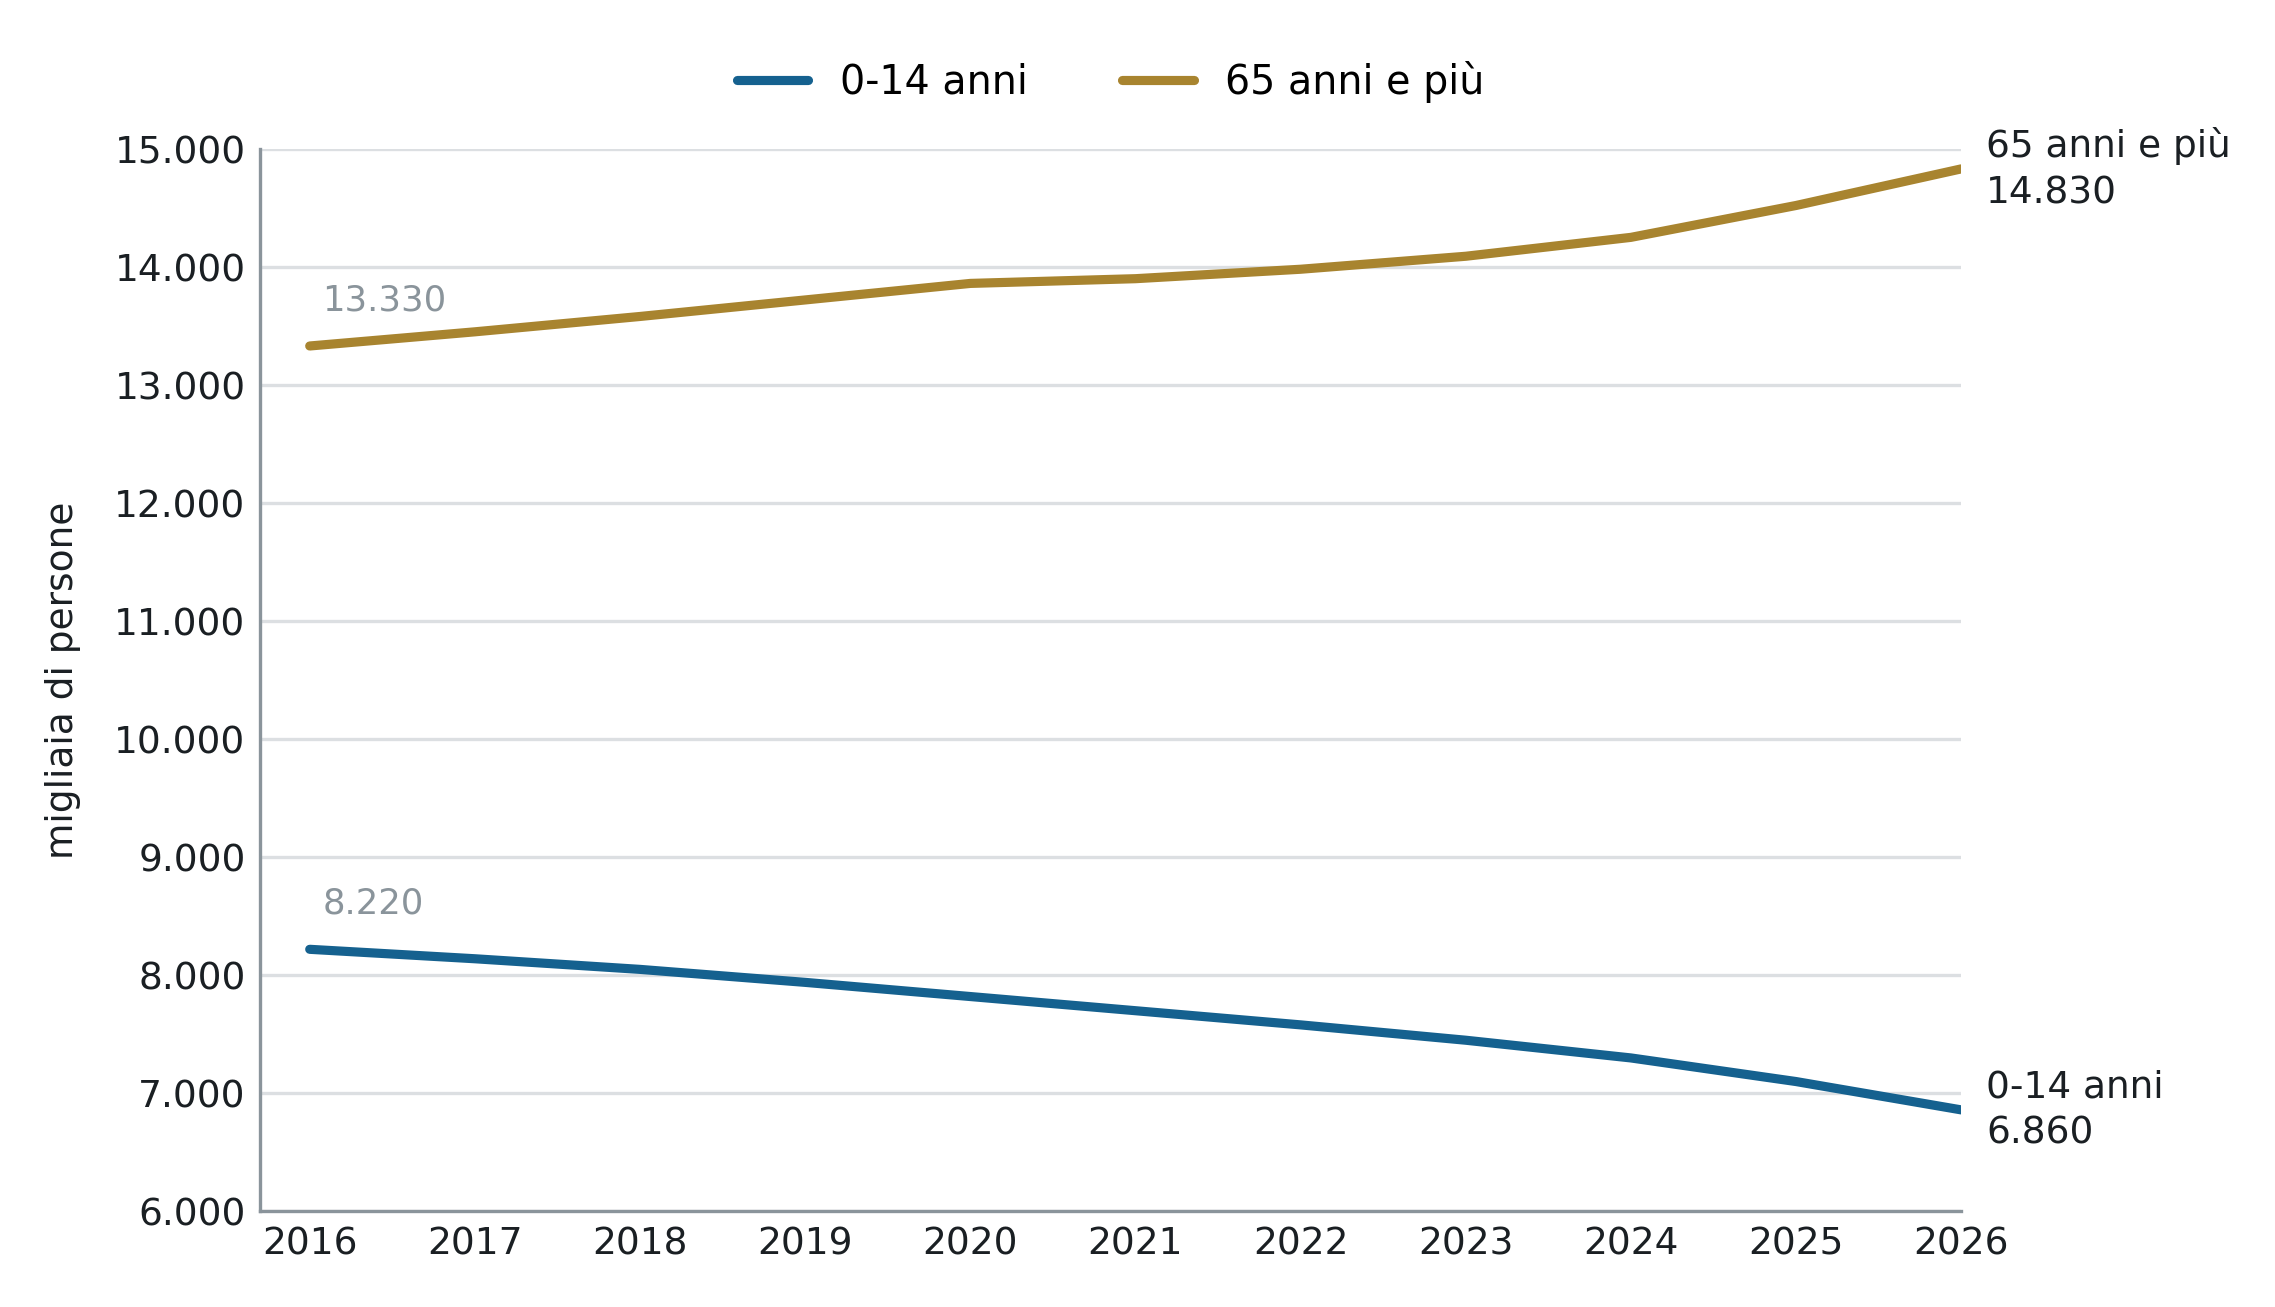
\includegraphics[width=0.85\linewidth]{figure/fig_popolazione.png}
    \caption{Italian population in the age bands 0-14 and 65 years and over,
    2016-2026.}
    \label{fig:popolazione}
\end{figure}

\subsection{Falls in the domestic environment and consequences for the person}

In a fall detection system it is not sufficient to know how often a person
falls; it is also necessary to consider where the event takes place and how
quickly it can be detected. Falls among people over sixty-five occur predominantly in the domestic environment: about 54\% take place at home, against 21\% in the garden, 20\% in the street and the remaining 5\% elsewhere \cite{PA}.

Falls are frequent in hospitals and care facilities as well. In that context,
however, the presence of staff generally makes it more likely that the event
is observed and that help arrives quickly. At home, by contrast, that
supervision is absent: the older person may remain on the ground for a much
longer time before anyone notices the fall, and particularly so if they live
alone.
The value of automatic detection is therefore greatest where human
supervision is absent. This does not rule out use in hospitals or in
residential care facilities, since a system of this kind remains useful for
reducing intervention times; but it explains why the domestic case is the one
on which the present work concentrates, and where it was experimentally
validated.

It is important to stress that the consequences of a fall do not depend on
the initial traumatic event alone. As reported in \cite{PA}, about 18\% of
falls caused a fracture and 16\% of falls required a hospital stay of at least
one day. Among hospital admissions for domestic accidents in the older
population, the most frequent diagnosis is hip fracture. Moreover, there
remains the problem of lying on the ground, which can favour secondary
complications such as dehydration, hypothermia, muscle damage and a general
worsening of the clinical condition.

Falls may also have psychological and functional consequences, including fear of falling, reduced confidence and the voluntary restriction of normal daily activities. Reducing the time between the fall and the arrival of help therefore does not serve only to limit the immediate damage: it is essential in order to guarantee a sustainable life in one's own home.

\section{Requirements of an automatic fall detection system}

A system intended for the detection of falls in a domestic or care
environment must satisfy requirements different from those of a classifier
evaluated exclusively on offline datasets. Achieving good classification
performance is not enough for the model to be usable.

For a solution of this kind to be adoptable, it must first of all detect the
event within a sufficiently short time and, at the same time, limit the
number of false alarms. A system that detects falls correctly but produces
continual alerts during normal daily activities risks becoming of little use
and, over time, being ignored or switched off. It must moreover handle data in a way compatible with the privacy of the people being monitored. Finally, the computational cost and that of the hardware must remain sufficiently contained to make a real installation and continuous operation possible.

These conditions translate into three main requirements: the first concerns
the operational reliability of the system and includes both the ability to
detect a fall promptly and the ability to contain false alarms. These two
aspects cannot be considered separately because improving one may entail the
worsening of the other. The second requirement concerns the protection of
privacy, while the third concerns the computational and economic
sustainability of the solution.

For these requirements to be experimentally verifiable, it is useful to translate them into measurable quantities. Table \ref{tab:criteri_valutazione} shows this correspondence, specifying the section in which each quantity is subsequently reported and verified.

\begin{table}[htbp]
\centering
\caption{Criteria used to evaluate the system.}
\label{tab:criteri_valutazione}
\resizebox{\textwidth}{!}{
\begin{tabular}{lll}
\toprule
\textbf{Requirement} & \textbf{Corresponding evaluation quantity} & \textbf{Section} \\
\midrule
Timeliness & Detection latency & \ref{sec:latenza} \\
Reliability & Event recall / missed falls & \ref{sec:recall-campo} \\
Alarm sustainability & False alarms per hour & \ref{sec:falsi-allarmi} \\
Computational feasibility & FPS / latency / memory / temperature & \ref{sec:costo-computazionale} \\
Privacy & Information retained, stored or transmitted & \ref{sec:protocollo-campo} \\
Continuous operation & Uninterrupted operating time & \ref{sec:continuita} \\
\bottomrule
\end{tabular}
}
\end{table}

\subsection{Timeliness and the sustainability of the alarm load}

The first requirement concerns timeliness. As discussed in the previous
section, a person who is unable to get up after a fall may remain on the
ground for a prolonged period before receiving assistance. The system must
therefore be able to recognise the event and generate an alert within a
sufficiently short interval of time.

Timeliness cannot, however, be considered separately from the reliability of
the alarm. A continuously active system produces a large number of decisions,
and every false positive may require a check by a family member, by a
caregiver or by care staff. If these alerts become too frequent, the system
risks proving of little use in everyday operation, even when it manages to
recognise most falls correctly.

Therefore, in real applications the number of false alarms produced per unit
of time takes on particular importance. One of the quantitative figures
available in the literature comes from a study conducted on sixteen older
adults monitored by means of a worn accelerometer, over a total of about
15.500 hours of use, reporting a rate of \textbf{0,049 alarms per hour}
\cite{KA}.
However, this value cannot be compared with the one produced by a vision-based system, since the acquisition modalities and the possible causes of error are different. The figure can nonetheless be used above all as a reference for the order of magnitude.

It is important to distinguish between two levels of evaluation. The first focuses on individual time windows and analyses the behaviour of the classifier. The second, on the other hand, concerns the alarm events that the system generates during operation. Several consecutive positive windows may belong to the same episode and can therefore be grouped into a single alarm. For this reason, the false positive rate per window and the number of false alarms per hour represent two different aspects of the system. The former measures the errors produced in individual windows, whilst the latter indicates how many false alarms are actually generated over time.

Precisely because the evaluation of vision-based systems is carried out
predominantly on laboratory datasets, classification metrics alone, such as
precision, recall and F-score, are not sufficient. The behaviour of the system
during prolonged operation is therefore also considered, distinguishing the
performance of the classifier on the individual temporal windows from the
number of alarm events actually generated.

\subsection{Confidentiality and local processing}

The use of a camera inside a home introduces a second important requirement:
the protection of personal data. An ordinary RGB stream may contain
identifying information relating to the person, to the environment in which
they live and to the activities they are performing.

The system should therefore minimise the use, storage and transmission of such identifiable visual information, using the original images only when necessary. However, this does not automatically guarantee the anonymity of the data, as even representations derived from the person's pose or movement may retain individual characteristics.

This choice reduces both the amount of identifiable visual information available to subsequent stages and the dimensionality of the data supplied to the classifier. Processing is moreover kept locally on the device, so that the video stream need not be transmitted to an external server. Only the data necessary for handling a possible alarm are sent outside.
This requirement motivates the pose-based, locally processed architecture developed in Chapter \ref{cap:metodologia}. 

\subsection{Cost, resources and edge architecture}

The choice to perform processing locally imposes a constraint on the available computational resources. A system intended to be installed permanently in a home or in a care facility should be able to run on compact, low-cost hardware, without necessarily depending on a workstation or on a remote computing infrastructure. Feasibility on the \emph{edge} device does not depend on the classifier alone. 

The computational cost should be assessed by considering data acquisition, pose estimation, feature extraction and classification together. 
It is thus necessary to strike a balance between recognition capability, computational complexity, latency and the ability to keep the entire pipeline running over time. This requirement leads to the adoption of an \emph{edge} architecture, the computational feasibility of which is verified experimentally in Chapter \ref{cap:edge}.

\section{Critical issues in the transfer from controlled data to the real
environment}

Evaluation on a controlled dataset makes it possible to compare
representations and models reproducibly, but it does not guarantee that the
system will maintain the same behaviour once installed in a real environment.

During the collection of a dataset many conditions are known or
controlled: the position of the cameras, the activities performed by the
subjects, the duration of the recordings and, in general, the context in which
acquisition takes place. In a real home these conditions may instead vary over
time.
In the case of a system based on pose estimation, three aspects prove
particularly important:
\begin{enumerate}
    \item the change of domain and of recording geometry,
    \item the presence of occlusions,
    \item the different frequency with which a fall occurs compared with
          normal daily activities.
\end{enumerate}

\subsection{Domain variation and recording geometry}

A first critical issue is the change in acquisition conditions. The
representation obtained from the pose estimator depends not only on
the movement performed by the person, but also on the way in which this
movement is observed by the camera.

The same action may appear different when observed from the front, from the
side or from a more elevated position. As a consequence, quantities derived
from the landmarks as well, such as trunk inclination, the displacements of
the various parts of the body or their apparent velocities, may take on
different values while describing the same movement.
The viewpoint then becomes a real problem for a system installed in
environments different from the one in which the training data were collected.
To this are added other variations, such as lighting, distance from the
camera, background, frame rate and the physical characteristics of the
observed subjects. 


Taken together, these differences produce a \emph{domain shift}, that is, a variation in the distribution of the data with respect to the one used in training. This problem has been divided into five categories, each associated with a specific experimental test as shown in Table \ref{tab:domain_shift}.

\begin{table}[htbp]
\centering
\caption{Types of domain shift considered.}
\label{tab:domain_shift}

\begin{tabularx}{\textwidth}{l X c}
\toprule
\textbf{Category} &
\textbf{Change considered} &
\textbf{Section} \\
\midrule
\emph{subject domain}
& change the subject observed
& \ref{sec:loso} \\
\emph{viewpoint shift}
& change the position of the camera with respect to the person
& \ref{sec:viewpoint} \\
\emph{frame-rate shift}
& change the acquisition rate
& \ref{sec:framerate} \\
\emph{dataset shift}
& change the dataset used
& \ref{sec:domainshift} \\
\emph{environment shift}
& change the capture environment
& \ref{sec:campo} \\
\bottomrule
\end{tabularx}
\end{table}

The performance obtained on the source domain is not
sufficient, on its own, to describe the generalisation capability of the system. For this reason, the different forms of domain shift are evaluated separately in the subsequent experiments.

\subsection{Occlusions and the quality of pose estimation}

A second critical issue concerns the visibility of the body.
In datasets collected under controlled conditions the subject is generally
filmed so as to be clearly visible. In a domestic or care environment, by
contrast, the person may be partly hidden by beds, chairs, tables or other
items of furniture. Occlusion may moreover occur during a fall itself, when
the body changes configuration rapidly or approaches the floor.

Under such conditions, the pose estimator may supply unstable coordinates or
fail to localise some landmarks correctly.
The problem weighs more here than elsewhere, because the features used by the
classifier are built precisely from the coordinates of the skeleton. An error
in the estimate of a landmark may therefore propagate to the geometric and
temporal quantities computed in the subsequent stages.
In Chapter~\ref{cap:sperimentale} the sensitivity to a partial loss of
information is studied through controlled tests in which some groups of
landmarks are made temporarily unavailable.

\subsection{Event prevalence and the base rate of false alarms}

A last difference between an experimental dataset and real operation concerns
the \emph{prevalence of the positive class}, that is, the frequency with which falls actually occur.

A dataset useful for training must contain a sufficient number of positive
examples, and the resulting percentage of falls is much higher than the one a
system encounters in operation, where almost all observations belong to normal
daily activities. The imbalance changes the weight that has to be attributed to
false positives.
Even a false-positive probability of $10^{-3}$ per decision may become operationally relevant if the system
produces several decisions per second over many hours of continuous monitoring.

It is nevertheless necessary to distinguish between positive windows and
actual alarm events. Within the same episode, the classifier may produce several consecutive windows, which the system's logic returns as a single alert.
It then becomes useful to consider two levels of reading:
\begin{itemize}
    \item [-] The first concerns the individual temporal windows and describes
          the behaviour of the classifier;
    \item [-] the second concerns the alarm events produced during continuous
          operation.
\end{itemize}
In the second case the measure that matters is the number of false alarms per
unit of time, because it represents the burden that the system imposes on the
user, on family members or on care staff. Chapter \ref{cap:edge} measures the ratio between the two counts and compares it with what was observed in the two homes.

\section{Definition of the event to be recognised}

Another aspect that needs to be clarified concerns the definition of the event that the system must detect.
A fall does not correspond to a single posture, but to an event that unfolds over time. Generally, the person starts from a stable position, goes through a phase of loss of balance and rapid change in posture, and then ends up on the ground or at a lower level.

From this temporal sequence, three phases can therefore be distinguished: the phase preceding the fall, the transition phase occurring during the fall, and the subsequent phase in which the subject is on the ground.
From a classification perspective, this phenomenon can be described in three different ways. One can identify the \emph{fall event}, which is the dynamic phase during which the body loses its balance and moves rapidly downwards; one can also identify the \emph{post-fall state}, when the person is already on the ground; or both conditions can be considered to trigger an alarm.

These definitions are closely related, but they are not equivalent. A person may still be in a low or lying position even during normal daily activities. Actions such as sitting down, kneeling or lying down intentionally can produce configurations similar to those observed after a fall. Therefore, the final posture alone may not be sufficient to distinguish between the two cases, leading to the consideration of the dynamics through which that posture is achieved. A fall is generally associated with an involuntary and rapid change in body configuration, whilst a voluntary movement tends to unfold more gradually.
Defining the positive class therefore amounts to a choice regarding the task required of the classifier, rather than a mere convention used during data labelling; this is because altering what is considered positive means changing the classification problem and, consequently, the type of errors the system may produce.

This chapter clarifies what is considered positive, specifying which events the system must recognise: the fall phase, the subsequent state, or both. The operational rule by which this choice is then transformed into the labels of the time windows is illustrated in Section \ref{sec:compito}, which is dedicated to the creation of the windows.

\section{Research questions and objectives}

In light of the above considerations, the aim of this work is to develop and evaluate a \emph{fall detection} system based on human motion analysis and designed to run locally on a low-cost \emph{edge} device. Starting from an RGB video, the system derives a skeletal representation by estimating the person's pose and uses geometric and temporal information to recognise a fall.

Interest is not, however, focused solely on achieving good performance on the development dataset, but also on understanding which aspects of the pipeline actually influence the system's behaviour and to what extent the results obtained under controlled conditions hold true as usage conditions vary.
Based on these objectives, three research questions were formulated:
\begin{description}
    \item[RQ1.] When movement representation and evaluation protocol are fixed, how strongly does classifier architecture affect fall-detection performance?
    \item[RQ2.] How much of the performance obtained under controlled conditions is preserved when subject, viewpoint, dataset and acquisition environment change?
    \item[RQ3.] Can the complete pose-based detection pipeline operate continuously on a low-cost edge device while maintaining acceptable latency and alarm load?
\end{description}

To answer these questions, this study is structured around four main directions:
\begin{enumerate}
    \item \textbf{Movement representation}: building, starting from the
          skeletal landmarks, compact and interpretable geometric and temporal
          representations of the movement of the body.
    \item \textbf{Temporal classification}: comparing different families of
          models on the same representation, in order to assess how far the
          choice of the classifier influences performance with respect to the
          other components of the pipeline.
    \item \textbf{Evaluation protocol}: analysing the effect of the main
          experimental choices, relating to the construction of the temporal
          windows, to labelling, to the separation of subjects between training
          and test and to the definition of the event to be recognised.
    \item \textbf{Deployment and transferability}: verifying that the entire
          pipeline can be executed continuously on an edge device and studying
          its behaviour as the subject, the viewpoint, the dataset and the
          acquisition environment vary. 
\end{enumerate}

The experimental section is structured around these research questions and progressively analyses how the system operates under the various conditions examined.
\chapter{Stato dell'arte nel rilevamento automatico delle cadute}
\label{cap:stato_arte}

% ---------------------------------------------------------------------
% RISCRITTO IL 2026-08-25. Terza stesura.
%
% Prima stesura: 5.271 parole, venticinque rimandi ai capitoli
% sperimentali, diciannove paragrafi con citazione su centosette.
% Seconda: 2.645 parole, ma otto sottosezioni, sei delle quali dentro
% la stessa sezione e lunghe fra 104 e 189 parole. Un titolo ogni
% duecento parole.
%
% Questa stesura applica due criteri.
%
% RILEVANZA. Sono state tolte le parti che descrivono cose che la tesi
% non impiega: il confronto fra elaborazione diretta dell'immagine e
% posa (la scelta e' argomentata nel Cap. 1 sulla riservatezza, non
% qui), e la trattazione estesa delle reti a grafo, mai provate in
% questo lavoro. Di entrambe resta una menzione, perche' un lettore che
% conosce il settore si aspetta di trovarle, ma non una sezione.
%
% GERARCHIA. Le sei sottosezioni della sezione sui dati sono diventate
% \paragraph: hanno un nome ma non una voce nell'indice, che e' il
% trattamento giusto per un blocco da centocinquanta parole.
% ---------------------------------------------------------------------

Il Capitolo~\ref{cap:contesto} ha definito il problema applicativo e i
requisiti del sistema. Questo capitolo richiama le soluzioni proposte in
letteratura e i limiti dei protocolli con cui vengono valutate, allo scopo di
fissare i concetti e la terminologia impiegati nel resto della trattazione.

L'ordine seguito è quello delle scelte da compiere: il sensore, che determina
quale informazione sia disponibile; la rappresentazione, che stabilisce quale
parte di essa raggiunga il classificatore; il modello temporale; infine i dati
e i protocolli di valutazione.

\section{Tecnologie per il rilevamento delle cadute}
\label{sec:famiglie}

Una classificazione consolidata distingue i sistemi di rilevamento in tre
famiglie: dispositivi indossabili, sensori ambientali e sistemi basati su
visione artificiale~\cite{mubashir, gutierrez}.

I sistemi \emph{indossabili} applicano il sensore al corpo. Accelerometri e
giroscopi sono le tecnologie più diffuse, perché misurano direttamente
accelerazione, orientamento e velocità angolare; le prime soluzioni
impiegavano regole a soglia, quelle successive classificatori supervisionati su
finestre temporali dei segnali inerziali. Il vantaggio è che il sensore segue
la persona e non dipende dal punto di vista di una telecamera. Il limite è la
dipendenza dalla \emph{compliance} dell'utente: il dispositivo va indossato
correttamente, mantenuto carico e usato con continuità~\cite{gazem}.

I sensori \emph{ambientali}, quali pressione, acustica, infrarossi e radar, non
richiedono nulla all'utente, ma trasferiscono il vincolo all'ambiente: il
sistema copre soltanto le aree strumentate e richiede installazione o
calibrazione. Molte di queste tecnologie osservano inoltre il movimento in modo
indiretto, e forniscono una descrizione più povera di un flusso visivo.

I sistemi \emph{vision-based} impiegano telecamere RGB, RGB-D o termiche. Una
rassegna dedicata a questa famiglia ha analizzato ottantuno sistemi pubblicati
fra il 2015 e il 2020, documentando la transizione da descrittori geometrici
progettati a mano verso rappresentazioni apprese~\cite{gutierrez}. La visione
fornisce più informazione di molti sensori ambientali: da una sequenza si
stimano posizione, configurazione corporea, dinamica e interazione con
l'ambiente. Comporta però due costi: l'elaborazione di interi fotogrammi
richiede memoria e capacità di calcolo, e il video contiene informazioni
identificative del soggetto e dell'abitazione.

Il presente lavoro adotta la visione, e affronta il secondo costo con la scelta
architetturale descritta nella sezione~\ref{sec:privacy}.

\section{Rappresentazione del movimento}
\label{sec:rappresentazioni-sota}

Il sensore stabilisce quale informazione esista; la rappresentazione stabilisce
quale parte di essa raggiunga il classificatore.

I primi metodi vision-based impiegavano caratteristiche geometriche della
sagoma segmentata: rapporto fra altezza e larghezza del rettangolo di
contenimento, inclinazione, posizione del baricentro, variazione dell'area
occupata. Con la diffusione dell'apprendimento profondo l'immagine è diventata
essa stessa l'ingresso del modello, e la rappresentazione viene appresa dai
dati. In entrambi i casi la descrizione resta però legata all'apparenza della
scena, e quindi a sfondo, illuminazione e disposizione dell'ambiente.

La stima della posa trasforma invece un'immagine in un insieme di punti
anatomici: il classificatore riceve una descrizione della configurazione
corporea e non del contenuto visivo. È la scelta adottata in questo lavoro,
per le ragioni di riservatezza esposte nella sezione~\ref{sec:privacy}.

Gli approcci basati sullo scheletro sono ampiamente studiati nel
riconoscimento delle azioni umane. Una rassegna del 2023, che raccoglie circa
duecentocinquanta risultati da oltre settanta studi pubblicati fra il 2019 e il
marzo 2023, distingue le caratteristiche geometriche progettate a mano dalle
rappresentazioni apprese~\cite{nguyen}. La distinzione individua due strategie
alternative: i punti possono essere impiegati direttamente come coordinate,
lasciando che sia il modello a scoprire quali relazioni contino, oppure
trasformati in grandezze progettate che descrivano esplicitamente angolo del
tronco, altezze relative e velocità. Il Capitolo~\ref{cap:metodologia}
costruisce entrambe.

Alla rappresentazione scheletrica vengono attribuite due proprietà utili a un
sistema destinato a hardware limitato. La prima è la \emph{compattezza}: poche
decine di valori sostituiscono centinaia di migliaia di componenti RGB. La
seconda è l'\emph{interpretabilità}: ogni variazione del segnale si riconduce a
una parte del corpo, il che rende possibile misurare separatamente il
contributo dei singoli gruppi di punti.

La posa non è però una misura ma una stima, e risente di occlusioni,
illuminazione, risoluzione e scorci prospettici; le coordinate bidimensionali
dipendono inoltre dal punto di vista. Una catena basata sulla posa sposta
quindi parte della difficoltà dal classificatore allo stimatore e alla
geometria costruita sopra di esso.

Nella fall detection questa impostazione è già stata impiegata con modelli
sequenziali: Lin et al. estraggono la posa con OpenPose e confrontano LSTM e
GRU per modellarne l'evoluzione temporale~\cite{lin}.

\section{Modellazione temporale e classificatori}
\label{sec:modelli-sota}

Fissata la rappresentazione, il rilevamento diventa un problema di
classificazione di sequenze, e la letteratura propone quattro famiglie
principali: ricorrenti, convoluzionali, a grafo e basate su
attenzione~\cite{nguyen}.

Le reti \emph{ricorrenti} sono la scelta naturale quando l'ingresso è una
sequenza. LSTM e GRU introducono meccanismi di memoria e di controllo del
flusso pensati per conservare informazione nel tempo; GRU adotta una struttura
più compatta e, a parità di dimensione dello stato, richiede meno parametri.
Le \emph{convoluzioni temporali} apprendono schemi locali all'interno della
sequenza e non richiedono uno stato aggiornato campione per campione. Le reti
\emph{a grafo} sfruttano la struttura naturale dello scheletro, in cui i punti
sono i nodi e le connessioni anatomiche gli archi. I modelli \emph{ad
attenzione} assegnano peso differente ai vari istanti e mettono in relazione
diretta elementi anche distanti nella sequenza.

A queste va aggiunto un termine di paragone non sequenziale. Nei sistemi
basati su grandezze progettate la conoscenza del fenomeno è incorporata nella
rappresentazione e non nel modello, e classificatori quali le foreste casuali
hanno costo ridotto e permettono di esaminare l'importanza delle variabili. Un
classificatore che non modella l'ordine dei campioni è inoltre necessario per
stabilire se un modello sequenziale stia effettivamente sfruttando dipendenze
temporali.

Questo lavoro confronta reti ricorrenti, convoluzioni temporali, un modello ad
attenzione e un classificatore non sequenziale; le reti a grafo non vengono
considerate.

La progressione verso architetture più espressive rende plausibile attendersi
un effetto rilevante della scelta del modello. I confronti pubblicati sono
però difficili da interpretare, perché variano contemporaneamente dati,
grandezze, pre-elaborazione, divisione degli insiemi e soglia decisionale.
Isolare l'effetto della sola architettura richiede un protocollo in cui il
resto della catena resti invariato.

\section{Dati e protocolli di valutazione}
\label{sec:dati-sota}

La raccolta di cadute reali presenta vincoli etici e pratici evidenti: non è
possibile provocare deliberatamente incidenti in persone fragili per costruire
un archivio. Gran parte dei riferimenti pubblici contiene quindi cadute
simulate da volontari giovani e sani.

La simulazione non è pertanto una scorciatoia metodologica, ma l'unica via
disponibile per ottenere il numero di esempi positivi che un classificatore
richiede. La domanda pertinente è un'altra: che cosa, di preciso, la
simulazione non conserva. Per la componente dinamica la risposta è
documentata. Kangas et al. hanno confrontato cadute accidentali reali di
persone anziane, raccolte con sensori indossati per sei mesi, con cadute
sperimentali eseguite da soggetti di mezza età: la grandezza più indicativa
risulta essere la rapidità di crescita della decelerazione anziché il suo
picco, e nelle cadute reali compaiono impatti multipli, assenti negli altri
movimenti~\cite{kangasreali}.

\paragraph{Gli archivi pubblici.} Fra quelli impiegati nella letteratura
vision-based compaiono UR-Fall, Le2i, Multiple Cameras Fall Dataset e UP-Fall.
Differiscono per numero di soggetti, attività, tipi di caduta, punti di vista,
frequenza di ripresa e criteri di annotazione, e l'eterogeneità rende privo di
significato il confronto diretto fra valori di $F$-score ottenuti su archivi
diversi. UP-Fall, adottato in questo lavoro, comprende diciassette soggetti
giovani e sani, undici attività, più prove per attività e due telecamere
sincronizzate~\cite{upfall}: la presenza di due viste consente di studiare
l'effetto della geometria di ripresa, e la varietà delle attività quotidiane
permette di costruire negativi più realistici di quelli disponibili in archivi
composti quasi soltanto da cadute e posture erette.

\paragraph{Verificabilità.} Fra gli ottantuno sistemi recensiti da Gutiérrez
et al. la maggioranza è stata valutata su dati propri, per i quali non
risultava accesso pubblico al momento della revisione~\cite{gutierrez}. Un
risultato ottenuto su cadute simulate resta confrontabile se l'archivio è
disponibile; un risultato ottenuto su un archivio privato non è né
confrontabile né riproducibile.

\paragraph{Prevalenza e negativi difficili.} Negli archivi le cadute devono
essere abbastanza frequenti da permettere addestramento e valutazione, mentre
nella vita quotidiana la classe positiva è rara; la
sezione~\ref{sec:falsiallarmi} ne ha svolto il conto. Il rapporto fra negativi
e positivi non è tuttavia il criterio con cui giudicare la composizione di un
archivio, perché nessun archivio potrebbe riprodurre il rapporto reale: farlo
richiederebbe di registrare anni di vita ordinaria per ogni caduta osservata.
Il criterio pertinente riguarda \emph{quali} negativi siano presenti. Diventano
allora centrali i \emph{negativi difficili}, cioè le attività ordinarie che
condividono caratteristiche con la classe positiva: sedersi di scatto,
inginocchiarsi, chinarsi e distendersi volontariamente producono configurazioni
parzialmente simili a quelle di una caduta. Se tali attività sono assenti o
sottorappresentate, il modello può apprendere scorciatoie che funzionano
sull'archivio e generano falsi allarmi in esercizio.

\paragraph{Azioni e stati.} Un passo recente verso una valutazione uniforme è
OmniFall, che unifica otto archivi allestiti in una tassonomia comune a sedici
classi, quindicimila riprese per ottanta ore con annotazione per
fotogramma~\cite{omnifall}. Il vocabolario distingue le azioni
\emph{transitorie}, come \texttt{fall} e \texttt{lie\_down}, dagli \emph{stati}
statici, come \texttt{fallen} e \texttt{lying}. Su un insieme di verifica
costituito da video di incidenti reali gli autori riscontrano che i modelli
valutati senza adattamento continuano a confondere lo stato \texttt{fallen} con
\texttt{lying}, mentre quelli addestrati su scene contenenti esplicitamente la
permanenza a terra ottengono risultati sensibilmente migliori. La confusione
documentata non riguarda quindi la distinzione fra caduta e attività
quotidiana, ma quella fra una persona a terra e una persona distesa.

\paragraph{Tre livelli di generalizzazione.} Anche all'interno dello stesso
archivio il modo in cui si costruiscono gli insiemi determina il significato
del risultato. Finestre sovrapposte estratte dalla stessa ripresa sono
fortemente correlate: distribuite a caso fra addestramento e verifica, portano
a valutare il modello su sequenze quasi identiche a quelle già osservate. La
divisione \emph{per soggetto} impone invece di generalizzare verso persone
assenti dall'addestramento, e protocolli come il \emph{leave-one-subject-out}
rendono visibile la dispersione fra individui che una media aggregata
nasconde. Per i sistemi vision-based esiste un secondo livello, la
generalizzazione fra \emph{punti di vista}, poiché una grandezza
bidimensionale può essere informativa da una vista laterale e degenerare
quando lo stesso movimento è osservato dall'alto. Il terzo livello, il
trasferimento fra \emph{archivi}, è il più severo, perché cambiano insieme
persone, ambiente, telecamera, frequenza di ripresa, annotazione e
distribuzione delle attività.

\paragraph{Dalla finestra all'evento.} La maggior parte dei classificatori
temporali produce una decisione per ogni finestra, mentre un sistema installato
deve produrre \emph{eventi} di allarme, e le due quantità non coincidono: una
situazione che genera dieci finestre positive consecutive può essere aggregata
in un unico evento, e una finestra isolata può essere soppressa da una regola
di persistenza. La rassegna di Broadley et al. sui metodi di valutazione in
condizioni reali rileva che le prove sul campo sono intrinsecamente difficili,
che gli studi disponibili impiegano insiemi piccoli, e che manca accordo su
come quantificare la capacità di evitare i falsi allarmi e su che cosa
costituisca un non-evento~\cite{broadley}. Precisione, richiamo e $F$-score
calcolati sulla finestra restano perciò necessari ma non sufficienti.

\paragraph{Esecuzione su dispositivo.} Molti lavori riportano accuratezza e
complessità del classificatore senza misurare l'intera catena su hardware
reale, benché il costo comprenda acquisizione, decodifica, stima della posa,
costruzione delle grandezze, classificazione e logica temporale. Una mappatura
sistematica del 2026 raccoglie quattrocentotrentatré studi primari pubblicati
fino al 2025 e vi dedica una parte specifica: fotogrammi al secondo, latenza e
piattaforma hardware effettivamente impiegata~\cite{gomes}. La velocità di
esecuzione non è quindi una proprietà dell'architettura, ma una misura da
compiere sul dispositivo di destinazione e sulla catena completa.

\section{Questioni aperte e posizionamento del lavoro}
\label{sec:posizionamento}

Dalla letteratura emerge un quadro nel quale esistono molte soluzioni
tecnicamente valide, e restano aperte quattro questioni che diventano rilevanti
nel passaggio da un archivio di riferimento a un sistema destinato
all'utilizzo reale.

La prima riguarda la \emph{rappresentazione del movimento}: immagine, sagoma,
coordinate scheletriche e grandezze progettate presentano vantaggi e limiti
diversi quanto a interpretabilità, costo computazionale e dipendenza dal punto
di vista~\cite{gutierrez, gomes}.

La seconda riguarda il \emph{modello di classificazione}. Le famiglie
richiamate nella sezione~\ref{sec:modelli-sota} sono tutte strategie plausibili
per lo stesso problema~\cite{nguyen, lin}, ma i risultati riportati in lavori
differenti sono difficili da confrontare, perché variano contemporaneamente
dati, rappresentazione e protocollo~\cite{omnifall}.

\begin{Ques}
Quanto la scelta dell'architettura influenza il risultato, quando
rappresentazione, dati e protocollo vengono mantenuti costanti?
\end{Ques}

La terza riguarda il \emph{significato della classe positiva}: riconoscere la
transizione di caduta, riconoscere lo stato successivo a terra e decidere
quando generare un allarme sono problemi collegati ma non
equivalenti~\cite{omnifall}.

La quarta riguarda la \emph{generalizzazione}, poiché cambiamenti di soggetto,
punto di vista, ambiente e archivio modificano il comportamento della catena,
così come il passaggio dall'esecuzione fuori linea a un dispositivo
reale~\cite{broadley, gomes}.

\begin{Ques}
Che cosa un archivio di laboratorio non riesce a misurare, e con quali
conseguenze per chi lo impiega per scegliere fra alternative?
\end{Ques}

\bigskip

Il presente lavoro si colloca all'interno di queste questioni. Viene adottata
una rappresentazione basata sulla posa, sulla quale sono costruite e
confrontate diverse descrizioni geometriche e temporali del movimento; più
famiglie di classificatori vengono valutate mantenendo invariati, per quanto
possibile, dati e protocollo. La valutazione non si limita al comportamento su
un singolo archivio, ma considera la generalizzazione verso soggetti assenti
dall'addestramento, la variazione del punto di vista, il trasferimento verso un
archivio esterno e il comportamento della catena in condizioni più vicine a
quelle d'uso. Il sistema viene infine considerato nella sua interezza,
includendo il passaggio dalle singole decisioni agli eventi di allarme e la
verifica dell'esecuzione sul dispositivo impiegato.

Il Capitolo~\ref{cap:metodologia} descrive il modo in cui il video viene
trasformato nella rappresentazione utilizzata dal sistema; il
Capitolo~\ref{cap:protocollo} definisce il protocollo con cui le diverse
scelte vengono confrontate.

\chapter{Methodology: From Pose Estimation to Decision}
\label{cap:metodologia}

This chapter sets out the methodology developed for the fall detection system, following the path that leads from the acquired frame to the generation of the alarm. As discussed in Chapter \ref{cap:stato_arte}, the decision is not taken on a single image, but on a sequence of consecutive observations.

The video enters the first stage of the pipeline, where the person's pose is estimated by means of MediaPipe Pose. The images are never passed to the classifier directly: from each frame the body landmarks are extracted, and from these the geometric and temporal quantities are computed. The model therefore works on a numerical representation of the movement, and not on the pixels of the image.

\section{Overview of the pipeline}
\label{sec:impostazione}

Figure \ref{fig:pipeline} summarises the complete pipeline.

\begin{figure}[htbp]
\centering
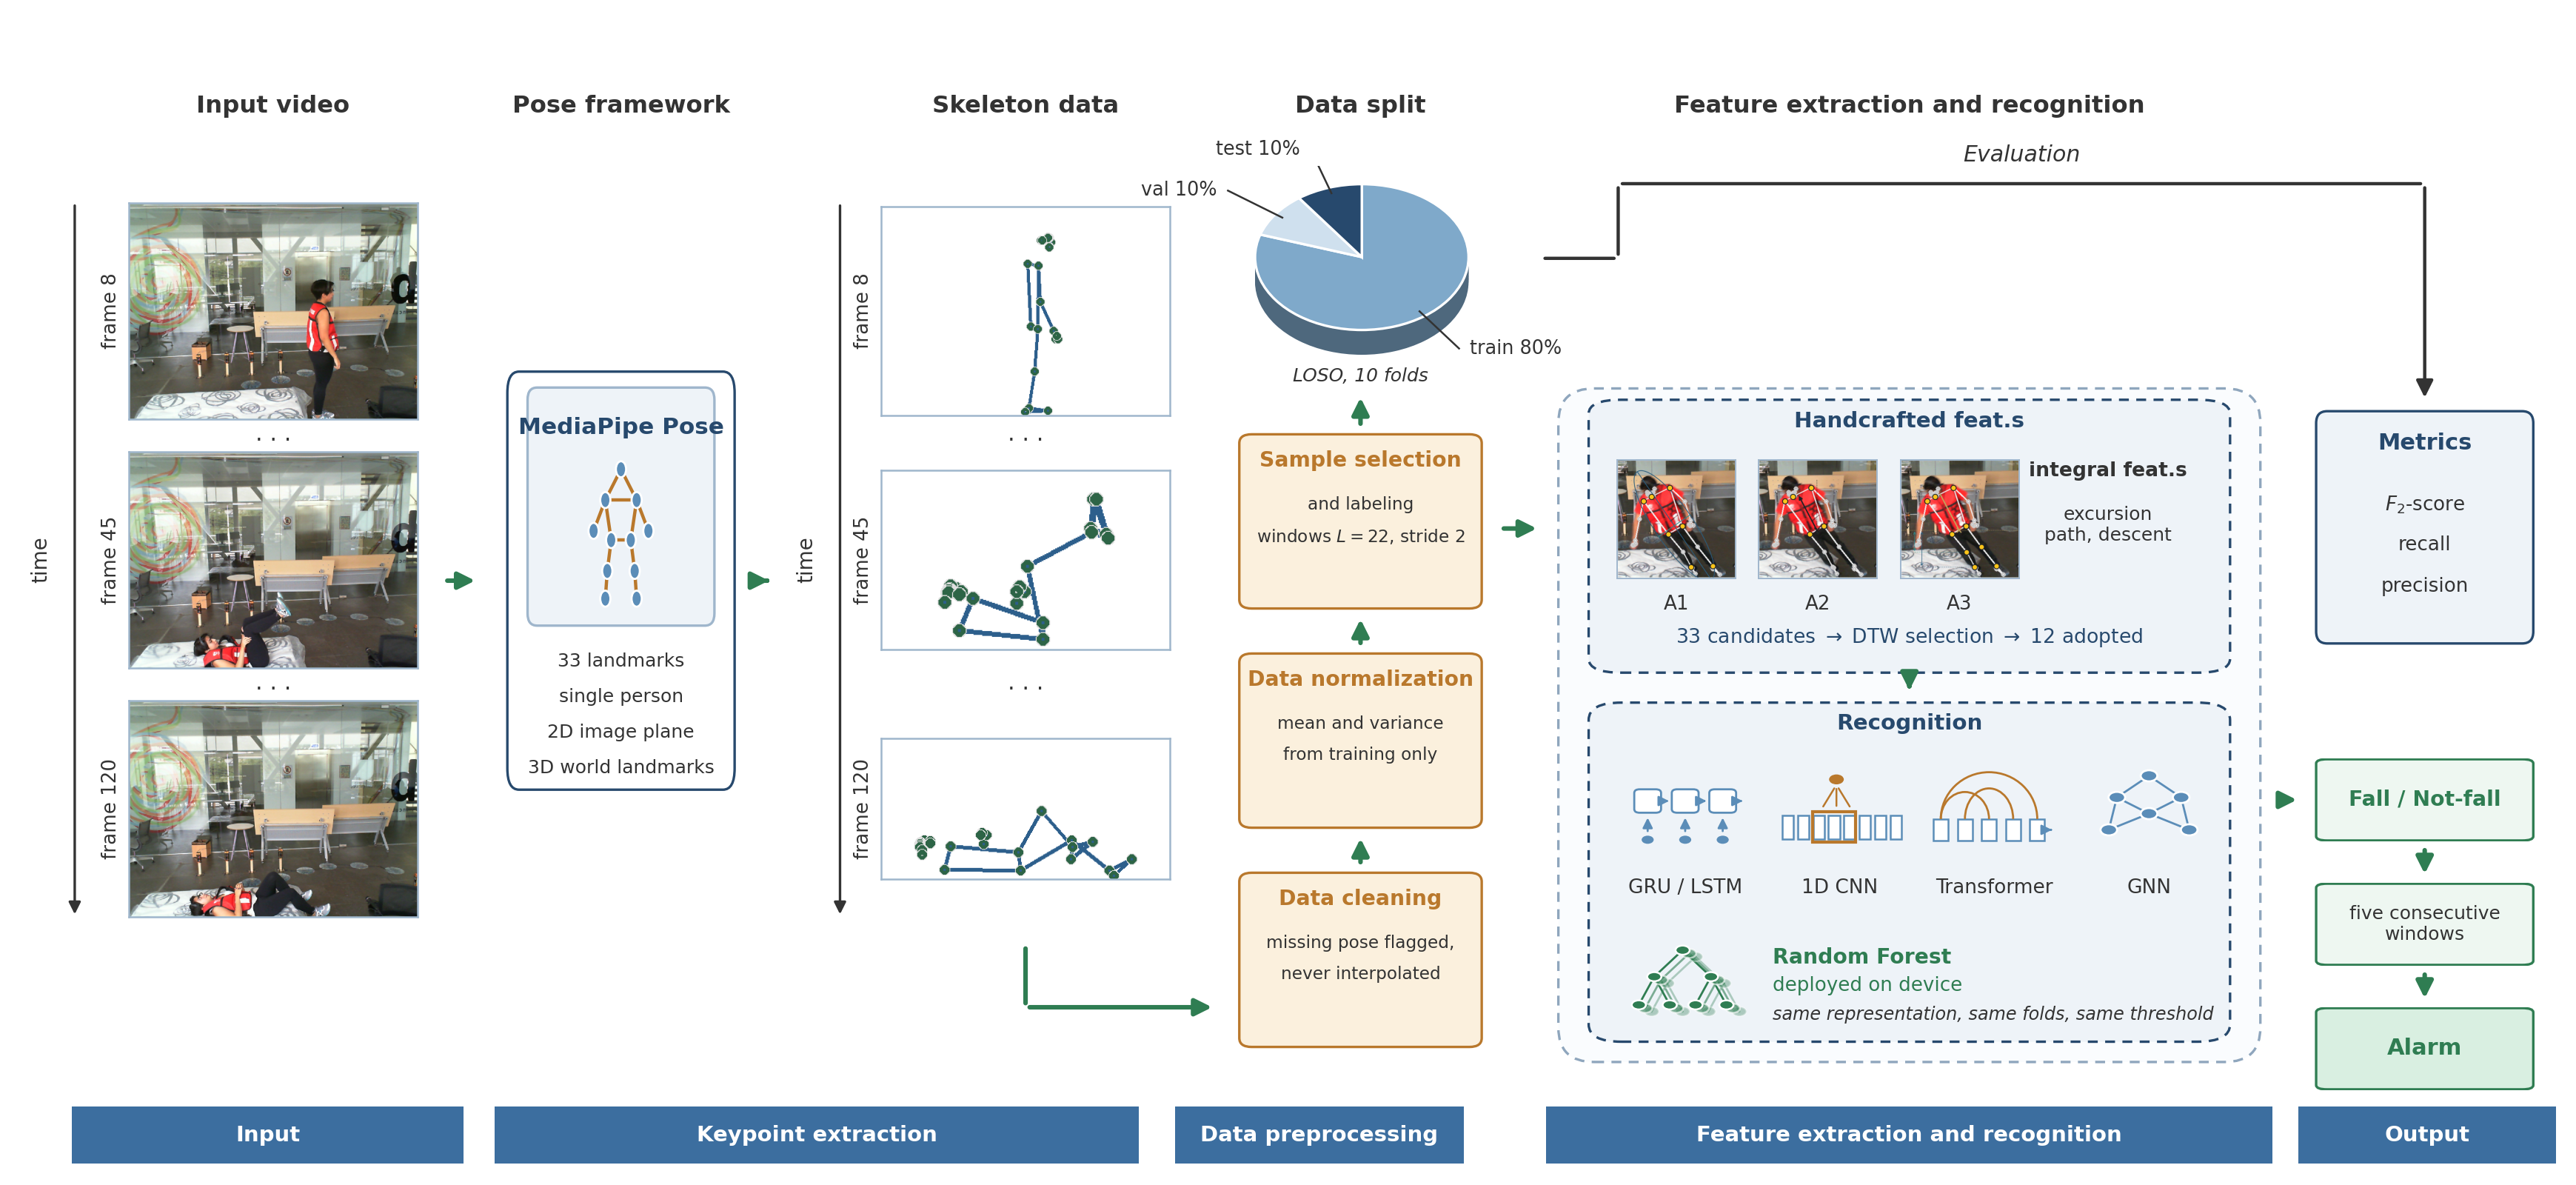
\includegraphics[width=\textwidth]{figure/fig_pipeline_en.png}
\caption{General scheme of the pipeline, from the RGB frame to the generation of the alarm event.}
\label{fig:pipeline}
\end{figure}

Every RGB frame is first turned into a skeletal pose. From the landmarks, 23 geometric and kinematic quantities are derived, to which are added nine quantities computed over longer time intervals and one measure of the position of the hips relative to the floor. This yields 33 candidate features. The set is subsequently reduced by a selection procedure based on \emph{Dynamic Time Warping}, which brings it down to 12 features. These are organised into temporal windows of 22 samples and used as the input of the classifiers.

Six architectures are compared in this work: Random Forest, LSTM, GRU, 1D CNN, Transformer and a graph network. The comparison keeps the input representation and the evaluation protocol unchanged as far as possible, so that what is measured is the contribution of the architecture. For each window the classifier produces a score associated with the presence of a fall. The decisions on the individual windows are finally aggregated over time to obtain the alarm events used during continuous operation. Table~\ref{tab:pipeline_1} summarises the main stages and shows how the information is progressively transformed.

\begin{table}[htbp]
\centering
\caption{Main stages of the pipeline, with their input and output.}
\label{tab:pipeline_1}
\resizebox{\textwidth}{!}{
\begin{tabular}{lllc}
\toprule
\textbf{Stage} & \textbf{Input} & \textbf{Output} & \textbf{Section} \\
\midrule
Pose estimation & RGB frame & 33 landmarks & \ref{sec:pose} \\
Geometric representations & landmarks & 23 quantities & \ref{sec:rappresentazioni} \\
Integral quantities & quantities & $+9$ & \ref{sec:integrali} \\
Height above the floor & quantities & $+1$ & \ref{sec:pavimento} \\
DTW selection & 33 candidates & 12 features & \ref{sec:dtw} \\
Temporal windows & feature sequence & $L=22$, stride 2 & \ref{sec:finestre} \\
Task and labels & windows & three training formulations & \ref{sec:compito} \\
Classifier & $22\times12$ window & score in $[0,1]$ & \ref{sec:classificatori} \\
Aggregation & scores & windows above threshold & \ref{sec:allarme} \\
Alarm event & windows above threshold & a single alert & \ref{sec:allarme} \\
\bottomrule
\end{tabular}
}
\end{table}

The protocol by which the models are evaluated --- LOSO partitioning, normalisation, metrics and decision threshold --- is described instead in Chapter~\ref{cap:sperimentale}.
\section{Experimental data and preprocessing}
\label{sec:dati}

The dataset used to develop the system is UP-Fall. Ten of the seventeen available subjects were considered, together with both views provided by the archive: one lateral, placed approximately at chest height, and one raised frontal. For the ten subjects, all \textbf{220 recordings} available were used, 110 for each camera. Of these, 100 contain falls and 120 ordinary activities of daily living (ADL), for a total of 116.362 frames. No recording was excluded.

UP-Fall does not distribute video files, but sequences of PNG images organised into folders, one per recording. The name of each file carries the timestamp of the instant of acquisition. For every sample, the information concerning subject, camera, recording and label is retained as well. Table~\ref{tab:dati} summarises the data used in the experiments and the main choices adopted for preprocessing.

\begin{table}[htbp]
\centering
\caption{Data used and main preprocessing operations.}
\label{tab:dati}
\begin{tabularx}{\textwidth}{@{}lX@{}}
\toprule
\textbf{Item} & \textbf{Configuration adopted} \\
\midrule
Dataset & UP-Fall \\
Subjects & 10 of the 17 available \\
Views & both cameras \\
Recordings & 220: 100 falls and 120 ADL \\
Frames & 116.362 \\
Recordings excluded & none \\
Declared frame rate & 18 fps \\
Measured frame rate & median 18,09 fps; 14,43--19,63 fps \\
Interpolation & none \\
Subsampling & one frame in two within the windows \\
Missing pose & the temporal sequence is broken \\
Normalisation & estimated within each fold \\
Feature selection & DTW applied once over the whole dataset \\
\bottomrule
\end{tabularx}
\end{table}

\subsection{Temporal cadence}
\label{sec:cadenza}

UP-Fall is declared at 18~fps \cite{MV}, but the timestamps carried by the file names allow the actual cadence to be measured directly. The median frequency is $18{,}09$~fps and ranges between $14{,}43$ and $19{,}63$~fps. In 70 of the 220 recordings the departure from the nominal value exceeds 5\%. The ten recordings furthest from that value all belong to the same individual.

The frequency is not constant within a single recording either. The interval between two consecutive frames has a median of $49{,}6$~ms, a ninth decile of $70{,}2$~ms and a ninety-ninth percentile of $159{,}8$~ms. For the quantities that depend on time, the actual interval $\Delta t_i=t_i-t_{i-1}$ is therefore used, instead of assuming a constant duration of $1/18$~s. This choice matters in the LOSO protocol as well: were the cadence taken as constant, the error on the kinematic quantities would differ from subject to subject and could therefore affect an entire fold.

The coordinates are not resampled onto a uniform time grid, so that no pose is ever created at an instant that was not directly observed. A subsampling is nevertheless applied when the windows are built, taking one frame in two, so that the nominal frequency supplied to the classifier drops from 18 to about 9 samples per second. Resampling to a common length is instead used during the DTW selection described in Section~\ref{sec:dtw}, where the curves are brought to 200 samples before being compared. That operation concerns the analysis of the features and does not alter the data supplied to the classifier.

\subsection{Frame-level labels}

The label of every frame is derived from the suffix \texttt{-0}, \texttt{-1} or \texttt{-2} carried by the name of the PNG file. The three labels denote, respectively, ordinary activity or the phase preceding the fall, the fall transition, and the post-fall state. Where the suffix is absent, the category of the folder is used instead. That decision is not harmless: inside a folder of falls, a frame without a suffix would be labelled as a fall even though the person is still standing. For this reason the program counts the cases in which it had to fall back on the default value and reports them. The resulting distribution is given in Table~\ref{tab:etichette}.

\begin{table}[ht]
\centering
\caption{Distribution of the frame-level labels over the 220 recordings used.}
\resizebox{\textwidth}{!}{
\begin{tabular}{llrr}
\toprule
\textbf{Label} & \textbf{Phase} & \textbf{Frames} & \textbf{Share} \\
\midrule
$0$ & ordinary activity, or the phase preceding the fall & 100.296 & 86,2\% \\
$1$ & fall transition & 5.542 & 4,8\% \\
$2$ & post-fall state & 10.524 & 9,0\% \\
\midrule
\multicolumn{2}{l}{\emph{total}} & 116.362 & 100\% \\
\multicolumn{2}{l}{\emph{with a valid pose}} & 111.570 & 95,9\% \\
\bottomrule
\end{tabular}
}
\label{tab:etichette}
\end{table}

The transition accounts for less than 5\% of the frames available, whereas the post-fall state is almost twice as frequent. This distribution is therefore strongly imbalanced, and it is taken up again both in the definition of the task and in the choice of the evaluation metrics.

Two kinds of interruption are distinguished. When the time interval between two consecutive images is longer than expected, no intermediate frames are reconstructed and the time that actually elapsed is retained. When, by contrast, the estimator returns no valid pose, the sequence is broken and the state used by the temporal features is reset. A window can therefore never span a loss of pose.

A valid pose is available in 95,9\% of the frames. That figure only indicates that the estimator returned a skeletal configuration; it does not measure the quality of the landmarks, which is examined in Section~\ref{sec:posa-mancante}.

The normalisation used by the classifiers is estimated within each fold, on the training data alone. Feature selection by DTW was instead carried out once over the whole dataset, before the LOSO validation, so that the test subject contributes indirectly to the choice of the features. This form of \emph{data leakage} is declared here and measured quantitatively in Section~\ref{sec:misura_leakage} of Chapter~\ref{cap:sperimentale}.

\section{Pose estimation}
\label{sec:pose}

RGB images are the initial data of the pipeline, but they are not used directly by the classifier. Each frame is first turned into a representation of the person's pose by means of a limited set of anatomical points, the \emph{landmarks}.
This transformation reduces the information available to what is essential in order to describe the configuration and the movement of the body. The system thus passes from a dense representation, made of pixels, to a sparse one composed of a few dozen coordinates.
There are two main advantages:
\begin{itemize}
    \item \textbf{reduction of dimensionality}: the system does not have to process hundreds of thousands of pixels directly, but only a limited number of coordinates;
    \item \textbf{interpretability}: each landmark represents a precise part of the body, which allows us to build quantities whose meaning is tied to the geometry and the movement of the person.
\end{itemize}

\subsection{Comparison between estimators}

Three pose estimators were considered over the course of the development; their differences are reported in Table \ref{tab:pose}.

\begin{table}[htbp]
\caption{Main characteristics of the pose estimators considered.}
\label{tab:pose}
\begin{center}
\begin{tabular}{lccc}
\toprule
& \textbf{Points} & \textbf{Coordinates} & \textbf{People} \\
\midrule
MediaPipe \texttt{solutions} & 33 & 2D + world 3D & 1 \\
MediaPipe \texttt{tasks} & 33 & 2D + world 3D & $\geq 1$ \\
YOLOv8-pose & 17 (COCO) & 2D & several people \\
\bottomrule
\end{tabular}
\end{center}
\end{table}

For the construction of the feature dataset, MediaPipe Pose was used in its \texttt{solutions} version, described in Chapter~\ref{cap:stato_arte}. The choice is compatible with UP-Fall, because every recording contains a single subject. The limitation to tracking one person alone is therefore not a problem when the dataset is built. It is a limitation that shows itself rather during operation in a domestic environment.

MediaPipe \texttt{tasks} and YOLOv8-pose were considered as alternatives for execution on the device. YOLOv8-pose uses the \emph{COCO} scheme with 17 two-dimensional landmarks. It can detect several people and can be run on the neural accelerator of the board, but it does not directly provide the same three-dimensional information as MediaPipe. The comparison between the estimators is taken up again in Chapter \ref{cap:edge}, where the computational cost and the behaviour in the presence of several people are also analysed. The $x$ and $y$ coordinates supplied by MediaPipe are normalised with respect to the dimensions of the image and are brought back to pixels through
\[
u=xW,
\qquad
v=yH,
\]

where $W$ and $H$ are the width and the height of the frame. The normalised values are not, however, necessarily contained within $[0,1]$. Over 2.524 frames analysed, the horizontal coordinate leaves the interval in 2,1\% of cases and the vertical one in 12,7\%, reaching a maximum of 1,46. This behaviour is described in Section~\ref{sec:pavimento}. The \emph{world landmarks} are instead used in representation A2. As described in Chapter~\ref{cap:stato_arte}, they are expressed in a three-dimensional reference system centred on the hips \cite{MP}. This information is taken into account in the definition of the A2 features introduced further on.

\subsection{Handling the temporal continuity of the estimator}
\label{sec:tracciatore}

MediaPipe Pose can treat every image independently, or else exploit the temporal continuity between consecutive frames. The second mode is adopted in this thesis, motivated by the fact that the data are sequences belonging to the same recording. The estimator therefore maintains an internal state and uses the information obtained in the previous frame to continue tracking in the frames that follow~\cite{BL}.

This principle is common in \emph{human pose tracking} methods. As discussed in~\cite{SA}, denoting by $\mathbf{x}_i^t$ the position of the $i$-th body part in frame $t$, the tracking process can be represented as

\begin{equation}
\mathbf{x}_{1}^{t*},\ldots,\mathbf{x}_{n}^{t*}
=
\operatorname*{arg\,min}_{\mathbf{x}_{1}^{t},\ldots,\mathbf{x}_{n}^{t}}
f\left(
\mathbf{x}_{1}^{t},\ldots,\mathbf{x}_{n}^{t}
\mid
\mathbf{x}_{1}^{t-1},\ldots,\mathbf{x}_{n}^{t-1}
\right).
\label{eq:pose_tracking}
\end{equation}

where $n$ is the number of body parts considered and $\mathbf{x}_{i}^{t*}$ represents the estimated position of part $i$ in the current frame. The function $f$ takes into account not only the information present in the frame at time $t$, but also the configuration observed in the previous frame. It is precisely this temporal dependence that distinguishes tracking from pose estimation carried out on independent images. The same notion of temporal continuity is present in the use of MediaPipe Pose in video mode. Once the person has been located, the information derived from the landmarks of the previous frame is used to continue tracking in the frames that follow \cite{BL}.

\begin{figure}[htbp]
    \centering
    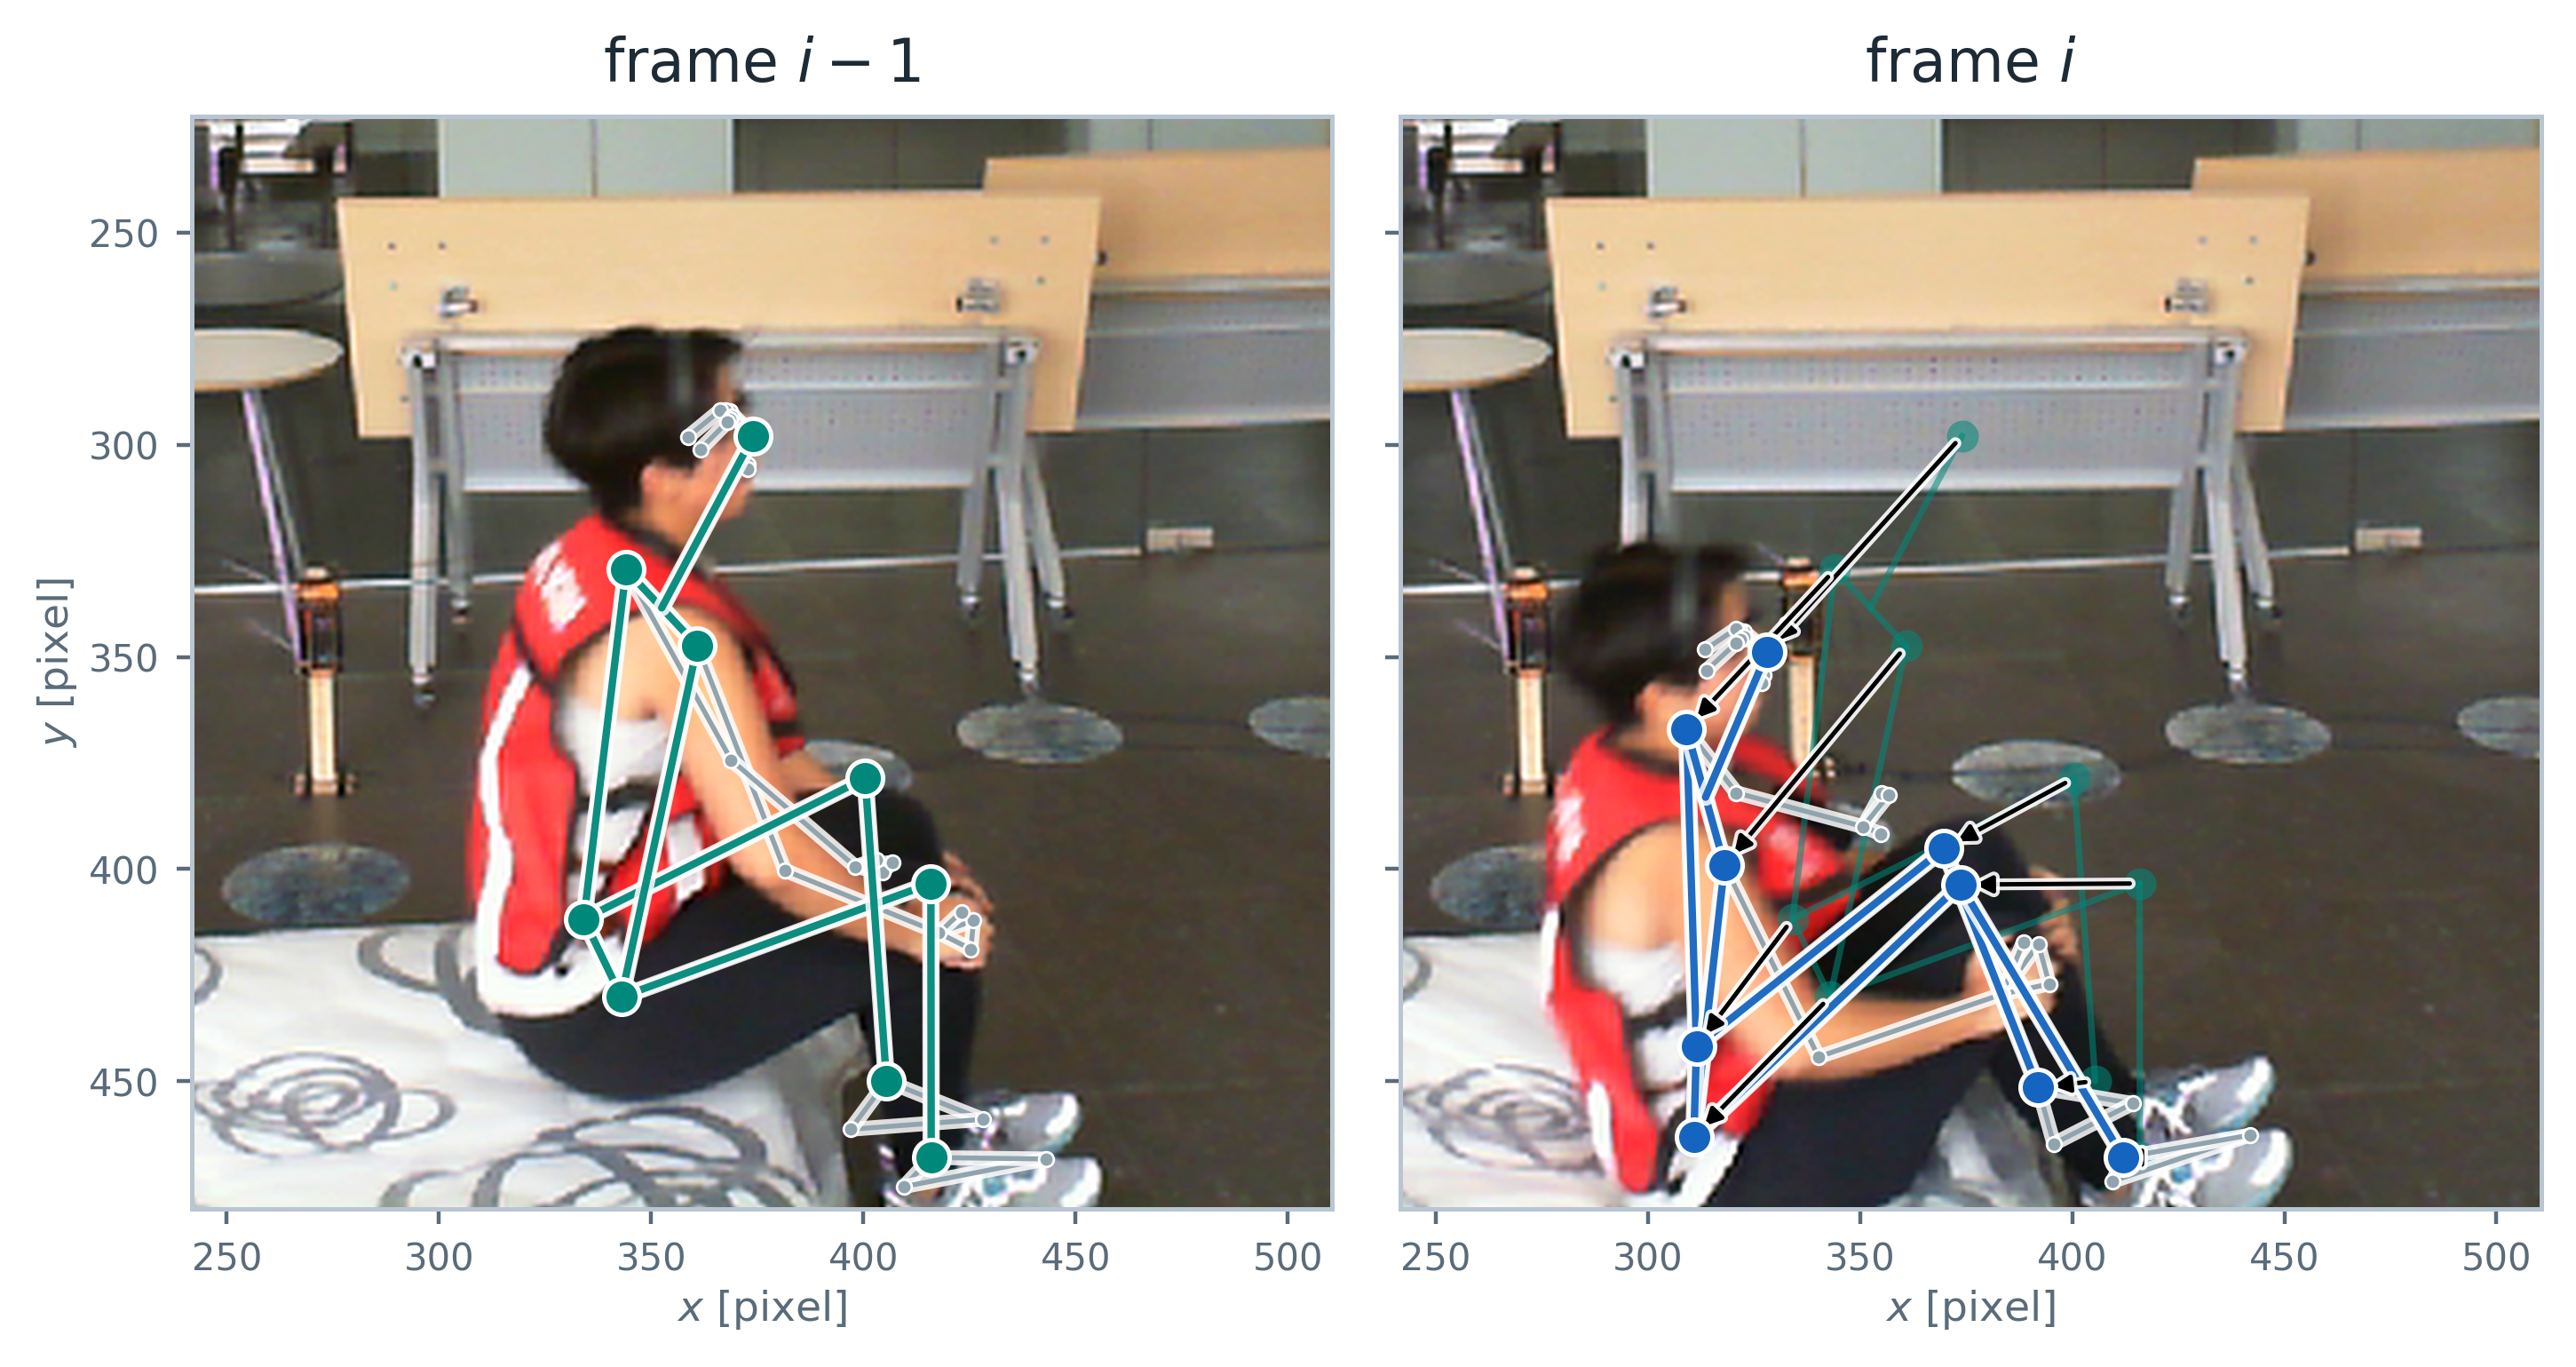
\includegraphics[width=\linewidth]{figure/fig_tracciatore_en.png}
    \caption{Two consecutive frames of a fall (\texttt{sub09\_act05\_trial01}, camera 1, frames 28 and 29). On the left the pose at frame $i-1$; on the right the pose at frame $i$, with the previous one superimposed in transparency}
\label{fig:tracciatore}
\end{figure}

This continuity must, however, be broken when a recording ends. Denoting by $r$ a recording, no previous pose belonging to video $r-1$ must be available at the beginning of the sequence. Using the same notation as Equation~\ref{eq:pose_tracking}, this condition can be expressed as
\begin{equation}
\mathbf{x}^{0,(r)} = \varnothing
\qquad \text{for every } r ,
\label{eq:azzeramento}
\end{equation}

where $\mathbf{x}^{0,(r)}$ denotes the absence of a previous pose at the beginning of recording $r$. Every recording thus starts from an empty state, which is obtained by creating a new estimator at the beginning of each one and closing it at the end. The temporal state is in this way maintained between frames that genuinely belong to the same sequence.
Creating the estimator introduces a few tenths of a second of initialisation, while closing it frees the resources used and prevents the TensorFlow Lite instances from accumulating while the whole archive is processed.

During offline extraction all frames are processed in order, and the program waits for the pose estimation and the computation of the features to be completed before moving on to the next frame.
On the edge device, by contrast, frames arrive continuously from the camera, and the time required for pose estimation determines how many of them can actually be processed.
The processing chain therefore remains the same, but the time constraint changes. This difference is analysed in Chapter~\ref{cap:edge}.

\subsection{Absence of the pose and instability of the coordinates}
\label{sec:posa-mancante}

The landmarks returned by the estimator are not exact measurements of the position of the body, but estimates derived from the image. Their quality can therefore be affected by various factors, such as occlusions, viewpoint or the configuration assumed by the person. Three events may occur:
\begin{enumerate}
    \item the landmark is estimated, but the estimator considers it poorly visible;
    \item the estimator fails to reconstruct a valid pose;
    \item the pose is found, but the coordinates oscillate slightly from one frame to the next.
\end{enumerate}

As regards the first case, MediaPipe returns for each landmark a \emph{visibility} value, associated with the probability that the point is visible in the image \cite{BL}. This value is not used directly in the pipeline: when the pose is available, the geometric engine uses the coordinates of the points needed to build the features.

Visibility was nonetheless analysed over 26.548 frames with a valid pose. Nose, shoulders and hips show median values above $0{,}98$. The situation differs for some points of the limbs: the median visibility of the elbows, for instance, drops from $0{,}81$ to $0{,}52$ when the person is on the ground. The difference is even more marked in lateral recordings: the knee and the ankle on the side further from the camera show values below $0{,}5$ in more than half of the frames, whereas on the side facing the camera they remain around $0{,}9$.

Using visibility as the sole criterion for accepting or rejecting the entire pose did not produce a useful selection. With a threshold of $0{,}5$, all the frames analysed continue to be considered valid, because the main points of the trunk retain very high values. A use of visibility at the level of the individual landmark was not explored in this work. The effect of perturbations applied to the different points is, however, taken up again in Section~\ref{sec:occlusioni}.

The second case concerns the complete absence of the pose. In $4{,}1\%$ of the frames, that is 4.792 cases out of 116.362, the estimator returns no valid pose; the percentage rises to $19\%$ on the external archive examined later. The pipeline identifies these samples through the variable \texttt{ha\_posa}, which equals 1 when the pose is available and 0 when it is absent. In the latter case the features are set to zero, but that value is not treated as a real measurement. Making this distinction is essential, because zero can have a physical meaning: a trunk angle equal to zero, for example, may correspond to a configuration that was actually observed.

When the pose is lost, the temporal state used by the dynamic features is also reset, so as to avoid computing a derivative that compares a sample preceding the loss of tracking with one acquired after tracking has resumed.
The same criterion was applied when building the windows: a window can be constructed only within a continuous stretch, so as not to create sequences that span intervals in which the movement was not actually observed.

The third problem concerns the stability of the coordinates. Even when the pose is available, the landmarks may vary slightly between consecutive frames. Part of this difference is due to the real movement of the person, and part to the uncertainty of the estimate. This phenomenon, known as \emph{jitter}, affects above all the quantities obtained from temporal differences. To quantify it, the displacement of each landmark between two consecutive frames was measured. The displacement of the centre of the hips was subtracted in order to reduce the effect of the overall translation of the person, and the result was normalised with respect to the length of the trunk.

\begin{figure}[htbp]
\centering
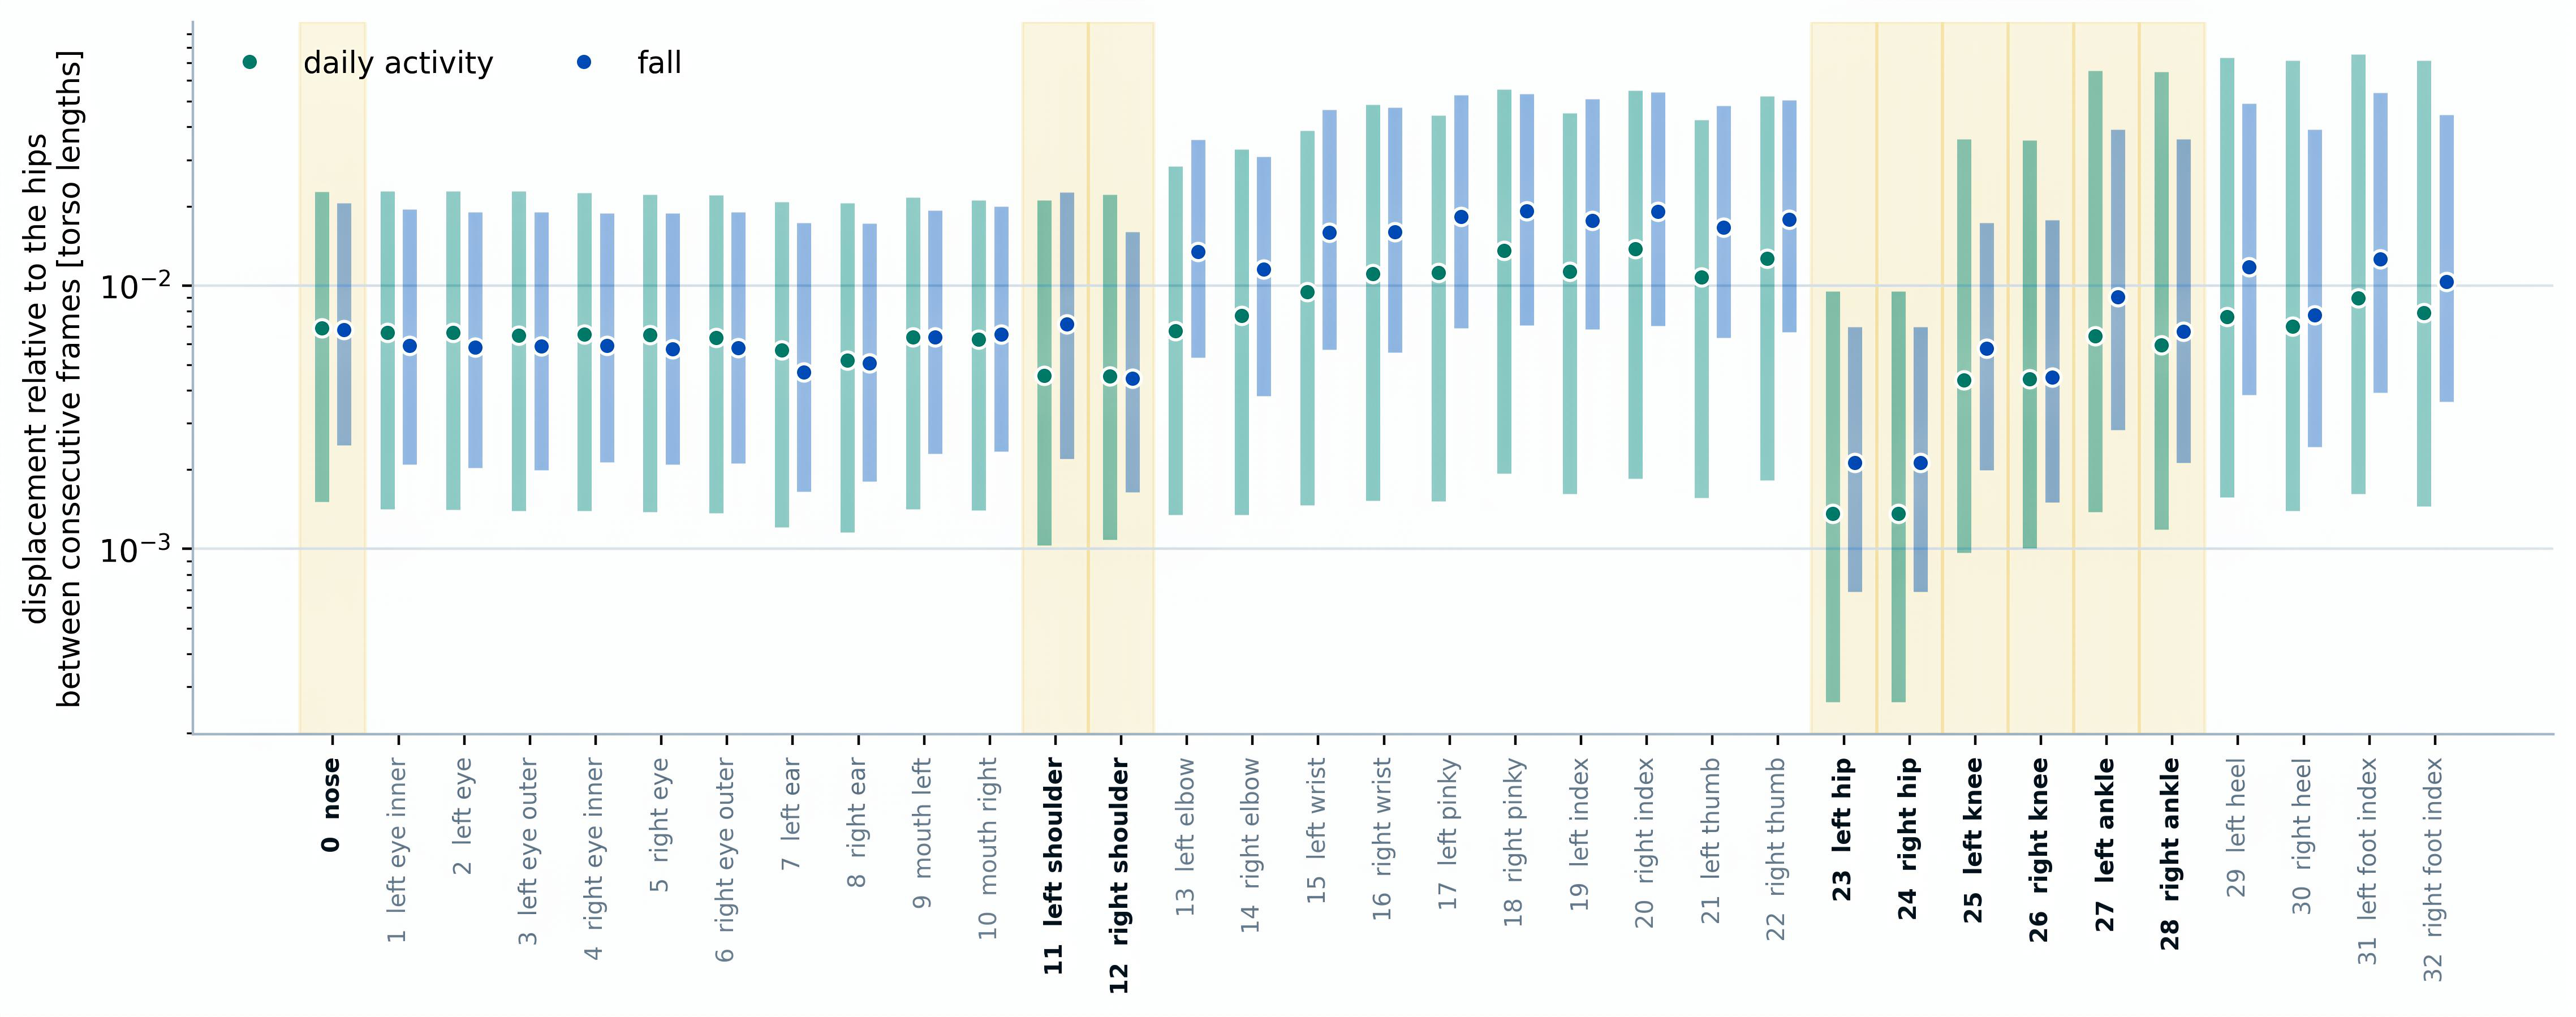
\includegraphics[width=1\textwidth]{figure/fig_spostamento_en.png}
\caption{Displacement of the landmarks between consecutive frames, measured with respect to the centre of the hips and normalised by the length of the trunk.}
\label{fig:spostamento}
\end{figure}

The points of the trunk and of the lower limbs show smaller displacements than the wrists and the fingers. The difference remains visible in the fall recordings as well, where the overall movement increases.
The representations developed rest mainly on the head, the trunk and the lower limbs, and build no features from the landmarks of the hands.

\subsection{Temporal filtering and derivatives}
\label{sec:filtraggio}

One possible remedy for the instability of the landmarks is to apply a temporal filter. During the initial development phase an \emph{Exponential Moving Average} was considered,
\[
\tilde{x}t=
\alpha x_t+
(1-\alpha)\tilde{x}{t-1},
\]

but this option was not subsequently applied to the dataset used in the experiments.
The features are computed directly on the landmarks returned by MediaPipe. In the absence of filtering, the quantities obtained through temporal differences may therefore be more affected by the oscillations. A velocity, for example,
\[
v_i = \frac{x_i-x_{i-1}}{\Delta t_i},
\]
is influenced by the difference between two coordinates, both subject to the uncertainty of the
estimator. Consequently, when the representations were built, only the dynamic quantities considered useful were retained, while the second derivatives present in the earliest versions were removed.

The derivatives retained are computed on the basis of the time that actually elapsed between two consecutive frames. Denoting by $t_i$ the time of the current frame,
\[
\Delta t_i = t_i-t_{i-1}.
\]

In the earliest versions of the pipeline the interval was instead derived from the nominal acquisition frequency. Since, as shown in Section~\ref{sec:cadenza}, the actual cadence is constant neither between recordings nor within a single recording, the final configuration uses the timestamps of the frames directly. In order to describe the movement over a wider time interval as well, some integral quantities were moreover introduced, defined in Section~\ref{sec:integrali}.

\section{Geometric representations of movement}
\label{sec:rappresentazioni}

Once the pose has been estimated, the coordinates of the landmarks must be turned into quantities that describe the configuration and the movement of the person. Three representations of the same movement were built. They do not correspond to different classifiers, but to three different ways of turning the pose into numerical features:
\begin{itemize}
    \item \textbf{A1} works in the image plane and describes mainly the shape and the orientation of the distribution of the landmarks.
    \item \textbf{A2} uses the \emph{world landmarks} supplied by MediaPipe and builds a three-dimensional representation.
    \item \textbf{A3} uses two-dimensional coordinates referred to the geometry of the body, taking the hips as the origin and the length of the trunk as the normalisation factor.
\end{itemize}

The three representations are built before feature selection. The quantities obtained therefore converge into the same set of candidates, and the procedure described in Section~\ref{sec:dtw} establishes which of them to keep in the final representation.
Table~\ref{tab:landmark_rappresentazioni} reports the sets of points needed to build the quantities of the three representations, while Figure \ref{fig:rappresentazioni} shows those sets on a real pose from the dataset, with the index of each point beside the point itself.

\begin{table}[ht]
\centering
\caption{Landmarks used in the three geometric representations.}
\label{tab:landmark_rappresentazioni}
\resizebox{\textwidth}{!}{
\begin{tabular}{llcl}
\toprule
\textbf{Representation} &
\textbf{MediaPipe indices} &
\textbf{No.} &
\textbf{Landmarks used} \\
\midrule
A1 & 0, 11, 12, 23, 24, 27, 28
   & 7 & nose, shoulders, hips, ankles \\
A2 & 0, 11, 12, 23, 24
   & 5 & nose, shoulders, hips \\
A3 & 0, 11, 12, 23--28
   & 9 & nose, shoulders, hips, knees, ankles \\
\bottomrule
\end{tabular}
}
\end{table}

\begin{figure}[htbp]
    \centering
    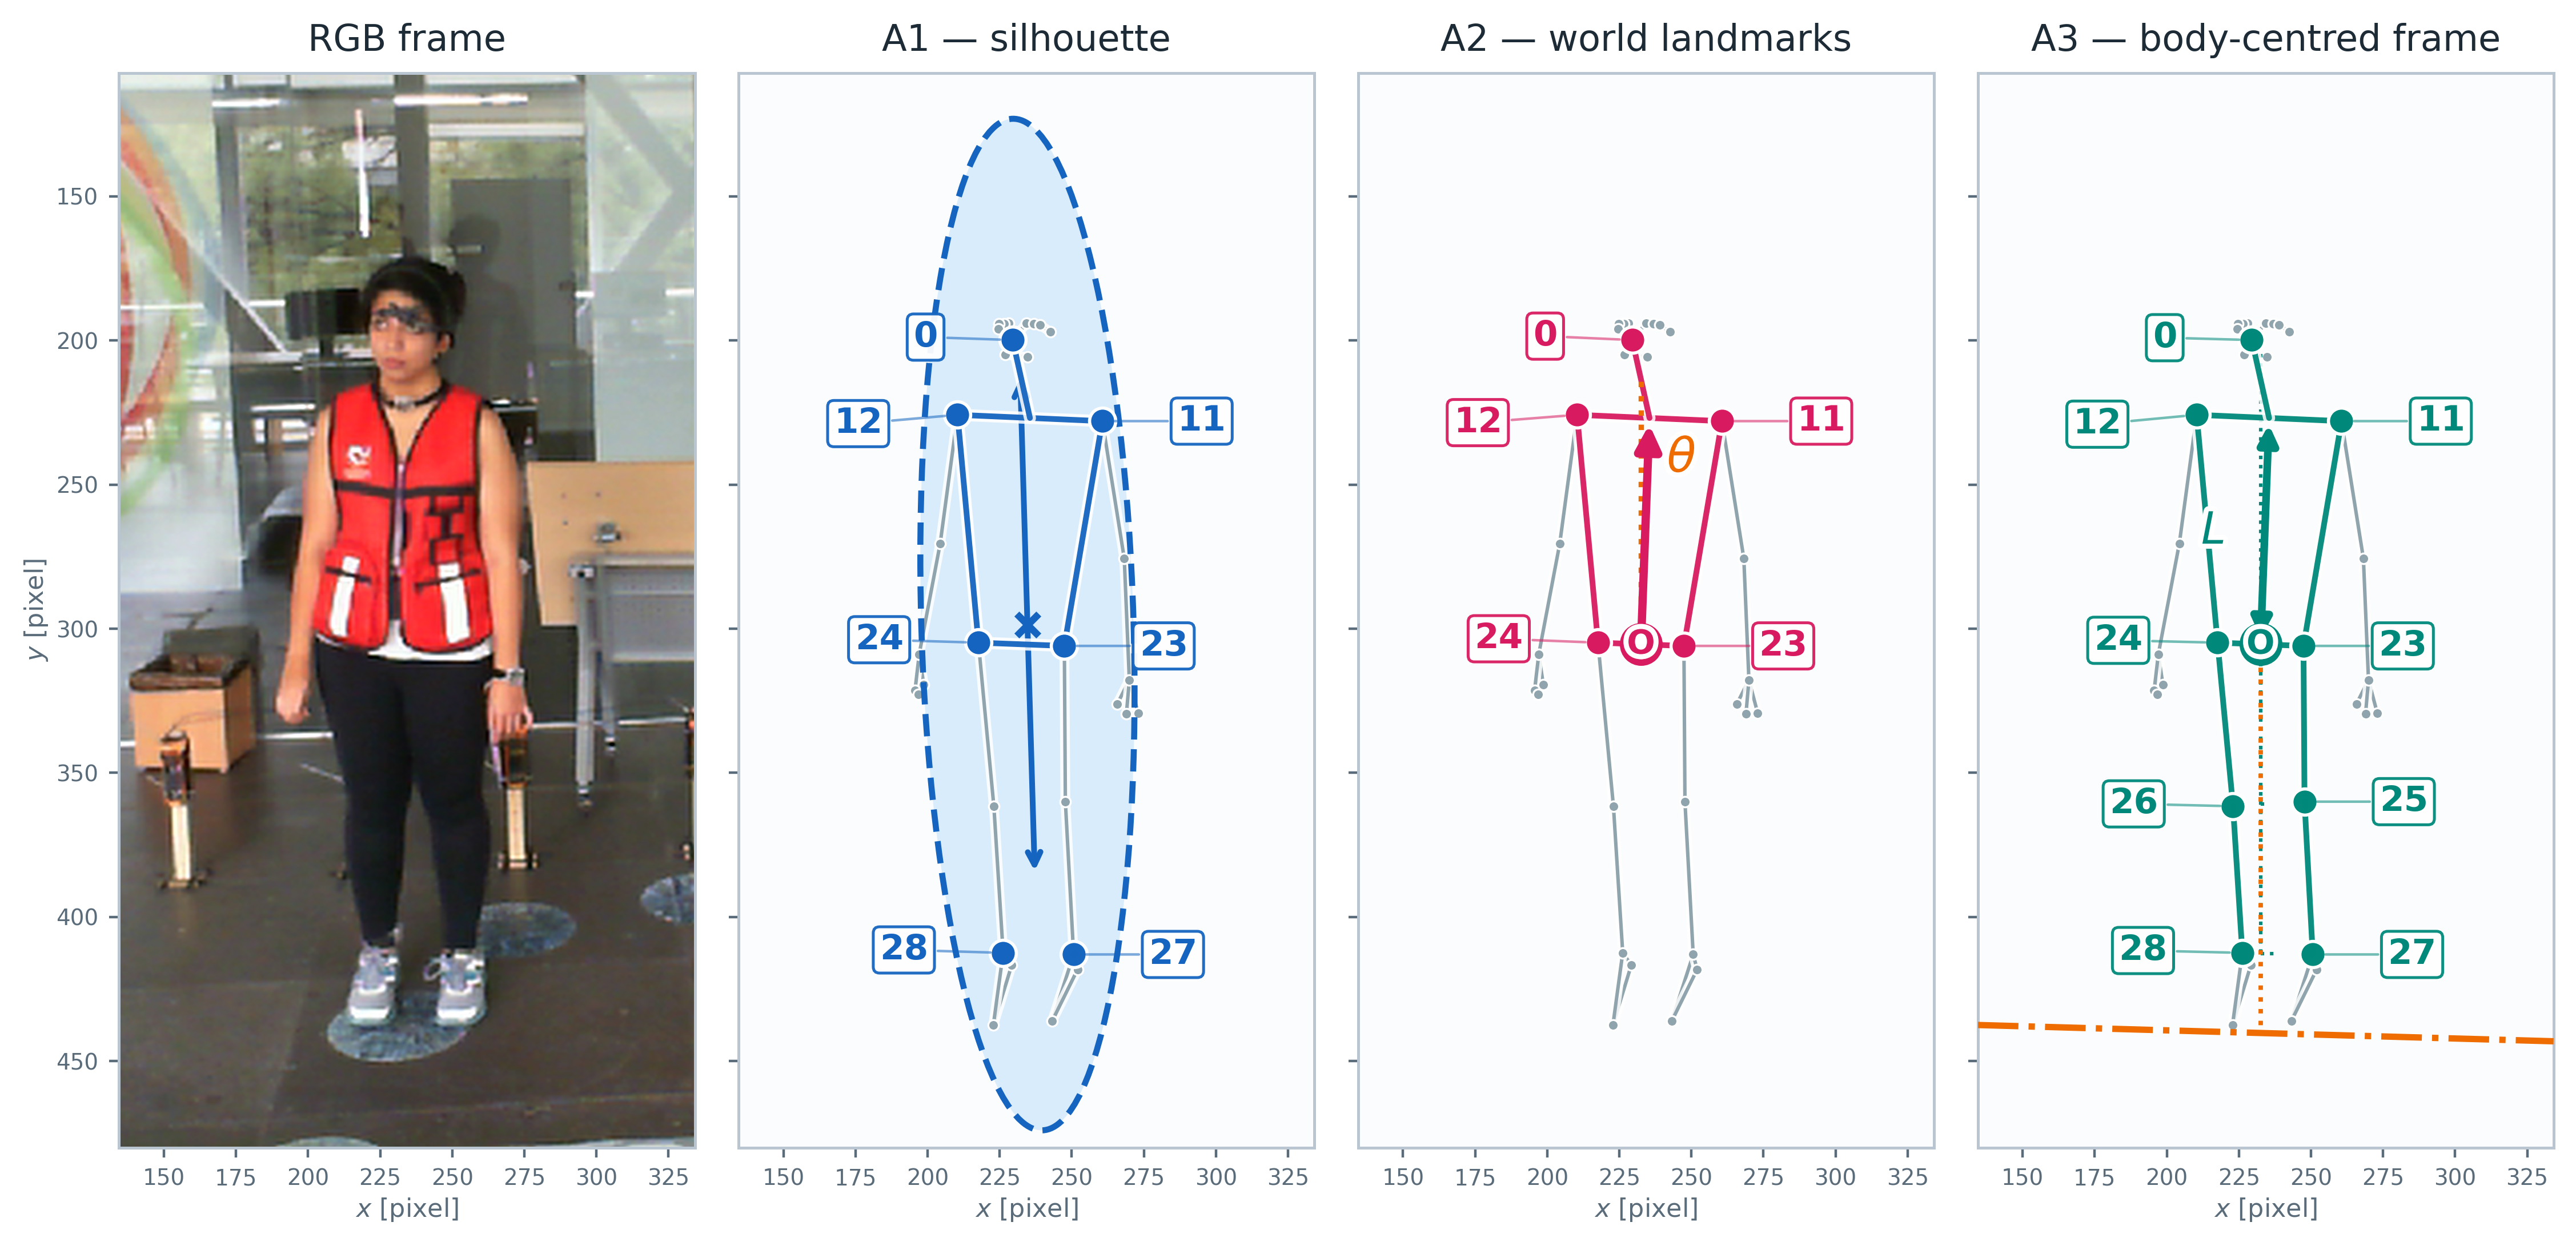
\includegraphics[width=1\linewidth]{figure/fig_landmark_en.png}
    \caption{The set of landmarks of the three representations}
    \label{fig:rappresentazioni}
\end{figure}

\subsection{A1: description of the silhouette in the image plane}

Representation A1 uses the landmarks listed in Table \ref{tab:landmark_rappresentazioni} as a distribution of points in the image plane. The anatomical connections are not used directly, because what matters is the overall shape assumed by the body. From a geometric point of view, this cloud can be described by an ellipse, where the major axis represents the dominant orientation of the body, the minor axis the dispersion in the orthogonal direction, and the ratio between them describes its elongation.

The ellipse is derived from the covariance matrix of the landmarks. Denoting by $J$ the set of points used and by $p_j\in\mathbb{R}^2$ the position in pixels of point $j$, the centre of the distribution is computed:
\begin{equation}
\bar{p} =
\frac{1}{|J|}
\sum_{j\in J} p_j .
\label{eq:centroide_a1}
\end{equation}

The covariance matrix is
\begin{equation}
S =
\frac{1}{|J|-1}
\sum_{j\in J}
\left(p_j-\bar{p}\right)
\left(p_j-\bar{p}\right)^{\top}.
\label{eq:covarianza}
\end{equation}

which makes it possible to identify the two principal directions of the point cloud through its eigenvalues and eigenvectors:
\begin{equation}
S\,v_k = \lambda_k v_k,
\qquad
\lambda_1 \geq \lambda_2 \geq 0,
\qquad
v_1 \perp v_2 .
\label{eq:autovalori}
\end{equation}

The eigenvector $v_1$ describes the direction along which the body is most widely distributed, while the eigenvector $v_2$ identifies the orthogonal direction. The dimensions along the two axes are
\begin{equation}
a = \sqrt{\lambda_1},
\qquad
b = \sqrt{\lambda_2},
\label{eq:assi_a1}
\end{equation}

The ratio
\begin{equation}
\rho = \frac{a}{b}
\label{eq:allungamento_a1}
\end{equation}
measures how elongated or compressed the configuration appears, while the inclination of the principal axis is obtained from
\begin{equation}
\theta =
\operatorname{atan2}\left(v_{1y},v_{1x}\right).
\label{eq:angolo_a1}
\end{equation}

Nine quantities are extracted from A1: \textbf{the two semi-axes $a$ and $b$; the ratio $\rho=a/b$; the inclination $\theta$ of the principal axis, expressed in degrees; the temporal variations of $a$, of $\rho$ and of $\theta$; the horizontal and vertical components of the velocity of the centre $\bar{p}$, normalised with respect to the dimensions of the image.}

The example reported in Figure~\ref{fig:momenti_a1} shows the geometric meaning of the representation at two moments of the same fall. In an upright position the ellipse is oriented mainly vertically; when the person is on the ground, the principal axis instead takes on an almost horizontal direction.
\begin{figure}[htbp]
\centering
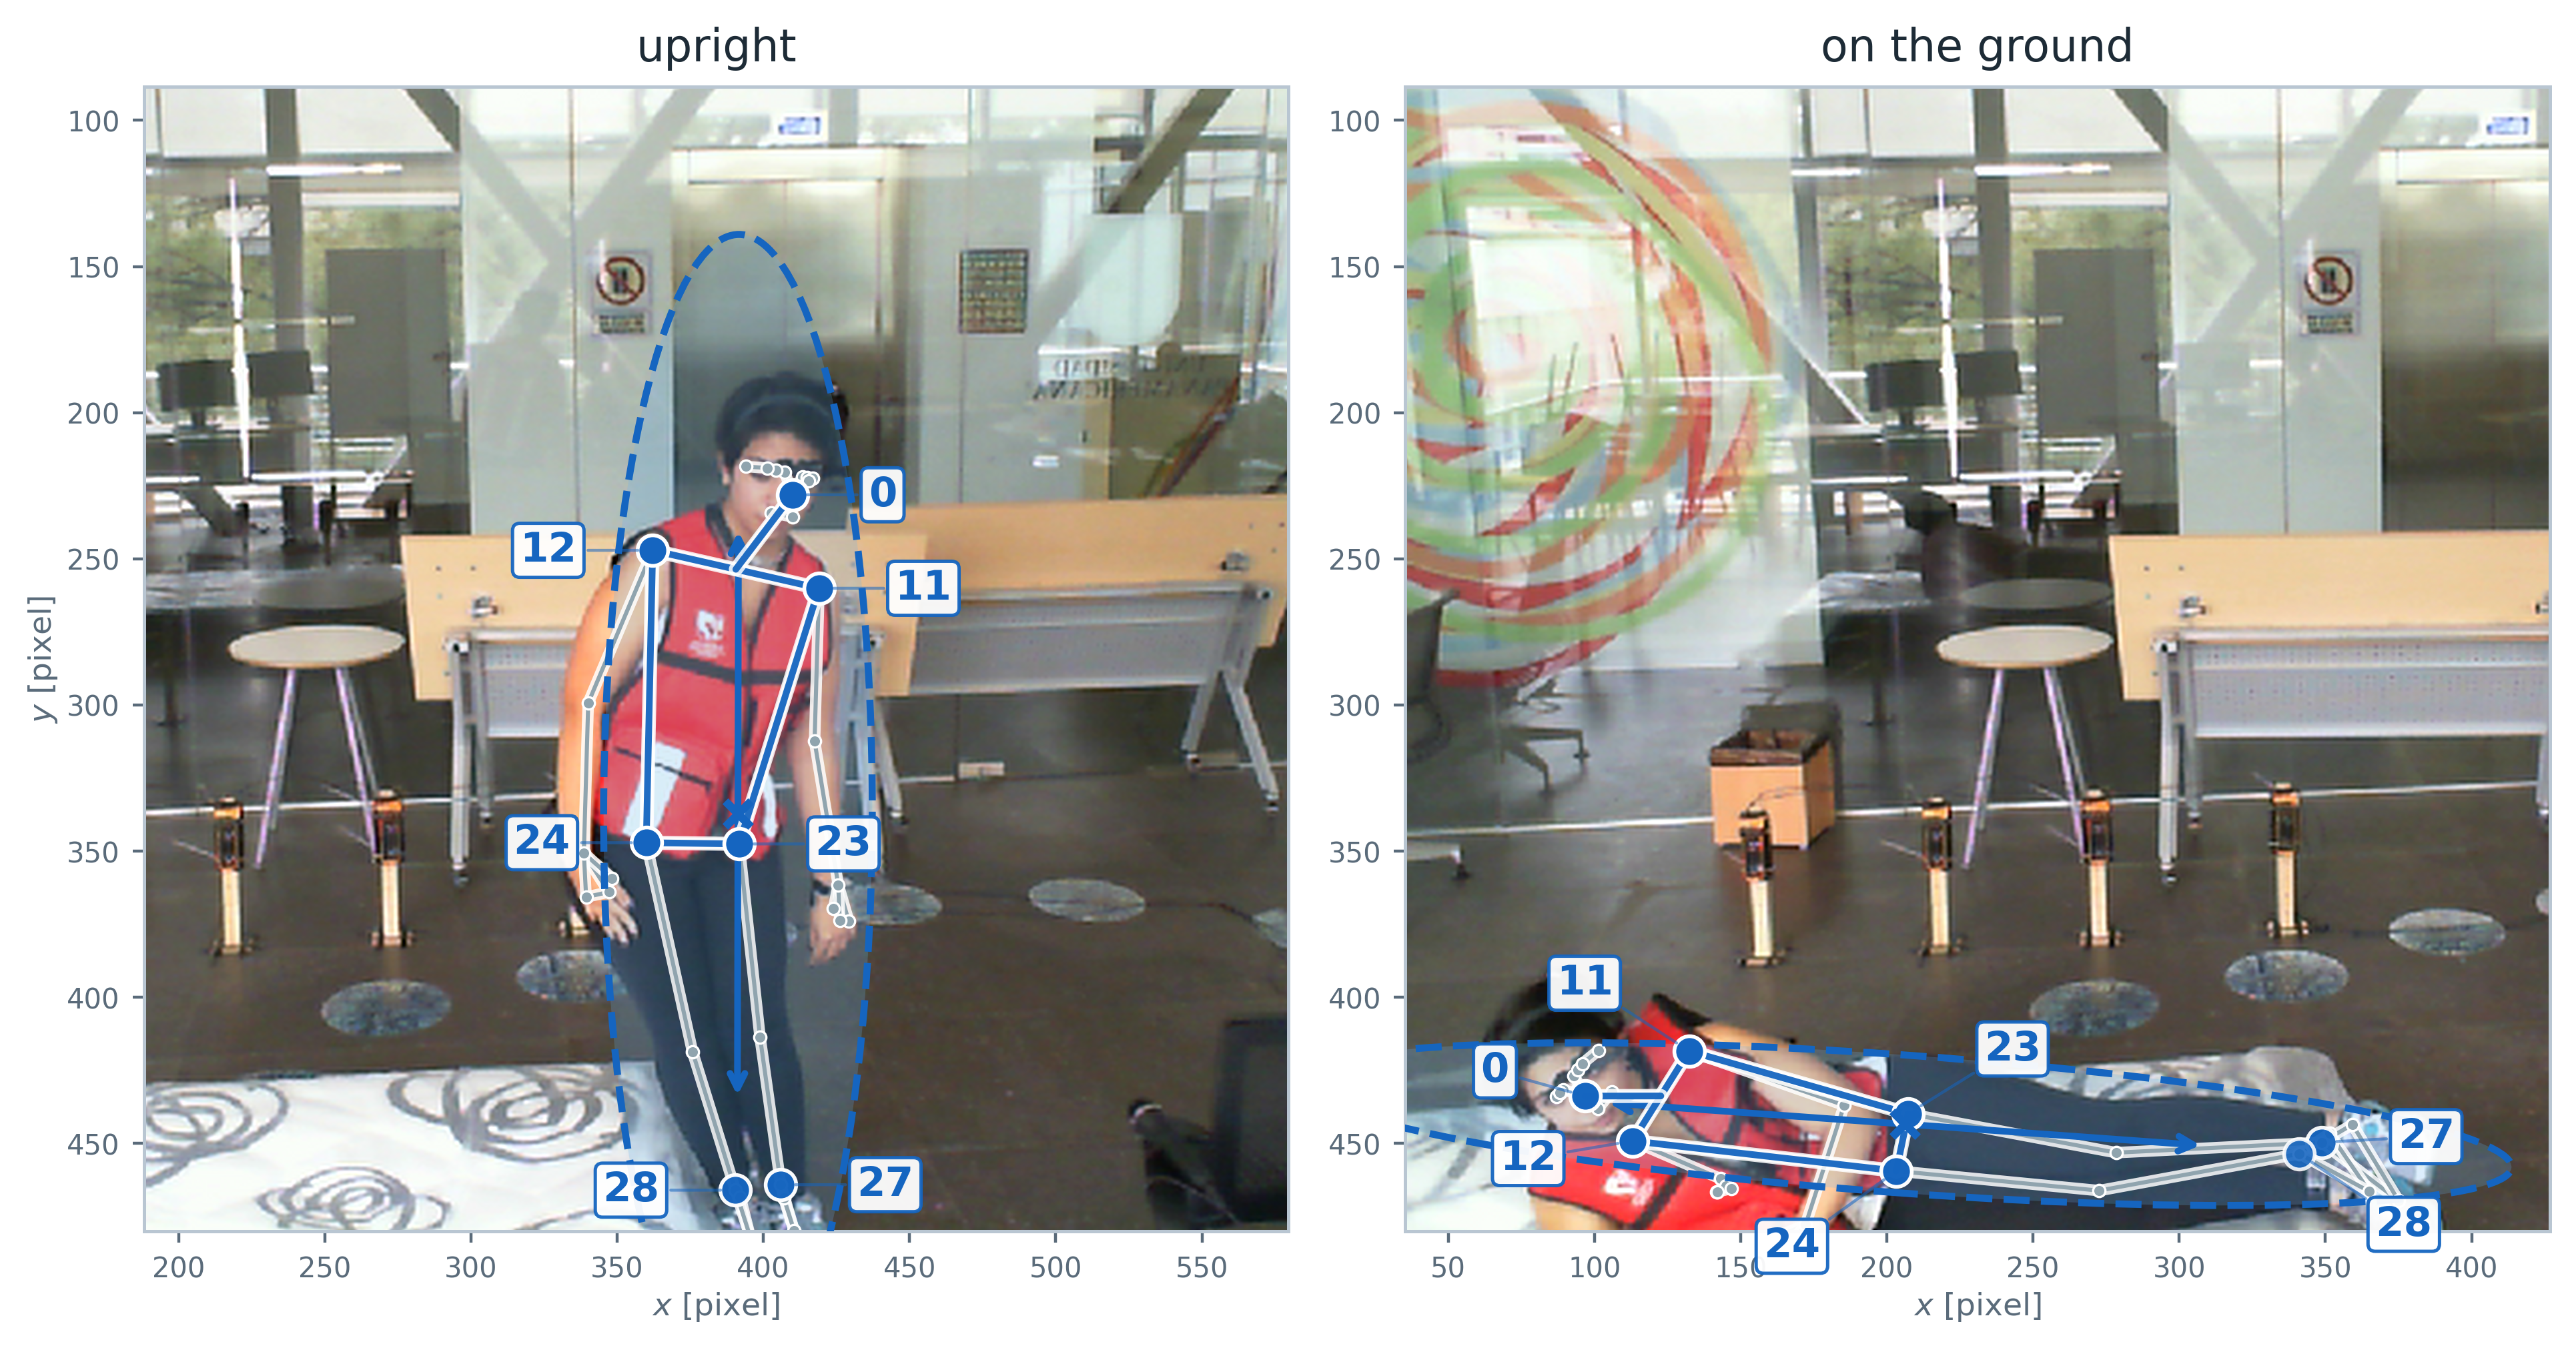
\includegraphics[width=\textwidth]{figure/fig_momenti_a1_en.png}
\caption{Representation A1 at two instants of the same fall
(\texttt{sub09\_act04\_trial01}, camera 1).}
\label{fig:momenti_a1}
\end{figure}

The main limitations of A1 stem from the fact that all the quantities are computed in the plane of the image. The same posture may therefore look different when the viewpoint of the camera changes; and because the principal axis of the ellipse has no direction, an axis oriented at $30^\circ$ is equivalent to the same axis represented at $210^\circ$. The orientation therefore has a periodicity of $180^\circ$. Before its temporal variations are computed, the angle is therefore unwrapped so as to account for that periodicity, avoiding numerical jumps in depth.

\subsection{A2: three-dimensional description}

Representation A2 uses the \emph{world landmarks}, again those listed in Table \ref{tab:landmark_rappresentazioni}. Unlike the coordinates in the image plane, every point is described by three coordinates and therefore also retains information about depth.
The main quantities are built starting from the trunk vector. Denoting by
$p_{s_L}$ and $p_{s_R}$ the two shoulders and by $p_{h_L}$ and $p_{h_R}$ the two hips, the respective midpoints are computed

\begin{equation}
p_s = \frac{p_{s_L}+p_{s_R}}{2},
\qquad
p_h = \frac{p_{h_L}+p_{h_R}}{2}.
\end{equation}

The vector $t = p_s-p_h $ describes the direction of the trunk in three-dimensional space.
The five quantities derived from this representation are:\textbf{trunk angle, variation of the trunk angle, magnitude of the angular velocity of the trunk, velocity of the head and vertical position of the head with respect to the hips.} Figure~\ref{fig:momenti_a2} shows the trunk vector at the same two instants used for A1.

\begin{figure}[htbp]
\centering
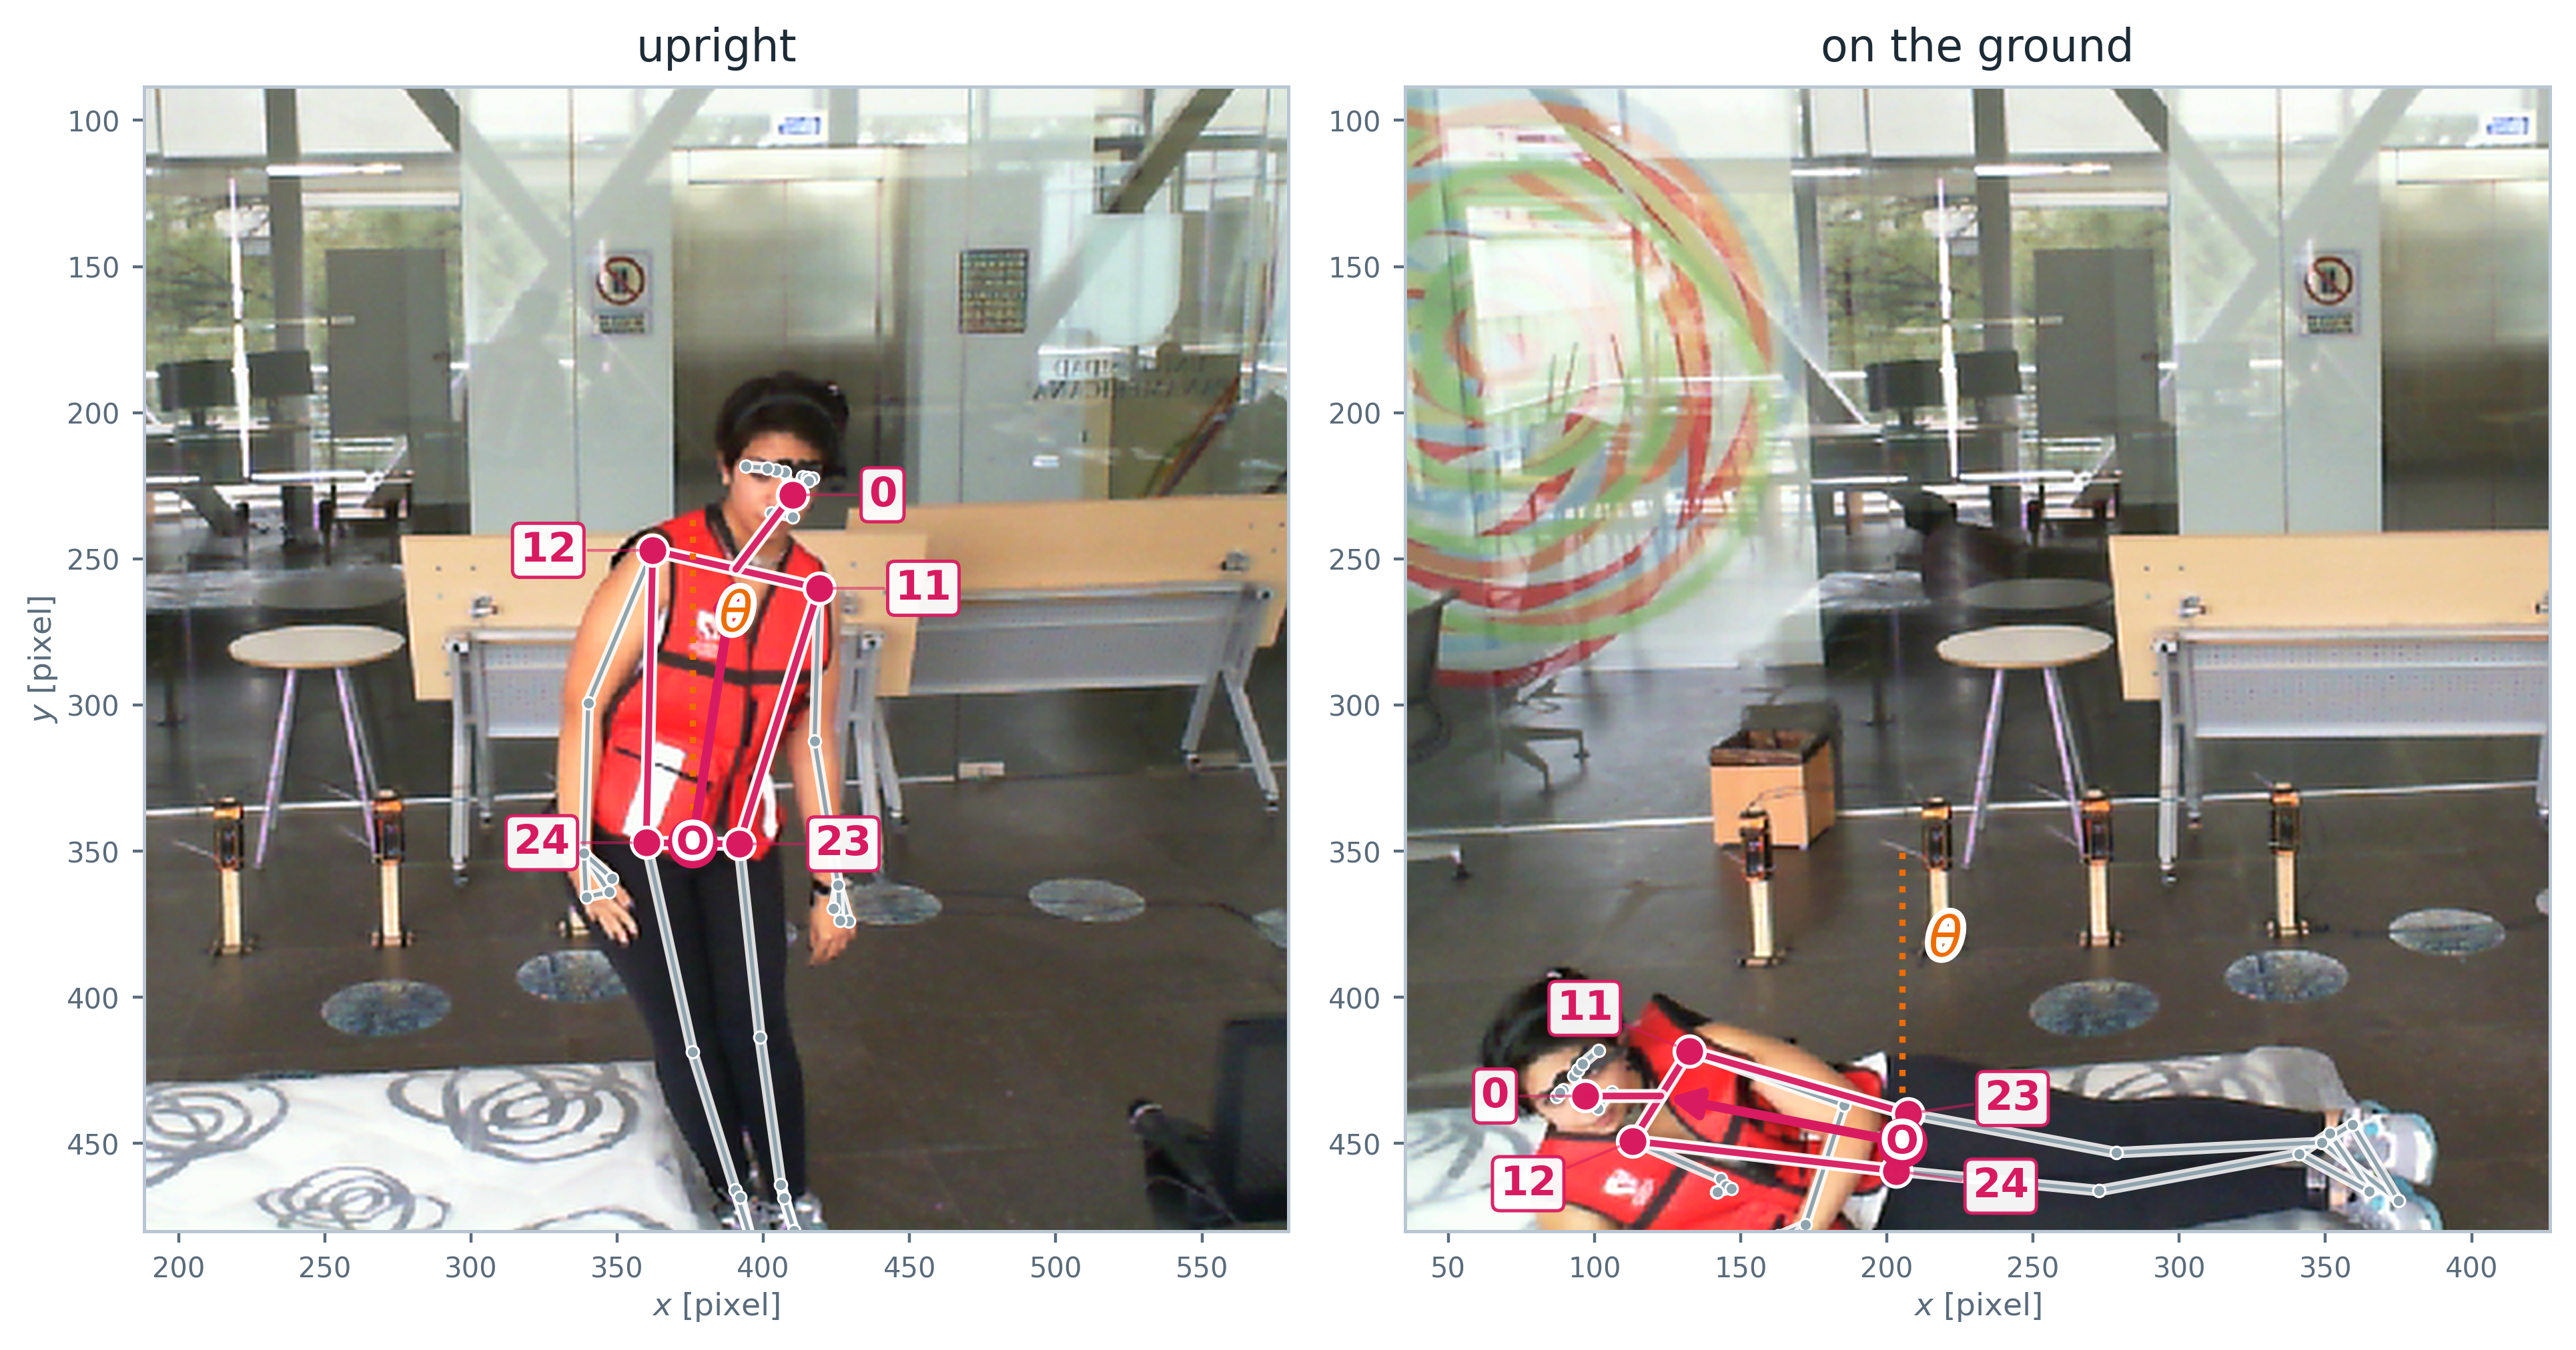
\includegraphics[width=\textwidth]{figure/fig_momenti_a2_en.png}
\caption{Representation A2. The angle goes from $8{,}96^\circ$ in an upright position to $-79{,}13^\circ$ on the ground. The point O marks the centre of the hips, the origin of the reference system of the \emph{world landmarks}.}
\label{fig:momenti_a2}
\end{figure}

The \emph{world landmarks} must, however, be interpreted with respect to their own reference system, which is centred on the hips and does not coincide with an absolute coordinate system of the room. Consequently, the trunk angle does not represent an absolute inclination with respect to the floor or to the direction of gravity. This characteristic is most apparent in the position of the hips which, being the origin of the reference system, remains practically constant by construction. Over forty consecutive frames the standard deviation of its position is $3\cdot10^{-5}$ metres for the hips, against about $1{,}75\cdot10^{-2}$ metres for the nose.

The quantities relating to the translation of the hips, present in the initial formulation, were therefore measuring mainly numerical variations and were removed. For the same reason, in the integral quantities of A2 the nose is followed rather than the centre of the hips.

\subsection{A3: description referred to the geometry of the body}

Representation A3 again uses two-dimensional landmarks, but expresses them with respect to the geometry of the person. The centre of the hips is taken as the origin of the reference frame, while the distance between the centre of the hips and the centre of the shoulders defines the length of the trunk. Denoting by $p_j(i)$ the position of landmark $j$ in frame $i$, by $p_{\text{bacino}}(i)$ the centre of the hips and by
$L_{\text{tronco}}(i)$ the length of the trunk, the normalised position is

\begin{equation}
P_j(i) =
\frac{p_j(i)-p_{\text{bacino}}(i)}
{L_{\text{tronco}}(i)} .
\label{eq:normalizzazione}
\end{equation}

The position of the points with respect to the body is described by subtracting the centre of the hips, while the division by the length of the trunk reduces the effect of the apparent scale. Consequently the distances obtained are no longer in pixels, but in trunk lengths. If a person moves closer to the camera, for example, both the distances between the landmarks and the apparent length of the trunk increase. Their ratio varies far less, and so describes the relative configuration of the various parts of the body.

Starting from the landmarks listed in Table~\ref{tab:landmark_rappresentazioni}, the nine quantities of A3 are: \textbf{length of the trunk, trunk angle and its temporal variation, relative height of the head, relative height of the knees, relative height of the ankles, normalised width of the body, velocity of the hips and velocity of the head with respect to the hips.}

A3 therefore introduces detail about the arrangement of the different parts of the body. In particular, the use of knees and ankles can help to distinguish body configurations that have a similar trunk orientation. Figure~\ref{fig:momenti_a3} shows the reference frame used at the two instants already considered for A1 and A2.

\begin{figure}[htbp]
\centering
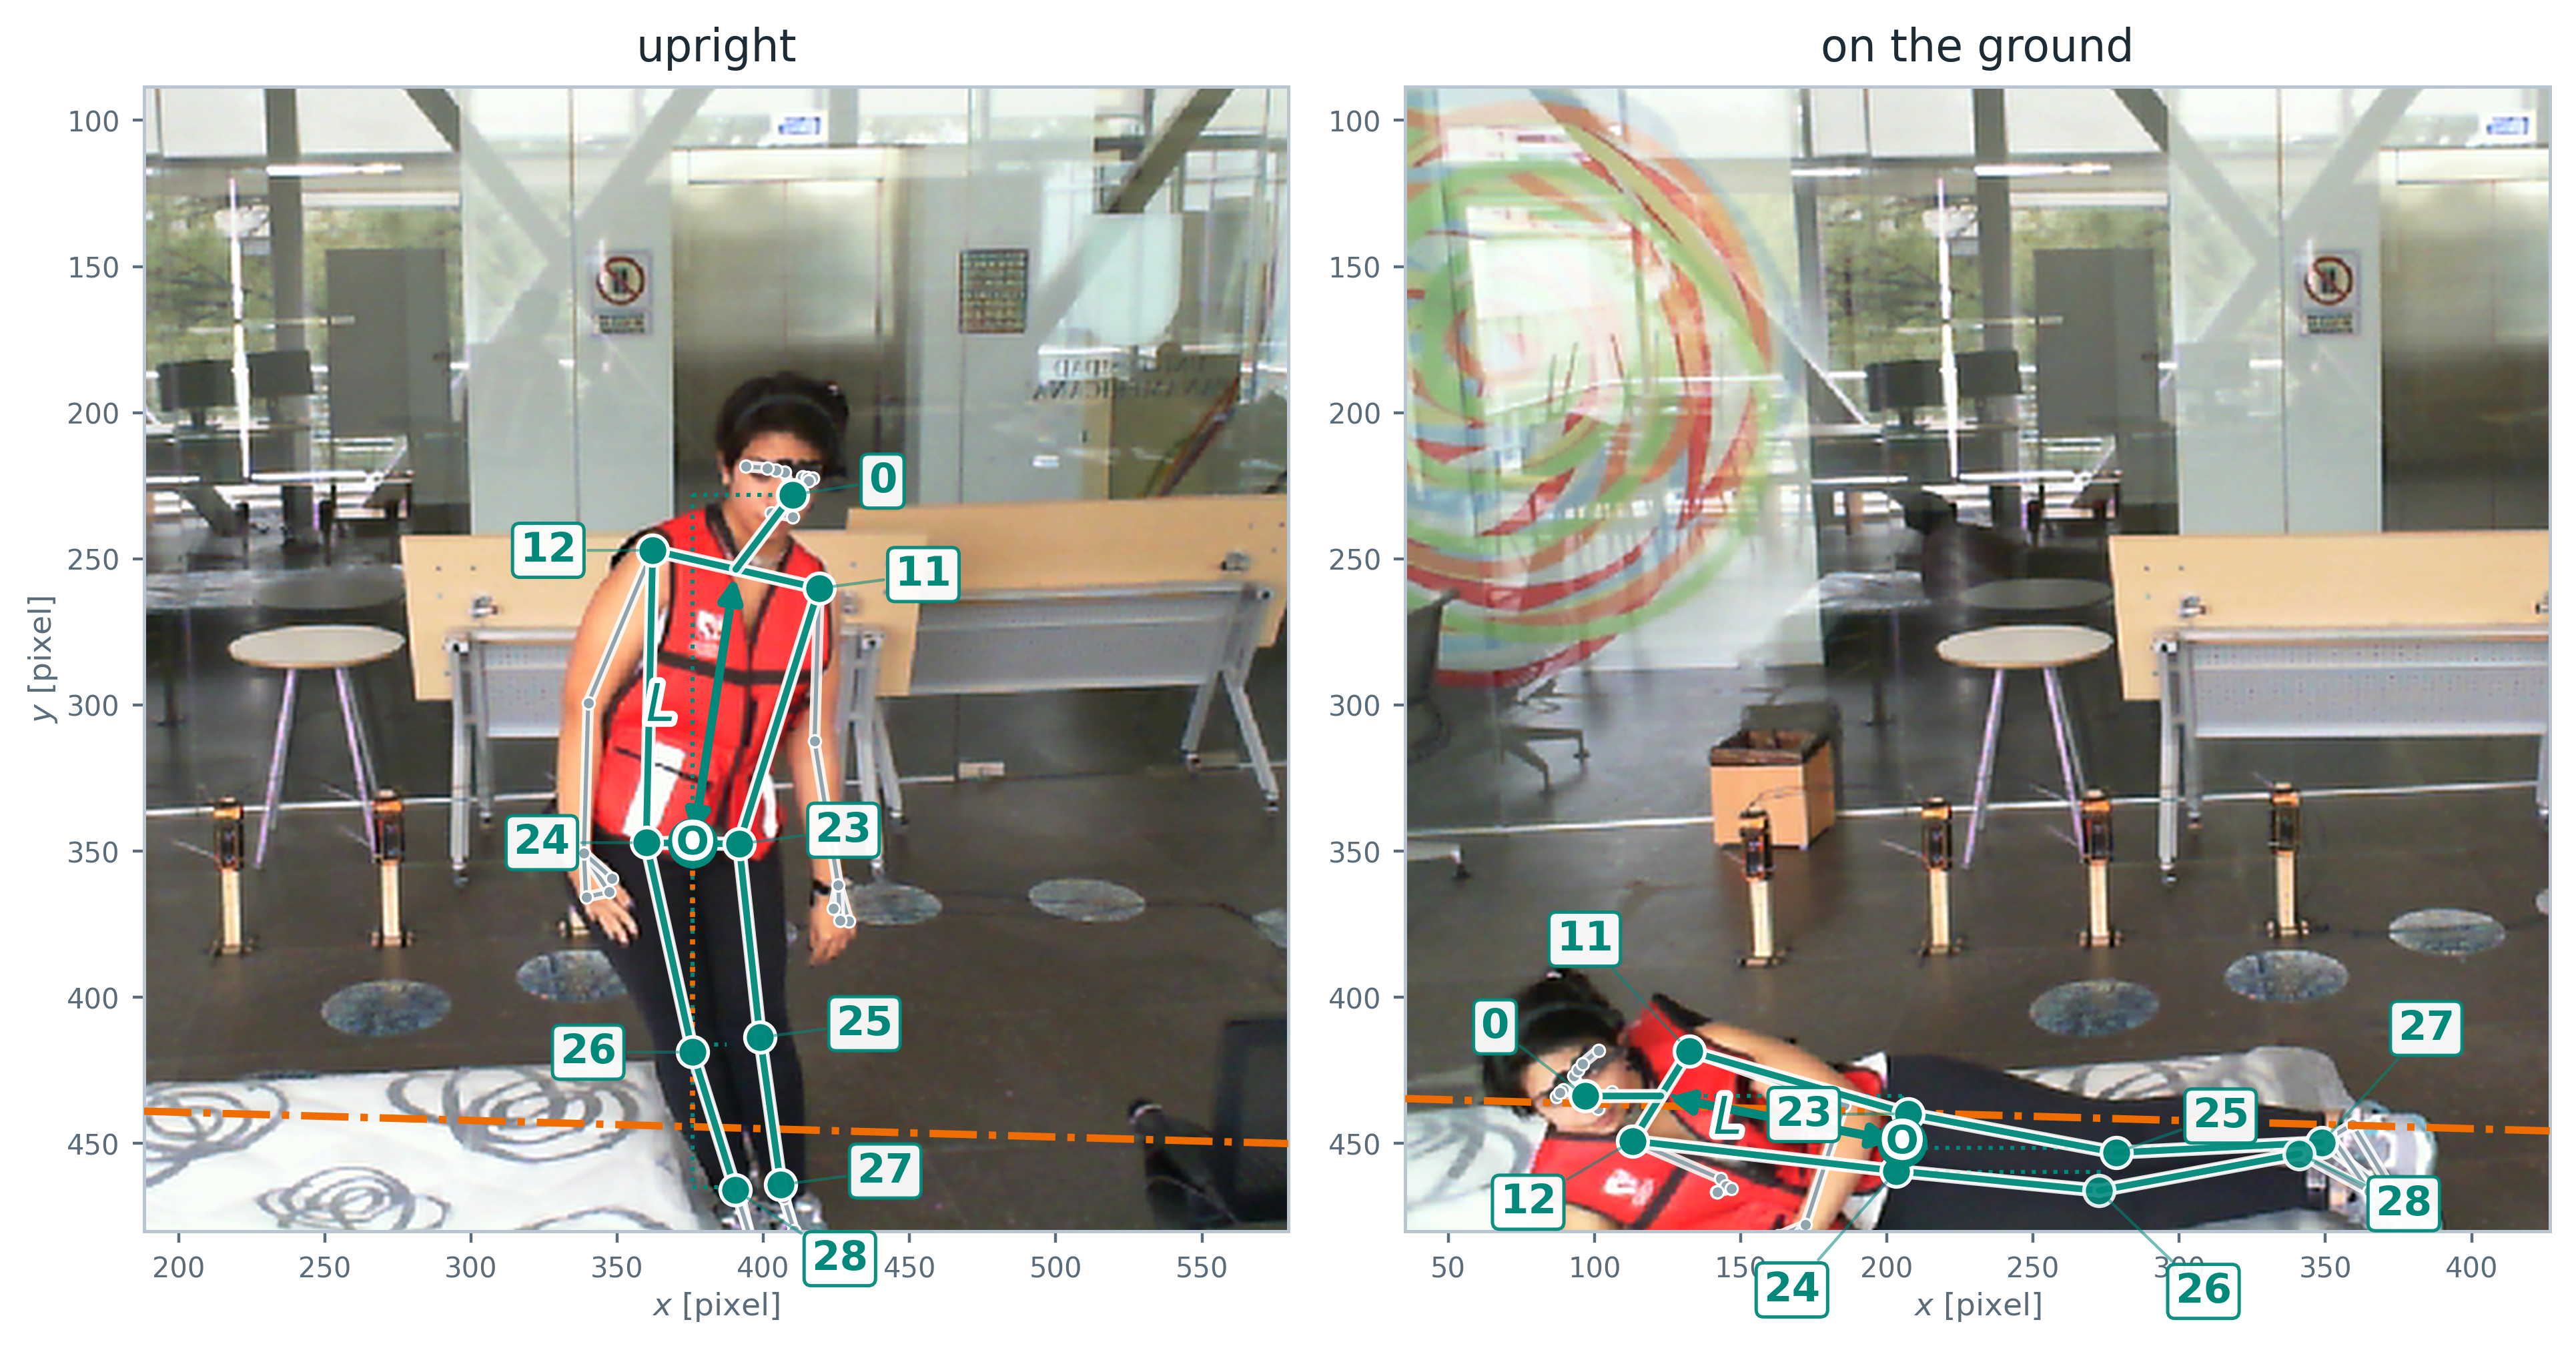
\includegraphics[width=\textwidth]{figure/fig_momenti_a3_en.png}
\caption{Representation A3 at the same two instants as
Figures~\ref{fig:momenti_a1} and~\ref{fig:momenti_a2}. The point O marks the
centre of the hips, used as the origin of the reference frame, while $L$
represents the length of the trunk used to normalise the distances.}
\label{fig:momenti_a3}
\end{figure}

The normalisation reduces the dependence on translation and scale, but does not eliminate the one due to perspective. Moreover, by referring the landmarks to the hips, the information about the absolute position of the person in the environment is lost. A person lying on the floor and one lying on a bed can generate very similar body-centric configurations. In order to recover this information, Section~\ref{sec:pavimento} will introduce the position of the hips with respect to the floor, estimated from the scene. Taken together, the three representations described provide 23 basic geometric and kinematic quantities: nine belonging to A1, five to A2 and nine to A3.

\section{Integral quantities for the description of movement}
\label{sec:integrali}

The representations described in the previous section comprise both static quantities and dynamic quantities obtained through differences between consecutive frames. As discussed in Section~\ref{sec:filtraggio}, the coordinates are estimates and show small oscillations even when the real position of the body varies little. In order to provide a description of the movement over a wider time interval, three integral quantities were introduced.

\subsection{Definition of the integral quantities}

The quantities are computed over a sliding window containing the last \(K\) frames. Denoting by
\[
W_t=\{t-K+1,\ldots,t\}
\]
the window considered, by \(\theta_t\) the orientation of the trunk and by \((x_t,y_t)\) the position of the point being followed, the following are defined:

\begin{align}
\text{escursione}_t &= \max_{\tau \in W} \theta_\tau
                     - \min_{\tau \in W} \theta_\tau
                     \label{eq:escursione}\\[4pt]
\text{percorso}_t   &= \frac{1}{s}\sum_{\tau \in W}
                       \sqrt{(x_\tau - x_{\tau-1})^2 + (y_\tau - y_{\tau-1})^2}
                     \label{eq:percorso}\\[4pt]
\text{discesa}_t    &= \frac{1}{s}\Big( y_t - \min_{\tau \in W} y_\tau \Big)
                     \label{eq:discesa}
\end{align}

The three features describe different aspects of the movement. The \emph{excursion} measures how much the orientation of the trunk varies within the window, the \emph{path} the distance covered overall by the point being followed, and the \emph{descent} how far below the highest recently observed position the current point lies.

The factor \(s\) is used to normalise the distances. For A1 it is derived from the size of the silhouette, while for A2 and A3 the length of the trunk is used. In this way the quantities depend less on the apparent size of the person in the image.

The point being followed also changes according to the representation:
\begin{itemize}
    \item A1: centroid of the set of landmarks,
    \item A2: nose in the \emph{world landmarks}.
    \item A3: centre of the hips in the image plane,
\end{itemize}

Accumulating over several samples does not eliminate the noise of the landmarks. In the path, for instance, distances that are always positive are summed, and so any oscillations may increase the distance covered rather than cancelling out. Excursion and descent can likewise be affected by outliers, since they depend on the maximum, the minimum, or both. The advantage is that they describe the movement on a wider time scale instead of depending solely on the variation between two consecutive frames. The resulting signal is therefore more regular, while remaining sensitive to the errors introduced by pose estimation.

\begin{figure}[ht]
\centering
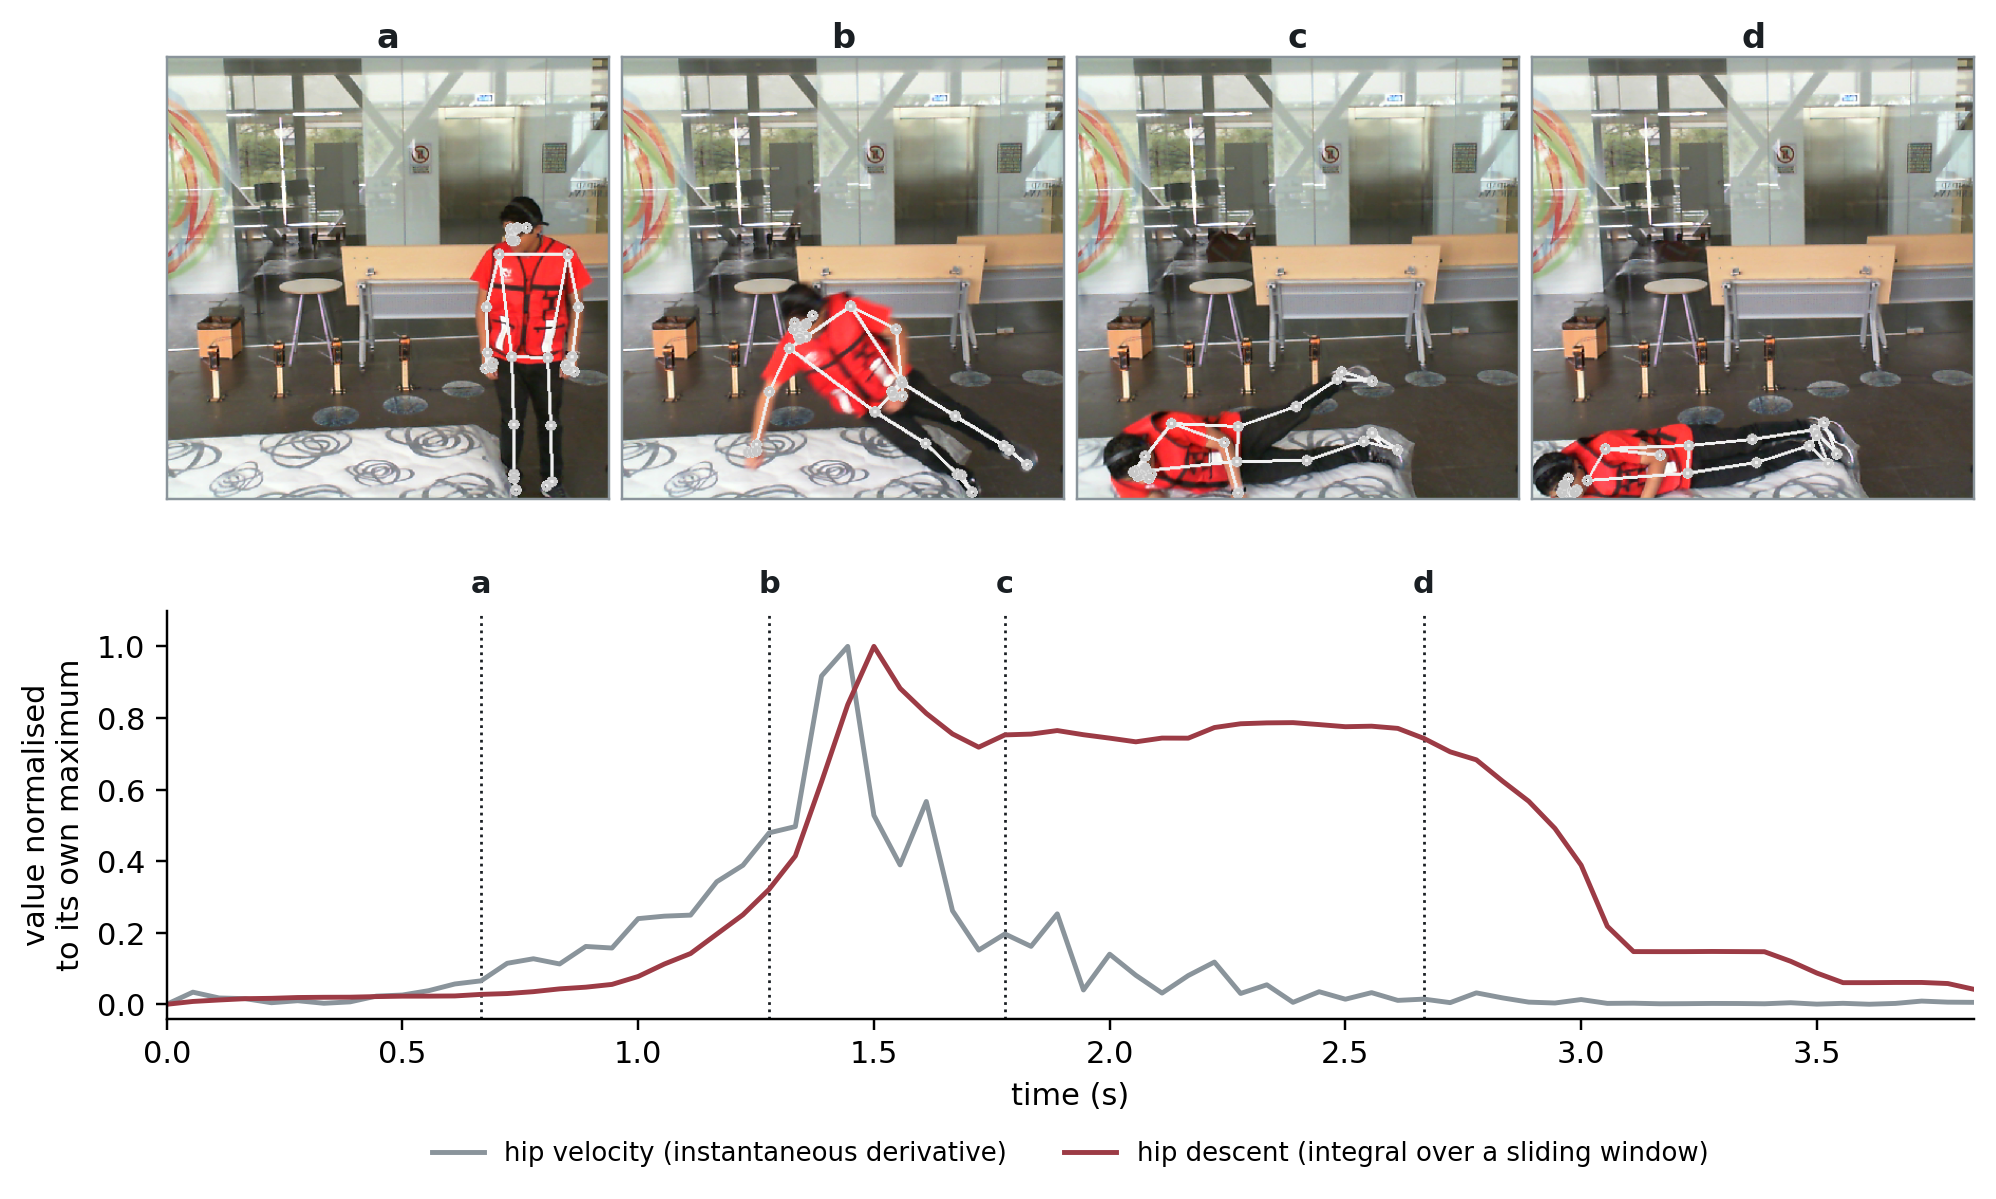
\includegraphics[width=\textwidth]{figure/fig_striscia_en.png}
\caption{Comparison between an instantaneous quantity and an integral quantity during a fall.} \label{fig:striscia}
\end{figure}

Figure~\ref{fig:striscia} shows the contrast on a single fall. The two quantities rise together and reach their maximum during the transition: the derivative is no less sensitive to the event. As soon as the body comes to rest, the velocity of the hips collapses, going from $3{,}76$ at instant (b) to $0{,}11$ at instant (d), while the accumulated descent rises to $1{,}40$ and stays there, decaying only when the accumulation window leaves the event.

\subsection{Causal computation and choice of the length $K$}

The quantities defined in Equations~\eqref{eq:escursione}--\eqref{eq:discesa} can be computed in two ways. In offline processing they could be computed by sliding a window over the whole sequence, which is already available. That solution would not, however, be directly usable on the edge device, where the frames arrive one at a time and no information later than the current instant is available.

In order to use the same logic in both conditions, the pipeline keeps a circular buffer containing the last \(K\) samples and, at every new frame, updates the three integral quantities using only the information already observed. The computation is therefore causal and is applied in the same way both during offline extraction and during execution on the device.
If the pose is lost, the buffer is reset. This prevents the accumulation from spanning an interval in which the movement of the person was not monitored. After start-up, or after a loss of the pose, the buffer must therefore fill up again before the whole expected history is available.

The length of the buffer determines how much recent movement enters the computation. With a small value a shorter interval is observed and the representation is more responsive, but little noise is attenuated. Increasing \(K\) means that a longer portion of the sequence is considered, but a brief event may end up spread over a larger number of samples. The value adopted is
\[
K=31.
\]
At the nominal frequency of 18 frames per second, 31 samples correspond to about
\[
\frac{31}{18}\simeq 1{,}72\text{ s}.
\]

\(K\) denotes, however, a number of samples and not a fixed duration. Considering the frequencies actually measured in the dataset, 31 frames cover roughly between 1,58 and 2,15~s. On the edge device, where the processing frequency may be lower, the same number of samples may therefore represent an even longer time interval. This misalignment is analysed in Chapter~\ref{cap:edge}.

The buffer moreover requires an initial warm-up period: in the first \(K\) frames after start-up the quantities do not yet have the whole history required, and the same happens after a loss of the pose, since the buffer is reinitialised. The value \(K=31\) is retained in the configuration used in the experiments. The effect of different values is assessed in the following chapters, together with the consequences for the operation of the system in a real environment.
The three quantities are computed for A1, A2 and A3. Nine are therefore added to the 23 basic geometric and kinematic quantities, bringing the overall number of candidate features to \textbf{32}.

\subsection{Assessment of temporal regularity}
\label{sec:regolarita}

In order to compare the regularity over time of the instantaneous quantities and of the integral ones, the one-step autocorrelation was measured, that is the correlation between the value of a quantity at time \(t\) and its value at the previous sample:
\[
\rho_1 = \frac{\operatorname{Cov}\big(x_t,\,x_{t-1}\big)}
              {\sigma_{x_t}\,\sigma_{x_{t-1}}}.
\]

The computation considers only pairs of consecutive samples belonging to continuous stretches in which the pose is available. If tracking is lost, the samples lying on either side of the interruption are not related to each other.

The autocorrelation describes how far the value of a quantity tends to stay similar between two consecutive samples. A high value of \(\rho_1\) indicates that the quantity tends to change more gradually, while lower values indicate more rapid variations.
This measure was used only to compare the temporal regularity of the signals. It cannot establish whether a feature is more useful for distinguishing a fall from an ordinary daily activity. The values obtained and the comparison between the two families of quantities are reported in Section~\ref{sec:autocorrelazione} of the experimental chapter.

\subsection{Robustness and limitations}
\label{sec:robustezza}

The three integral quantities nonetheless depend on the coordinates produced by the pose estimator. In order to verify how far small variations of the landmarks can affect performance, a test was carried out by adding independent Gaussian noise to the coordinates.

Denoting by \(p\) a coordinate of the landmark, the perturbed value is
\[ \tilde{p}=p+\varepsilon,
\]
with
\[ \varepsilon \sim \mathcal{N} \left(0,\left(\sigma L_{\text{tronco}}\right)^2\right),
\]
where \(L_{\text{tronco}}\) is the length of the trunk and \(\sigma\) denotes the relative intensity of the noise. The standard deviation of the noise is therefore expressed as a fraction of the length of the torso, so that the intensity of the perturbation does not depend on the size of the person in the image.
The test is repeated using
\[
\sigma \in \{0,\;0{,}005,\;0{,}010,\;0{,}020,\;0{,}040\}.
\]
For every level, three sets of features are compared: the representation without the integral quantities, the complete one with the integral quantities, and the subset selected by DTW. The results are reported in Section~\ref{sec:rumore}.

This test describes, however, only small random and independent perturbations of the coordinates. In some domestic recordings a different behaviour was also observed: in the presence of occlusions, or when the person is very close to the camera, the estimator may switch between alternative configurations of the same pose and keep the wrong configuration for several frames.

An error that is coherent over time may be interpreted by the integral quantities as real movement. The behaviour is also analysed on the domestic recordings, comparing the excursion of the trunk computed over the sliding window in sequences where the person remains still on a sofa and in sequences containing a fall. Using a time window therefore reduces the dependence on instantaneous differences, but does not eliminate the dependence on the correctness of the pose. The quantitative verification is discussed together with the noise test in Section~\ref{sec:rumore}.

\section{Estimating the height of the hips above the floor}
\label{sec:pavimento}

Representation A3 normalises every quantity with respect to the centre of the hips and to the length of the trunk. This choice reduces the dependence on the position and on the scale of the person in the image, but loses the information about their absolute position in the scene.
The limitation shows itself when similar postures occur at different heights. A person lying on a bed or on a sofa may have a body configuration very similar to that of a person who has remained on the ground after a fall. Body-centric coordinates alone describe the posture well, but cannot tell us at what height it is with respect to the environment.

In order to recover this information, a measure of the height of the hips above the floor was introduced. The feature was not part of the initial representation and was added following the checks carried out in a domestic environment. The position of the floor is not supplied manually. The frames in which the person is sufficiently upright are used. Under such conditions the lower edge of the region occupied by the body is used as an approximation of the position of the floor at the corresponding abscissa.

For every frame the pair
\[ \left( x_{\text{bacino}}, y_{\text{bordo}} \right),
\]
was collected, where \(x_{\text{bacino}}\) is the horizontal coordinate of the centre of the hips and \(y_{\text{bordo}}\) the vertical coordinate of the lower edge of the body. Starting from these points, the line
\[
y_{\text{pav}}(x) = a\,x + c,
\]
is estimated by least squares, representing the position of the floor in the image plane. Using a line instead of a constant vertical level captures the apparent variation in the position of the floor due to perspective. Once the reference has been obtained, the height of the hips is computed as:
\[
h_{\text{pav}} =
\frac{y_{\text{pav}}(x_{\text{bacino}}) - y_{\text{bacino}}}
                      {L_{\text{tronco}}},
\]
where $L_{\text{tronco}}$ is the length of the trunk already used in representation A3.

\begin{figure}[ht]
\centering
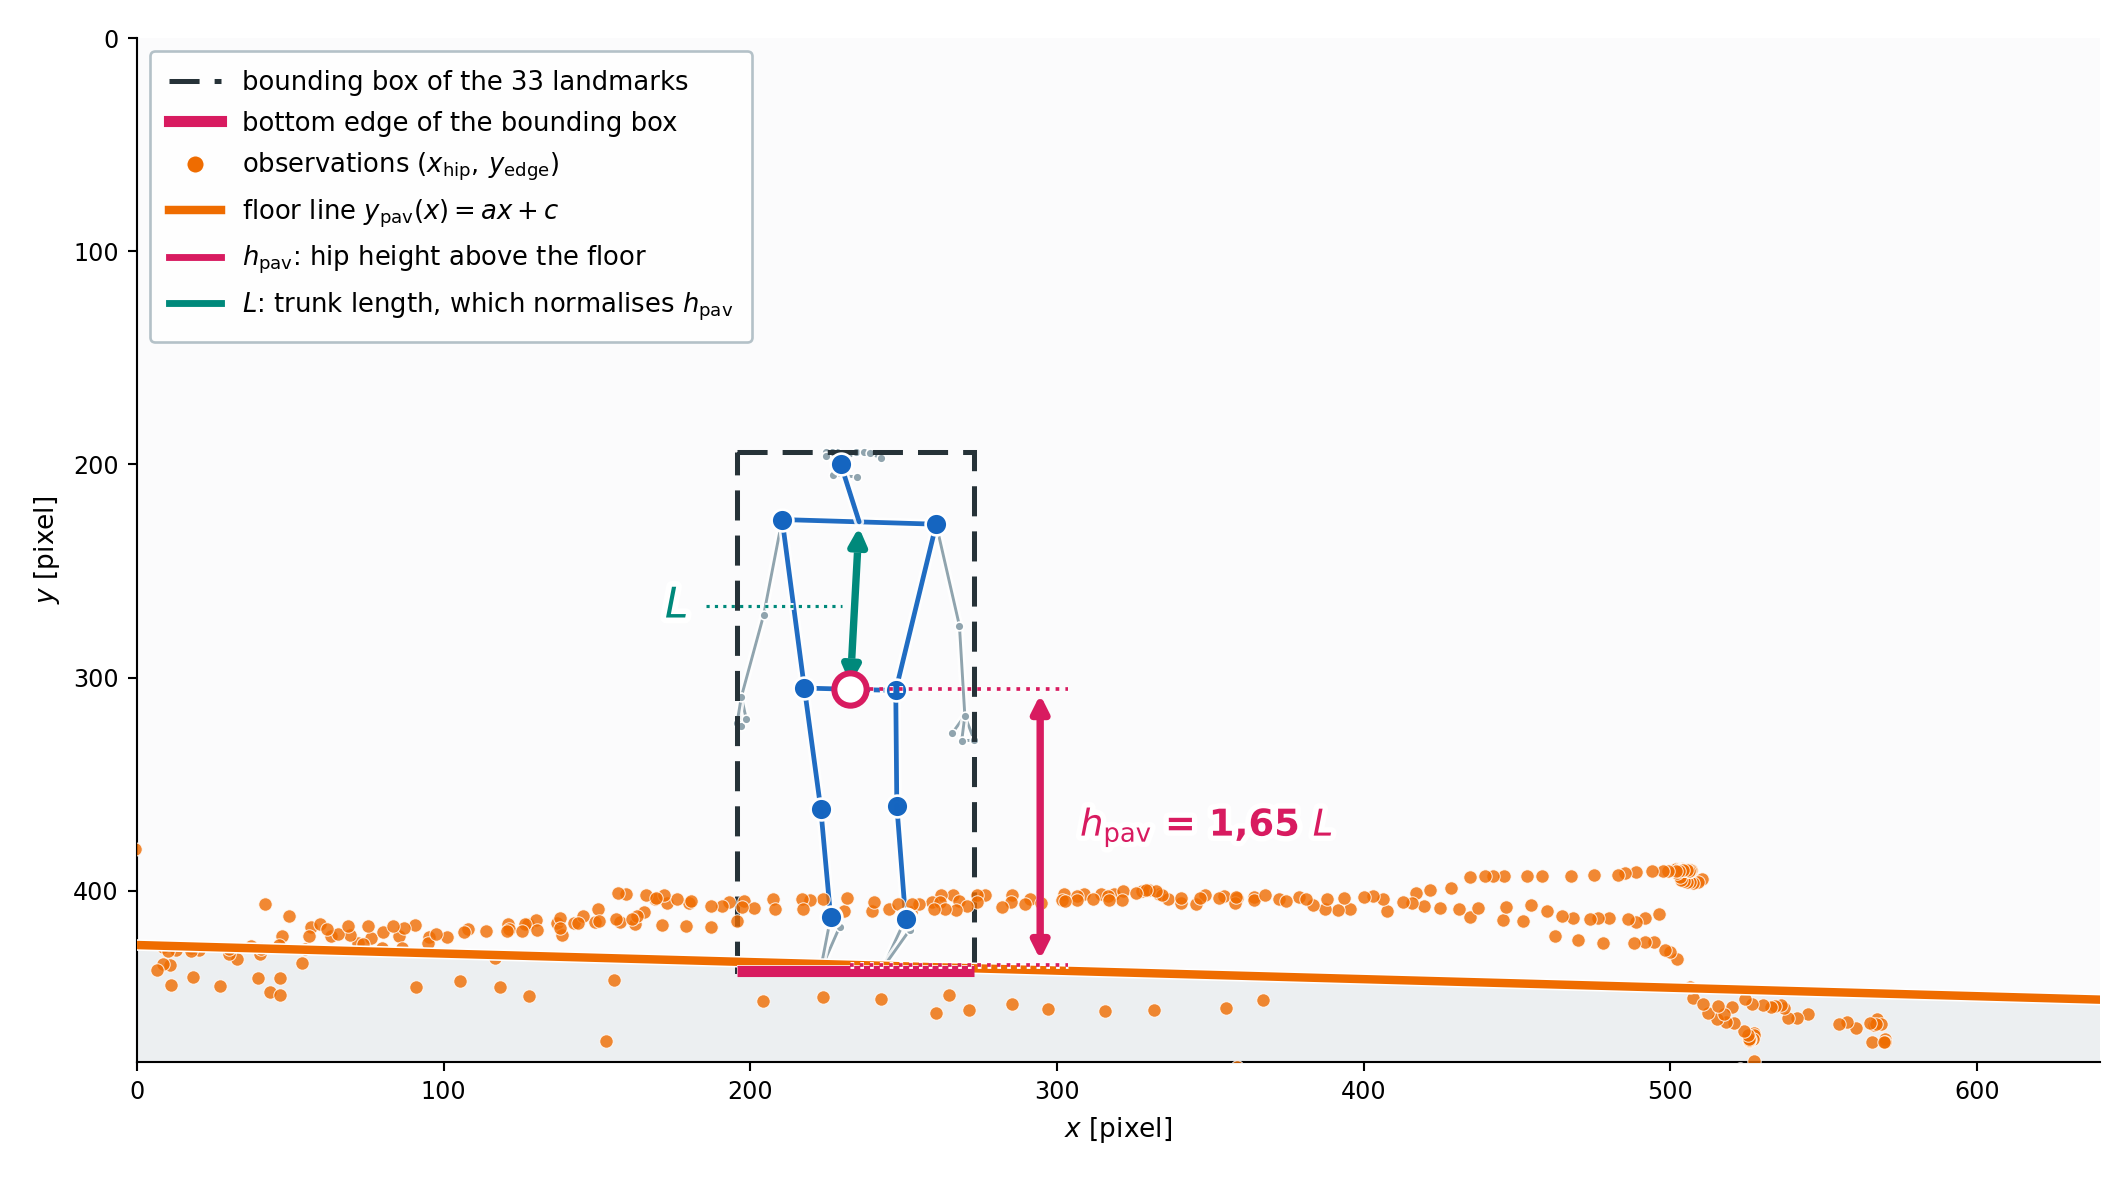
\includegraphics[width=\textwidth]{figure/fig_pavimento_en.png}
\caption{Estimating the height of the hips above the floor. From the frames
in which the person is standing, the points
\((x_{\text{bacino}}, y_{\text{bordo}})\) are collected and used to estimate the
floor line \(y_{\text{pav}}(x)\). The height \(h_{\text{pav}}\) is then computed
as the vertical distance between the centre of the hips and the floor line,
normalised with respect to the length of the trunk.}
\label{fig:pavimento}
\end{figure}

Dividing by \(L_{\text{tronco}}\) makes the quantity dimensionless and reduces the effect of the scale at which the person appears in the image. The parameters \(a\) and \(c\) remain instead tied to the individual installation, because they describe the position of the floor as observed from that camera.

The estimate uses the lower edge of the box containing all 33 landmarks, and some of them may be estimated outside the image when part of the body is not fully visible. The phenomenon concerns the extremities above all: in the frames examined, the tip of the foot is estimated below the lower edge in 48\% of cases and the wrist in 32\%.
In one recording used to check the effect on the estimate, 17,8\% of the observations exceed the lower limit of the image, with a median excess of 60 pixels over a height of 480. Repeating the computation after clipping the vertical coordinates to the height of the image, the estimated line shifts by 12 pixels, about one sixth of the length of the trunk in the sequence considered. Fitting over several observations reduces the effect of individual outliers, but does not remove it altogether, and it must be declared as a downward bias of the estimate.

The viewpoint of the camera also affects the measurement. For \(h_{\text{pav}}\) to be informative, the vertical displacement of the person must produce a visible variation in the image plane. A lateral view, placed roughly at chest height, meets this condition better than a strongly raised view. The dependence was verified by computing \(h_{\text{pav}}\) separately for the two cameras of the dataset and comparing, for each view, the distributions obtained in the fall frames and in the frames of daily activity. The results are reported in Section~\ref{sec:viewpoint}.

Finally, the floor line requires a certain number of observations of the person in an upright position. At system start-up the reference is therefore not immediately available and, until enough samples have been collected, \(h_{\text{pav}}\) cannot be used. The effect of this initial phase is verified on the domestic recordings in Chapter~\ref{cap:edge}.
One possible alternative would be to calibrate the floor once during installation and store \(a\) and \(c\) together with the configuration of the camera. This solution would avoid rebuilding the reference at every new run, but it was not implemented in the system developed, because a stored line remains valid only as long as the camera is not moved, whereas the online estimate adapts by itself.

In what follows, A3 denotes the basic body-centric representation, A3h the same representation with the addition of the height of the hips above the floor, and A3i the extension with the three integral quantities. The two extensions are independent and can also be used together.
With the addition of the height above the floor, the overall number of candidate features goes from 32 to \textbf{33}.

\section{Selecting the quantities by means of \emph{Dynamic Time Warping}}
\label{sec:dtw}

The 33 candidate features are not necessarily all useful for distinguishing a fall from daily activities. Before training, a preselection was therefore carried out by directly comparing the time series produced by the different features.

For this purpose \emph{Dynamic Time Warping} (DTW) was used, a technique which, unlike a distance computed point by point such as the Euclidean one, makes it possible to deform the time axis locally so as to align curves that describe similar shapes even when they evolve at different speeds, and which seeks the alignment producing the lowest overall cost. Two curves with a similar shape can thus turn out to be close even when the same change does not occur at the same instant.

In the present work the DTW is not used by the classifier, but only as an analysis tool to assess the separability of the features. The idea is that a useful quantity should produce similar trajectories among examples of the same class and, at the same time, different ones between falls and daily activities.
\begin{figure}[htbp]
    \centering
    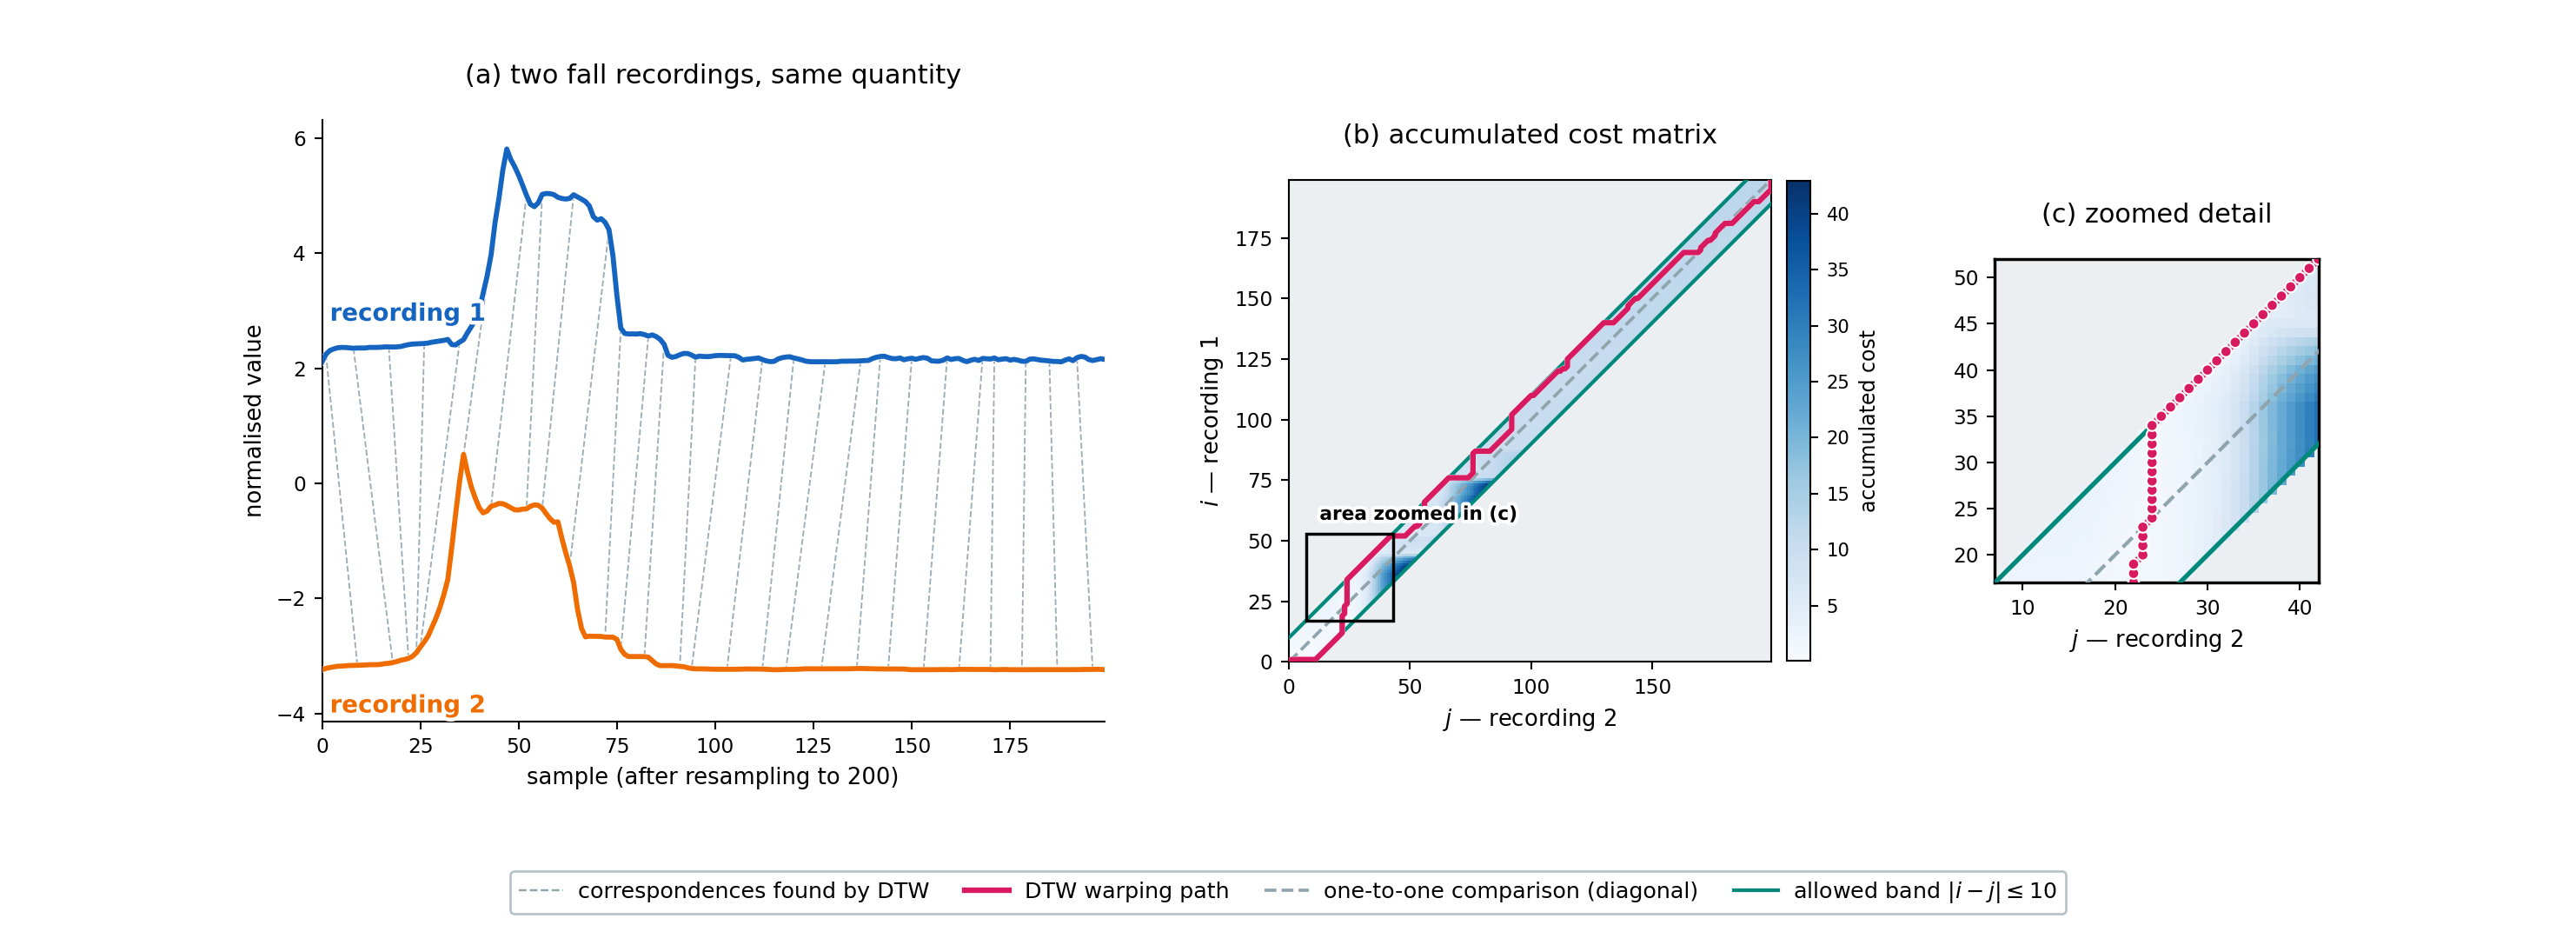
\includegraphics[width=\linewidth]{figure/fig_dtw_spiegazione_en.png}
    \caption{Example of alignment by DTW and of the band constraint used in the selection procedure.}
    \label{fig:dtw_allineamento}
\end{figure}

\subsection{Normalisation and resampling}

Before the comparison, every time series is normalised separately to zero mean and unit standard deviation:
\[
\tilde{x}_t = \frac{x_t-\mu_x}{\sigma_x}.
\]
This choice makes it possible to compare features with different scales and units of measurement: some are angles, others velocities, others still dimensionless ratios. Without this operation the distance would also be influenced by the numerical magnitude of the quantity, whereas at this stage what matters above all is the shape of the curve.

The fall recordings and those relating to daily activities have very different durations, about 180 and 820 frames respectively. Comparing such different sequences directly would require a very wide alignment band precisely in the comparison between the two classes.
In order to preserve the same meaning for the alignment constraint, after normalisation all the curves are resampled to a common length of 200 samples. This operation is used only in the DTW analysis and does not alter the data subsequently supplied to the classifier.

\subsection{Separability score and selection}

The temporal deformation allowed by the DTW is limited by imposing
\[
|i-j|\leq 10,
\]
where $i$ and $j$ are the indices of the samples in the two sequences. Small temporal shifts are thus admitted, while at the same time parts of the two curves that are too far apart are prevented from being matched. For each quantity three families of distances are computed:
\begin{itemize}
\item \(D_{FF}\), between pairs of fall recordings;
\item \(D_{AA}\), between pairs of daily activities;
\item \(D_{FA}\), between a fall and a daily activity.
\end{itemize}

A discriminative quantity should produce small distances within the same class and larger ones between the two classes. Denoting by
\[
\mu_{\mathrm{intra}}=\frac{\mu_{FF}+\mu_{AA}}{2},
\]
the mean intra-class distance, the separability score is defined as
\[
S=
\frac{\mu_{FA}}
     {\mu_{\mathrm{intra}}+\varepsilon},
\]
where \(\varepsilon\) prevents division by zero. A value close to one indicates that the inter-class distances are similar to the intra-class one, while larger values indicate a sharper difference.

UP-Fall observes the same events from two different viewpoints. The initial analysis computed a single score, considering the recordings of the two cameras together. That choice may, however, favour a feature that is highly discriminative in one view and poorly informative in the other. The score is therefore computed separately for each view, and for the selection
\[
S_{\text{robusto}} = \min\big(S_{\text{cam}_1},\ S_{\text{cam}_2}\big).
\]
is considered.

The lower value is chosen, rather than the mean, so as to prevent a feature that is effective from one view alone from nonetheless obtaining a high score. The effect of the viewpoint on the values obtained is analysed in Section~\ref{sec:viewpoint}.

The DTW, however, assesses every feature separately, and two quantities may both obtain a good score while describing almost the same information. In order to limit this redundancy, the features are ordered according to \(S_{\text{robusto}}\) and considered in sequence. A new quantity is retained only if its absolute correlation with all those already selected satisfies
\[
|\rho|<0{,}85.
\]

The correlation is computed only on the frames with a valid pose, so that the values inserted where the pose is missing do not create correlations that have nothing to do with the content of the features.
Four features are excluded from the subset for precisely this reason, and are reported in Table~\ref{tab:ridondanti}.

\begin{table}[ht]
\centering
\caption{Quantities excluded for redundancy, with the feature already selected with respect to which the correlation threshold is exceeded.}
\label{tab:ridondanti}
\begin{tabular}{@{}llc@{}}
\toprule
\textbf{Excluded} & \textbf{Redundant with} & \textbf{\(|\rho|\)} \\
\midrule
\texttt{A2\_angolo\_tronco}    & \texttt{A2\_testa\_rel\_y}    & 0,97 \\
\texttt{A3\_testa\_rel\_y}     & \texttt{A2\_testa\_rel\_y}    & 0,98 \\
\texttt{A2\_escursione}        & \texttt{A3\_escursione}       & 0,86 \\
\texttt{A3\_ginocchia\_rel\_y} & \texttt{A3\_caviglie\_rel\_y} & 0,93 \\
\bottomrule
\end{tabular}
\end{table}

The procedure leads to the selection of 12 of the 33 candidate quantities. In decreasing order of $S_{\mathrm{robusto}}$, the features selected are
\texttt{A2\_testa\_rel\_y}, \texttt{A2\_discesa},
\texttt{A2\_percorso}, \texttt{A1\_discesa}, \texttt{A3\_discesa},
\texttt{A3\_escursione}, \texttt{A3\_caviglie\_rel\_y}, \texttt{A3\_percorso},
\texttt{A3\_hip\_vel}, \texttt{A3\_testa\_vel\_rel}, \texttt{A1\_percorso} and
\texttt{A1\_escursione}.

The mean correlation among them is \(0{,}435\). The subset comprises features coming from all three representations, and eight of the twelve are integral quantities. A particular case is that of the height of the hips above the floor. The feature obtains \(1{,}541\) on the lateral view, the second highest score among the 33, and \(1{,}124\) on the raised one. The gap, \(0{,}417\), is the largest of the whole set.

The minimum between the two views therefore places it twenty-first, and the selection excludes it. The result is consistent with the aim of the criterion: to prevent quantities whose effectiveness depends heavily on the position of the camera from being favoured. The acquisition protocol envisaged for the installed system does, however, use a lateral view, in which the height above the floor shows its most favourable behaviour. For this reason a second configuration is also analysed, denoted by \textbf{DTWH}, obtained by adding the height of the hips above the floor to the 12 features selected by DTW.

\begin{table}[htbp]
\centering
\caption{Abbreviations used to denote the main feature configurations.}
\label{tab:sigle}
\begin{tabular}{@{}llc@{}}
\toprule
\textbf{Abbreviation} & \textbf{What it contains} & \textbf{No.} \\
\midrule
A1, A2, A3 & the set of the three representations, integral quantities included & 32 \\
A3base & basic A3 representation & 9 \\
A3h & A3 with the height of the hips above the floor & 10 \\
A3i & A3 with the three integral quantities & 12 \\
\textbf{DTW} & \textbf{subset obtained from the automatic selection} & \textbf{12} \\
DTWH & DTW plus the height above the floor & 13 \\
\bottomrule
\end{tabular}
\end{table}

One last point concerns the relationship between this selection and the \emph{leave-one-subject-out} protocol. In a LOSO evaluation, the subject used as test should take part in no operation that derives information from the data, feature selection included. In the pipeline used, the DTW selection was instead carried out once over the whole dataset before the LOSO, and the same 12 features were subsequently used in every fold. The subject left out therefore contributed indirectly to the choice of the features. This introduces a form of \emph{data leakage} that must be borne in mind when reading the results.

In order to quantify its effect, in Chapter~\ref{cap:sperimentale} the procedure is repeated separately for each fold, excluding the test subject every time and comparing the subset obtained with the one adopted. The normalisation described at the beginning of this section is the one internal to the DTW analysis, and is applied separately to the individual curves. It is not to be confused with the normalisation of the data supplied to the classifiers, which is instead estimated within each fold on the training data alone, as described in Section~\ref{sec:classificatori}.

\section{Construction of the temporal windows}
\label{sec:finestre}

The classifier receives as input sequences of features organised into temporal windows. The same body configuration may appear in different activities, whereas the way the pose changes over time supplies the information that distinguishes a fall from an ordinary daily activity.
Denoting by $f_t$ the feature vector at sample $t$, a window of length \(L\) is defined as
\[
X_t = [\,f_t, f_{t+1},\dots, f_{t+L-1}\,].
\]

Before the windows are built, the sequence extracted at about 18 fps is subsampled by taking one sample in two, so that the classifier works at a nominal frequency of about 9 samples per second. In the configuration used, a length $L=22$ is chosen which, at that frequency, corresponds to about
\[
\frac{22}{9}\simeq 2{,}44\text{ s}.
\]

The choice of length is a compromise. A window that is too short observes only part of the movement and may not contain enough context to distinguish a fall from a rapid activity; a very long window includes more frames that do not belong to the phase of interest and increases the time needed for a sequence to be complete.

The value of 22 samples was inherited from an earlier configuration that used 45 samples at 18 fps, thus preserving a similar duration. Windows of 28, 36 and 44 samples were also considered, corresponding to intervals between about $2{,}4$ and $4{,}9$ s. The laboratory $F_2$ improves systematically as the length increases, but in the final configuration $L=22$ was retained in order to limit latency. The comparison between the different lengths is reported in Chapter~\ref{cap:sperimentale}. The windows are built with a stride of two samples: two consecutive windows therefore share 20 samples out of 22 and are strongly overlapping. This choice reduces the risk that a fall falls across two windows without being sufficiently represented in either. Neighbouring windows cannot, however, be considered independent observations, an aspect that is taken into account when separating training data from test data.

Subsampling and the stride of the window denote two different operations. The first establishes which samples enter the classifier; the second establishes how often a new window is built. The features are computed before subsampling: a dynamic quantity contained in a sample therefore retains the value obtained during extraction on the original sequence, and subsampling comes into play only in the subsequent construction of the windows. Finally, a window is built only within a continuous stretch with a valid pose. If the estimator loses the person, the sequence is interrupted and construction resumes only when a sufficient number of consecutive frames is available again. In this way a window never contains frames belonging to two intervals separated by a loss of tracking.

\section{Definition of the task and assignment of the label}
\label{sec:compito}

A fall comprises two distinct moments: the movement by which the person loses their balance and reaches the ground, and the subsequent state in which they remain on the ground. The UP-Fall recordings were observed and annotated manually at frame level, distinguishing three phases:
\begin{itemize}
    \item \textbf{ordinary activity}, corresponding to the phase preceding the loss of balance;
    \item \textbf{transition}, from the loss of balance until arrival on the ground;
    \item \textbf{post-fall state}, in which the person remains on the ground.
\end{itemize}

The labels $0$, $1$ and $2$ were associated with the three conditions respectively. These annotations constitute the frame-level reference from which the labels of the temporal windows are derived. The three phases have different durations. Considering the 50 fall recordings of Camera~1, relating to the ten subjects used, the values reported in Table~\ref{tab:durate_fasi} are obtained.

\begin{table}[ht]
\centering
\caption{Duration of the three phases in the UP-Fall fall recordings considered for Camera~1.}
\label{tab:durate_fasi}
\begin{tabular}{lccc}
\hline
\textbf{Phase} & \textbf{Median} & \textbf{10\% decile} & \textbf{90\% decile} \\
\hline
Before the fall & 0,94 s & --- & --- \\
Transition & 3,11 s & 2,05 s & 3,94 s \\
Post-fall state & 5,97 s & 4,82 s & 6,89 s \\
\hline
\end{tabular}
\end{table}

The transition therefore lasts a little over three seconds, while the post-fall state occupies on average an even longer interval. Distinguishing the two phases separates the event of falling from the condition that follows it, and the distinction is not academic: from an applicative point of view, including the post-fall state as well would be the natural choice, since remaining on the ground is the condition that matters in monitoring and lasts far longer than the dynamic phase.

The problem emerges when one considers the daily activities that produce a similar final configuration. A person may find themselves in a horizontal position without having fallen, and UP-Fall contains the activity \emph{laying}, in which the subject lies down voluntarily: it comprises 20.980 frames, about 18\% of the dataset, labelled as daily activity, against 10.524 belonging to the post-fall state.
For this reason the two phases are kept separate in the reference ground truth. In the final configuration of the system the transition is used as the main positive event, while the post-fall state is kept distinct, both in order to build the window labels correctly and in order to compare different formulations of the problem.

Once the three phases have been defined at frame level, it is necessary to establish how to transfer these annotations to the temporal windows. A window may comprise samples belonging to different phases and cannot therefore be labelled on the basis of a single frame.

For the construction of the main labels it was decided to take into account the temporal arrangement of the frames within the window as well. A simple total count assigns the same weight to samples spread along the whole sequence and to samples concentrated in the same interval. For this reason a $K$-of-$M$ criterion was adopted. Denoting by $m_t$ a binary variable equal to one when the frame belongs to the phase considered,
\[
\max_i \sum_{t=i}^{i+M-1} m_t \geq K.
\]
The phase is considered present when at least $K$ frames associated with it lie within a local interval of $M$ samples.
For the transition $K=5, \qquad M=8$ are used, while for the post-fall state $K = 10, \qquad M = 15$. These values form part of the preprocessing procedure and were not obtained by directly optimising the performance of the classifier.

Starting from the presence of the transition and of the post-fall state, three formulations for training were considered:
\begin{itemize}
\item \textbf{discard}: the transition constitutes the positive class, while the windows belonging exclusively to the post-fall state are excluded from training;
\item \textbf{fall}: transition and post-fall state are both considered positive;
\item \textbf{three classes}: ordinary activity, transition and post-fall state are kept as separate classes. \end{itemize}

The three formulations therefore use the labels (0), (1) and (2) defined at frame level and the (K)-of-(M) criterion described above. In order to keep the same verification set, two labels are associated with every window. The first, $y_{\text{train}}$, depends on the formulation used during training. In the \textbf{discard} mode, the windows belonging exclusively to the post-fall state are kept in the dataset but marked with
\[
y_{\text{train}}=-1,
\]
and therefore take no part in training.

The second label, denoted by $y_{\text{allarme}}$, is instead used for the common evaluation and equals one when the transition or the post-fall state is present in the window. In this way the different formulations can be evaluated on the same set of windows.

As additional information, the annotations of \emph{OmniFall}~\cite{SN} were also used, which reannotates several fall detection datasets, among them UP-Fall, distinguishing in particular:
\begin{itemize}
    \item \texttt{fall}, relating to the fall event;
    \item \texttt{fallen}, relating to the state following the fall;
    \item \texttt{lie\_down}, relating to lying down intentionally;
    \item \texttt{lying}, relating to the subsequent lying position.
\end{itemize}

These annotations were not used to build the labels (0), (1) and (2). They were added afterwards to the features already extracted, converting the time intervals of OmniFall into the corresponding frame intervals at the nominal frequency of 18 fps. By this procedure it was possible to associate an OmniFall label with 98,5\% of the frames.

The three formulations just described must, however, be distinguished from the three tasks \emph{event}, \emph{state} and \emph{alarm} analysed in Chapter~\ref{cap:sperimentale}, because those of the present chapter use the labels (0/1/2) and the local (K)-of-(M) criterion, whereas the three tasks of the experimental chapter are built on the OmniFall classes and consider a class present when at least five of its frames appear in the window, irrespective of their temporal arrangement. The correspondence between the two sets is therefore only partial. \emph{Event} treats as positive the same phase as the \textbf{discard} mode, but treats windows of post-fall state alone as negative instead of excluding them from training. \emph{Alarm} coincides instead with \textbf{fall} in the definition of the positive class. The task \emph{state} has no counterpart among the three formulations of the present chapter, while the formulation \textbf{three classes} has no counterpart among the three tasks based on OmniFall.

\section{Classifiers and training}
\label{sec:classificatori}

The preceding sections lead from the frame to a window made of 22 samples and 12 features. It remains to be established how to use this sequence in the three training formulations defined in Section~\ref{sec:compito}.
Six architectures are compared in this work: Random Forest, LSTM, GRU, 1D CNN, Transformer and a graph network. The choice comprises models that are very different from one another, but the comparison is built so as to keep the other elements of the pipeline unchanged. The architectures therefore use the same representation, the same LOSO folds and the same decision rule.

The comparison is not meant to establish which family is the best in absolute terms. From one study to another, besides the classifier, the dataset, features, preprocessing, data split and decision threshold usually change as well, and a difference in performance may depend on any one of these. Keeping them fixed allows the differences observed to be attributed to the architecture of the classifier. For LSTM, GRU, 1D CNN, Transformer and the graph network the input keeps the shape $22 \times 12$, where the 22 rows correspond to the samples of the temporal window and the 12 columns to the selected features.

The Random Forest is instead used as a non-sequential reference, and serves to verify how much the architecture really weighs at fixed representation: if a model that does not follow the temporal order obtains results similar to those of a recurrent network, the advantage of modelling the sequence explicitly is limited under the conditions considered.
For each of the 12 features, mean, standard deviation, minimum, maximum, first and last sample are computed, producing $12\times6=72$ values. The first and last sample are there because without them the summary would preserve no direction, and a fall and a getting-up would turn out identical.
The configurations used are reported in Table~\ref{tab:modelli}.

\begin{table}[htbp]
\centering
\caption{Architectures used and their complexity. For the Random Forest
the value reported is the overall number of nodes of the trees, which is not a
parameter learnt by gradient descent but is what determines its
occupation in memory.}
\label{tab:modelli}
\begin{tabular}{@{}p{2.2cm}p{8.8cm}r@{}}
\toprule
\textbf{Model} & \textbf{Architecture} & \textbf{Parameters} \\
\midrule
GRU & two recurrent layers of 64 and 32 units, with dropout of 0,3 & 24.483 \\
LSTM & two recurrent layers of 64 and 32 units, with dropout of 0,3 & 32.227 \\
1D CNN & two temporal convolutional blocks with 64 and 128 filters, kernel of size 5, batch normalisation, subsampling by a factor of 2 and dropout of 0,3; final global average pooling & 46.147 \\
Transformer & projection to 64 dimensions, learnt positional encoding, one self-attention block with 4 heads, feed-forward layer of 128 units and global average pooling & 34.499 \\
GNN & two spatio-temporal blocks with learnt adjacency among 12 nodes, \(1\times1\) convolution with 32 channels, temporal convolution with kernel 5 and batch normalisation & 12.323 \\
Random Forest & 50 trees with no preset depth limit, trained on the 72 values derived from each window & 12.928 nodes \\
\bottomrule
\end{tabular}
\end{table}

GRU and LSTM have the same general structure and differ only in the type of recurrent cell. For the same number of units, the GRU uses fewer parameters. The 1D CNN instead processes the window by means of convolutions along the temporal dimension, while the Transformer uses a self-attention mechanism with positional encoding.

In the graph network, in order to keep the representation consistent with that of the other classifiers, the nodes are not the anatomical joints but the twelve input features, and the relations among them are learnt during training. The results of the GNN therefore refer to this configuration and do not constitute a general assessment of graph networks applied directly to the human skeleton.

The same training protocol, reported in Table~\ref{tab:addestramento}, is used for the five neural networks.

\begin{table}[htbp]
\centering
\caption{Protocol used for training the neural networks.}
\label{tab:addestramento}
\begin{tabular}{@{}p{4.6cm}p{9.0cm}@{}}
\toprule
\textbf{Element} & \textbf{Value} \\
\midrule
Input & \(22\times12\): 22 samples and 12 features \\
Output & distribution over 2 or 3 classes, according to the training formulation \\
Loss function & categorical cross-entropy \\
Class weights & inversely proportional to the frequency of the classes \\
Optimiser & Adam, initial learning rate \(10^{-3}\) \\
Epochs & at most 40 \\
Batch size & 16 \\
Early stopping & area under the curve of the \emph{alarm probability} on the validation set, patience of 8 epochs and restoration of the best weights \\
Learning-rate reduction & factor \(0{,}5\) after 4 epochs without improvement, down to a minimum of \(10^{-5}\) \\
Random seed & 42 \\
Repetitions & one per fold \\
\bottomrule
\end{tabular}
\end{table}

The decision threshold is kept fixed at
\[
\tau = 0{,}50,
\]
for all the architectures and for all the folds. The networks always produce a \emph{softmax} distribution, even in the binary case. In this way the alarm probability is derived in the same way for all the training formulations. In the binary case two classes are considered, whereas in the three-class formulation ordinary activity, transition and post-fall state are kept separate.

The Random Forest does not use the training procedure of Table~\ref{tab:addestramento}. The model is trained once for each fold using 50 trees and unlimited depth.
The hyperparameters of the models reported in Tables~\ref{tab:modelli} and~\ref{tab:addestramento} were not optimised separately on the test folds. The random seed is fixed at 42 before each model is built, and every architecture is trained only once per fold. Consequently, the dispersion reported in the results measures the variability among the subjects left out in the different LOSO folds, and not the variability due to different initialisations of the same model.

One last point concerns the operations that derive information from the data. In a LOSO protocol the subject used for the test should contribute to none of these operations.
The normalisation supplied to the classifiers is estimated within each fold using only the training data, and is then applied unchanged to the validation and test data. The threshold and the hyperparameters of the models do not depend on the test subject either, because they are kept fixed.

As discussed in Section~\ref{sec:dtw}, feature selection by DTW was applied once to the whole dataset before the LOSO, and the same 12 features were then used in every fold. The value \(K=31\) of the integral quantities was likewise chosen after a check that involved data subsequently used in the evaluation. Both aspects are therefore regarded as limitations of the protocol.

In order to assess their effect, the two procedures were repeated excluding the test subject each time. The checks, reported in Chapter~\ref{cap:sperimentale}, are however different: in the case of the DTW, the features selected within each fold are compared with those adopted in the main configuration, whereas for (K) the performance obtained is compared directly. In this second case the check moreover shows that the initial choice of (K=31) did not increase performance with respect to the selection carried out within the individual folds.

\section{From classifier output to alarm event}
\label{sec:allarme}

The classifier produces one decision per window, whereas the installed system must generate alarm events. The two things do not coincide: the windows are strongly overlapping, and a single fall may therefore produce several consecutive positive predictions.

In order to use the same rule across the different formulations of the problem, an alarm score was defined from the output of the classifier. In the binary case it coincides with the probability of the positive class; in the three-class case it corresponds to the overall probability of not belonging to the normal class, that is
\[ p_{\mathrm{allarme}} = 1-p_{\mathrm{normale}}. \]
A window is considered positive when
\[ p_{\mathrm{allarme}} \geq 0{,}50. \]

A single positive window does not, however, produce an alarm. The alert is generated only when five consecutive windows turn out positive. If a window drops below the threshold before that number is reached, the count is reset. The condition can therefore be written as a persistence of five consecutive positive decisions.

The alarm is raised at the moment the fifth consecutive positive window is observed. The four preceding windows are needed in order to verify the persistence and cannot therefore be taken as the instant at which the system has already recognised the event. After an alarm has been raised, a refractory interval of $30\text{ s}$ is applied. During this interval no new alerts can be generated. The 30 seconds are counted from the last alarm raised. If the positive condition continues beyond the end of the refractory interval, the system can therefore generate a new alert.

The configuration adopted can be summarised as follows: \begin{table}[htbp]
\centering
\caption{Rule used to turn the predictions on the windows into
alarm events.}
\label{tab:allarme}
\begin{tabular}{@{}p{4.5cm}p{8.5cm}@{}}
\toprule
\textbf{Element} & \textbf{Value} \\
\midrule
Threshold & \(p_{\mathrm{allarme}}\geq0{,}50\) \\
Persistence & 5 consecutive positive windows \\
Reset & at the first window below threshold \\
Instant of the alarm & fifth consecutive positive window \\
Merging of events & the subsequent positive windows belong to the same alert for as long as the refractory interval lasts \\
Refractory interval & 30 s from the last alarm raised \\
End of the event & not defined: the alert is an instant, not an interval \\
\bottomrule
\end{tabular}
\end{table}

The system emits instants of alarm and computes no closure of the event: what the parameters delimit is the frequency with which the alerts may repeat, not the duration of an alert.
A very long sequence of positive predictions does not necessarily correspond to a single alarm. In real recordings some false positives may last a long time, for example when a person remains lying on the sofa. If the score stays above the threshold for more than 30 seconds, the system may generate a new alarm when the refractory interval ends. The number of alerts therefore depends also on the duration chosen for this interval, and not only on the predictions of the classifier.

This transformation also distinguishes two levels of evaluation. The metrics computed on the individual windows describe the behaviour of the classifier, whereas the number of alarms produced per unit of time describes the behaviour of the installed system. The two quantities are not directly equivalent: many consecutive positive windows may produce a single alert, whereas isolated positive predictions may produce no alarm at all. Chapter~\ref{cap:edge} analyses their effect during real operation and also compares alternative rules, among them \(m\)-of-\(n\) criteria, accumulation of the score and hysteresis with two thresholds.


\chapter{Evaluation protocol and experimental results}
\label{cap:sperimentale}

The performance of a model also depends on the way the evaluation is carried out. The division of the subjects, the normalisation of the features, the handling of the imbalance and the choice of the decision threshold can change the result even when the classifier is left unchanged.

This chapter will be used to analyse two fundamental aspects:
in the first part of the chapter we shall define the protocol used to make the experiments comparable, while in the second part we shall analyse the effect of the representation, of the architecture and of the main parameters of the pipeline. Finally we shall verify what happens when the definition of the task, the viewpoint of the camera and the dataset change.

\section{Experimental protocol}
\label{cap:protocollo}

In the comparisons that follow, metric, subject partition, normalisation and decision threshold were kept fixed. Not all the choices made during the development are, however, entirely independent of the data used in the evaluation. In particular, the threshold of $0{,}50$ was adopted after an exploratory comparison between several rules, while feature selection and the parameter $K$ also used information coming from subjects subsequently employed in the test. These cases are declared and checked separately in Section~\ref{sec:misura_leakage}.

\subsection{Class imbalance and metrics}
\label{sec:metriche}

The subset of UP-Fall used for the evaluation comprises 58.359 frames from Camera~1, distributed over 110 recordings and ten subjects. The pose is available in 92,3\% of the frames. The distribution of the labels is reported in Table~\ref{tab:etichette_valutazione}.

\begin{table}[ht]
\centering
\caption{Distribution of the frame-level labels in the subset
of UP-Fall used for the evaluation.}
\label{tab:etichette_valutazione}
\begin{tabular}{cccc}
\toprule
\textbf{Label} & \textbf{Meaning} &
\textbf{Frames} & \textbf{Share} \\
\midrule
0 & ordinary activity / preceding phase & 50.264 & 86,1\% \\
1 & fall transition & 2.771 & 4,7\% \\
2 & post-fall state & 5.324 & 9,1\% \\
\bottomrule
\end{tabular}
\end{table}

After the temporal windows have been built, 11.719 sequences are obtained, of which 1.491 are positive, that is 12,72\%. Across the different subjects, the number of positive windows in the test ranges from 104 to 171. The dataset is therefore imbalanced towards the negative class. A classifier that assigned every window to the negative class would reach about 87,3\% accuracy without recognising a single fall. This is why accuracy is not used as the main metric.

In order to evaluate the classifier, precision and recall were considered separately. Denoting by $TP$ the true positives, by $FP$ the false positives and by $FN$ the false negatives, the two metrics are defined as
\[
\mathrm{precision}
=
\frac{TP}{TP+FP},
\]

\[
\mathrm{recall}
=
\frac{TP}{TP+FN}.
\]

Precision measures how many of the windows flagged are actually positive, while recall measures how many positive windows are recognised.
Since in fall detection greater weight has to be given to false negatives, without ignoring false positives, the summary measure used is

\[
F_\beta =
(1+\beta^2)
\frac{\mathrm{precision}\cdot\mathrm{recall}}
     {\beta^2\,\mathrm{precision}+\mathrm{recall}},
\]
with
\[
\beta=2.
\]

$F_2$ therefore assigns greater weight to recall. The value of $\beta$ was fixed before the comparison between the models. Recall, false negatives and false positives are nonetheless also reported in the results, because configurations with similar values of $F_2$ may produce different errors.

The imbalance is also handled during training. For every fold the classes are assigned weights inversely proportional to their frequency, computed on the training data alone.
Subsampling of the negative class was not used. With 1.491 positive windows out of 11.719, full balancing would require removing about 85,4\% of the negative windows, and with them a large part of the daily activities available.

\subsection{LOSO partitioning}
\label{sec:loso}

In the dataset every subject appears in several recordings, from which many temporal windows are derived, often very similar to one another.
In the earliest trials the split was made at recording level. The recordings were therefore separated between training and test, but the same subject could appear in both sets.

This split cannot assess the behaviour of the system on a person never observed. A \emph{Leave-One-Subject-Out} validation was therefore adopted. The subset used comprises ten subjects and, for every fold, one subject is used for the test, one for validation and the other eight for training. The validation subject is the one following the test subject in a circular order, so that the rule always remains the same. The composition of the ten folds, together with the number of windows used for training and the positive ones present in the test, is reported in Table~\ref{tab:fold}.

\begin{table}[ht]
\centering
\caption{Composition of the ten folds used in the LOSO validation.}
\label{tab:fold}
\resizebox{\textwidth}{!}{%
\begin{tabular}{cccc}
\toprule
\textbf{Test subject} &
\textbf{Validation} &
\textbf{Training windows} &
\textbf{Positive in the test} \\
\midrule
Subject\_01 & Subject\_02 & 9.318 & 129 \\
Subject\_02 & Subject\_03 & 9.320 & 157 \\
Subject\_03 & Subject\_04 & 9.327 & 165 \\
Subject\_04 & Subject\_05 & 9.589 & 104 \\
Subject\_05 & Subject\_06 & 9.734 & 144 \\
Subject\_06 & Subject\_07 & 9.446 & 135 \\
Subject\_07 & Subject\_08 & 9.225 & 168 \\
Subject\_08 & Subject\_09 & 9.221 & 168 \\
Subject\_09 & Subject\_10 & 9.272 & 171 \\
Subject\_10 & Subject\_01 & 9.300 & 150 \\
\bottomrule
\end{tabular}
}
\end{table}

Every configuration is therefore trained ten times and evaluated each time on a subject never used during training and validation. This avoids having recordings or windows belonging to the same person present in the training and in the test at the same time. The protocol also brings out the variability between people. Across the different experiments the standard deviation of $F_2$ generally lies between about 0,05 and 0,14. For this reason the differences between configurations are always compared with the dispersion between subjects.

When two configurations are evaluated on the same ten subjects, a paired fold-by-fold comparison is moreover carried out, so as to understand whether the differences are present in a similar way across the various subjects, or whether the mean value depends above all on a few cases.

\subsection{Feature normalisation}
\label{sec:normalizzazione}

The features used comprise angles, velocities, geometric ratios and integral quantities, and can therefore have very different scales. In the first checks, the ratio between the standard deviation of the feature with the largest scale and that of the feature with the smallest reached 646, with the risk of giving greater weight to the features with higher numerical variability. For every feature the standardisation

\[
z_j =
\frac{x_j-\mu_j}{\sigma_j}.
\]

was therefore applied.

Mean and standard deviation are computed separately in each fold using only the training data, and are then applied unchanged to validation and test. The statistics are computed on the frames before the windows are built. With windows of 22 samples and a stride of 2, two consecutive windows share 20 samples. Computing the statistics after the windowing would mean counting the same data several times.

For fourteen features with strongly skewed distributions the transformation
\[
x' = \operatorname{sgn}(x)\log(1+|x|),
\]

is moreover applied first.

The features concerned are the nine integral quantities, the angular velocity of the trunk, the velocity of the head, the velocity of the hips, the velocity of the head with respect to the hips and the normalised width of the body. The list was defined by observing the distributions and not through an automatic criterion.
After these operations the ratio between the scales dropped from 646 to values lying roughly between 1,05 and 1,35. The parameters of the transformation are saved together with the model and reused during inference.

\subsection{Choice of the decision threshold}
\label{sec:soglia}

For every temporal window the classifier produces a score $p$. In order to establish whether a window corresponds to a fall, the decision is obtained by comparing it with a threshold $\theta$:

\[
\hat{y} =
\begin{cases}
1, & p \geq \theta,\\
0, & p < \theta.
\end{cases}
\]

A lower threshold tends to increase recall, but also the number of false positives. A higher threshold instead makes the classifier more selective.
In the earliest trials the threshold was not handled uniformly and was in some cases changed by hand. In order to make the configurations comparable, a procedure was therefore tested that chose, for every fold, the threshold maximising $F_2$ on the validation subject, and then applied that value to the test subject. The thresholds obtained across the ten folds are:

\[
0{,}01,\;
0{,}02,\;
0{,}22,\;
0{,}43,\;
0{,}71,\;
0{,}75,\;
0{,}90,\;
0{,}94,\;
0{,}95,\;
0{,}99,
\]

The standard deviation is about 0,37. A threshold chosen on a single validation subject therefore turns out to be unstable: a threshold suited to that person is not necessarily suited to the test subject as well. Six rules were therefore compared, applied to the same scores already produced by the ten folds.

\begin{table}[ht]
\centering
\caption{Comparison between the six rules used to choose the threshold.}
\label{tab:soglie}
\resizebox{\textwidth}{!}{%
\begin{tabular}{lccc}
\toprule
\textbf{Rule} &
\textbf{mean $F_2$ $\pm$ dev.} &
\textbf{Recall} &
\textbf{mean threshold $\pm$ dev.} \\
\midrule
Maximum $F_2$ on the validation set
    & 0{,}810 $\pm$ 0{,}117 & 0{,}908 & 0{,}59 $\pm$ 0{,}37 \\
Maximum $F_1$
    & 0{,}790 $\pm$ 0{,}120 & 0{,}851 & 0{,}70 $\pm$ 0{,}34 \\
Youden index
    & 0{,}808 $\pm$ 0{,}117 & 0{,}910 & 0{,}59 $\pm$ 0{,}37 \\
Prevalence
    & 0{,}787 $\pm$ 0{,}116 & 0{,}858 & 0{,}68 $\pm$ 0{,}35 \\
Increased prevalence
    & 0{,}823 $\pm$ 0{,}136 & 0{,}972 & 0{,}43 $\pm$ 0{,}31 \\
Fixed threshold $\theta=0{,}50$
    & 0{,}851 $\pm$ 0{,}078 & 0{,}926 & 0{,}50 $\pm$ 0{,}00 \\
\bottomrule
\end{tabular}
}
\end{table}

In this comparison the fixed threshold of $0{,}50$ produces the highest mean value of $F_2$ and a lower dispersion than the rules that depend on the validation subject.

For the subsequent experiments $\theta=0{,}50$ is therefore used for all the folds and all the configurations. It must, however, be made clear that the choice of 0,50 came after the comparison of the six rules on the test folds. It cannot therefore be regarded as a threshold chosen independently of the results. Once adopted, however, it is no longer recomputed on the validation or test subjects and remains the same in all the comparisons that follow.
The only exception is the \emph{oracle} threshold used in the transfer to UR-Fall. In that case the threshold is computed using the labels of the target dataset, exclusively for a diagnostic analysis.

\section{Joint effect of the protocol corrections}
\label{sec:baseline}

Before the corrections, the classifier recognised no positive example and produced $F_1=0$. Analysing the pipeline, three problems were identified: a coherent normalisation was missing, the data were split by recording rather than by subject, and some choices also used data subsequently employed in the verification. Normalisation and partitioning were corrected, while the data-dependent choices are discussed further on.

\begin{table}[ht]
\centering
\caption{Joint effect of the main corrections introduced in the protocol.}
\label{tab:correzioni}
\resizebox{\textwidth}{!}{%
\begin{tabular}{lcc}
\toprule
 & \textbf{Initial configuration} &
   \textbf{Subsequent configuration} \\
\midrule
$F_1$ & 0,000 & 0,234 \\
True positives & 0 & 144 \\
Maximum ratio between the scales & 646$\times$ & 1,05--1,35$\times$ \\
Subjects shared between training and test & 5 out of 5 & 0 \\
\bottomrule
\end{tabular}
}
\end{table}

Table~\ref{tab:correzioni} reports $F_1$ and not $F_2$ because it is the only measure recorded for the initial configuration, which predates the choice of the metric used in the subsequent experiments. The value must therefore not be compared directly with the values of $F_2$ reported in the rest of the chapter.

After the corrections, the number of true positives went from 0 to 144 and $F_1$ reaches 0,234. The improvement cannot be attributed to a single change, because the corrections were introduced together. The comparison does show, however, that the initial failure did not depend on the architecture of the classifier alone.

\section{Comparison between representations and architectures}
\label{sec:grandezze}

Two elements of the pipeline were checked separately: the representation of the movement supplied to the classifier, and the architecture used to process it. In both cases the rest of the protocol is kept unchanged.

\subsection{Comparison between representations}
\label{sec:featureset}

The first experiment concerns the representation of the movement supplied to the classifier. The geometric representations A1, A2 and A3, described in Chapter~\ref{cap:metodologia}, were initially compared in the five-subject experimental configuration.

\begin{table}[ht]
\centering
\caption{Preliminary comparison between the three geometric representations on five subjects.}
\label{tab:rappresentazioni5}
\begin{tabular}{lcc}
\toprule
\textbf{Representation} & \textbf{$F_2$} & \textbf{Recall} \\
\midrule
A1 --- image plane & $0{,}834 \pm 0{,}121$ & -- \\
A2 --- 3D world landmarks & $0{,}867 \pm 0{,}099$ & -- \\
A3 --- body-centred frame & $0{,}857 \pm 0{,}088$ & 0,929 \\
\bottomrule
\end{tabular}
\end{table}

A2 reaches the highest mean value of $F_2$, but between the largest and the smallest value there are only 0,033 points, against standard deviations lying between 0,088 and 0,121. In this first trial the differences therefore turn out to be small with respect to the variability between subjects.

This comparison moreover presents a problem identified later in the A2 features. Two quantities used the translation of the hips in the \emph{world landmarks}. MediaPipe, however, places the hips at the origin of its own reference system, and their translation is almost nil.
Over forty consecutive frames, for example, the standard deviation of the position of the hips is $3\cdot10^{-5}$ metres, against $1{,}75\cdot10^{-2}$ metres for the nose. The two features were therefore measuring mainly numerical noise and were removed.

For the same reason, in the integral quantities of A2 the movement is followed using the nose instead of the hips. Table~\ref{tab:rappresentazioni5} must therefore be read as a preliminary comparison, predating this correction. After the change, the comparison was repeated on ten subjects, using the Random Forest with 50 trees, Camera~1, the LOSO protocol and the fixed threshold $\theta=0{,}50$.

\begin{table}[htbp]
\centering
\caption{Comparison between three feature configurations on ten subjects. Random Forest with 50 trees, Camera~1, LOSO protocol and threshold $0{,}50$.} \label{tab:rappresentazioni10}
\begin{tabular}{lcc}
\toprule
\textbf{Configuration} & \textbf{$F_2$} & \textbf{Recall} \\
\midrule
A3 without integral quantities (10) & $0{,}831 \pm 0{,}117$ & 0,884 \\
A3 with integral quantities (13) & $0{,}832 \pm 0{,}119$ & 0,881 \\
Subset selected by DTW (12) & $0{,}825 \pm 0{,}080$ & 0,849 \\ \bottomrule
\end{tabular}
\end{table}

The differences between the three configurations are small. The mean value of $F_2$ ranges from $0{,}825$ to $0{,}832$, an overall spread of $0{,}007$, while the standard deviation reaches $0{,}119$. Adding the three integral quantities, at equal $h_{\text{pav}}$, changes the mean value by a mere $+0{,}001$. The subset selected by DTW shows instead a variation of $-0{,}007$ with respect to complete A3. This comparison does not, however, measure the effect of the selection alone, because the DTW subset does not contain $h_{\text{pav}}$, which is present in the other two configurations. The difference observed therefore reflects both effects.

With the sample size available we therefore observe no difference in performance on UP-Fall attributable to the addition of the integral quantities or to the DTW selection. The effect of these representations is checked again in the experiments on transfer to conditions different from the benchmark.

\subsection{Comparison between architectures}
\label{sec:architetture}

In order to assess the effect of the architecture, representation, windows, LOSO folds, normalisation and threshold were kept fixed.
The only element that changes is therefore the classifier. The structure of the models and their parameters are described in Chapter~\ref{cap:metodologia}.
Six architectures were compared: LSTM, GRU, 1D CNN,
Transformer, a graph network and a Random Forest used as a non-sequential reference.

\begin{table}[ht]
\centering
\caption{Comparison between the six architectures using the same
LOSO protocol on ten subjects.}
\label{tab:architetture}
\begin{tabular}{lccccr}
\toprule
\textbf{Model} &
\textbf{$F_2$} &
\textbf{Recall} &
\textbf{FN} &
\textbf{FP} &
\textbf{Model size} \\
\midrule
GRU & $0{,}857 \pm 0{,}089$ & 0,940 & 89 & 938 & 24.483 \\ 1D CNN & $0{,}838 \pm 0{,}100$ & 0,938 & 93 & 1.134 & 46.147 \\ Transformer & $0{,}837 \pm 0{,}082$ & 0,920 & 119 & 969 & 34.499 \\ LSTM & $0{,}829 \pm 0{,}084$ & 0,945 & 82 & 1.266 & 32.227 \\ Random Forest & $0{,}825 \pm 0{,}076$ & 0,844 & 232 & 468 & 12.928 nodes \\ Graph & $0{,}794 \pm 0{,}087$ & 0,860 & 209 & 934 & 12.323 \\
\bottomrule
\end{tabular}
\end{table}

The GRU obtains the highest mean value of $F_2$, 0,857, followed by the 1D CNN with 0,838 and the Transformer with 0,837. Leaving the graph network aside, the difference between the largest and the smallest value is 0,032, against a standard deviation for the GRU of 0,089.

The errors, however, behave differently. The LSTM has the highest recall, 0,945, and 82 false negatives, but produces 1.266 false positives, against the 938 of the GRU. The Random Forest is instead more selective: its mean $F_2$ is 0,825 and recall drops to 0,844, with 232 false negatives, but it produces only 468 false positives, about half as many as the GRU and little more than a third of the LSTM.

\begin{figure}[htbp]
\centering
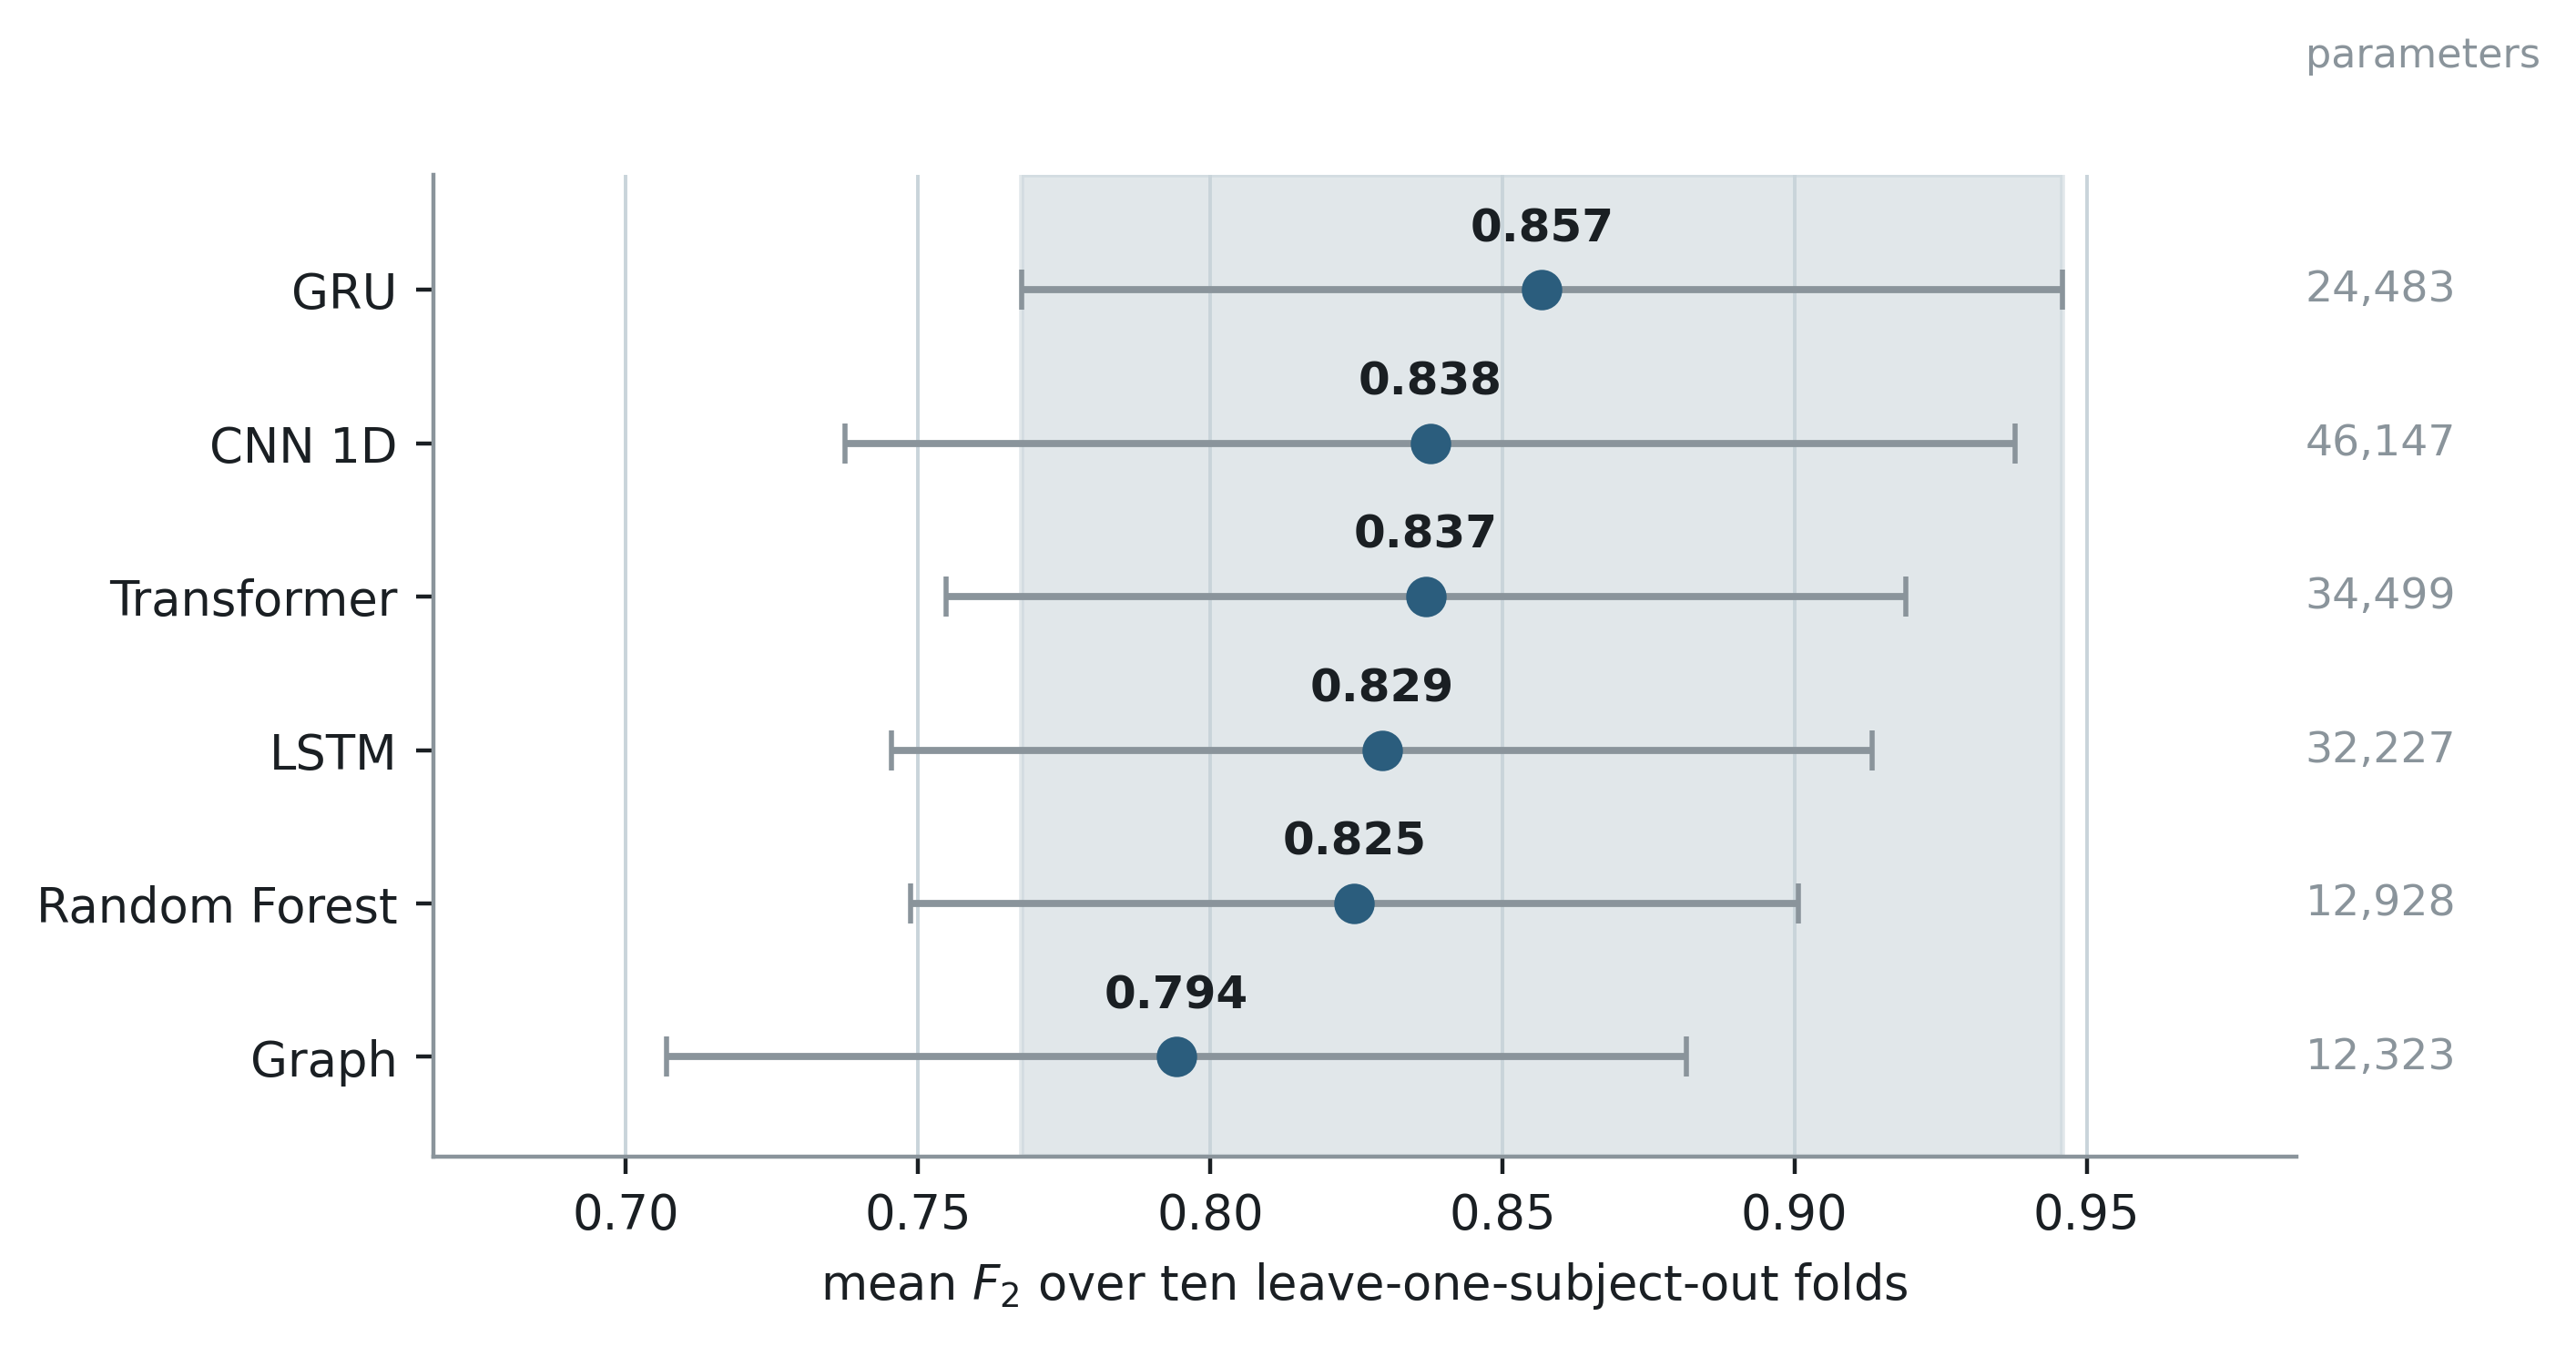
\includegraphics[width=\textwidth]{figure/fig_architetture_en.png}
\caption{Comparison between the six architectures. The error bars represent the dispersion across the ten subjects.}
\label{fig:architetture}
\end{figure}

\begin{figure}[htbp]
\centering
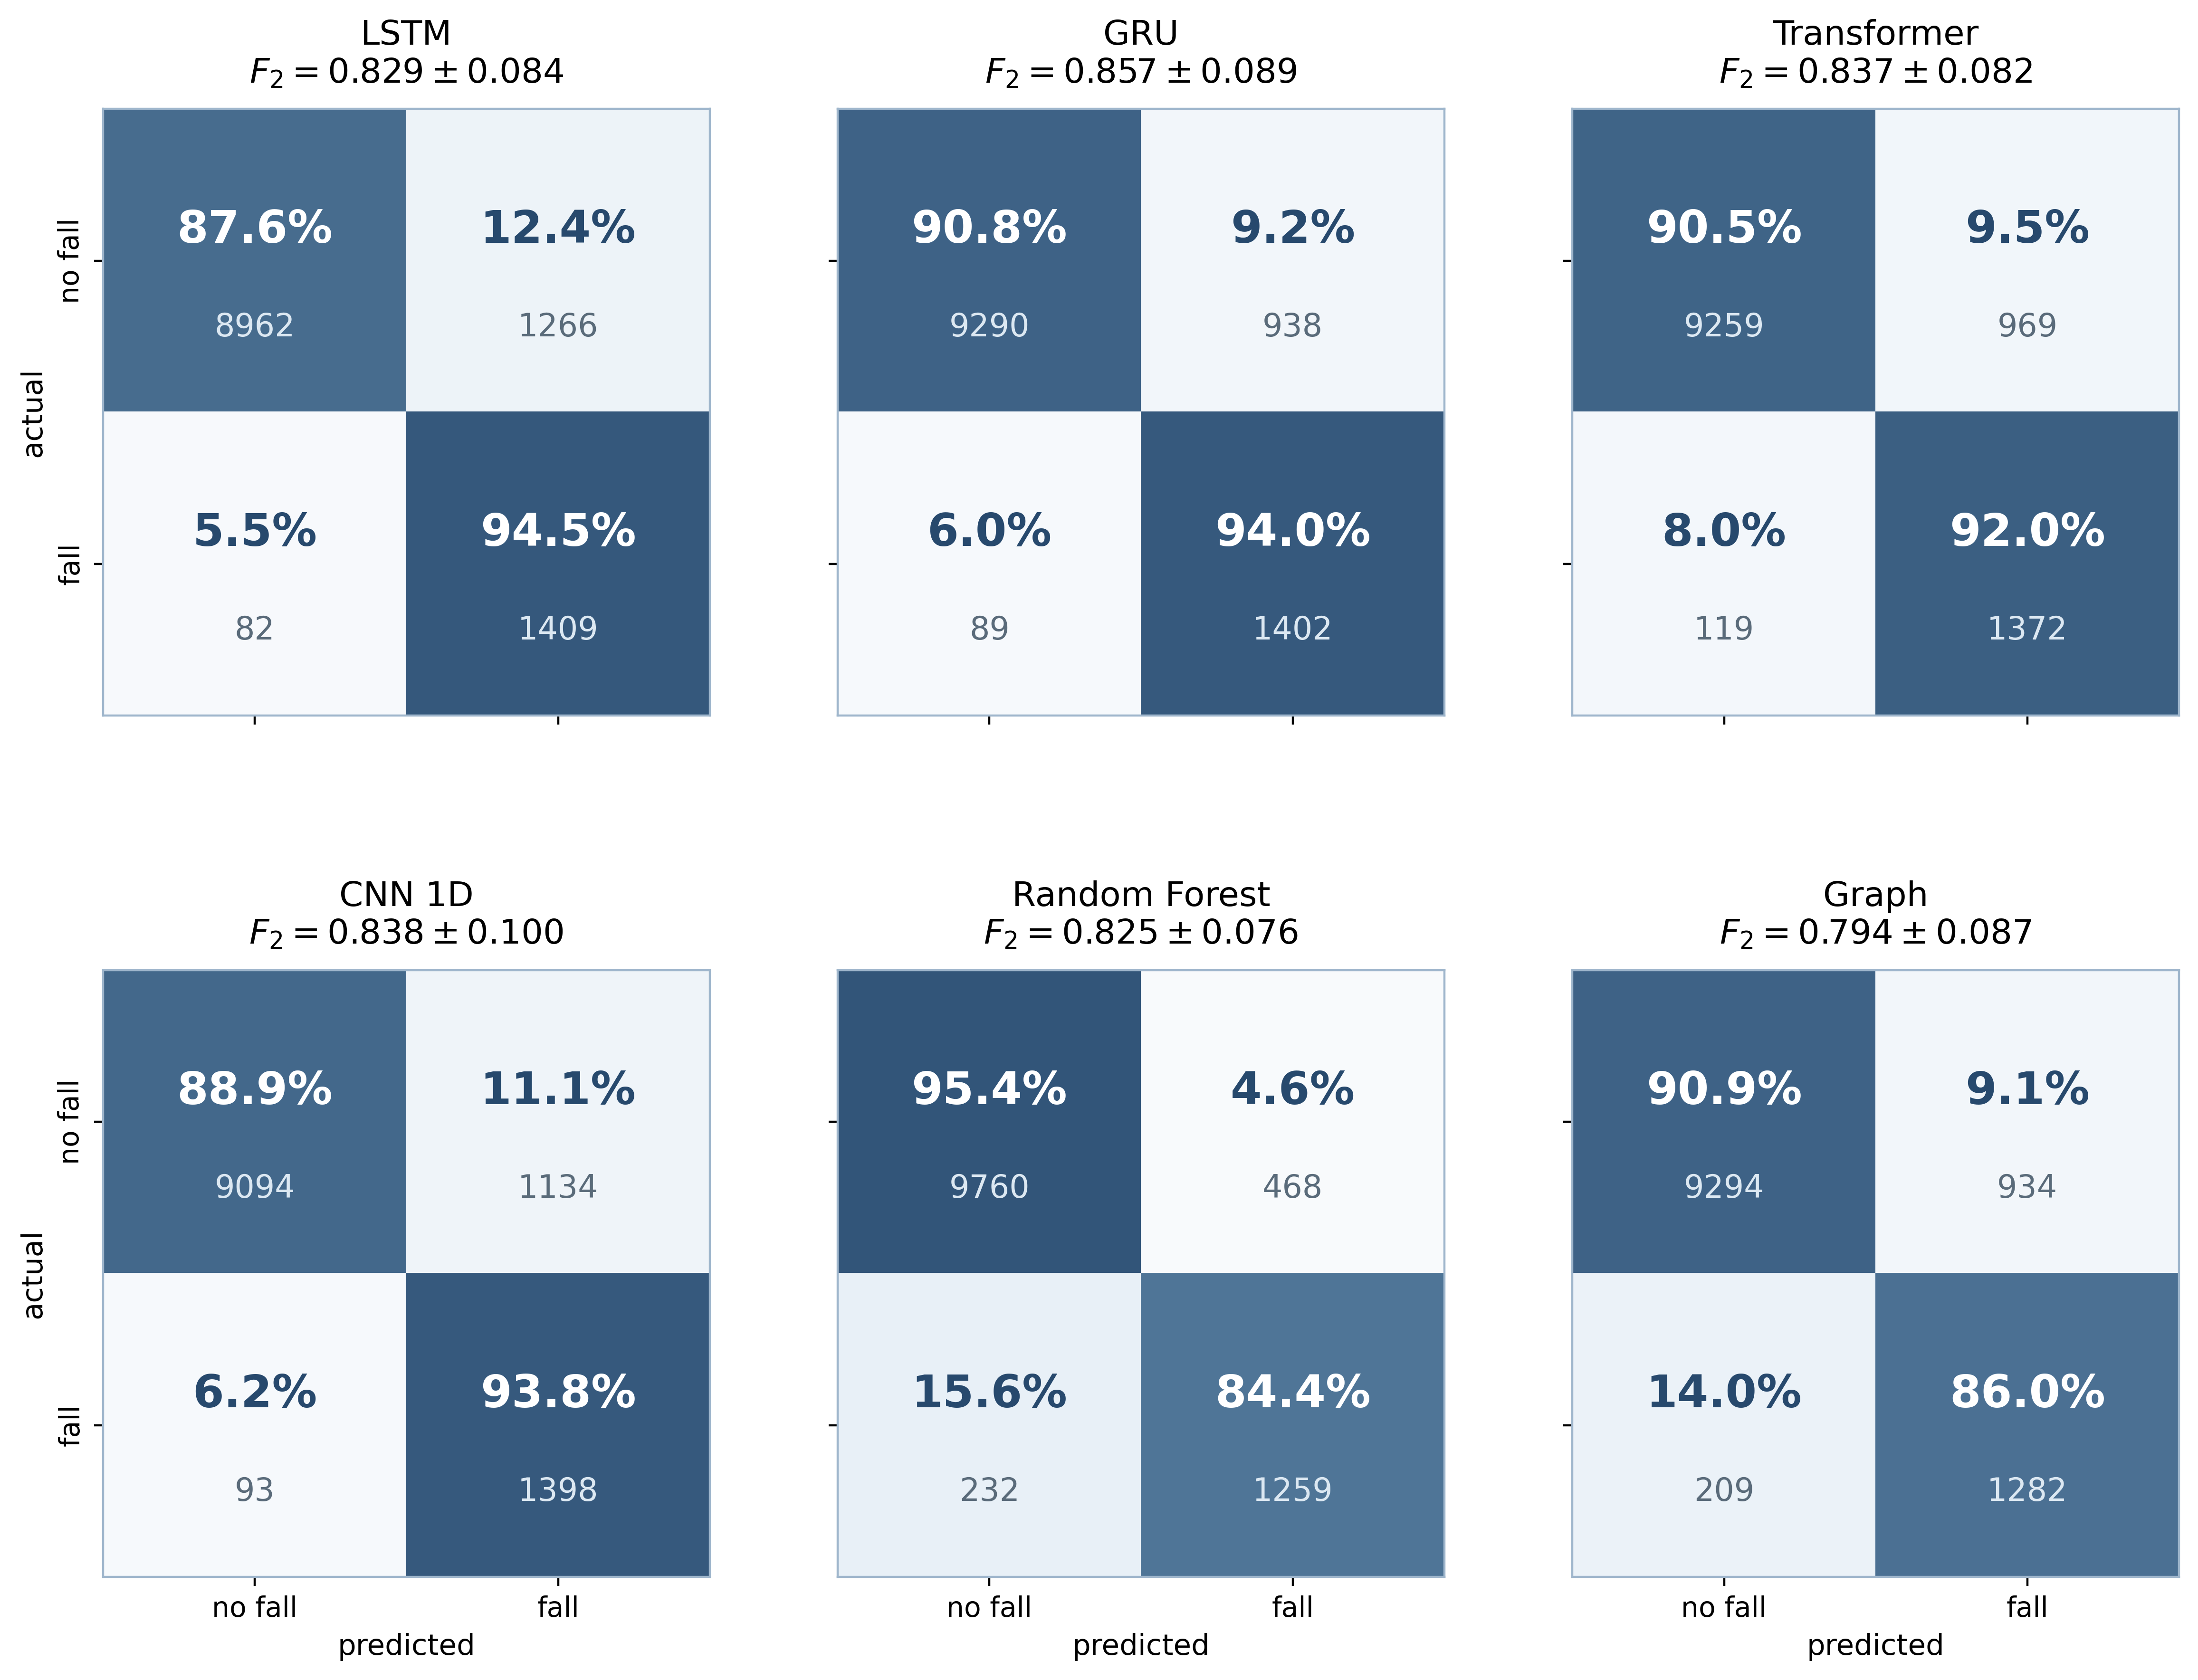
\includegraphics[width=0.85\textwidth]{figure/fig_confusione_en.png}
\caption{Confusion matrices of the six architectures, obtained by pooling the ten verification folds.}
\label{fig:confusione}
\end{figure}

The graph network reaches $F_2=0{,}794\pm0{,}087$. In this implementation the nodes represent the twelve features supplied to the classifier and not the body joints directly. The result therefore concerns this specific configuration and not graph networks applied to the skeleton in general.
The number of parameters shows no evident relationship with performance. The 1D CNN is the neural model with the largest number of parameters, but it does not reach the highest value of $F_2$. The GRU, by contrast, uses about 24\% fewer parameters than the LSTM while obtaining a higher $F_2$.

In order to check the differences on the individual subjects, the models were also compared fold by fold using the GRU as reference. The values obtained are $t=-1{,}16$ for the 1D CNN, $t=-1{,}22$ for the Transformer and $t=-1{,}24$ for the Random Forest. The LSTM and the graph network instead produce $t=-2{,}98$ and $t=-3{,}14$ respectively. Taking into account the five comparisons made against the GRU, however, the critical value corrected for multiple comparisons rises to about 3,25, and no difference exceeds it.

With the number of subjects available we therefore measure no clear difference between the main architectures considered. The architectures were not subjected to a systematic hyperparameter search. The comparison therefore concerns the configurations actually used, and not the respective families of models in general.

\subsection{Analysis of the differences and sample size}

The preceding configurations were evaluated on the same subjects. It is therefore possible to compare the results fold by fold and to use the variability observed in order to estimate how many subjects would be needed to detect the differences measured. Table~\ref{tab:numerosita} reports the mean difference, the value of the paired $t$ test and an estimate of the sample size required with $\alpha=0{,}05$ and 80\% power.

\begin{table}[htbp]
\centering
\caption{Sample size estimated in order to detect some of the differences observed.
The estimate uses a two-tailed paired $t$ test, with $\alpha=0{,}05$ and
80\% power.}
\label{tab:numerosita}
\begin{tabular}{lccc}
\toprule
\textbf{Comparison} &
\textbf{Difference} &
\textbf{$t$} &
\textbf{Subjects required} \\
\midrule
Window of 44 instead of 22 & $+0{,}091$ & $+3{,}62$ & 6 \\
GRU vs graph network & $-0{,}063$ & $-3{,}14$ & 8 \\
GRU vs LSTM & $-0{,}027$ & $-2{,}98$ & 9 \\
GRU vs Random Forest & $-0{,}032$ & $-1{,}24$ & 52 \\
GRU vs Transformer & $-0{,}020$ & $-1{,}22$ & 54 \\
GRU vs 1D CNN & $-0{,}019$ & $-1{,}16$ & 58 \\
DTW selection instead of all of A3 & $-0{,}007$ & $-0{,}21$ & 1.833 \\
Integral quantities added to A3 & $+0{,}001$ & $+0{,}18$ & 2.373 \\
\bottomrule
\end{tabular}
\end{table}

Between the GRU and the Random Forest the mean difference is 0,032, but it varies considerably across subjects and the estimated sample size rises to 52. Between the GRU and the LSTM the gap is slightly smaller, 0,027, but more consistent across the folds, and the estimate drops to nine subjects. The differences introduced by the DTW selection and by the integral quantities are instead very small with respect to the variability between subjects.

The length of the window and some definitions of the task, by contrast, produce more evident effects. Going from 22 to 44 samples increases the mean $F_2$ by 0,091, with $t=3{,}62$, and is therefore detectable even with the number of subjects available.

\section{Sensitivity analysis}
\label{sec:sensibilita}

Besides the main choices, some parameters of the pipeline were analysed while the rest of the configuration was kept unchanged: number of trees of the Random Forest, sampling frequency, window length, availability of the landmarks and noise in the coordinates. The aim is not to find the optimal value of every parameter, but to verify how far performance depends on the choices adopted.

\subsection{Model size}
\label{sec:dimensione}

The first analysis concerns the number of trees of the Random Forest. The configuration used in the pipeline employs 50 trees, a value inherited from the initial prototype and not chosen through an experimental search. Six configurations between 10 and 400 trees were therefore compared, keeping data, features and evaluation protocol unchanged.

\begin{figure}[ht]
    \centering
    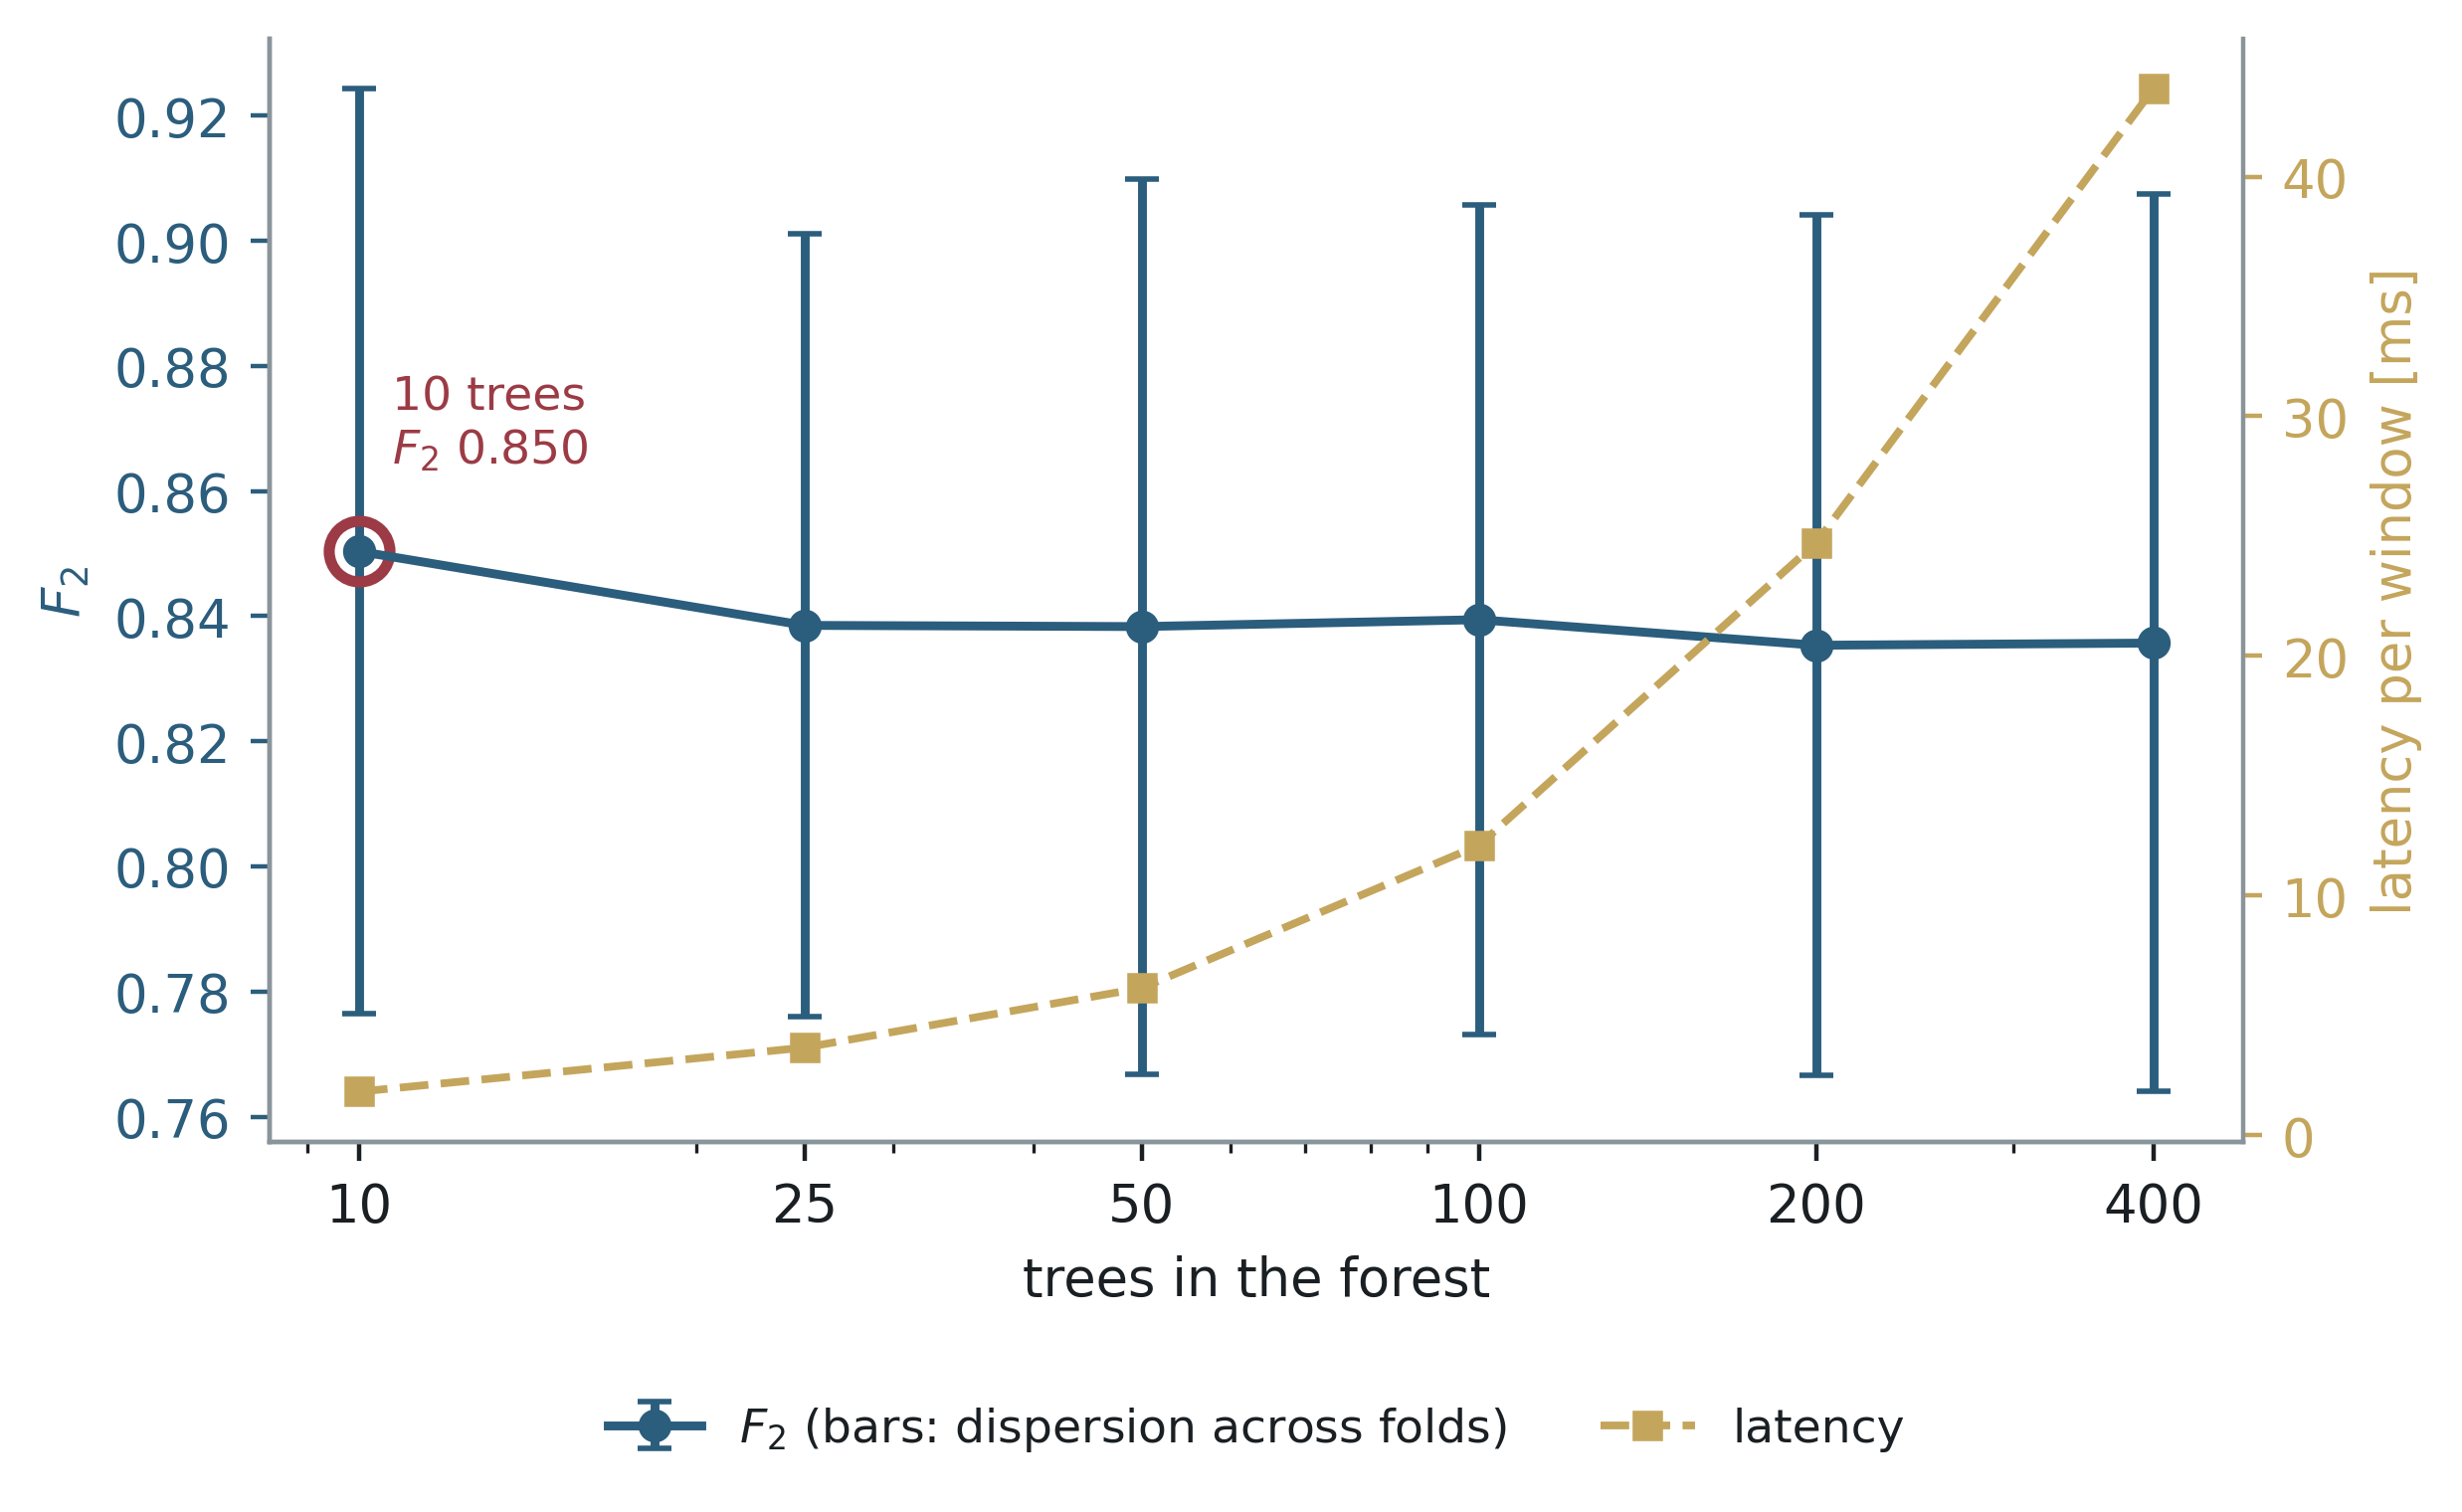
\includegraphics[width=\textwidth]{figure/fig_dimensione_en.png}
    \caption{Performance and latency as the number of trees of the
    Random Forest varies, over the 10 LOSO folds. The error bars represent the dispersion across subjects.}
    \label{fig:dimensione}
\end{figure}

With 10 trees $F_2=0{,}850\pm0{,}074$ is obtained, with 50 trees $0{,}838\pm0{,}072$ and with 400 trees $0{,}836\pm0{,}072$. The whole variation is about 0,015, against a dispersion across subjects of about 0,07. The computational cost, by contrast, changes markedly: the time per window goes from about 1,8~ms with 10 trees to 43,7~ms with 400, while the number of nodes grows from 1.881 to 76.065.

The highest mean value of $F_2$ is obtained with 10 trees, but the difference with respect to the other configurations is very small compared with the variability between subjects, and the corresponding dispersion bars overlap widely.
The trials therefore show no improvement in performance from increasing the size of the forest. We keep 50 trees, that is the configuration already in use, without regarding it as an optimal value.

\subsection{Effect of the frame rate}
\label{sec:framerate}

Another parameter analysed is the frequency at which the samples are
supplied to the classifier. UP-Fall is acquired at about 18~fps, whereas the
configuration intended for the device uses about 9 samples per second.
The effect of halving the frequency was therefore verified. This trial belongs to the preliminary five-subject configuration and is the only sensitivity analysis in the section that was not subsequently repeated on the ten subjects.

\begin{table}[ht]
\centering
\caption{Effect of halving the frame rate in the 5-subject configuration.}
\label{tab:framerate}
\begin{tabular}{lcc}
\toprule
 & \textbf{18 fps} & \textbf{9 fps} \\
\midrule
Missed falls & 6,8\% & 12,4\% \\
Variation of $F_2$ & -- & $-0{,}045$ \\
\bottomrule
\end{tabular}
\end{table}

Halving the frequency, missed falls go from 6,8\% to 12,4\%, while $F_2$ decreases by about 0,045. The loss therefore concerns recall above all. The variation of $F_2$ is smaller because the reduction in recall is partly offset by precision. Here too the overall metric alone cannot describe the behaviour of the classifier fully.

The effect of the time interval used in computing the derivatives was moreover verified. The final pipeline uses the $\Delta t$ derived from the actual timestamps instead of the nominal frequency. With respect to the computation based on a fixed 18~fps, the mean difference of $F_2$ over the ten subjects is $-0{,}006$, with $t=-1{,}15$.

The effect is therefore small. This is consistent with the features selected: of the twelve features used, eight are integral, two static and only two are derivatives and depend directly on the value of $\Delta t$. The frequency of 9~fps is kept as the reference for execution on the board, where the frequencies actually obtained are analysed in Chapter~\ref{cap:edge}.

\subsection{Length of the temporal window}
\label{sec:lunghezza_finestra}

The configuration adopted uses windows of $L=22$ samples, about 2,44~s at 9~fps. The median duration of the fall transition is, however, about 3,11~s. It was therefore verified whether a longer window might contain the whole movement better. Four lengths were compared: 22, 28, 36 and 44 samples.

\begin{figure}[htbp]
\centering 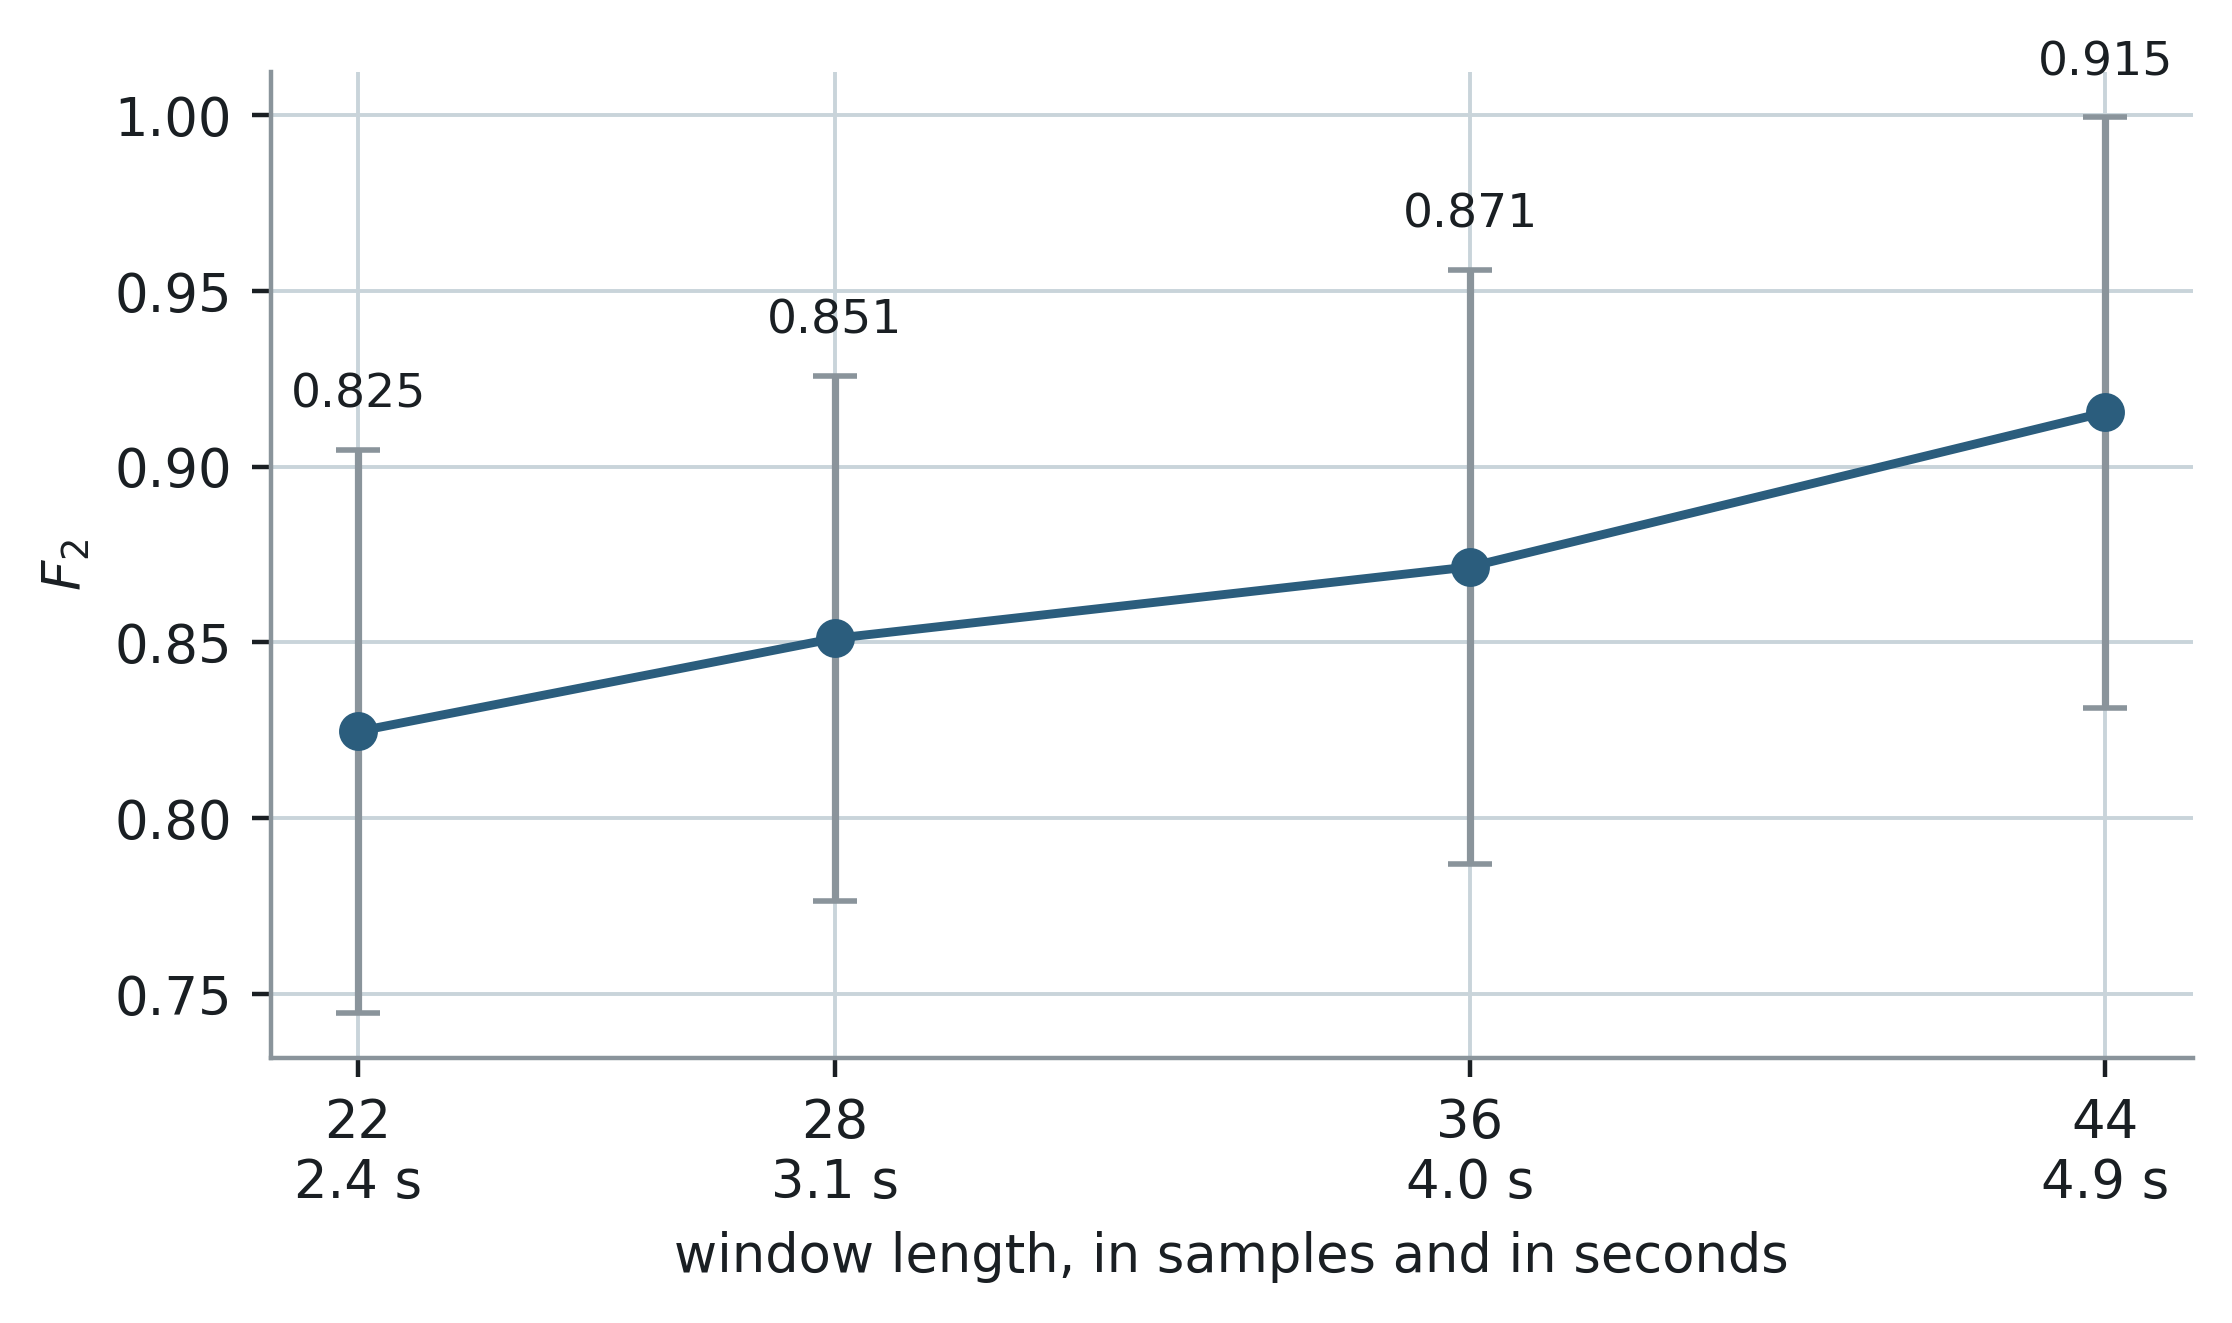
\includegraphics[width=\textwidth]{figure/fig_finestra_en.png}
\caption{Mean value of $F_2$ as the length of the window varies, over the ten LOSO folds.}
\label{fig:finestra}
\end{figure}

\begin{table}[htbp]
\centering
\caption{Performance as the length of the temporal window varies.}
\label{tab:finestra}
\begin{tabular}{ccccc}
\toprule
\textbf{$L$} & \textbf{Duration} & \textbf{$F_2$} & \textbf{Recall} & \textbf{FN / FP} \\
\midrule 22 & 2,4 s & $0{,}825 \pm 0{,}080$ & 0,849 & 232 / 468 \\
28 & 3,1 s & $0{,}851 \pm 0{,}075$ & 0,880 & 164 / 414 \\
36 & 4,0 s & $0{,}871 \pm 0{,}085$ & 0,900 & 113 / 341 \\
44 & 4,9 s & $0{,}915 \pm 0{,}084$ & 0,945 & \phantom{0}53 / 249 \\
\bottomrule
\end{tabular}
\end{table}

Performance increases steadily with the length. Going from 22 to 44 samples, $F_2$ rises from 0,825 to 0,915 and recall from 0,849 to 0,945.
False negatives and false positives decrease at the same time, from 232 to 53 and from 468 to 249 respectively. The improvement is therefore not due solely to a shift in the trade-off between precision and recall.

The paired comparison between 22 and 44 samples produces a mean difference of $+0{,}091$ of $F_2$, with $t=3{,}62$.
Despite this result, $L=22$ is retained in the final configuration. A window of 44 samples requires about 4,9~s before a decision can be produced, against 2,44~s with 22 samples.
The choice is therefore a compromise between performance on the benchmark and the time needed to collect the sequence. The contribution of the window to the overall latency is measured in Chapter~\ref{cap:edge}.

\subsection{Sensitivity to the loss of landmarks}
\label{sec:occlusioni}

The availability of the landmarks may be reduced when some parts of the body are not detected by the pose estimator. In order to verify how far this can affect classification, a controlled simulation was carried out in which certain points of the body were made unavailable.

 The landmark treated as unavailable is held at the last value observed instead of being set to zero, thereby avoiding an artificial displacement towards the origin of the image. Both anatomical groups and random groups of increasing size were tried. The configuration without occlusions has $F_2=0{,}853\pm0{,}071$.

\begin{table}[htbp]
\centering
\caption{Variation of $F_2$ obtained by freezing different groups of landmarks.}
\label{tab:occlusioni}
\begin{tabular}{lcc}
\toprule
\textbf{Group} & \textbf{Points} & \textbf{$\Delta F_2$} \\
\midrule
Shoulders & 2 & $-0{,}037$ \\
Ankles & 2 & $-0{,}012$ \\
Left half & 6 & $-0{,}004$ \\
Nose & 1 & $-0{,}002$ \\
Knees + ankles & 4 & $+0{,}001$ \\
Hips & 2 & $+0{,}015$ \\
\midrule
Random 11\% & 1 & $-0{,}002$ \\
Random 22\% & 2 & $+0{,}001$ \\
Random 33\% & 3 & $+0{,}003$ \\
Random 55\% & 5 & $-0{,}032$ \\
\bottomrule
\end{tabular}
\end{table}

\begin{figure}[htbp]
\centering
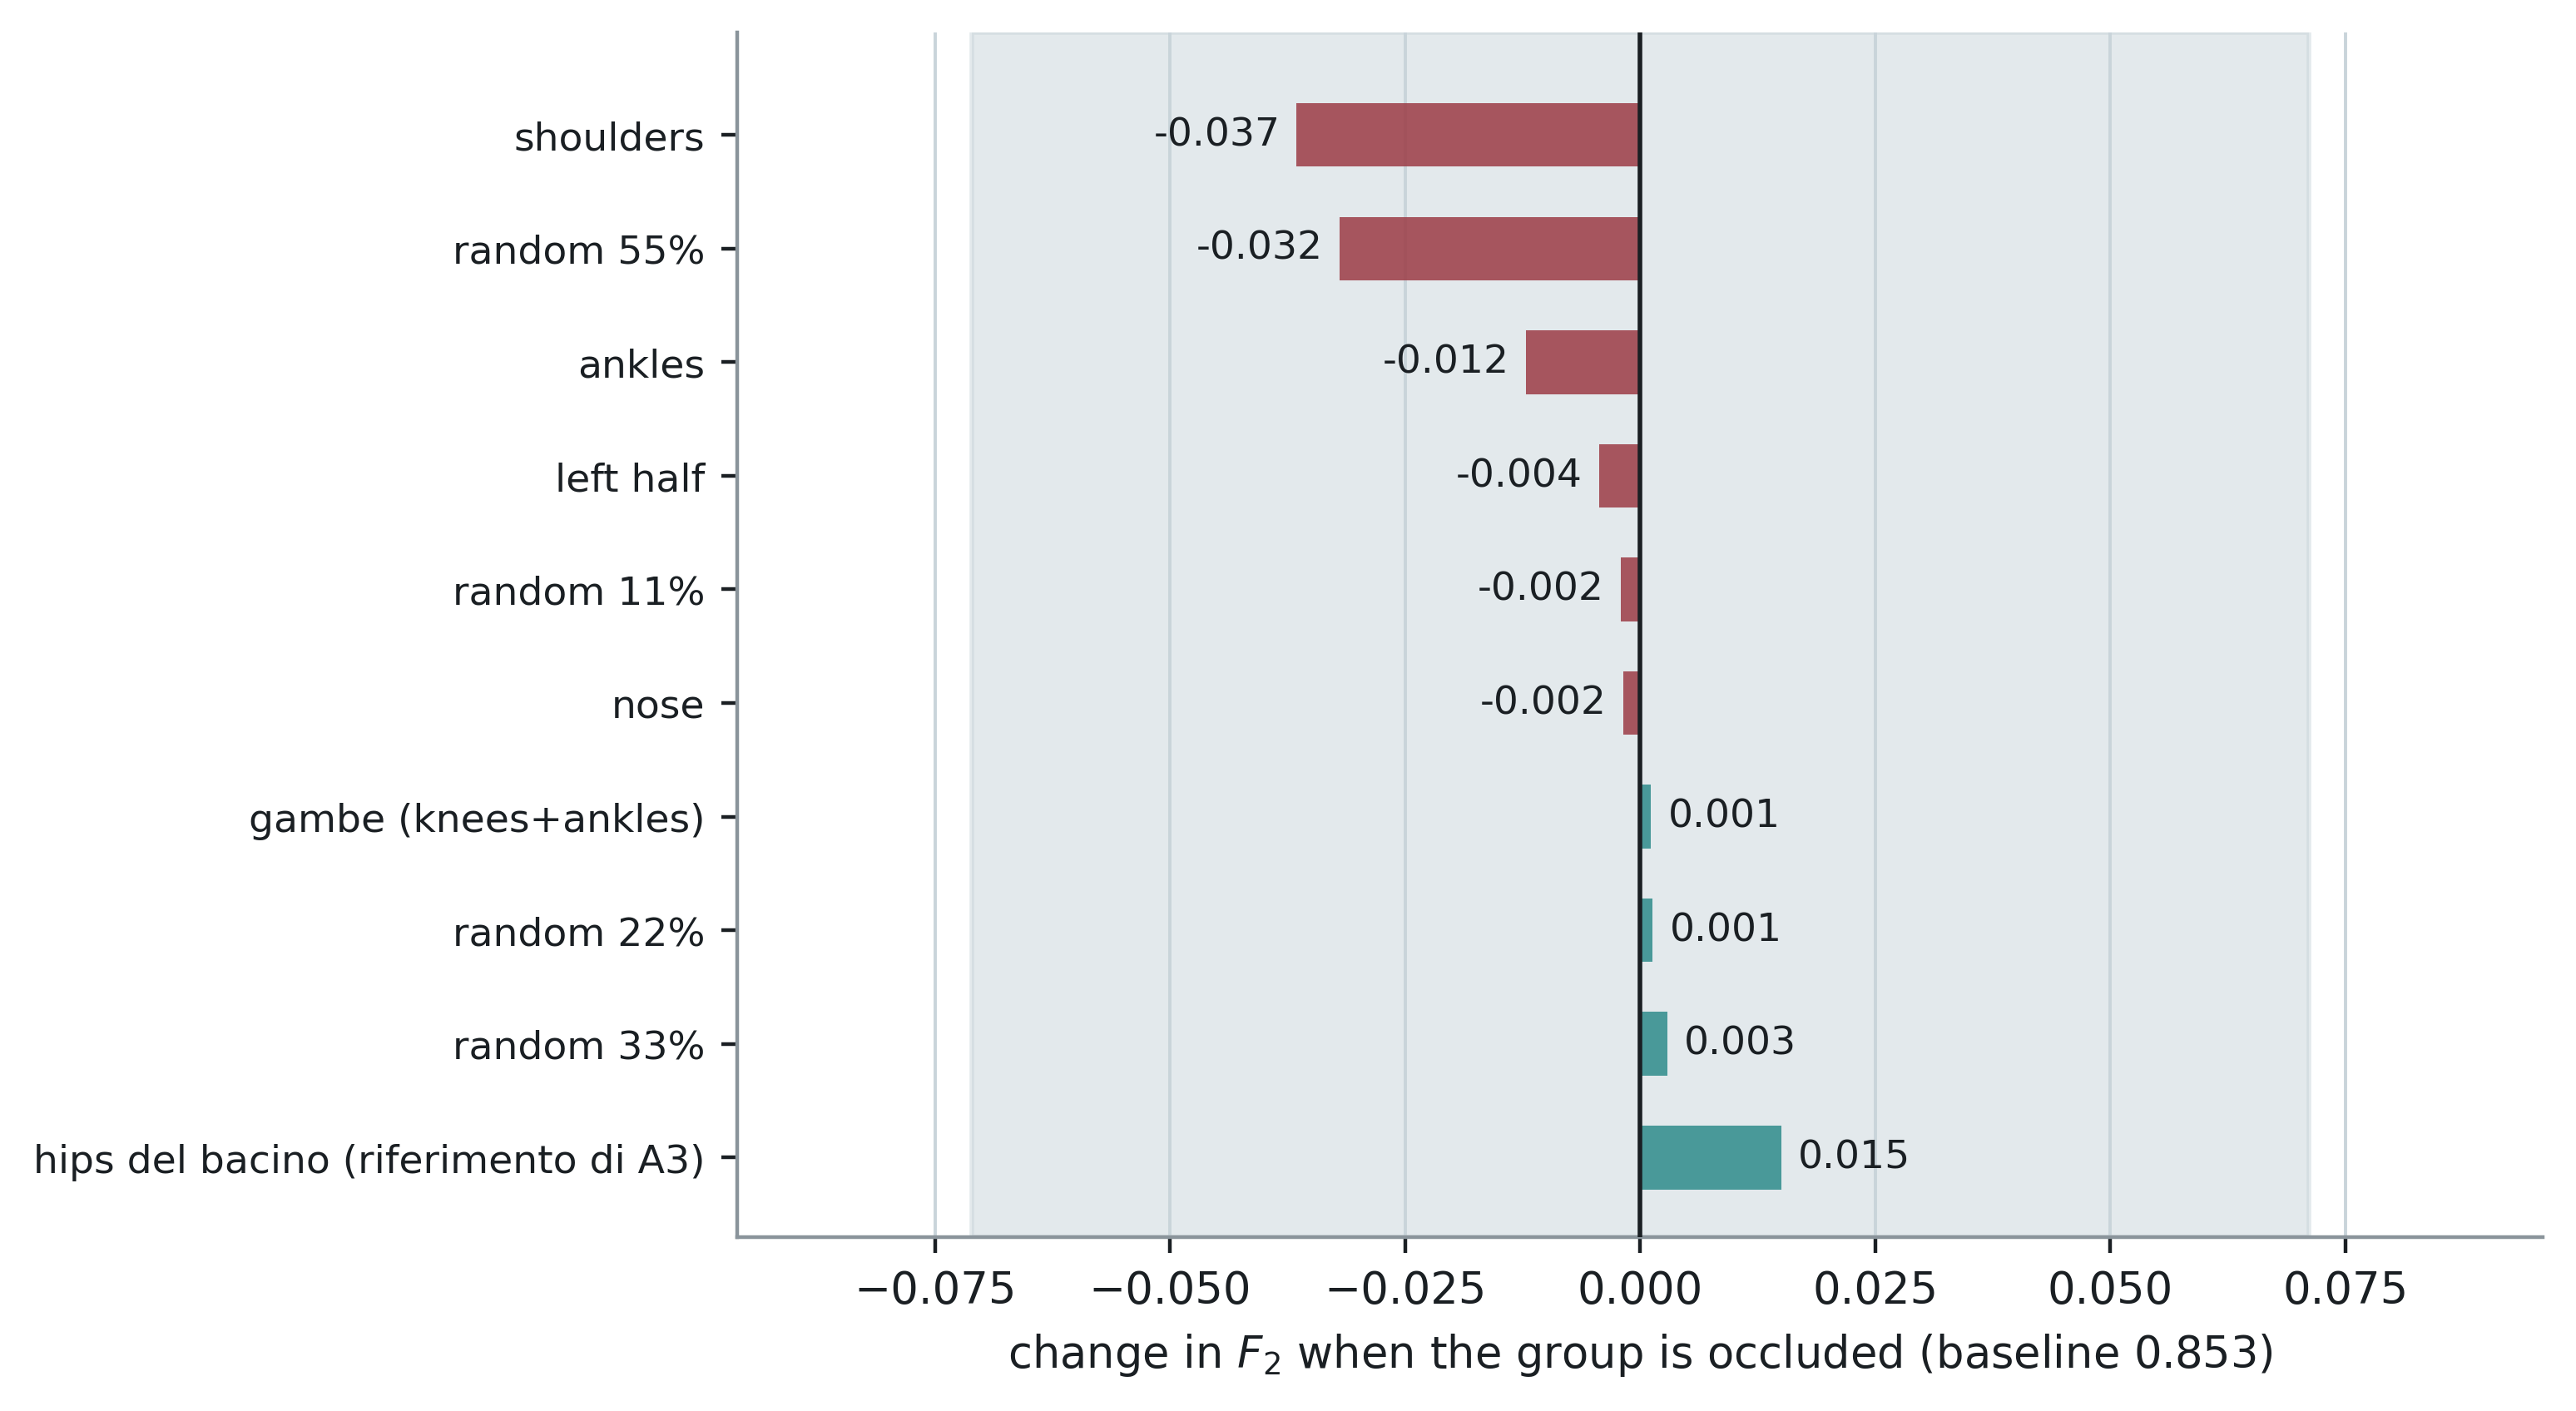
\includegraphics[width=0.86\textwidth]{figure/fig_occlusioni_en.png}
\caption{Effect of the simulated occlusions on the different groups of landmarks.}
\label{fig:occlusioni}
\end{figure}

The largest degradation is 0,037 of $F_2$ and is obtained by masking the shoulders. This value is about half the dispersion across subjects, 0,071. None of the groups considered therefore causes, on its own, a variation larger than the variability already present between people.
The small positive variations are not interpreted as improvements, but as experimental fluctuations.

Among the anatomical groups, the largest variation is observed by masking the shoulders.
Repeating the same trial with the previous subset of features, however, the loss goes from $-0{,}037$ to $-0{,}019$. Sensitivity therefore also depends on the features built from the landmarks.
A particular case concerns the hips. When their position is not updated, some features of representation A3 remain indirectly referred to a more stable position in the image plane. With a fixed camera this may reintroduce part of the information about the position of the person in the scene.

The experiment had not, however, been designed to assess the feature $h_{\text{pav}}$ directly, and cannot therefore be regarded as a verification of its effectiveness. The trial concerns simulated occlusions in any case, and does not warrant the conclusion that the system is robust to extensive real occlusions.

\subsection{Temporal regularity of the quantities}
\label{sec:autocorrelazione}

In order to compare the temporal regularity of the dynamic quantities, the one-step autocorrelation was measured:

\[
\rho_1 =
\frac{\operatorname{Cov}(x_t,x_{t-1})}
{\sigma_{x_t}\sigma_{x_{t-1}}}.
\]

The computation was carried out only within continuous stretches with a valid pose. The results are reported in Table~\ref{tab:autocorrelazione}.

\begin{table}[htbp]
\centering
\caption{One-step autocorrelation of the main dynamic quantities}
\label{tab:autocorrelazione}
\begin{tabular}{lc}
\toprule
\textbf{Quantity} & $\boldsymbol{\rho_1}$ \\
\midrule
\multicolumn{2}{l}{\emph{Instantaneous derivatives}} \\
\quad Variation of the trunk angle & 0,221 \\
\quad Angular velocity of the trunk & 0,494 \\
\quad Velocity of the hips & 0,499 \\
\quad Velocity of the head & 0,535 \\
\midrule
\multicolumn{2}{l}{\emph{Integral quantities}} \\
\quad Descent of the hips & 0,818 \\
\quad Path of the hips & 0,882 \\
\quad Excursion of the trunk & 0,988 \\
\bottomrule
\end{tabular}
\end{table}

The derivatives have values between 0,221 and 0,535, while the integral quantities range between 0,818 and 0,988. Even the lowest value of the integral quantities remains above the highest value of the derivatives, and they are therefore more regular over time. This comparison describes, however, only the continuity of the signals, and does not show that a feature with a higher autocorrelation is also more useful for classification.

\subsection{Sensitivity to landmark noise}
\label{sec:rumore}

Finally, the sensitivity to noise in the coordinates of the landmarks was verified.
Errors in pose estimation were simulated by adding independent Gaussian noise. The standard deviation $\sigma$ is expressed as a fraction of the length of the torso, so as not to depend on the apparent size of the person in the image.

Three configurations were compared: the representation without the integral quantities (A3base), the complete one (A3) and the subset selected by DTW (DTW). The results are reported in Table~\ref{tab:rumore} and in Figure~\ref{fig:rumore}.

\begin{table}[htbp]
\centering
\caption{Value of \(F2\) as the Gaussian noise added to the landmarks increases.}
\label{tab:rumore}
\begin{tabular}{lccc}
\hline
$\boldsymbol{\sigma}$ & \textbf{without integrals (10)} & \textbf{with integrals (13)} & \textbf{selected subset (12)}\\
\hline
0     & 0,874 & 0,858 & 0,857 \\
0,005 & 0,863 \,(--0,011) & 0,864 \,(+0,006) & 0,844 \,(--0,012) \\
0,010 & 0,855 \,(--0,018) & 0,866 \,(+0,008) & 0,863 \,(+0,007) \\
0,020 & 0,864 \,(--0,010) & 0,846 \,(--0,012) & 0,836 \,(--0,021) \\
0,040 & 0,863 \,(--0,011) & 0,856 \,(--0,002) & 0,825 \,(--0,031) \\
\hline
\end{tabular}
\end{table}

\begin{figure}[htbp]
\centering
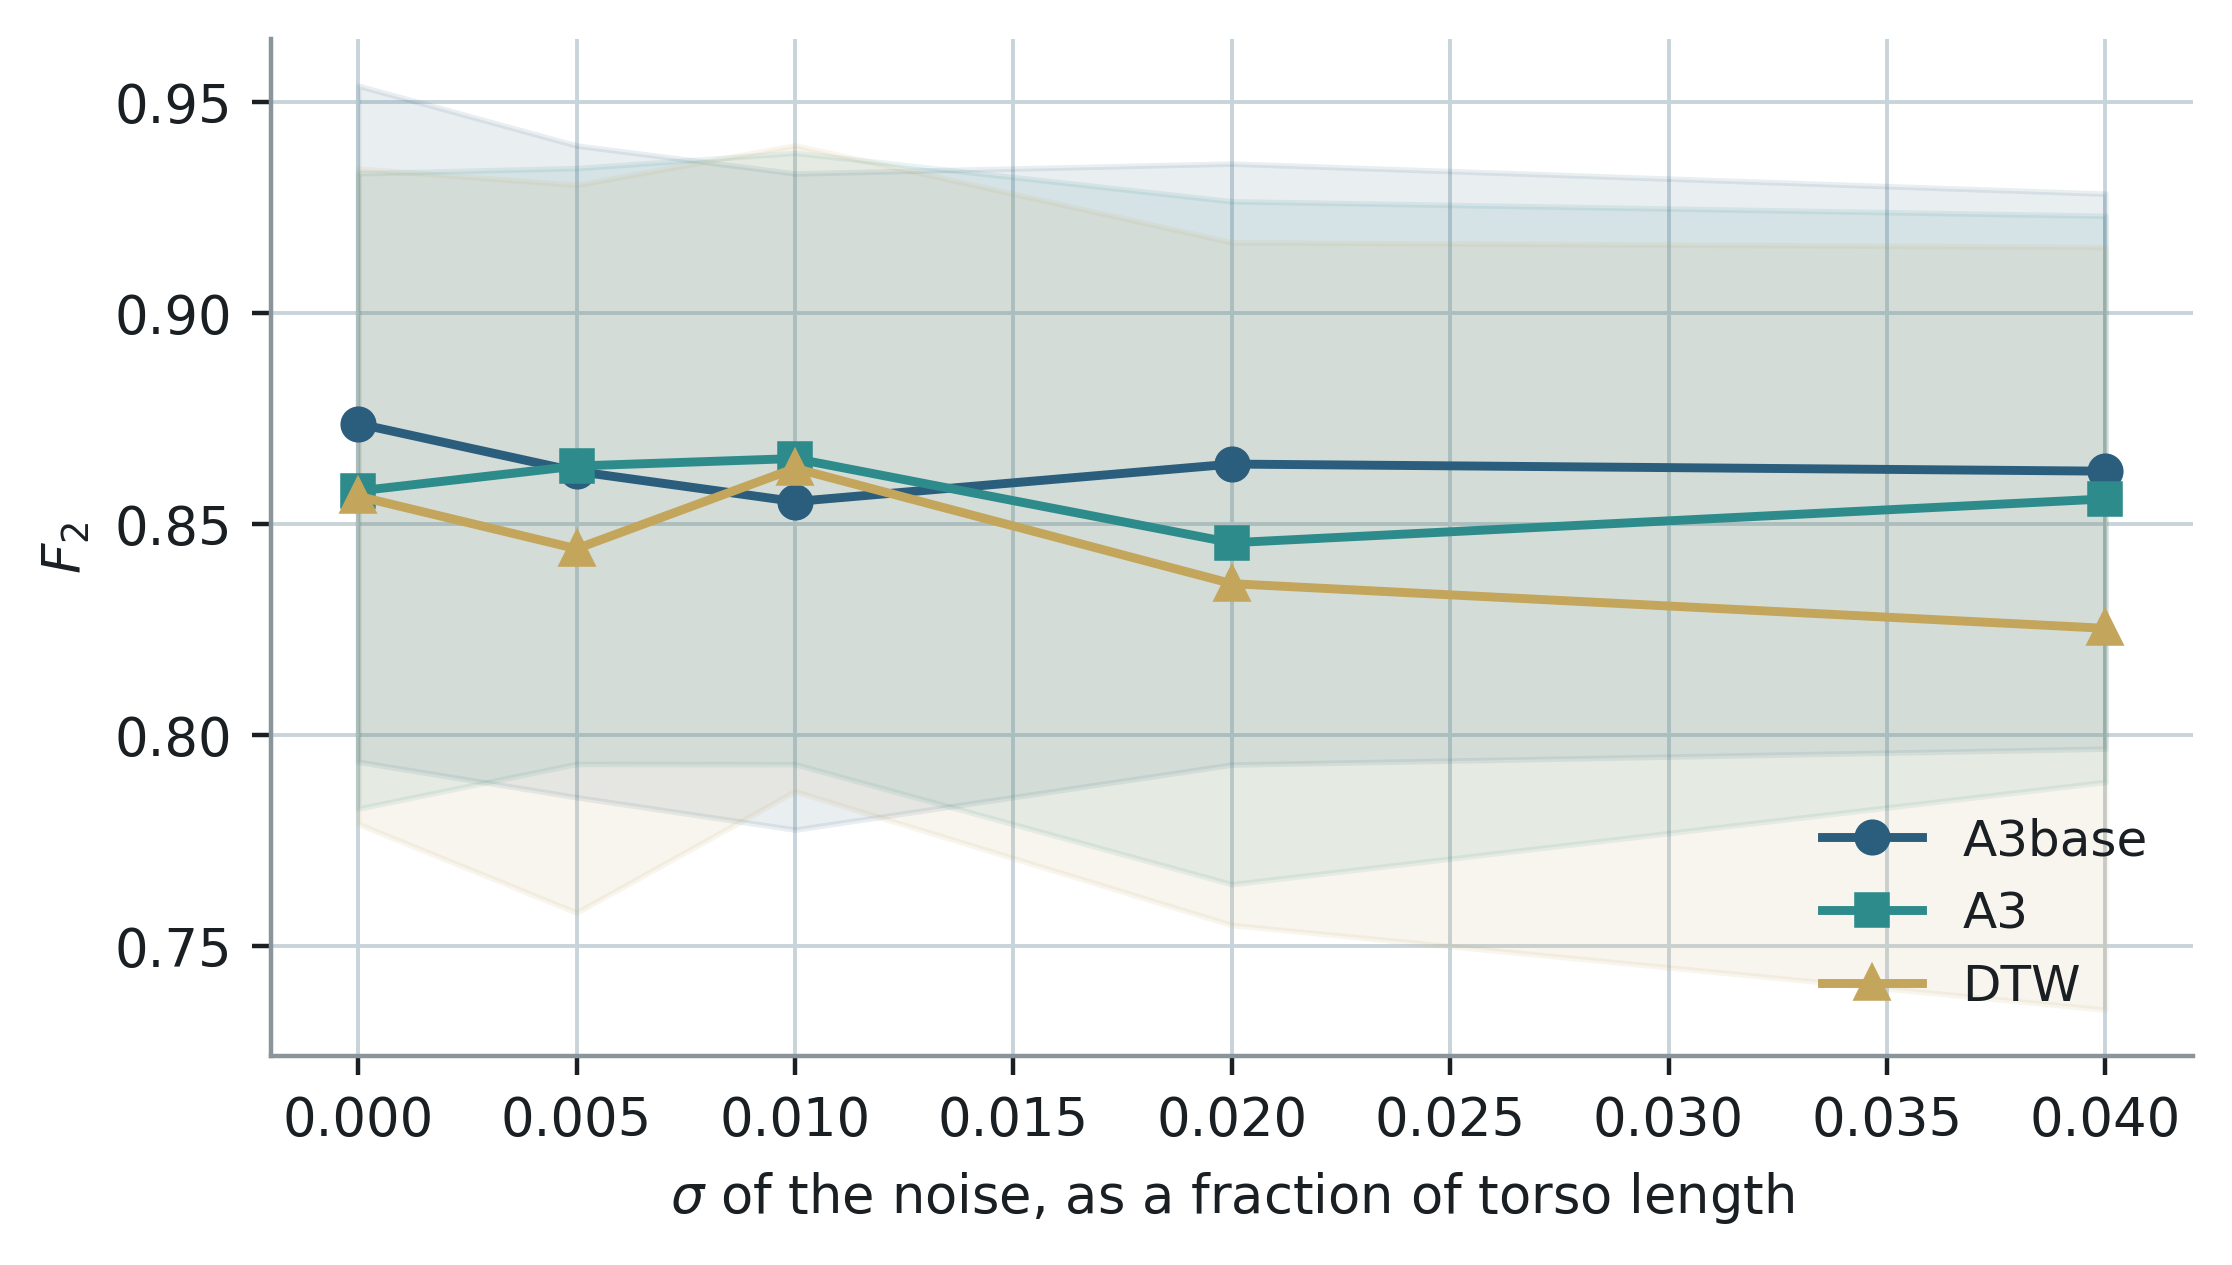
\includegraphics[width=0.86\textwidth]{figure/fig_rumore_en.png}
\caption{Performance as the Gaussian noise added to the coordinates of the landmarks increases, for the three feature sets considered.}
\label{fig:rumore}
\end{figure}

Even with \(\sigma=0{,}04\), the largest degradation is 0,031 of $F_2$, therefore below the dispersion across subjects, which is about 0,08.
Nor do the integral quantities show a greater degradation than the instantaneous quantities alone: between the representation without integral quantities and the complete one, that is at parity of everything except the three integral quantities, the degradation at $\sigma=0{,}04$ is $0{,}011$ and $0{,}002$ respectively. The positive variations observed at intermediate noise levels are fluctuations within the dispersion between subjects, and are not interpreted as improvements.

This result does not mean that the integral quantities eliminate the noise. Path, excursion and descent still depend on the coordinates of the landmarks and may therefore vary when these are perturbed. Under the conditions considered, however, independent Gaussian noise has a limited effect on the final performance. In the domestic recordings a different error was instead observed. In some cases the estimator switches from one plausible configuration of the pose to another, and the new configuration remains coherent for several frames. This behaviour can be interpreted by the temporal features as real movement. One example was observed on the excursion of the trunk, as reported in Table~\ref{tab:ambiguita}.

\begin{table}[htbp]
\centering
\caption{Excursion of the trunk over a sliding window in two domestic recordings.}
\label{tab:ambiguita}
\begin{tabular}{lcc}
\hline
 & \textbf{Median} & \textbf{Maximum} \\
\hline
Person still on a sofa & 9,0$^\circ$ & 93,5$^\circ$ \\
Fall & 9,0$^\circ$ & 60,7$^\circ$ \\
\hline
\end{tabular}
\end{table}

In this case a person who is still produces a maximum excursion greater than that of the fall. The increase does not correspond to real movement of the body, but to the estimator switching between two different poses. Gaussian noise therefore does not reproduce all the errors that may appear during real operation. If a wrong pose remains stable for several frames it can be interpreted as real movement by the integral quantities too, and even a temporal filter may not be enough to correct it.

\section{Effect of the definition of the task}
\label{sec:compito-risultati}

So far the definition of the positive class has been kept unchanged. In this analysis the task assigned to the classifier is instead modified, distinguishing the fall transition from the subsequent state in which the person remains on the ground. Three tasks were considered:
\begin{enumerate}
\item \emph{event}: only the fall transition is positive;
\item \emph{state}: only the post-fall state is positive;
\item \emph{alarm}: transition and post-fall state are both considered positive.
\end{enumerate}

Model, features and protocol are kept unchanged. What changes is the prevalence of the positive class in the training set, because the three formulations use different portions of the fall episode. In order to make the results comparable, all the models are evaluated on the same alarm label, which treats both the transition and the post-fall state as positive.

Greater attention was paid in the analysis to the windows in which the person lies down voluntarily, because they are hard cases to distinguish from the post-fall state, the final configuration of the body being very similar to that of a person who has remained on the ground after a fall. Precisely in order to isolate them, the three tasks are defined on the OmniFall annotations introduced in
Section~\ref{sec:compito}, and not on the hand-made labels: the latter assign the normal class to every frame of the daily-activity recordings, and therefore cannot separate voluntary lying down from the rest. The classes \texttt{fall} and \texttt{fallen} do make it possible, and a window turns out positive when it contains at least five of their frames.

The resulting set does not coincide with the one used in the comparisons between
architectures and representations: it comprises 12.140 windows, of which
1.399 are positive, that is $11{,}5\%$, against the 11.719 windows and
1.491 positives ($12{,}72\%$) of Section~\ref{sec:metriche}. The same
definition of the positive is adopted in the sensitivity analyses of
Sections~\ref{sec:occlusioni} and~\ref{sec:rumore}, and is the reason why the
reference values reported there do not coincide with those of
Table~\ref{tab:architetture}.

\begin{table}[htbp]
\centering
\caption{Performance obtained with the three definitions of the task, keeping model, features and protocol unchanged.}
\label{tab:compiti}
\small
\begin{tabularx}{\textwidth}{@{}l c c c c >{\centering\arraybackslash}X@{}}
\toprule
\textbf{Task} &
\textbf{Train. prev.} &
\textbf{$F_2$} &
\textbf{Recall} &
\textbf{Precision} &
\textbf{Hard negatives} \\
\midrule
Event  & 0,047 & $0{,}415 \pm 0{,}083$ & 0,364 & 0,990 & \phantom{0}0,04\% \\
State   & 0,089 & $0{,}587 \pm 0{,}094$ & 0,552 & 0,874 & \phantom{0}8,4\% \\
Alarm & 0,115 & $0{,}830 \pm 0{,}066$ & 0,836 & 0,841 & 11,7\% \\
\bottomrule
\end{tabularx}
\end{table}

\begin{figure}[ht]
\centering
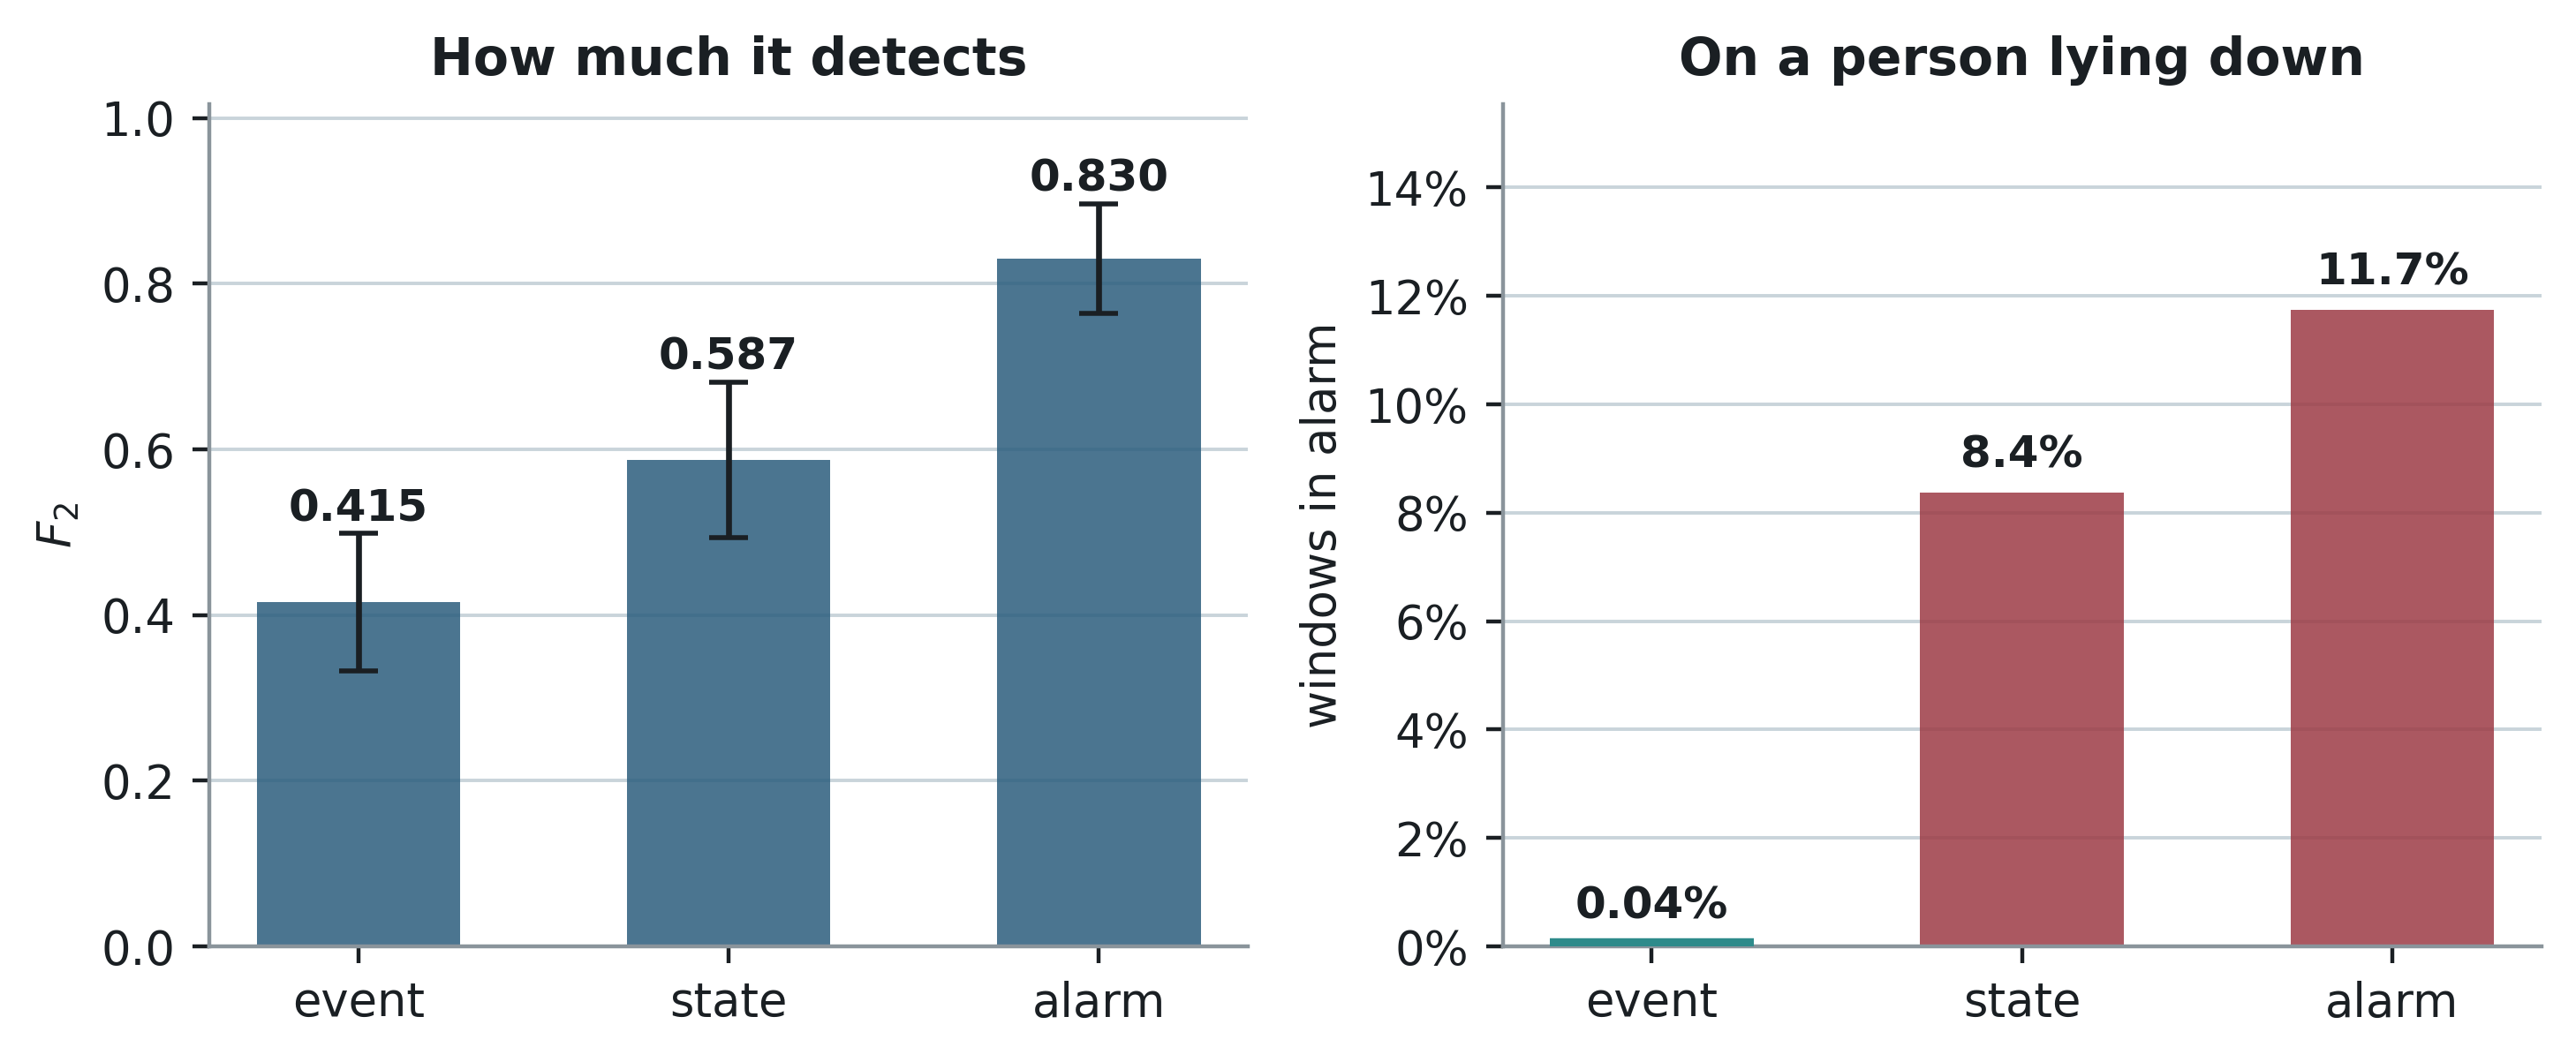
\includegraphics[width=\textwidth]{figure/fig_compiti_en.png}
\caption{Comparison between the three definitions of the task. On the left
$F_2$ is reported; on the right the share of windows flagged as positive
during the act of lying down voluntarily.}
\label{fig:compiti}
\end{figure}

The \emph{alarm} formulation reaches the highest mean value of $F_2$, 0,830, and the highest recall, 0,836. The \emph{state} task reaches 0,587, while the \emph{event} task stops at 0,415.

The difference concerns recall above all. The model trained on the transition alone recognises less often the windows in which the person is already on the ground, which are nonetheless treated as positive in the common evaluation. Precision instead shows the opposite behaviour. The event task reaches 0,990 and classifies as positive only one of the 2.234 windows relating to lying down voluntarily. The share rises to 8,4\% for the state task and to 11,7\% for the alarm task.

The three formulations therefore produce a different trade-off between recall and false positives. The \emph{event} task is more selective, but loses part of the positive windows. The \emph{alarm} task increases recall and $F_2$, but introduces more errors in the activities that end in a posture similar to the post-fall state. The definition of the task therefore has a considerable effect on the results, greater than the one observed by changing the architecture of the classifier alone. The operational behaviour of the three formulations is taken up again in Chapter~\ref{cap:edge}, where the comparison is made at the level of events and of false alarms per hour.

\subsection{Dynamics of the fall and voluntary lying down}

A fall and the voluntary act of lying down may bring the person into a similar final position, but they differ in the movement that precedes it.
In the definition of the task it is possible to treat as the positive class the \emph{event}, that is the phase in which the fall occurs, the subsequent \emph{state}, when the person is already on the ground, or both conditions for the purposes of the alarm.

This distinction matters because the final configuration of the body may be similar in the two cases, whereas the dynamics by which it is reached may be very different. In order to verify this difference, some dynamic quantities were compared during the transition and during the subsequent state on the ground. The ratios between the medians are reported in Table~\ref{tab:dinamica}.

\begin{table}[htbp]
\centering
\caption{Ratio between the medians of the dynamic quantities in the phases considered.}
\label{tab:dinamica}
\begin{tabular}{lcc}
\toprule
\textbf{Quantity} &
\textbf{Fall / lying down} &
\textbf{On the ground / lying} \\
\midrule Velocity of the hips & 30,1$\times$ & 1,3$\times$ \\
Excursion of the trunk & 42,5$\times$ & 2,8$\times$ \\
Path of the hips & 33,0$\times$ & 1,3$\times$ \\
Descent of the hips & 139,4$\times$ & 2,1$\times$ \\
\bottomrule
\end{tabular}
\end{table}

During the transition the differences are very marked. The velocity of the hips is about 30 times greater during a fall, while for the descent of the hips the ratio reaches 139,4. Comparing the two final states, by contrast, the ratios fall to values between 1,3 and 2,8. What is most discriminative is therefore not the final position alone, but the movement by which the person reaches that position.

\section{Verification of the methodological choices}
\label{sec:misura_leakage}

Chapter~\ref{cap:metodologia} pointed out two choices that also used information coming from subjects subsequently employed in the test: the choice of the parameter $K$ and feature selection. In order to assess the effect of this, both procedures were repeated within the individual folds, excluding the test subject every time.

\subsection{Choice of the parameter $K$}

For every fold, $K$ is chosen using only the nine remaining subjects, and the value selected was then evaluated on the subject left out.

\begin{table}[htbp]
\centering
\caption{Value of $K$ chosen within each fold, compared with $K=31$.}
\label{tab:k_misura}
\begin{tabular}{@{}lccc@{}}
\toprule
\textbf{Subject left out} & \textbf{$K$ chosen} & \textbf{$F_2$ with the $K$ chosen} & \textbf{$F_2$ with $K=31$} \\
\midrule 1 & 45 & 0,864 & 0,863
\\ 2 & 45 & 0,739 & 0,751
\\ 3 & 31 & 0,676 & 0,676
\\ 4 & 45 & 0,897 & 0,873
\\ 5 & 45 & 0,897 & 0,874
\\ 6 & 45 & 0,961 & 0,952
\\ 7 & 45 & 0,845 & 0,819
\\ 8 & 45 & 0,927 & 0,882
\\ 9 & 45 & 0,894 & 0,773
\\ 10 & 45 & 0,808 & 0,785
\\
\midrule
\emph{Mean} & --- & \textbf{0,851} & 0,825 \\
\bottomrule
\end{tabular}
\end{table}

Nine folds out of ten select $K=45$. Using the value chosen without the test subject, the mean $F_2$ goes from 0,825 to 0,851, a difference of 0,026. The choice of $K=31$ therefore did not produce an overestimate of the laboratory performance. In this comparison it produces, if anything, a lower mean value. The paired test returns $t=2{,}22$, just below the critical value of 2,26, and does not therefore allow the difference to be regarded as significant at the level used.

The result is influenced above all by subject 9, for whom the difference reaches 0,122. Without this subject, the mean difference drops from 0,026 to 0,016. The value of the test rises to $t=2{,}72$, but this second measurement serves only to show the weight of the individual case and does not replace the test on the ten subjects.
That $K=45$ is chosen almost every time is consistent with the scan carried out earlier: considering the laboratory trials alone, $K=45$ had produced better results than $K=31$.

$K=31$ was also retained on the basis of the first domestic trials, in which four falls out of five were recognised against three with $K=45$.
This part of the choice cannot be verified independently on the same data and is therefore retained as a limitation.

\subsection{Feature selection}
Feature selection was repeated separately for each fold, excluding the subject used for the test every time. The subset obtained was then compared with the twelve features used in the main experiments.

\begin{table}[htbp]
\centering
\caption{Feature selection repeated within each fold}
\label{tab:leakage_misura}
\small
\begin{tabularx}{\textwidth}{@{}l c X@{}}
\toprule
\textbf{Subject left out} & \textbf{In common} & \textbf{Main changes} \\
\midrule
1 & 10/12 & \texttt{A2\_percorso}, \texttt{A3\_escursione} drop out \\
2 & 11/12 & \texttt{A2\_testa\_rel\_y} $\rightarrow$ \texttt{A2\_angolo\_tronco} \\
3 & 10/12 & \texttt{A2\_testa\_rel\_y}, \texttt{A3\_caviglie\_rel\_y} drop out
\\ 4 & 11/12 & \texttt{A2\_testa\_rel\_y} $\rightarrow$ \texttt{A2\_angolo\_tronco}
\\ 5 & 11/12 & \texttt{A1\_escursione} $\rightarrow$ \texttt{A1\_asse\_mag}
\\ 6 & 11/12 & \texttt{A1\_escursione} $\rightarrow$ \texttt{A1\_asse\_mag}
\\ 7 & 10/12 & \texttt{A1\_escursione}, \texttt{A2\_testa\_rel\_y} drop out
\\ 8 & 11/12 & \texttt{A1\_escursione} $\rightarrow$ \texttt{A2\_escursione}
\\ 9 & 9/12 & three swaps
\\ 10 & 10/12 & \texttt{A1\_percorso}, \texttt{A3\_caviglie\_rel\_y} drop out
\\
\bottomrule
\end{tabularx}
\end{table}

As reported in Table~\ref{tab:leakage_misura}, none of the ten folds returns exactly the same subset used in the main experiments. The mean overlap, computed through the Jaccard index, is 0,769.

Six of the twelve quantities are, however, selected in every fold: \texttt{A1\_discesa}, \texttt{A2\_discesa}, \texttt{A3\_discesa}, \texttt{A3\_percorso}, \texttt{A3\_hip\_vel} and \texttt{A3\_testa\_vel\_rel}. Five of these are integral quantities. Other features depend more heavily on the subject left out. In particular, \texttt{A1\_escursione} and \texttt{A2\_testa\_rel\_y} appear in only five folds out of ten.

Of the sixteen swaps observed, eight involve pairs with a correlation above 0,85. For example, \texttt{A2\_testa\_rel\_y} and \texttt{A2\_angolo\_tronco} have a correlation of 0,972. In other cases the swap instead changes the information supplied to the classifier.

The selection used in the experiments therefore depends in part on the subject subsequently employed in the test. The whole training was not, however, repeated using the subset specific to each fold, and we cannot therefore quantify the effect of this difference on the metrics. The results reported in the main comparisons must therefore be read with this limitation in mind.

\section{Generalisation: subject, view, dataset}
\label{sec:generalizza}

So far, different choices of the pipeline have been compared while the acquisition conditions were kept unchanged. The LOSO protocol already verifies a first level of generalisation, because every model is evaluated on a subject not present in the training set. Environment, recording geometry and dataset do, however, remain unchanged. Two further changes were therefore analysed separately: the viewpoint of the camera and the transfer to an external dataset.

\subsection{Effect of the recording geometry}
\label{sec:viewpoint}

UP-Fall allows the effect of the viewpoint to be checked directly, because it records the same event from two cameras at once. Camera~1 observes the person laterally, roughly at chest height, while Camera~2 is frontal and raised. The subject and the movement are therefore the same, whereas what mainly changes is the geometry of observation.

Two problems emerged while the features were being recomputed. The first concerned the reuse of the same pose estimator across consecutive recordings. MediaPipe maintains a temporal state, and the previous sequence could therefore influence the beginning of the next one. In one case a difference of $68^\circ$ in the trunk angle was observed. In the new extraction the estimator is therefore reinitialised for every recording.

The second problem concerns Camera~2. In 11 of the 50 fall recordings the estimator loses the person who is falling and latches onto another subject who has remained standing. The same problem was not observed in the 50 recordings of Camera~1. These eleven recordings were excluded from the geometric comparison, which is carried out on the 39 remaining pairs.

\begin{table}[htbp]
\centering
\caption{Excursion of the trunk angle in the two views over the 39 valid sequences.}
\label{tab:escursione}
\begin{tabular}{lcc}
\toprule
 & \textbf{Camera 1} & \textbf{Camera 2} \\
 & \textbf{lateral} & \textbf{raised frontal} \\
\midrule
Mean excursion & 74,0$^\circ$ & 33,2$^\circ$ \\
Sequences with excursion $>60^\circ$ & 30/39 & 8/39 \\
\bottomrule
\end{tabular}
\end{table}

The mean excursion goes from $74{,}0^\circ$ in the lateral view to $33{,}2^\circ$ in the raised frontal one. The number of sequences with an excursion above $60^\circ$ also changes markedly: 30 out of 39 for Camera~1 and 8 out of 39 for Camera~2. The individual falls do, however, show a certain variability. The standard deviations are $24{,}2^\circ$ and $23{,}5^\circ$ respectively, while the ratio between the excursions of the two views ranges from 0,98 to 7,37, with a median of 2,79.

\begin{figure}[ht]
\centering
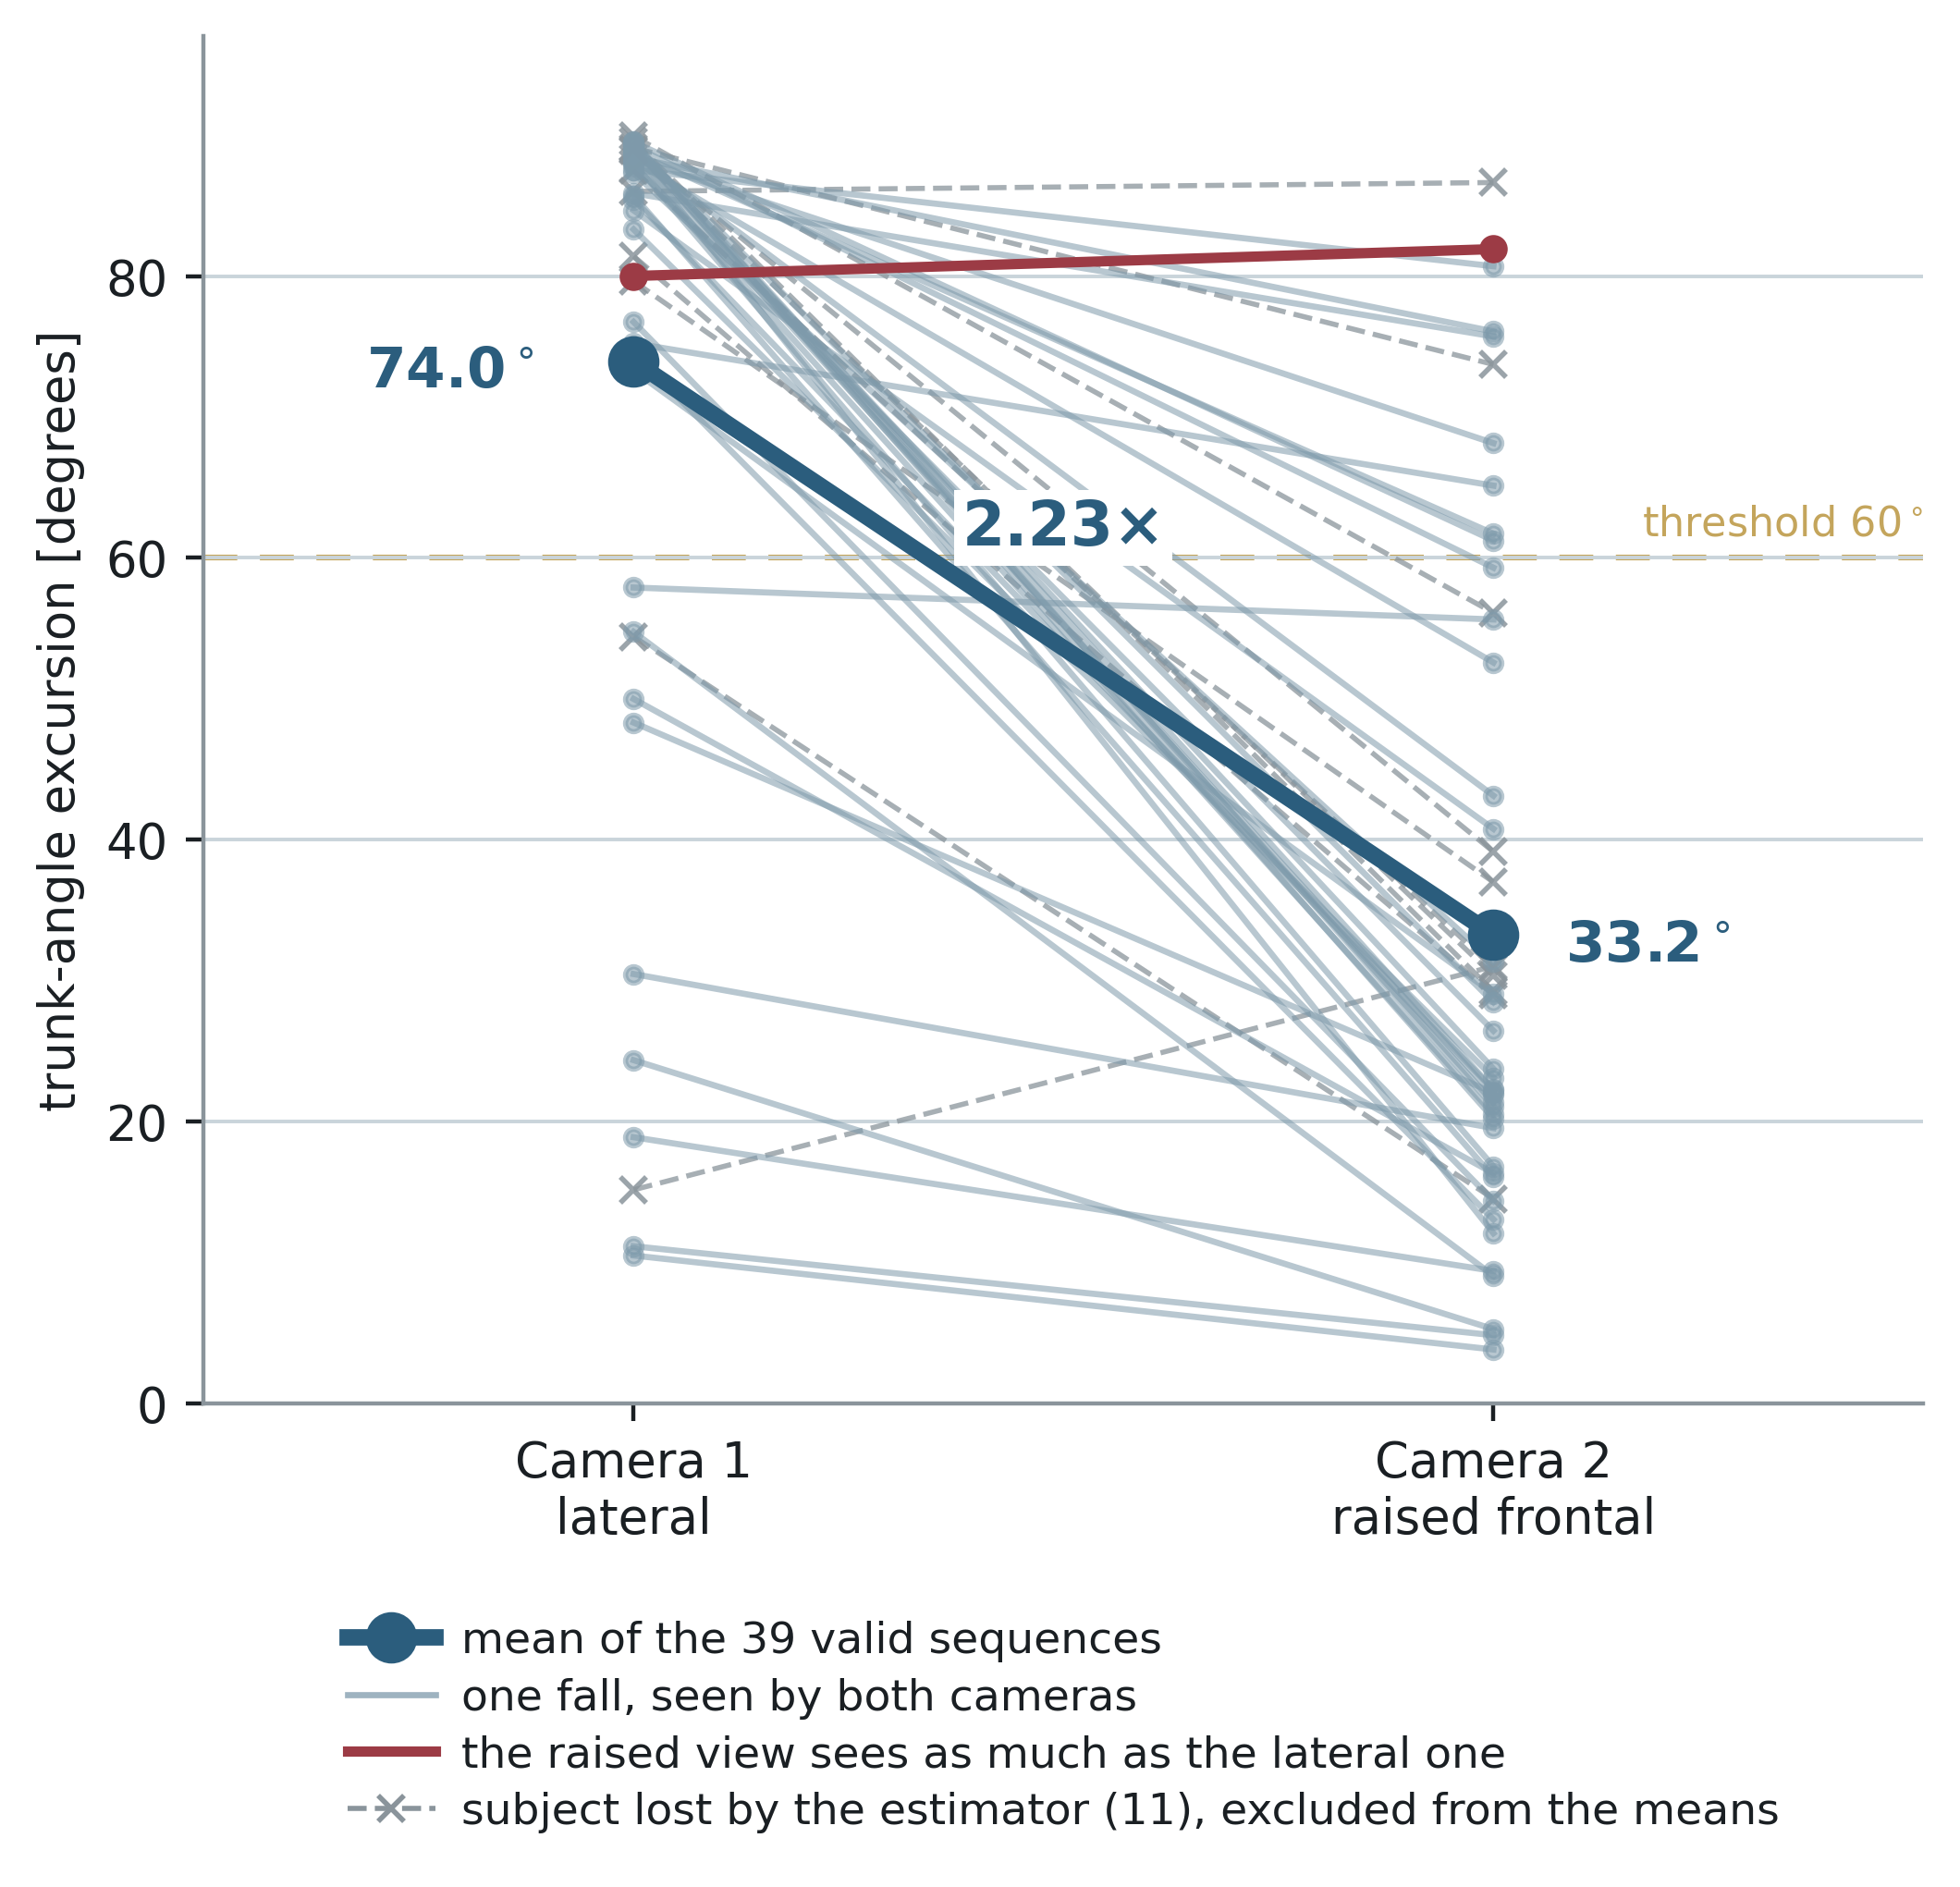
\includegraphics[width=\textwidth]{figure/fig_viewpoint_dist_en.png}
\caption{Excursion of the trunk angle in the two views for the 39 valid sequences.}
\label{fig:viewpoint_dist}
\end{figure}

The geometric difference also appears in the performance of the classifier.

\begin{table}[htbp]
\centering
\caption{Performance as the views used for training and test vary. Representation A3i (twelve quantities, without $h_{\text{pav}}$), random forest, three-class formulation, threshold $0{,}50$.}
\label{tab:viste}
\begin{tabular}{lccc}
\toprule
\textbf{Training} & \textbf{Test} & \textbf{$F_2$} &
\textbf{False positives} \\
\midrule
Camera 1 & Camera 1 & $0{,}822 \pm 0{,}099$ & 722 \\
Camera 1 & Camera 2 & $0{,}488 \pm 0{,}119$ & 3.252 \\
Camera 1 + Camera 2 & Camera 2 & $0{,}731 \pm 0{,}188$ & 751 \\
\midrule
Camera 2 & Camera 2 & $0{,}753 \pm 0{,}179$ & 1.067 \\
\bottomrule
\end{tabular}
\end{table}

\begin{figure}[htbp]
\centering
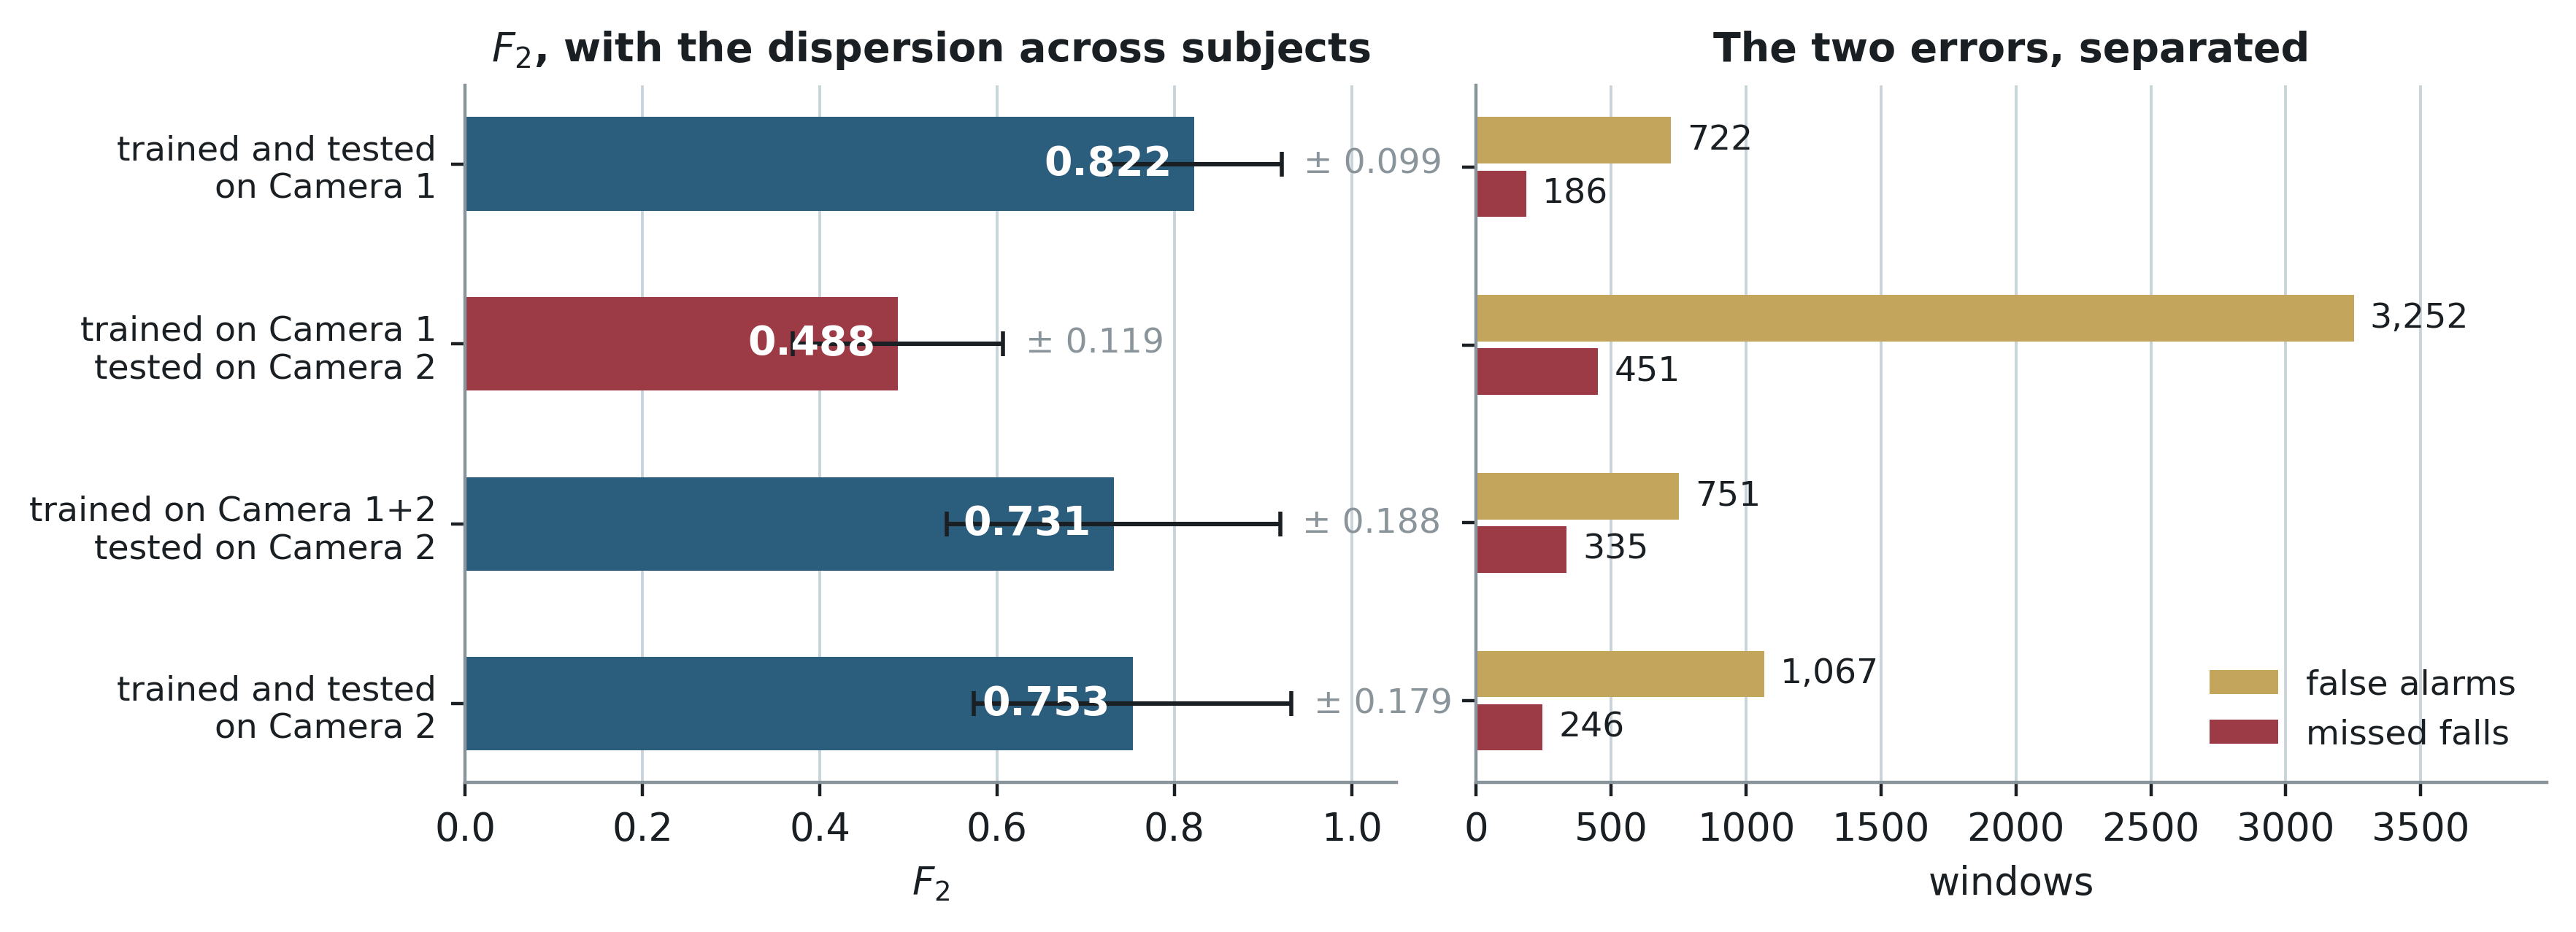
\includegraphics[width=\textwidth]{figure/fig_viste_en.png}
\caption{Performance obtained by changing the view used during training and test.}
\label{fig:viste}
\end{figure}

Training and evaluating the model on Camera~1 gives $F_2=0{,}822\pm0{,}099$. Applying the same model to Camera~2, the value drops to $0{,}488\pm0{,}119$, a loss of 0,334 of $F_2$, about three times the dispersion observed across subjects. The false positives rise at the same time from 722 to 3.252. When both views are included during training, on Camera~2 $F_2$ rises to 0,731 and the false positives fall to 751. Recall and precision also increase, from 0,670 to 0,762 and from 0,316 to 0,713 respectively.

The variability due to the viewpoint can therefore be reduced by including several geometries during training, but a difference with respect to the lateral view remains. An example is shown in Figure~\ref{fig:due_camere}.

\begin{figure}[htbp]
\centering
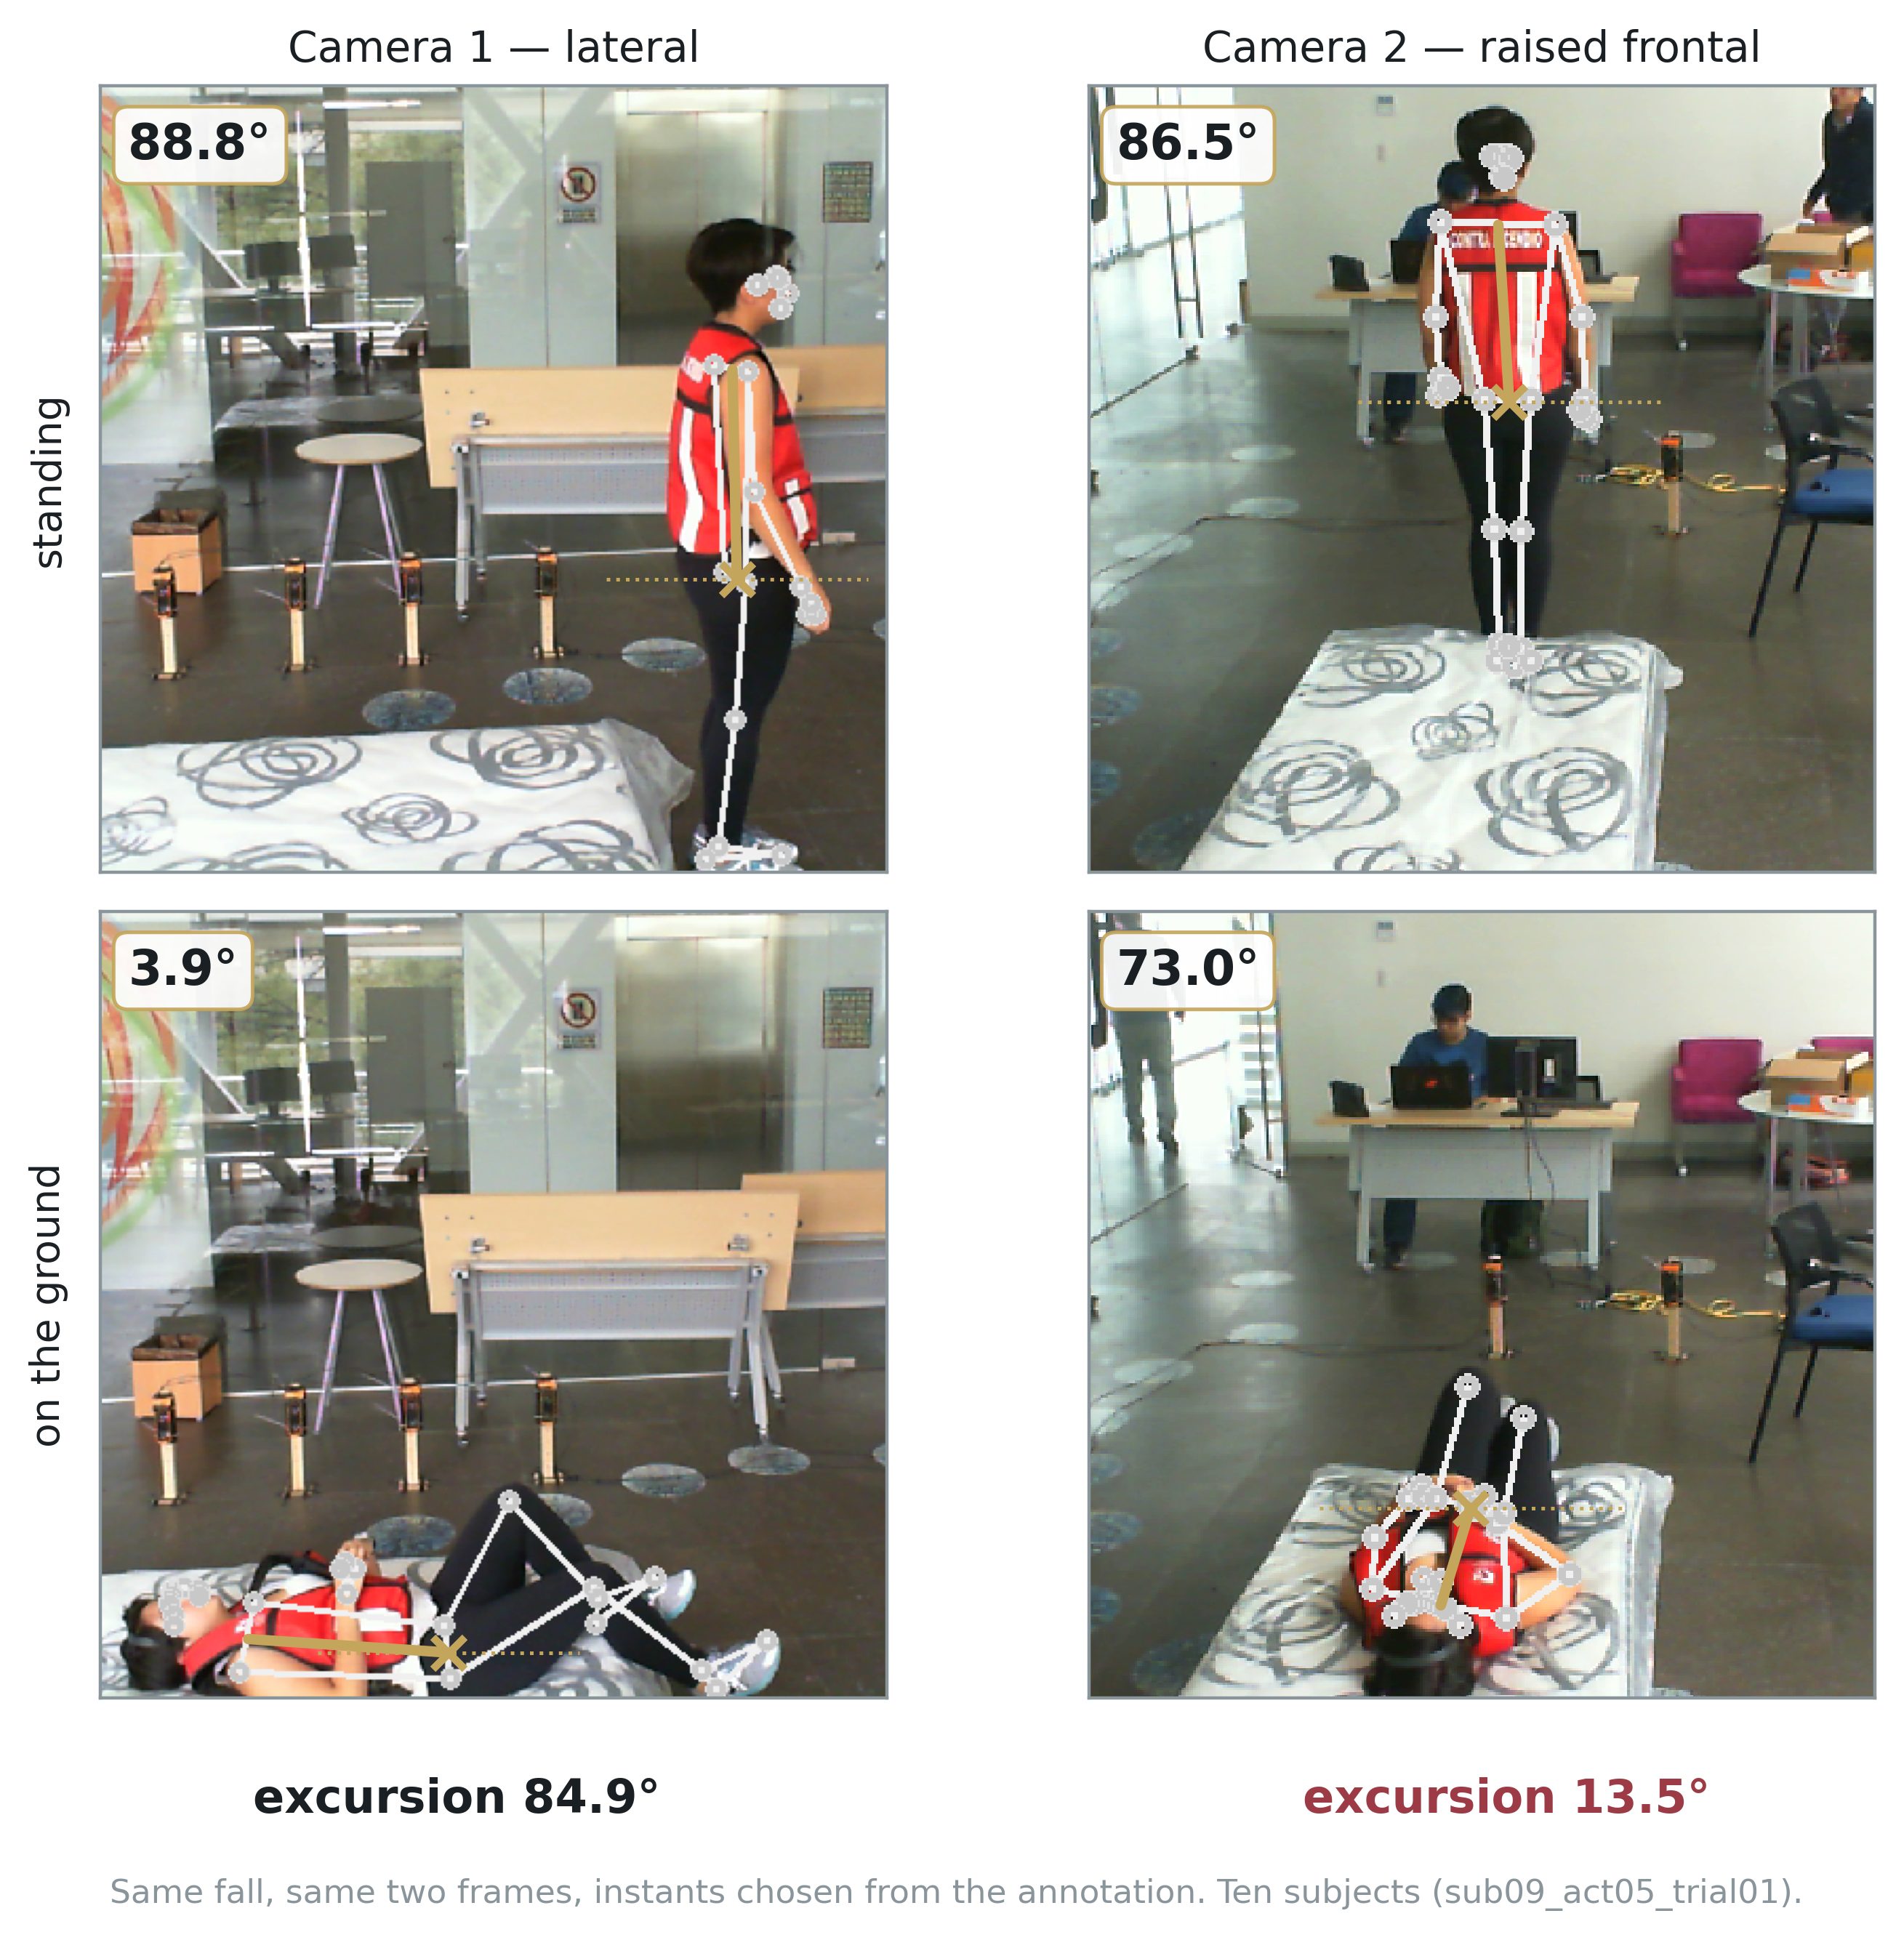
\includegraphics[width=0.85\textwidth]{figure/fig_due_camere_en.png}
\caption{The same fall observed from Camera~1 and from Camera~2. In the lateral view the excursion of the trunk angle is $84,9^\circ$, whereas in the raised frontal view it is $13,5^\circ$.}
\label{fig:due_camere}
\end{figure}

The geometry also changes $h_{\text{pav}}$. The separation between the medians of the two classes is $+1{,}510$ trunk lengths in the lateral view and only $+0{,}060$ in the raised frontal one. The feature therefore loses almost all its separating power when the camera is placed frontally and from above. This is why the criterion of Section~\ref{sec:dtw}, which
considers both cameras, does not include it in the main subset

\subsection{Transfer to an external dataset}
\label{sec:domainshift}

LOSO changes the subject but leaves dataset, environment and acquisition procedure unchanged. In order to assess the behaviour under conditions further from those of training, the model was also applied to UR-Fall, used as an external dataset. With respect to UP-Fall, the subjects, the environment and the recording modalities all change.

The annotations of the two datasets are not directly compatible. UP-Fall distinguishes the fall transition from the post-fall state, whereas UR-Fall describes mainly the posture. UR-Fall is therefore re-extracted with the same pose estimator and the same geometric engine, and the annotations are mapped onto the three phases used in the pipeline. The extraction comprises 11.400 frames distributed over 67 recordings and produces the same 33 candidate features.

The pose is available in 81,0\% of the frames, against 92,3\% for Camera~1 of UP-Fall. Two different trials were carried out on the external dataset. In the direct transfer, model and threshold are kept unchanged. In the diagnostic recalibration the model remains unchanged, while the threshold is recomputed using the labels of UR-Fall. The first experiment therefore measures the actual behaviour of the system on the new dataset. The second serves only to distinguish how much of the loss is due to the calibration of the threshold and how much to a reduction in discriminative power.

\subsubsection{Direct transfer}
\label{sec:esterno}
Since the prevalence of the positive class changes between the datasets, the PR-AUC was also considered, which measures the ability of the classifier to rank the positive windows irrespective of the threshold chosen. For a random classifier the expected PR-AUC coincides with the prevalence. We therefore define

\[
G_{\mathrm{PR}} = \frac{\mathrm{PR\text{-}AUC}} {\mathrm{prevalence}},
\]

Table~\ref{tab:esterno} reports the results obtained on UR-Fall.

\begin{table}[htbp]
\centering
\caption{Transfer from UP-Fall to UR-Fall.}
\label{tab:esterno}
\small
\begin{tabularx}{\textwidth}{@{}Xcccc@{}}
\toprule
\textbf{Configuration} &
\textbf{Prevalence} &
\textbf{PR-AUC} &
\textbf{Gain} &
\textbf{$F_2$ at $\theta=0{,}50$} \\
\midrule
A3 without integrals
& 0,130 & 0,440 & 3,4$\times$ & 0,404 \\
A3 with integrals & 0,130 & 0,466 & 3,6$\times$ & 0,479 \\
DTW subset & 0,130 & 0,660 & 5,1$\times$ & 0,630 \\
\midrule
Previous configuration
& 0,094 & 0,169 & 1,8$\times$ & 0,034 \\
\bottomrule
\end{tabularx}
\end{table}

Among the three directly comparable configurations, the ratio between PR-AUC and prevalence goes from 3,4 for A3 without integrals to 3,6 with the integral quantities, and reaches 5,1 with the subset selected by DTW.

The $F_2$ at the threshold fixed on UP-Fall also increases, from 0,404 to 0,479 and finally to 0,630. The DTW subset therefore retains a greater separating power on the external dataset than the other two configurations, while still showing a degradation with respect to the training domain. The previous configuration uses a different definition of the positive and a prevalence of 0,094. Its gain is therefore not directly comparable with the other three and is reported as a point of reference.

\begin{figure}[htbp]
\centering
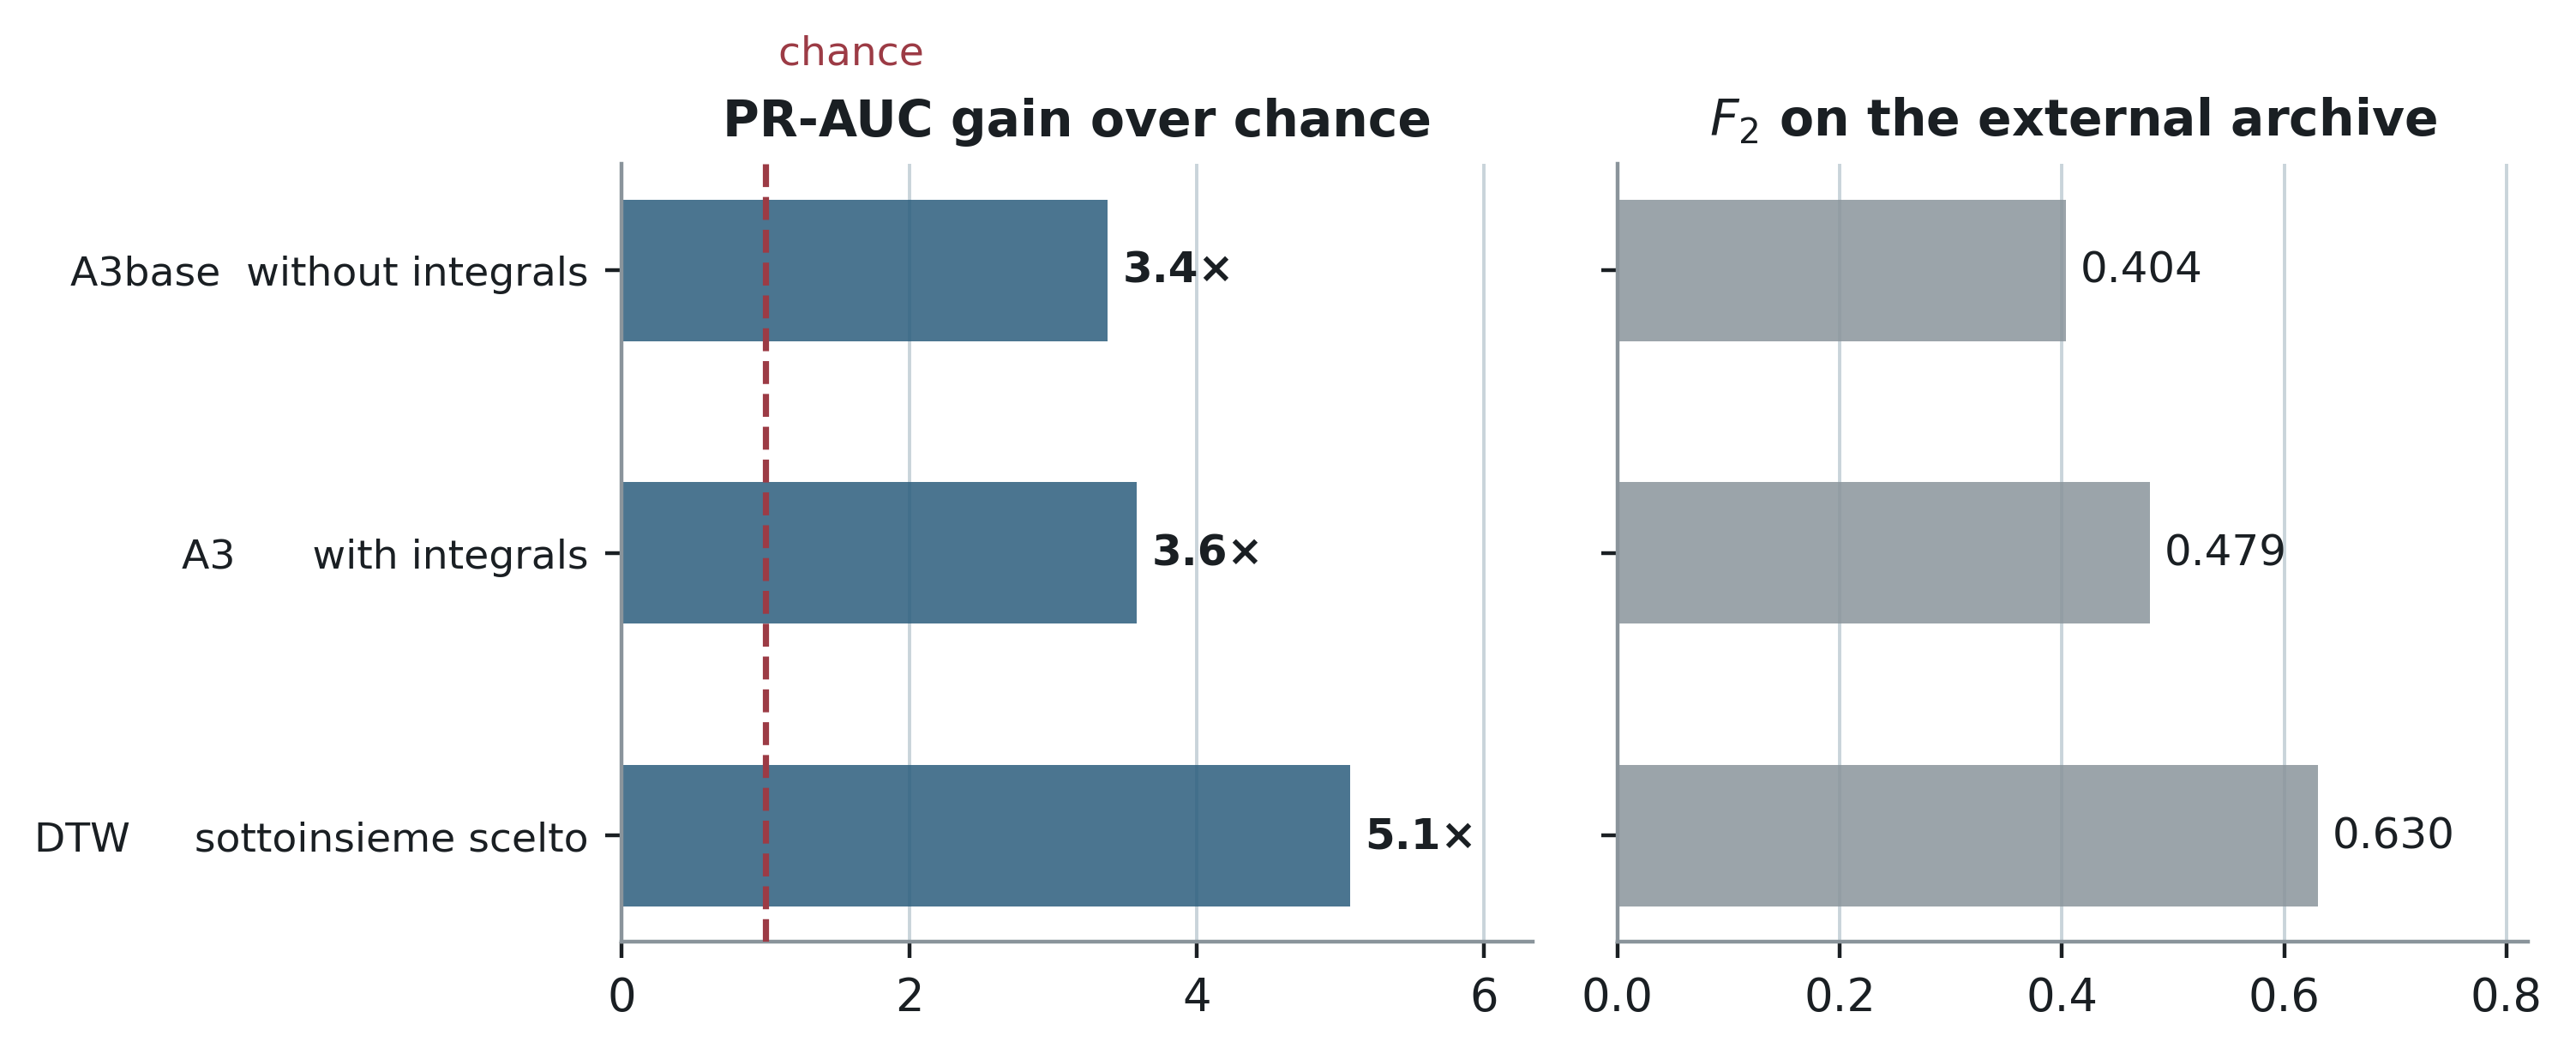
\includegraphics[width=0.85\textwidth]{figure/fig_esterno_en.png}
\caption{Performance in the transfer to UR-Fall. On the left the ratio between PR-AUC and prevalence is reported, while on the right the $F_2$ obtained with the threshold fixed on the source dataset is shown.}
\label{fig:esterno}
\end{figure}

\subsubsection{Diagnostic recalibration}

The degradation on an external dataset may depend on two different phenomena. The first is a loss of calibration: the model retains part of its ability to rank the windows, but produces scores on a different scale. The second is a loss of discriminative power: the two classes become harder to separate. In order to distinguish the two effects, a second trial was carried out on the previous configuration, recomputing the threshold that maximises $F_2$ directly on UR-Fall.

This threshold uses the labels of the target dataset and is therefore called the \emph{oracle threshold}. It does not represent a procedure usable in a real installation, because it requires knowing in advance the labels of the data to which the system is to be applied.

\begin{figure}[htbp]
\centering
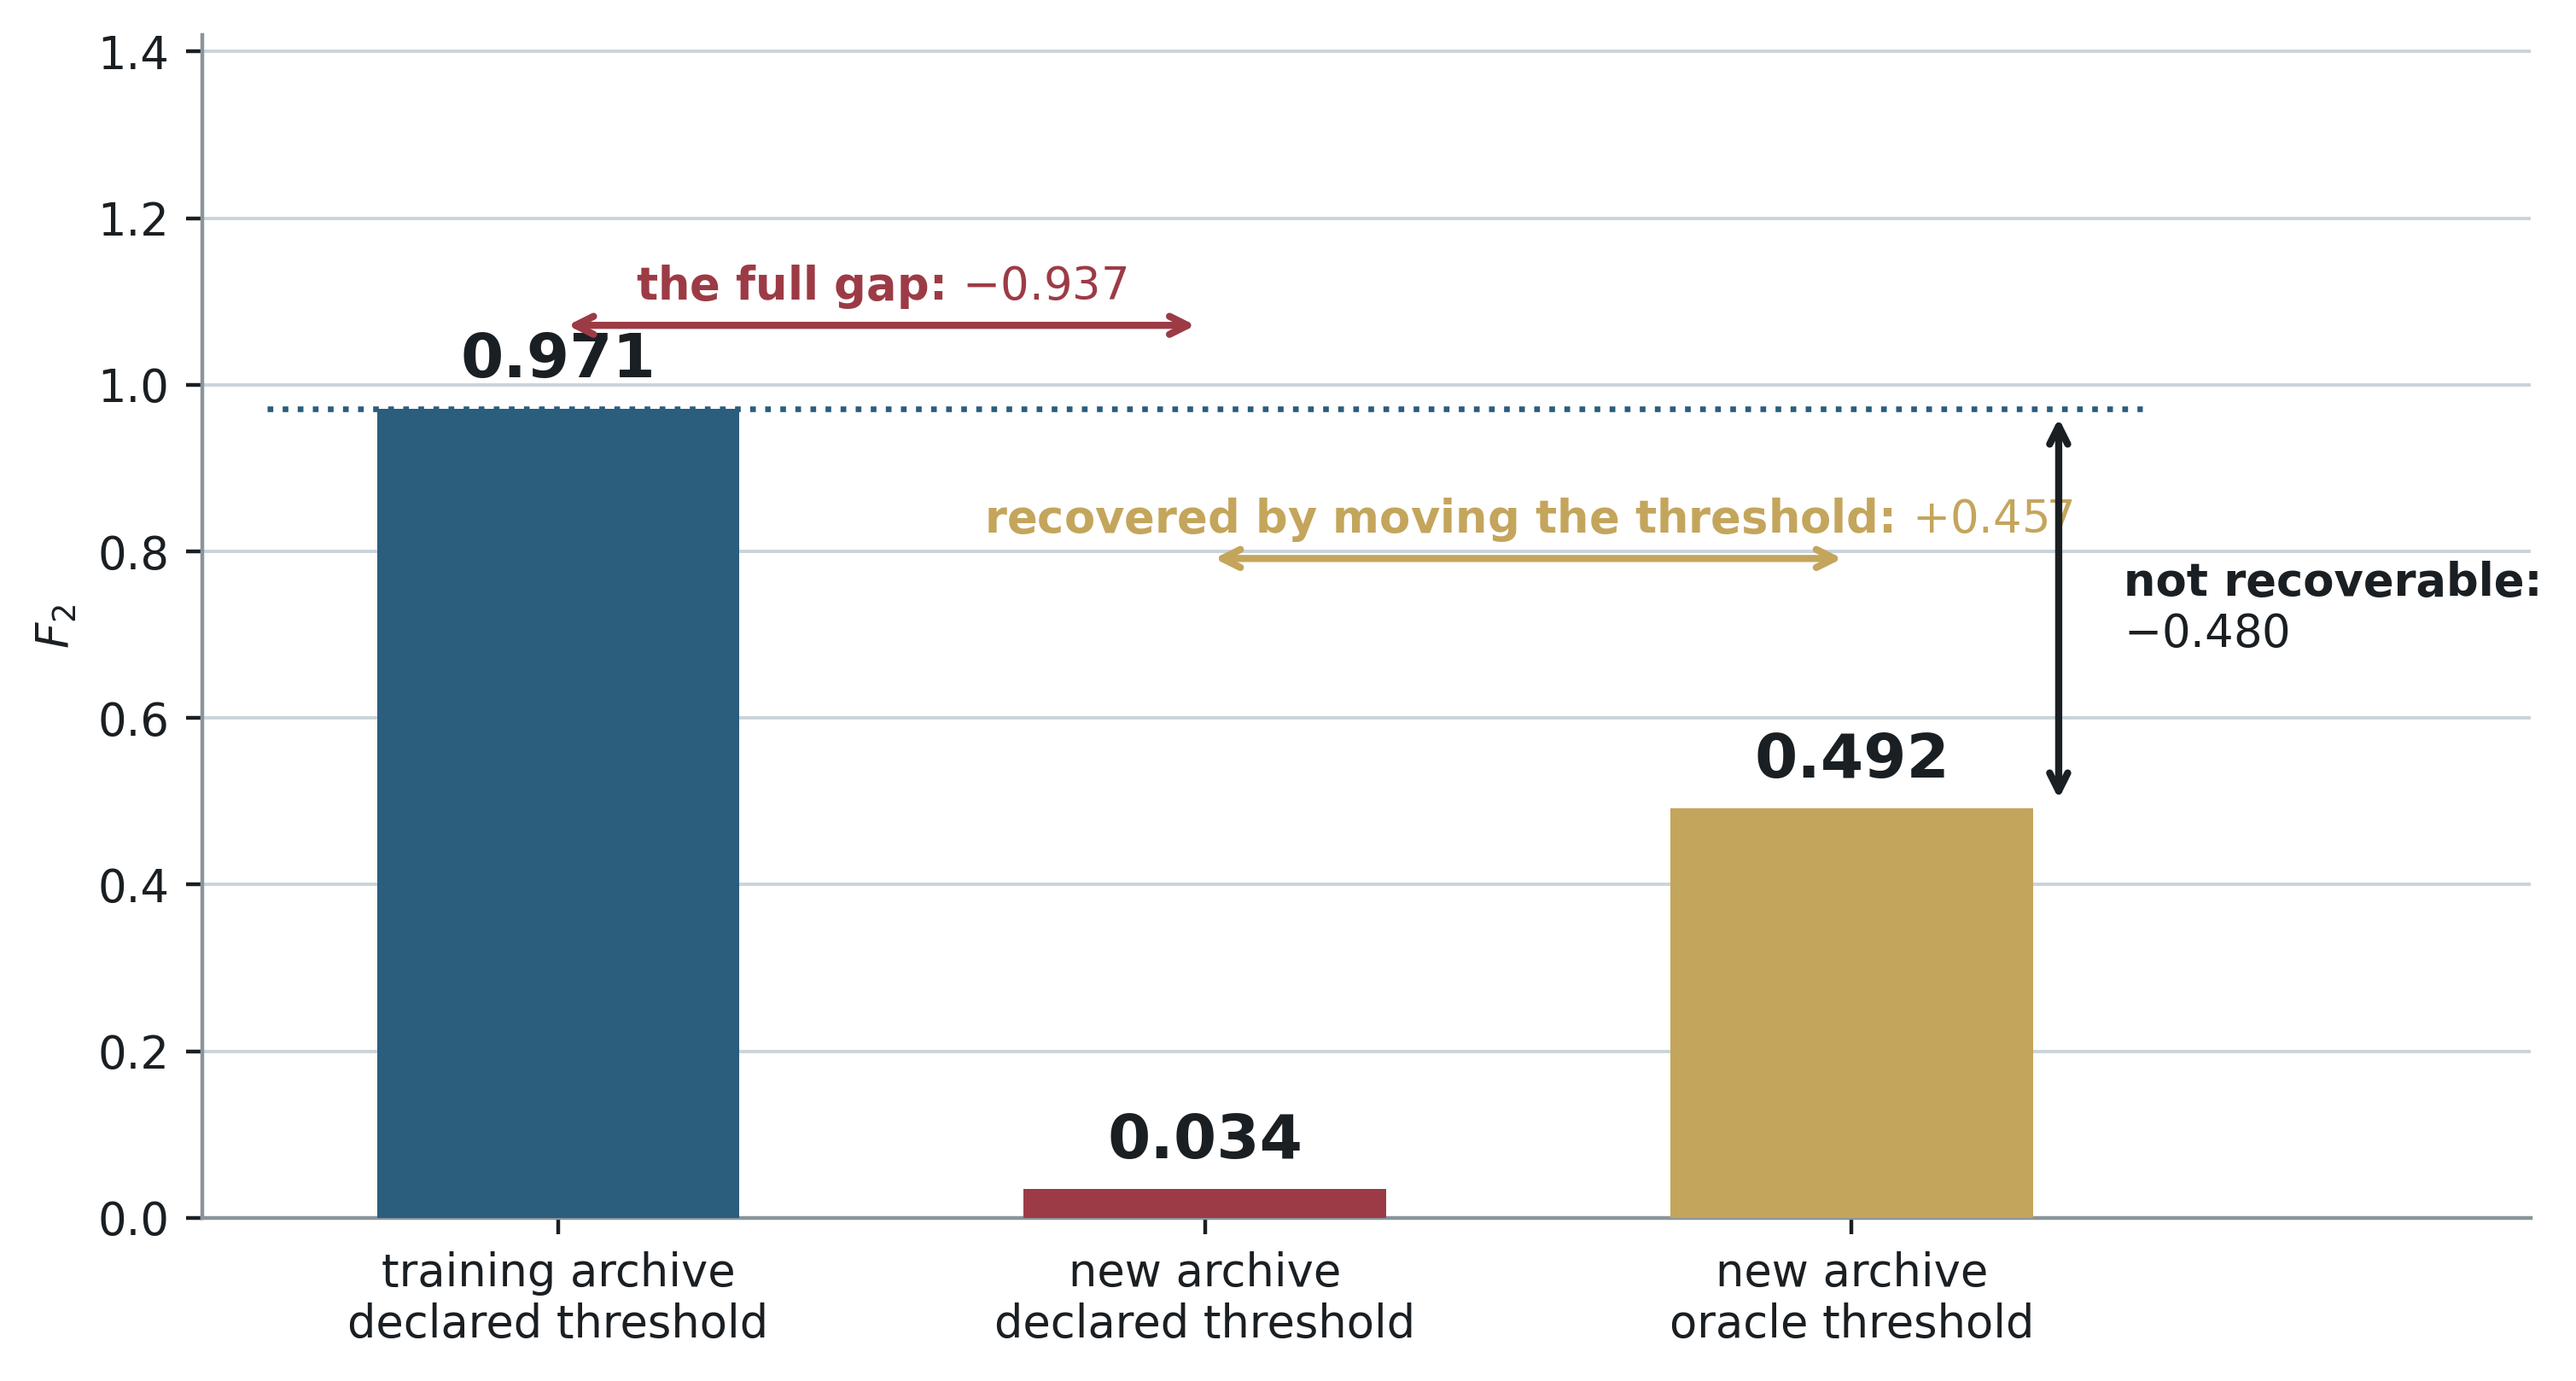
\includegraphics[width=0.85\textwidth]{figure/fig_dominio_en.png}
\caption{Decomposition of the gap between the source domain and UR-Fall into loss of calibration and loss of discriminative power.}
\label{fig:dominio}
\end{figure}

With the threshold fixed on UP-Fall, the previous configuration obtains $F_2=0,034$ on UR-Fall. With the oracle threshold the value rises to 0,492. In the source domain the same configuration reached about 0,971. Of the 0,937 points of difference, about 0,457 are recovered by changing the threshold, while about 0,480 remain even after recalibration.

The drop therefore does not depend on the threshold alone. Even after the decision point has been adapted, a substantial loss of discriminative power remains. The same conclusion is consistent with the PR-AUC: in the previous configuration the ratio with respect to the prevalence goes from about 18,7 in the source domain to 1,79 on UR-Fall. This decomposition was carried out only on the previous configuration and must not be attributed directly to the DTW subset. For the latter the direct transfer is available, with a PR-AUC of 0,660 and $F_2=0{,}630$ at the threshold fixed at 0,50.

A loss of calibration can be addressed by changing the decision
threshold, whereas a loss of discriminative power requires
intervening on the model or on the data used to train it. Supervised recalibration would in any case require labelled examples from the new environment, which are not normally available at the time of installation. The oracle threshold is therefore used only as a diagnostic tool and not as a level of performance actually achievable by the system on the external dataset.

\chapter{Implementation on an edge device and validation in a real environment}
\label{cap:edge}

In Chapter~\ref{cap:sperimentale} the system was evaluated on recordings already available, without imposing any constraint on the time needed to process each frame. In this chapter we shall instead verify the operation of the whole pipeline, analysing the porting to a Radxa ROCK 4D, the computational cost and the choice of the operating configuration. We shall then move to a real environment and analyse the domestic acquisitions, evaluating the system during prolonged operation and in the passage from metrics on the individual windows to alarm events.

\section{Edge platform and operating configuration}
\label{sec:piattaforma}

A \textbf{Radxa ROCK 4D} with a Rockchip RK3576 SoC, 6~GB of memory and an integrated 6~TOPS NPU was used for the implementation. The overall cost of the platform, USB camera included, is of the order of a hundred euros per acquisition point.
Unlike a centralised architecture, in which one or more cameras send the images to an external server, here the whole pipeline is executed locally: acquisition, pose estimation, feature extraction and classification. Only the information associated with a possible alarm is transmitted outside.

\begin{table}[htbp]
\centering
\caption{Comparison between local processing on an edge device and the use of a remote server.}
\label{tab:edge_vs_server}
\begin{tabularx}{\textwidth}{@{}lXX@{}}
\toprule
& \textbf{Edge node} & \textbf{Server with GPU} \\
\midrule
Computation & ARM SoC + NPU & x86 CPU + dedicated GPU \\
Cost & per node & shared infrastructure \\
Network required & not necessary & necessary \\
Data transmitted & alarm information & video stream \\
\bottomrule
\end{tabularx}
\end{table}

The main difference concerns the \textbf{cost per room}. A server can be shared between several cameras, but requires each of them to transmit its own video stream continuously. This reduces the computational cost per individual room, but increases the dependence on the network and the data have to leave the home. An edge node dedicated to each room does not enjoy the same economy of scale, but has a known cost per installation and keeps the processing and the data local, as required in Chapter~\ref{cap:contesto}.

\subsection{Porting constraints}

Three main problems emerged during the porting.

The first concerns the architecture of the processor. The more recent versions of MediaPipe tried on the board are compiled for ARMv8.1, whereas the RK3576 implements ARMv8.0. Execution terminated with an \texttt{illegal instruction} error. Version 0.10.9 works correctly and was therefore retained.

The second problem concerns the interface used by the code. The more recent versions of MediaPipe have progressively replaced the \texttt{mp.solutions} interface, on which the feature extraction pipeline had been built. Changing interface would have required modifying a significant part of the code already used in the earlier experiments. This too is a reason why the version compatible with the existing pipeline was retained.

The third problem emerged during the trials with the NPU. The converted model requires a four-dimensional input tensor. With a three-dimensional tensor the inference was not executed, but no explicit error was returned. The time measured therefore came out very low without the model having actually processed the data. From this trial onwards it was verified that the computation was really being carried out and that the output was correct before any speed measurement was used.

\section{Verification of equivalence between computer and device}
\label{sec:parita}

Before measuring performance on the board, it was verified that the classifier produced the same results as those obtained on the computer.
The first trial was carried out on 200 windows already computed, thereby excluding the camera and the pose estimator.

\begin{table}[htbp]
\centering
\caption{Comparison of the predictions on 200 precomputed windows.}
\label{tab:parita}
\begin{tabular}{lr}
\toprule
Maximum discrepancy between the predictions & $2{,}2\times10^{-16}$ \\
Differing decisions & 0 \\
\bottomrule
\end{tabular}
\end{table}

No differing decisions were observed. At parity of features, normalisation and classifier, the two systems therefore produce the same result. The comparison was then repeated starting directly from the videos. Out of 56 clips, 55 produced the same final decision. In one recording alone, containing a fall, the decision turned out different.
The difference arises before the classifier. MediaPipe maintains a temporal state in order to follow the person, and small variations in the landmarks change the features obtained. When the score is close to the threshold, this variation can change the final decision.

Some faulty measurements were identified during these tests. In one trial different models showed almost identical times because no person was detected in the frames used. In another trial about 1.315~fps were measured because the inference on the NPU was not being executed, owing to the wrong input shape.
An early check on the landmarks was also too weak: it verified only that the coordinates were positive, and therefore treated as valid even points that were clearly placed wrongly. The measurements reported in the following sections are therefore used only after both the execution of the computation and the consistency of the output have been checked.

\subsection{Comparison between pose estimators}
\label{sec:stimatore}

Pose estimation is the most expensive stage of the pipeline. MediaPipe on the CPU of the Radxa takes about 92,6~ms per frame, that is 10,8~fps. It is therefore not possible to keep the 18~fps of the original dataset. In order to increase the speed, YOLOv8-pose quantised to INT8 and run on the NPU was tried.

The inference alone turns out to be 5,16 times faster. The gain for the whole pipeline was initially 1,71 times, because the post-processing took 12,14~ms per frame. After this part of the code had been vectorised, the time dropped to 0,94~ms and the overall gain rose to 2,17 times.
Speed alone is not, however, enough. The quality of the pose was therefore verified over 29.681 frames belonging to different activities.

\begin{table}[htbp]
\centering
\caption{Pose retention with YOLOv8-pose INT8 and MediaPipe. Five-subject experiment.} \label{tab:ritenzione}
\begin{tabular}{lcc}
\toprule
\textbf{Activity} & \textbf{YOLOv8 INT8} & \textbf{MediaPipe} \\
\midrule Standing, sitting down, picking up, jumping & 100\% & 100\% \\
Forward fall onto the hands & 79,2\% & 99,5\% \\
\textbf{Lying down} & \textbf{43,6\%} & \textbf{79,1\%} \\
\bottomrule
\end{tabular}
\end{table}

The difference appears above all when the person is close to the floor. For the lying position, YOLOv8 keeps the detection in 43,6\% of the frames against 79,1\% for MediaPipe. Lowering the YOLOv8 threshold to 0,05 brings it to 58,9\%, still below MediaPipe.

A difference in the estimated geometry was also observed. With YOLOv8 the projected length of the torso goes from 83,5 pixels when standing to 56,5 pixels on the ground. With MediaPipe it goes instead from 83,8 to 100,7 pixels. This quantity is used in the body-centric normalisation. An error in the length of the torso therefore changes several features at once. In order to measure the final effect, the two estimators were compared while features, classifier, threshold and protocol were kept unchanged.

\begin{table}[H]
\centering
\caption{Performance obtained by replacing the pose estimator. Five-subject experiment.}
\label{tab:stimatori_f2}
\begin{tabular}{lccc}
\toprule
\textbf{Estimator} & \textbf{$F_2$} & \textbf{FP} & \textbf{FN} \\
\midrule MediaPipe & $0{,}909 \pm 0{,}095$ & 17 & 23 \\
YOLOv8 INT8 & $0{,}682 \pm 0{,}044$ & 225 & 59 \\
\bottomrule
\end{tabular}
\end{table}

The mean difference of $F_2$ is 0,227, and YOLOv8 increases both the false positives and the false negatives. These values come from the five-subject experimental configuration and were not repeated after the extension to ten subjects. They are therefore used as indicative results for the choice of the estimator, whereas the timing measurements were obtained directly on the board.

\subsection{Choice of the operating configuration}
\label{sec:decisione}

The final choice must hold together processing frequency and quality of the pose. The Random Forest was used on the board. In the tests of Chapter~\ref{cap:sperimentale} some neural networks obtain slightly better results, but the differences between the main architectures remain small with respect to the variability observed between subjects. The Random Forest was therefore preferred because it is simpler to run on the device, does not require the TensorFlow stack and reduces the software dependencies of the pipeline.

\begin{table}[htbp]
\centering
\caption{Configurations considered for operation on the device.}
\label{tab:catene}
\begin{tabular}{llccc}
\toprule \textbf{Configuration} & \textbf{On the device} & \textbf{$F_2$} & \textbf{FP} & \textbf{FN} \\
\midrule
MediaPipe @ 18 fps & not attainable & 0,898 & 23 & 24 \\
MediaPipe @ 9 fps & 10,8 fps & 0,857 & 57 & 49 \\
YOLOv8 @ 18 fps & 26,5 fps & 0,682 & 225 & 59 \\
\bottomrule
\end{tabular}
\end{table}

MediaPipe at 18~fps is not usable on the board, but it reaches 10,8~fps and can therefore be used with a sequence subsampled to 9 samples per second. Moreover, of the two configurations that can actually be run, MediaPipe at 9~fps keeps the better results: $F_2=0{,}857$ against 0,682 for YOLOv8, while recall is 0,866 and 0,775 respectively. The number of errors is lower as well: 49 false negatives and 57 false positives with MediaPipe, against 59 and 225 with YOLOv8.

\begin{table}[htbp]
\centering
\caption{Variation of $F_2$ associated with subsampling and with the change of pose estimator.}
\label{tab:scomposizione}
\begin{tabular}{lr}
\toprule
\textbf{Change} & \textbf{$\Delta F_2$} \\
\midrule MediaPipe from 18 to 9 fps & $-0{,}041$ \\
MediaPipe $\rightarrow$ YOLOv8 INT8 & $-0{,}216$ \\
\midrule Ratio between the variations & $5{,}3\times$ \\
\bottomrule
\end{tabular}
\end{table}

In the comparison carried out, changing estimator costs about five times more than halving the frequency. MediaPipe was therefore retained, and the model intended for the board was trained at 9 samples per second.
Subsampling does nonetheless have a cost, reported in Table~\ref{tab:catene}: the false negatives go from 24 to 49 and $F_2$ drops by $0{,}041$. YOLOv8 was evaluated only in the INT8 version. It is therefore not possible to separate the effect of the network from that of the quantisation.

The NPU remains useful from a computational point of view: the inference of YOLOv8-pose is 5,16 times faster and, after the post-processing has been optimised, the pipeline reaches 26,5~fps. The limitation observed in this trial therefore concerns the quality of the estimator used, not the capability of the accelerator.

\section{Computational performance and continuity of operation}

Once the configuration had been chosen, the cost of the various stages and the behaviour of the board during prolonged trials were measured.

\subsection{Computational cost and processing frequency}
\label{sec:costo-computazionale}

In order to assess the computational cost, two cases were considered separately: the accelerated chain with YOLOv8-pose on the NPU, shown in Table~\ref{tab:costo}, and the configuration actually installed, based on MediaPipe on the CPU.

\begin{table}[htbp]
\centering
\caption{Cost per frame of the accelerated chain with YOLOv8-pose on the NPU.}
\label{tab:costo}
\begin{tabular}{lrr}
\toprule
\textbf{Stage} & \textbf{Time} & \textbf{Share} \\
\midrule
Pre-processing & 1,21 ms & 3,2\% \\
Perception & 33,34 ms & 88,4\% \\
Post-processing & 0,94 ms & 2,5\% \\
Classification, amortised cost & 2,21 ms & 5,9\% \\
\midrule
Total & 37,7 ms & 100\% \\
\bottomrule
\end{tabular}
\end{table}

The overall time is about 37,7~ms per frame, corresponding to 26,5~fps. This configuration is not, however, the one used in the domestic trials. The figure does show that the dominant stage remains pose estimation, which takes up 88,4\% of the total time. The values for the accelerated chain come from a dedicated benchmark and were initially transcribed from the terminal. The measurement was not subsequently repeated with the same automatic instrumentation used for the installed chain. This constitutes a limitation on the reproducibility of the measurement.

The configuration actually installed uses MediaPipe on the CPU instead. The times were measured directly on the board during the continuous session of 6 September, lasting 4,59~hours, and are reported in Table~\ref{tab:costo_installato}.

\begin{table}[htbp]
\centering
\caption{Cost per frame of the installed configuration.}
\label{tab:costo_installato}
\begin{tabularx}{\textwidth}{Xrrr}
\toprule
\textbf{Stage} & \textbf{Time} & \textbf{Share} & \textbf{Accelerated chain} \\
\midrule
Perception & 116,38 ms & 85,2\% & 33,34 ms \\
Classification, amortised cost & 19,51 ms & 14,3\% & 2,21 ms \\
Other operations & 0,76 ms & 0,6\% & 2,15 ms \\
\midrule
Total & 136,65 ms & 100\% & 37,7 ms \\
Frequency & 7,3 fps & & 26,5 fps \\
\bottomrule
\end{tabularx}

\end{table}

On the board the Random Forest takes 39,04~ms to classify a window. Since one decision is produced every two frames, the mean cost is 19,51~ms per frame. The remaining 0,76~ms cover the operations not included in the perception and classification measurements, such as frame acquisition, format conversion, buffer updating and data logging.

For the accelerated chain the item ``other operations'' instead collects pre-processing and post-processing, amounting to $1{,}21+0{,}94=2{,}15$~ms.
In both configurations the bottleneck remains perception: 88,4\% of the time in the accelerated chain and 85,2\% in the installed one. Changing the classifier would therefore have a limited effect on the overall frequency.

The mean time of 136,65~ms corresponds to about 7,3~fps. The real frequency is not, however, constant: across the twelve domestic sessions it ranges between 1,15 and 8,20~fps, while in the two prolonged trials it is 7,26 and 6,47~fps. This variability also changes the temporal duration of the windows. The 22 samples used by the classifier correspond to 2,44~s at the design frequency of 9~fps, but to about 3,40~s when the frequency drops to 6,47~fps. During execution the same window may therefore represent a longer time interval than the one used during training.

\subsection{Thermal stability and prolonged operation}
\label{sec:continuita}

Besides processing speed, the ability of the
device to operate continuously without an evident reduction in performance due to temperature was verified. A first ten-minute trial was carried out, for a total of 18.291 inferences.
The variation in latency between the beginning and the end was 3,9\%. The frequency of the accelerator remained at 950~MHz and the temperature settled between 60 and 63~$^\circ$C.

A second check was obtained during the prolonged domestic session of 11 August, which lasted 6,11~hours of wall clock. This session is used here for the thermal measurement alone, and is not the reference continuous trial: the operating system suspended it for about 68 minutes, so that the effective operating time was 4,99~hours, and the dual-clock check that makes such an interruption detectable was introduced only afterwards. The maximum temperature recorded was 79,5~$^\circ$C and it settled after about forty minutes. No sudden drops in the frame rate attributable to \emph{thermal throttling} were observed.

\begin{figure}[H]
\centering
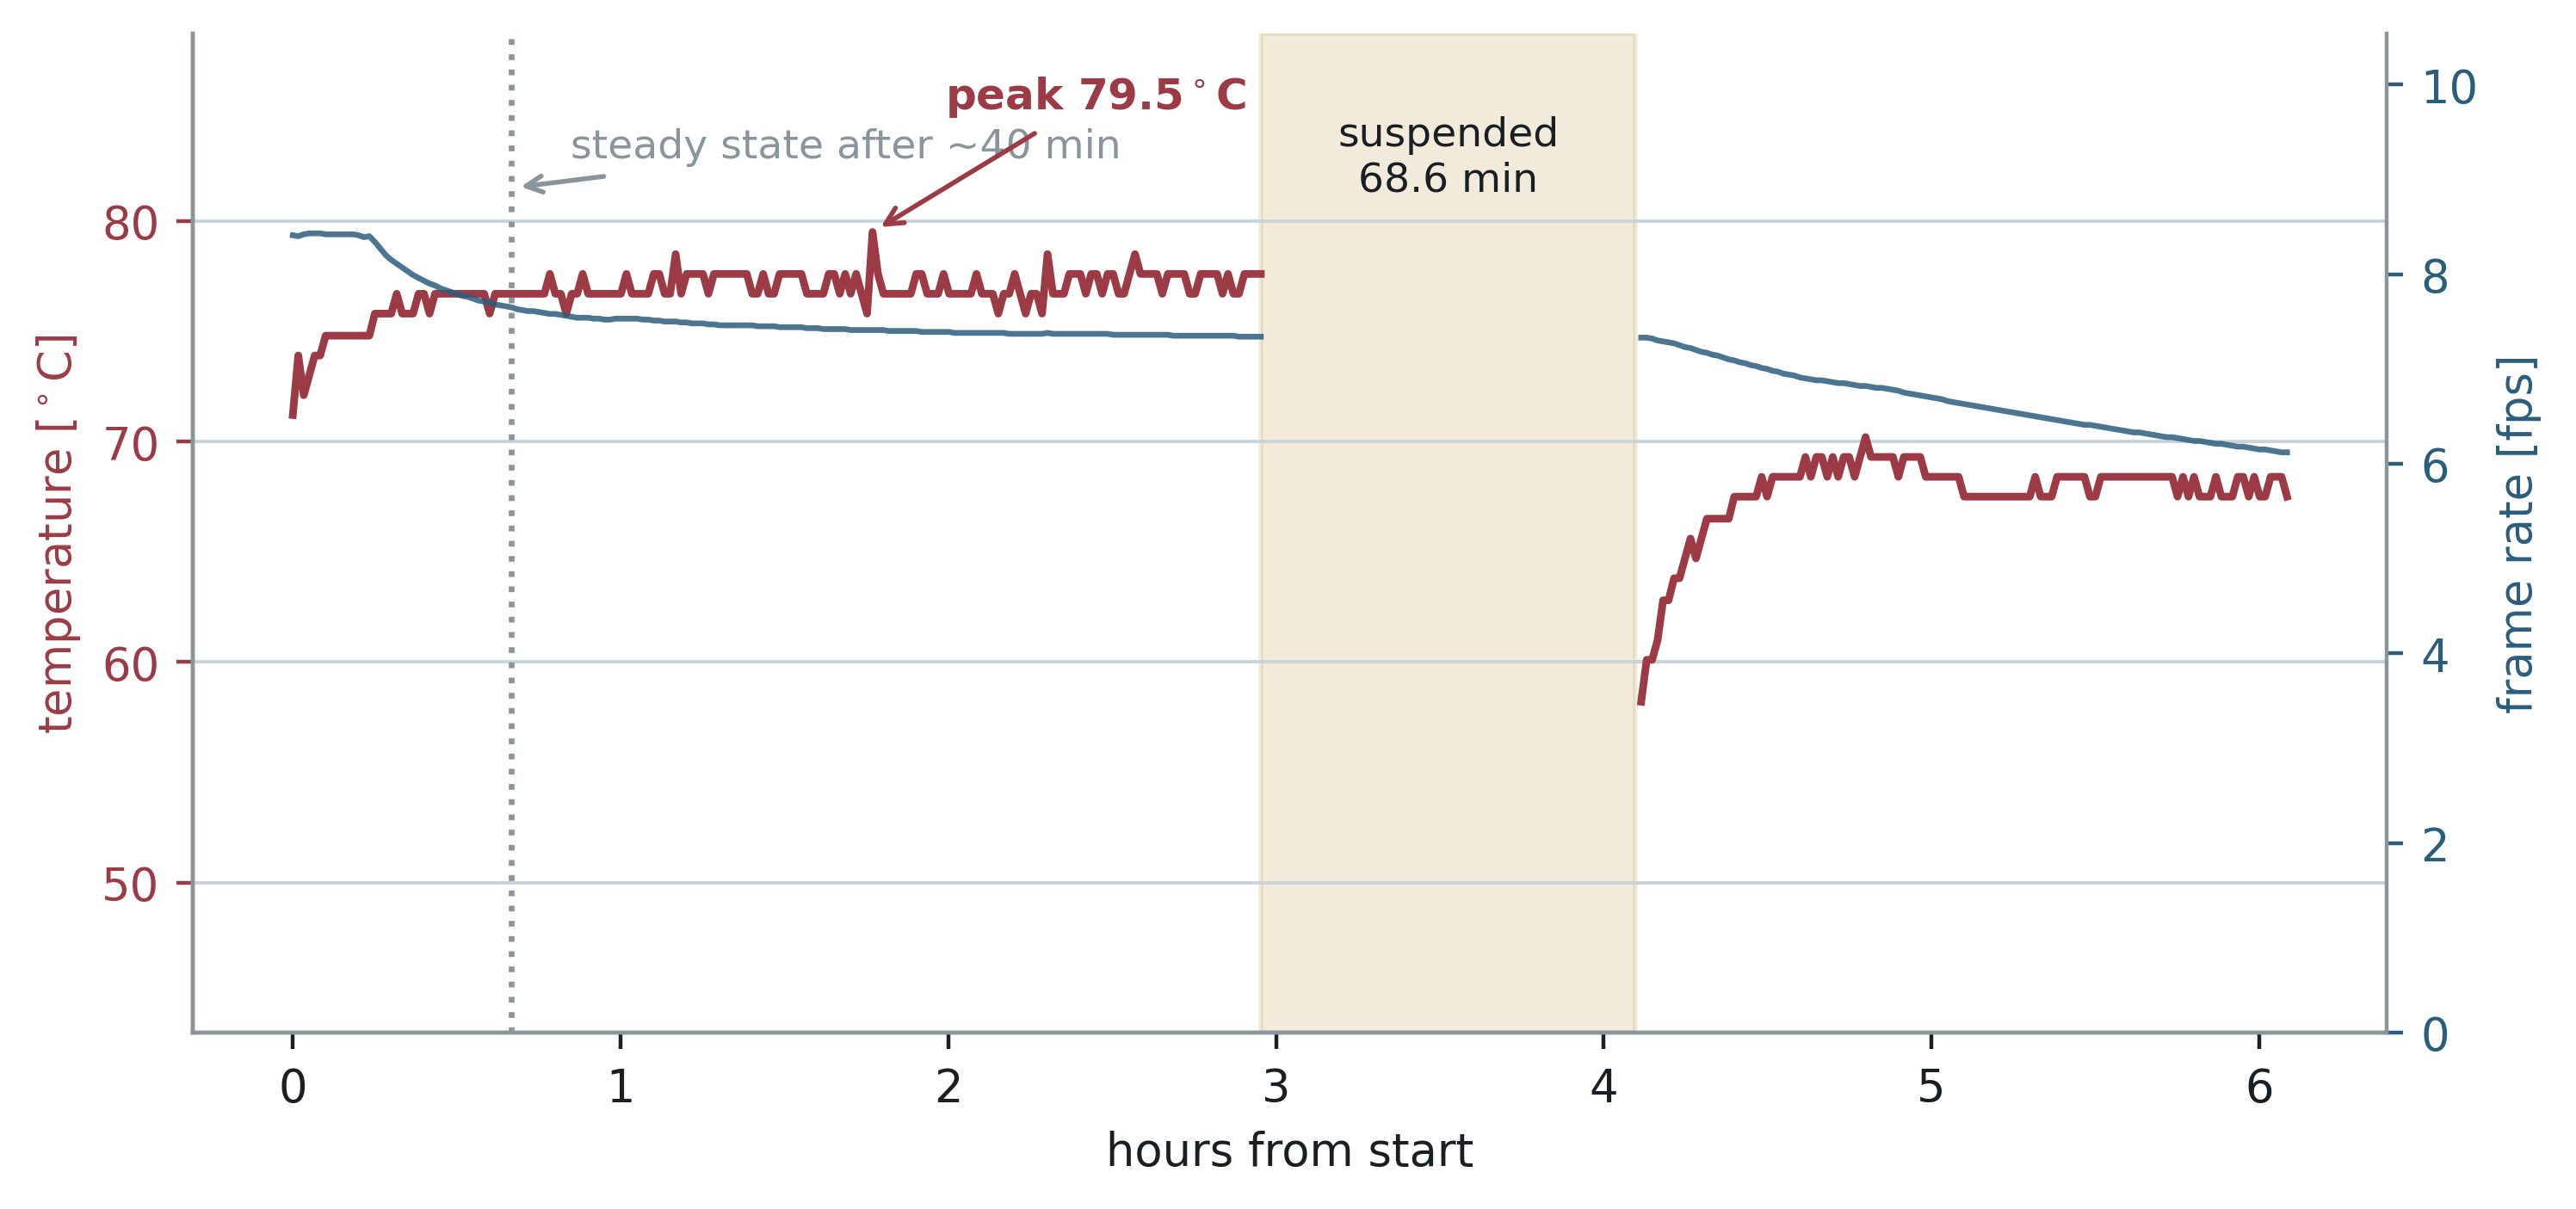
\includegraphics[width=0.85\textwidth]{figure/fig_termica_en.png}
\caption{Temperature of the device and processing cadence during the
prolonged domestic session of 11~August.}
\label{fig:termica}
\end{figure}

During this session, however, the operating system suspended for about 68 minutes. The program did not terminate and resumed execution after the wake-up. In order to make this problem observable, a check based on the comparison between system time and monotonic time was added.

It was moreover observed that the USB camera can be renumbered by the operating system, for example from \texttt{/dev/video0} to \texttt{/dev/video1}. In this case the program may remain active without receiving new frames. Capture is therefore monitored separately and, if no new frame arrives for more than 20~s, the camera is reopened.

A later trial, carried out on 6 September, covered 4,59~continuous hours. No suspensions of the operating system were detected. The camera dropped out twice, for about five seconds in total, and was reopened automatically. The mean cadence was 7,26~fps.

During this trial the system produced 14 events. They are not, however, counted as false alarms, because in that version of the recorder the frames around the alerts were not yet being retained, and it is therefore not possible to verify what actually happened. The 4,59-hour trial does not cover a whole night and therefore cannot demonstrate twelve hours of continuous operation.

\subsection{Resource budget}
\label{sec:risorse}

In Chapter~\ref{cap:contesto} computational and economic sustainability was listed among the requirements of the system. Table~\ref{tab:risorse} summarises the main resources demanded by the platform used.

\begin{table}[htbp]
\centering
\caption{Resource budget of the installed system.}
\label{tab:risorse}
\begin{tabular}{@{}p{4.6cm}p{9.0cm}@{}}
\toprule
\textbf{Quantity} & \textbf{Value} \\
\midrule
Platform & Radxa ROCK 4D, Rockchip RK3576 SoC \\
Memory available & 5.923~MB (6~GB nominal) \\
Accelerator & integrated NPU, 6~TOPS \\
Cost & of the order of 100~\euro{} per room, USB camera included \\
Model size & 606.409~bytes for the classifier, 1.175~bytes for the scaler; 607.584~bytes for everything needed to run \\
Cost per frame & Section~\ref{sec:costo-computazionale} \\
CPU / NPU split & Section~\ref{sec:stimatore} \\
Continuity of operation & Section~\ref{sec:continuita} \\
Memory used by the process & \textbf{297~MB} peak, that is 5\% of the memory available \\
\midrule
\textbf{Power consumption} & \textbf{not measured} \\
\bottomrule
\end{tabular}
\end{table}

The peak memory of the complete process is 297~MB, about 5\% of the memory available. Memory is therefore not a limitation for running the pipeline. The classifier is small as well, about 0,6~MB. The main computational cost therefore remains tied above all to pose estimation.

Power consumption was not measured. This quantity would require a direct measurement of the current drawn during operation and cannot be derived reliably from the specifications of the board alone.

A further limitation concerns $h_{\text{pav}}$. The floor reference is estimated using the frames in which the person is standing, and is therefore not available immediately after start-up. The effect was verified over 422 domestic sequences.

\begin{table}[H]
\centering
\caption{Availability of the classification with and without $h_{\text{pav}}$.}
\label{tab:pavimento_disponibilita}
\begin{tabular}{lcc}
\toprule
{} & \textbf{Sequences evaluated} & \textbf{Share} \\
\midrule
With $h_{\text{pav}}$ & 36 out of 422 & 8,5\% \\
Without $h_{\text{pav}}$ & 422 out of 422 & 100\% \\
\bottomrule
\end{tabular}
\end{table}

With $h_{\text{pav}}$ active, 91,5\% of the sequences produce no decision because the reference is not yet available. In the offline analyses of the domestic sequences the twelve-feature configuration, without $h_{\text{pav}}$, is therefore used. In continuous operation the problem concerns above all the initial phase, because the estimate is built only once. An alternative solution would be to calibrate the plane of the floor during installation.

\section{Validation in a domestic environment}
\label{sec:campo}

After the trials on the board, the system was left running in a domestic environment. The aim is to verify the behaviour of the pipeline during longer acquisitions and with activities different from those in the dataset, in which the environment, the lighting, the position of the people and above all the frequency of falls change, the latter being far lower during real use than in an experimental dataset.

\subsection{Protocol of the domestic sessions}
\label{sec:protocollo-campo}

Before the domestic trials, the configuration in use produced 46 false positives over 4.767 negative windows, that is 0,96\%. In the dataset this value can be compatible with good precision, because the share of positive examples is far greater than it would be during ordinary domestic use. When the system is left running for many hours, by contrast, even a low error rate is applied to a very large number of windows.
At 9~fps, with a window of 22 samples and a stride of two, a new decision is produced every $2/9 \simeq 0,22$~s, for a total of about 388.800 windows per day.

\begin{table}[ht]
\centering
\caption{Projection of the false positive rate over one day of continuous operation, as observed on the dataset.}
\label{tab:falsi_positivi_giorno}
\begin{tabular}{lrr}
\toprule
\textbf{Windowing} & \textbf{Windows/day} &
\textbf{False positives/day} \\
\midrule
Non-overlapping & $\sim35{.}345$ & $\sim341$ \\
With a stride of 2 samples & $\sim388{.}800$ & $\sim3{.}751$ \\
\bottomrule
\end{tabular}
\end{table}

The two cases correspond to about 14 and 156 positive windows per hour. These are not, however, distinct alarms, because several consecutive windows may belong to the same episode. The calculation therefore serves to show why the false positive rate per window is not enough to evaluate a continuous system. Twelve blocks were recorded, spread over four days and two private homes, for a total duration of 9,6~hours.

\begin{table}[htbp]
\centering
\caption{Protocol of the domestic sessions.}
\label{tab:protocollo_domestico}
\begin{tabular}{@{}p{5.0cm}p{8.6cm}@{}}
\toprule
\textbf{Item} & \textbf{Value} \\
\midrule
Environments & 2 private homes \\
Days & 4 \\
Blocks recorded & 12 \\
Total duration & about 9,6 hours \\
Position of the camera & lateral with respect to the area of movement, optical axis roughly horizontal, 1,2--1,5~m above the floor \\
Activities & ordinary daily activities, sitting down quickly, bending over, lying down voluntarily and the presence of several people \\
Falls & 5 across the 12 sessions, all simulated \\
Ground truth & temporal annotation of the falls alone \\
Participants & total number not recorded; there are blocks with one, two and three people in view at the same time \\
Size of the environments & not recorded \\
Hours with a valid pose & 7,45 out of 9,58 ($77,8\%$) \\
\bottomrule
\end{tabular}
\end{table}

The twelve blocks described here constitute the August acquisition campaign, and their total duration is reported as effective operating time. The analysis of alarm events in Section~\ref{sec:finestre-eventi} uses a partly different set, and the two should not be confused. That analysis considers nine sessions: the eight August blocks longer than nine minutes, which alone are long enough for a rate per hour to be meaningful, together with the prolonged board session of 6 September, recorded later and therefore absent from this campaign. It also counts wall-clock time rather than effective operating time. The two accounting bases differ mainly for the session of 11 August, which lasted 6,11~hours of wall clock but only 4,99~hours of effective operation, the difference being the 68-minute suspension of the operating system described in Section~\ref{sec:continuita}.

The acquisitions comprise ordinary daily activities, five simulated falls and some activities chosen deliberately because they are potentially ambiguous, such as sitting down quickly, bending over and lying down voluntarily, and the simultaneous presence of several people. The camera was placed laterally with respect to the main area of movement, about 1,2--1,5~m above the floor. The distance was chosen so as to keep the person visible both when standing and when on the ground.

\begin{figure}[htbp]
\centering
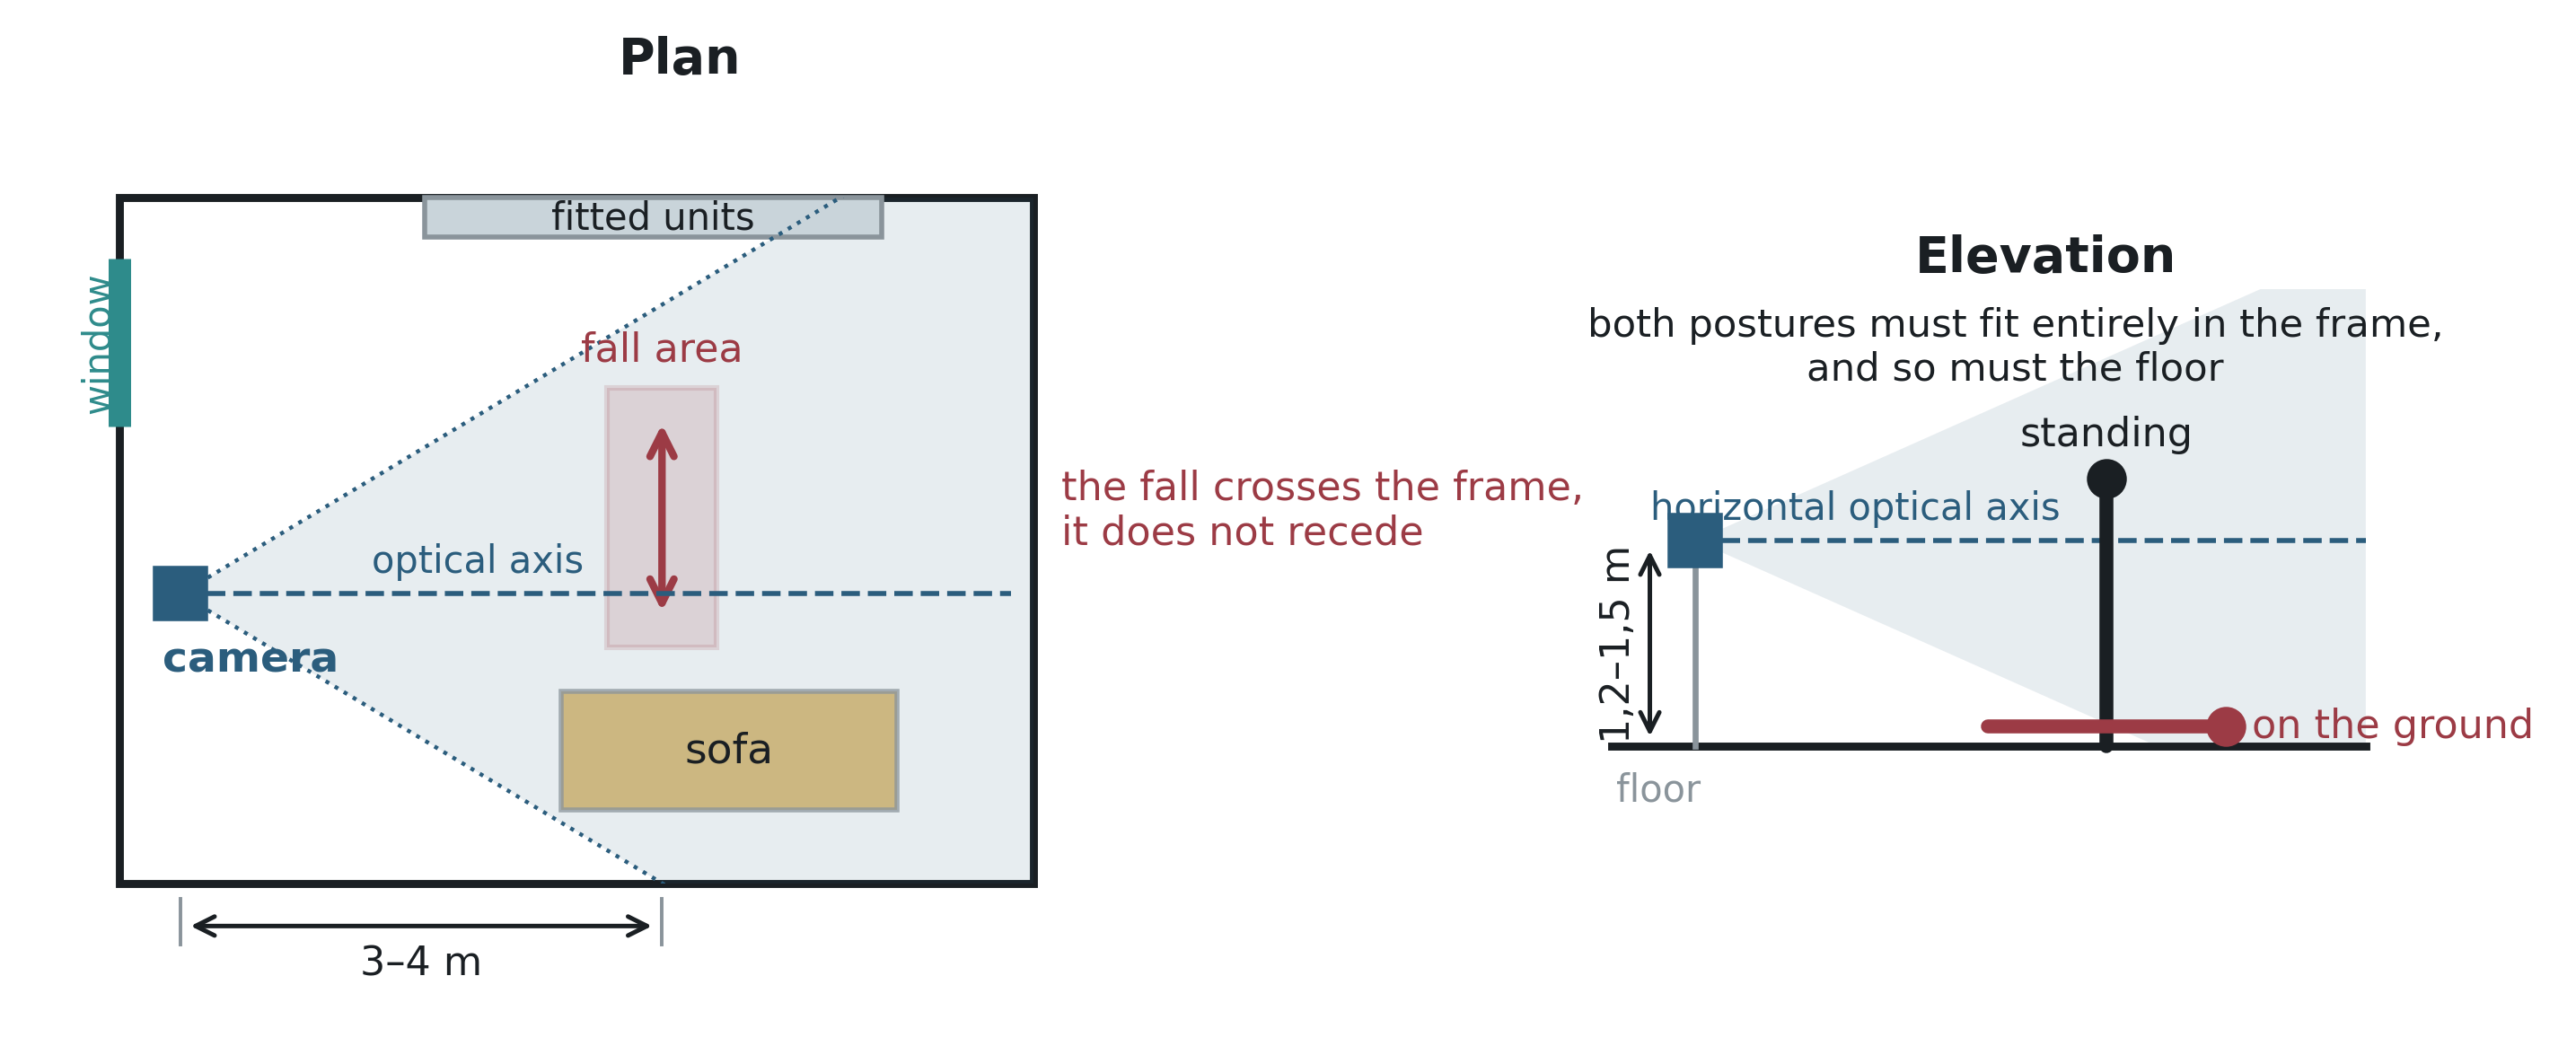
\includegraphics[width=0.85\textwidth]{figure/fig_stanza_en.png}
\caption{Layout scheme used during the domestic acquisitions.}
\label{fig:stanza}
\end{figure}

The system saves pose, features and classifier scores. The RGB images are retained locally only in the vicinity of the alerts, so that errors can be checked afterwards. The complete video stream is therefore neither transmitted nor stored continuously.

The acquisitions were carried out in real homes, with the lighting and the furnishings present in those environments and during ordinary daily activities.
The five falls considered in the first evaluation are all simulated. The elderly participants were not asked to perform falls; their recordings contain only ordinary daily activities, including situations in which the person remains lying on a sofa. These acquisitions therefore reproduce realistic domestic conditions, but do not constitute a clinical validation on natural falls.

\subsection{Quality of the acquisitions and usable data}

The continuous presence of people in the frame was not annotated. It is therefore not possible to measure directly the actual hours of people in the scene. What can be computed is the time during which the estimator returned a valid pose: 7,45~hours out of the 9,58 recorded, that is 77,8\%. This is a lower bound on the time of presence, because a person may be in the frame without producing a valid pose, for example when part of the body leaves the image.

\begin{table}[ht]
\centering
\caption{Share of frames with a valid pose across the days of acquisition.}
\label{tab:qualita_pose_domestiche}
\begin{tabular}{lll}
\toprule
\textbf{Day} & \textbf{Place} & \textbf{Valid poses} \\
\midrule
10 August & first home & 0,6--39,8\% \\
11 August & first home & 83,0\% \\
12 August & second home & 86,8--99,3\% \\
13 August & second home & 25,9--97,6\% \\
\bottomrule
\end{tabular}
\end{table}

The six blocks recorded on 10 August have a percentage of valid poses between 0,6\% and 39,8\%. The camera was too close and parts of the body often left the frame. These blocks are not used in the quantitative results that follow. On the following days the framing was widened.

\section{Event-level metrics}
\label{sec:falsi-allarmi}
\label{sec:finestre-eventi}

The classifier produces a probability for every temporal window. In continuous operation, however, several consecutive windows may exceed the threshold during the same fall or during the same activity. Treating every positive window as a new alarm would therefore overestimate the number of alerts received by the user. For this reason the decisions on the windows are kept distinct from the alarm events.

\subsection{From windows to alarm events}

The classifier produces a probability for every temporal window, but several consecutive windows may refer to the same activity. For this reason
we do not treat every window above the threshold as a new alarm, but
generate an alarm when at least five consecutive windows exceed the decision threshold.

After the alarm, a suspension interval of 30~s is applied, during which any subsequent positive windows are treated as part of the same episode.

The set used from here on comprises nine sessions, counted in wall-clock time: the eight blocks of the August campaign of Table~\ref{tab:protocollo_domestico} that exceed nine minutes, and the prolonged board session of 6 September. The four shortest August blocks, lasting between two and seven minutes, are excluded because a rate per hour computed on them would not be meaningful. The recordings were not all acquired with the same threshold: four of the nine sessions used $0{,}45$ and five used $0{,}50$.

Recomputing all the sessions with a threshold of $0{,}50$, the overall ratio between windows above the threshold and events changes by about 1\%. The difference therefore does not alter the conclusions, but it is kept explicit. Over the nine sessions used for this analysis, for a total duration of 14,98~hours, the ratio between windows above the threshold and events is 44,8.

\begin{figure}[htbp]
\centering
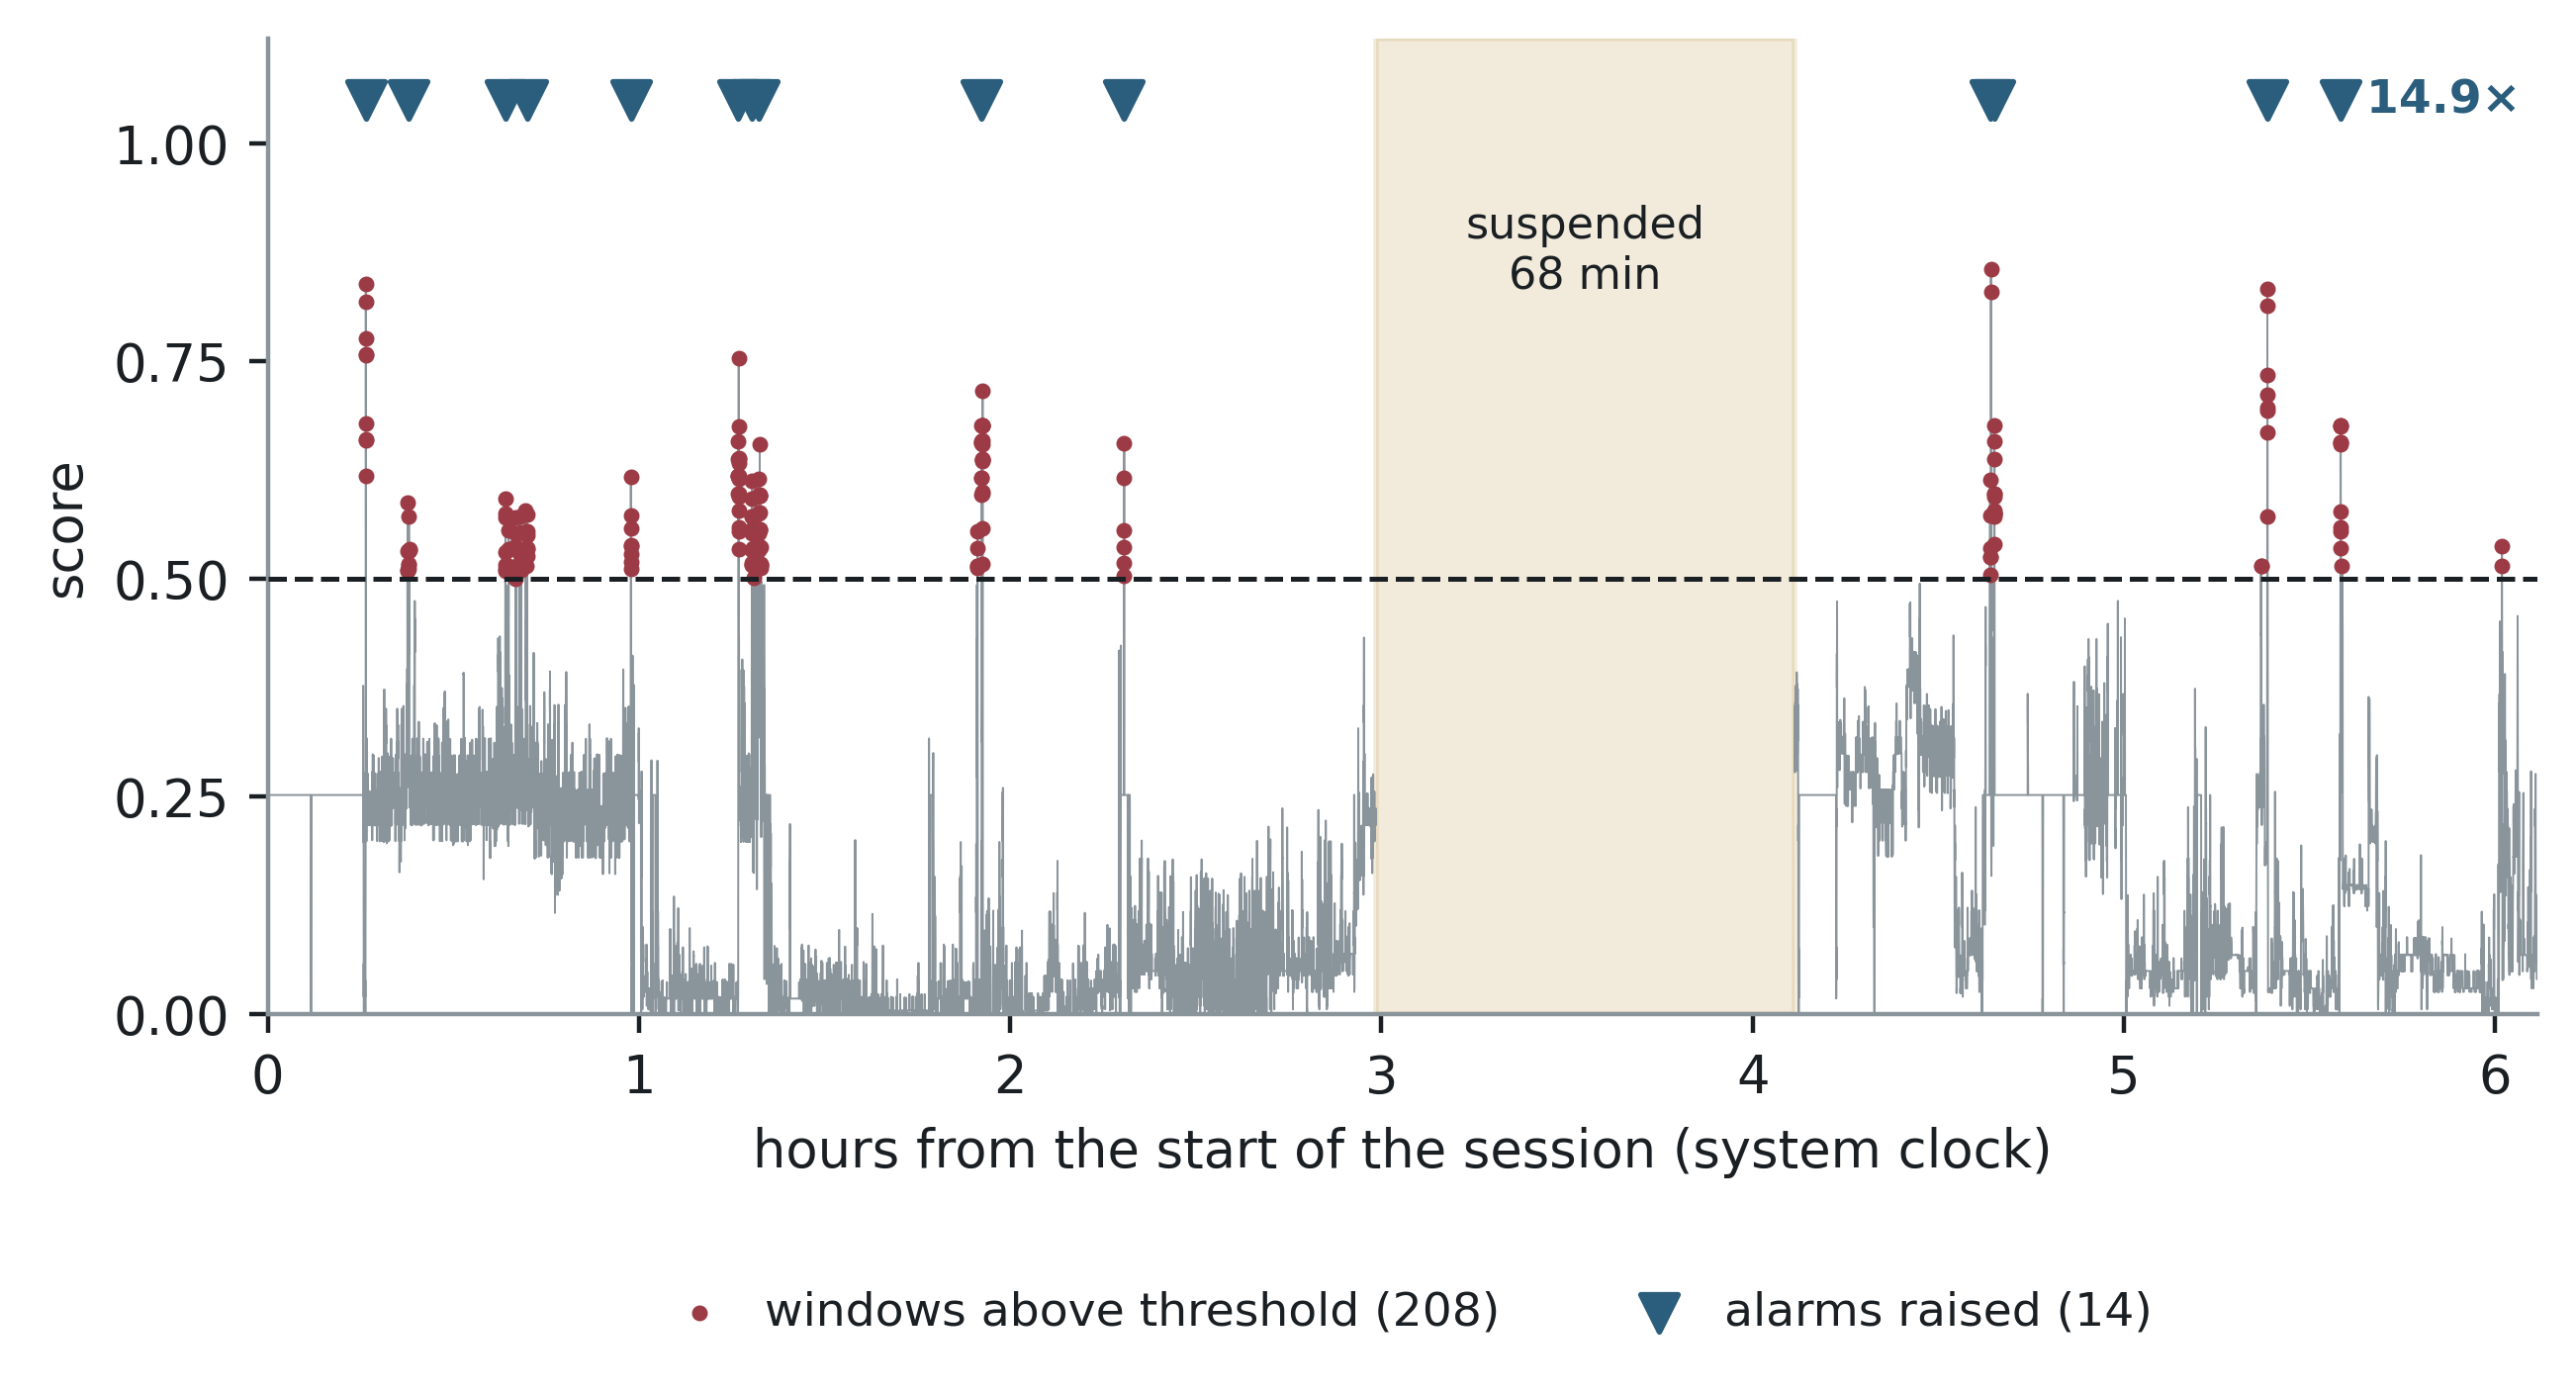
\includegraphics[width=0.85\textwidth]{figure/fig_sessione_en.png}
\caption{Positive windows and events generated during a prolonged session.}
\label{fig:sessione}
\end{figure}

In the session of 11 August shown in Figure~\ref{fig:sessione}, 208 windows above the threshold and 14 events generated are observed, a ratio of 14,9. The value differs from the overall ratio of 44,8 because the duration of the positive sequences changes from one recording to another. For the domestic trials the number of events per hour was therefore used as the main operational measure, keeping the number of windows above the threshold separate.

The latter remains useful for distinguishing a brief error from a persistent state. A person lying on a sofa, for example, may keep the score high for a prolonged period. The suspension interval reduces the number of alerts, but the classifier may go on interpreting that configuration as positive.

\subsection{Recall and criteria for associating the events}
\label{sec:recall-campo}

The five simulated falls were annotated only to the minute. In order to associate them with the alarms, the temporal tolerance and the persistence required were therefore varied.

\begin{table}[ht]
\centering
\caption{Falls associated with a detection as the criterion used varies.}
\label{tab:associazione_cadute}
\begin{tabular}{lcc}
\toprule
\textbf{Tolerance} &
\textbf{Persistence 1} &
\textbf{Persistence 5} \\
\midrule
$\pm10$ s & 0/5 & 0/5 \\
$\pm30$ s & 2/5 & 2/5 \\
$\pm60$ s & 4/5 & 2/5 \\
$\pm90$ s & 4/5 & 2/5 \\
\bottomrule
\end{tabular}
\end{table}

The result of 4/5 is obtained with a tolerance of $\pm60$~s and by treating a single positive window as sufficient. The first positive windows of the four falls recognised appear at $11{,}8$, $19{,}4$, $27{,}7$ and $32{,}3$~s from the annotated minute. The resulting recall is $0{,}80$, with a 95\% confidence interval running from $0{,}28$ to $0{,}99$. With only five falls the value is therefore very uncertain.

With the operational rule of five consecutive windows, by contrast, two of the five falls generate an event. The other three produce runs of two, three and zero positive windows, below the persistence threshold. Recall must therefore always be reported together with the association criterion used.

A difference was moreover found during this check between the offline analysis and the one carried out on the board. The first analysis indicated two falls recognised out of five, whereas during execution on the device four were obtained. The difference depended on two aspects. In the offline analysis the mean of the models obtained during cross-validation was used, whereas the model installed on the board was the final one, retrained on the whole set available. In addition, the subsampling from 18 to 9~fps was applied a second time to the board recordings. Once these two differences had been removed, the offline analysis reproduces the behaviour observed on the device.

A more precise check was possible in the session of 9 September, in which four simulated falls were annotated directly on the frames. The classifier recognises three of the four falls, while the aggregation rule generates two alarm events. Figures~\ref{fig:sessione_v5_andamento} and~\ref{fig:sessione_v5_cadute} show respectively the course of the whole session and the detail of the falls.

\begin{figure}[htbp]
\centering
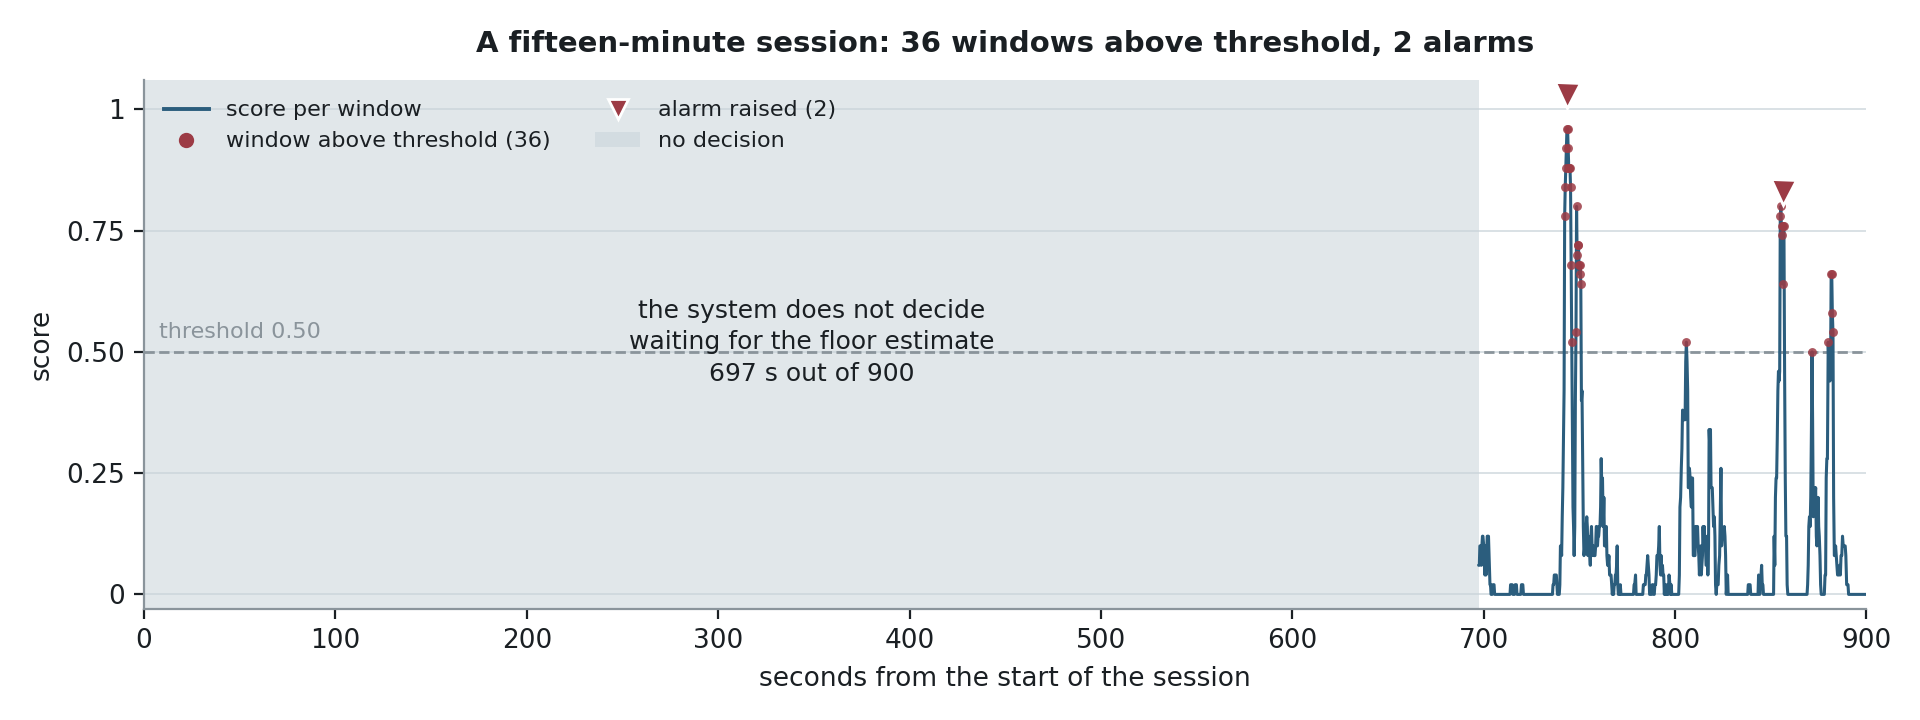
\includegraphics[width=.96\textwidth]{figure/fig_sessione_v5_andamento_en.png}
\caption{Course of the score during the session of 9 September. In the first 697~s the system produces no decisions, because the plane of the floor is not yet available. In the 203~s that follow, 624 windows are produced, 36 of them above the threshold, and two alarm events}
\label{fig:sessione_v5_andamento}
\end{figure}

\begin{figure}[htbp]
\centering
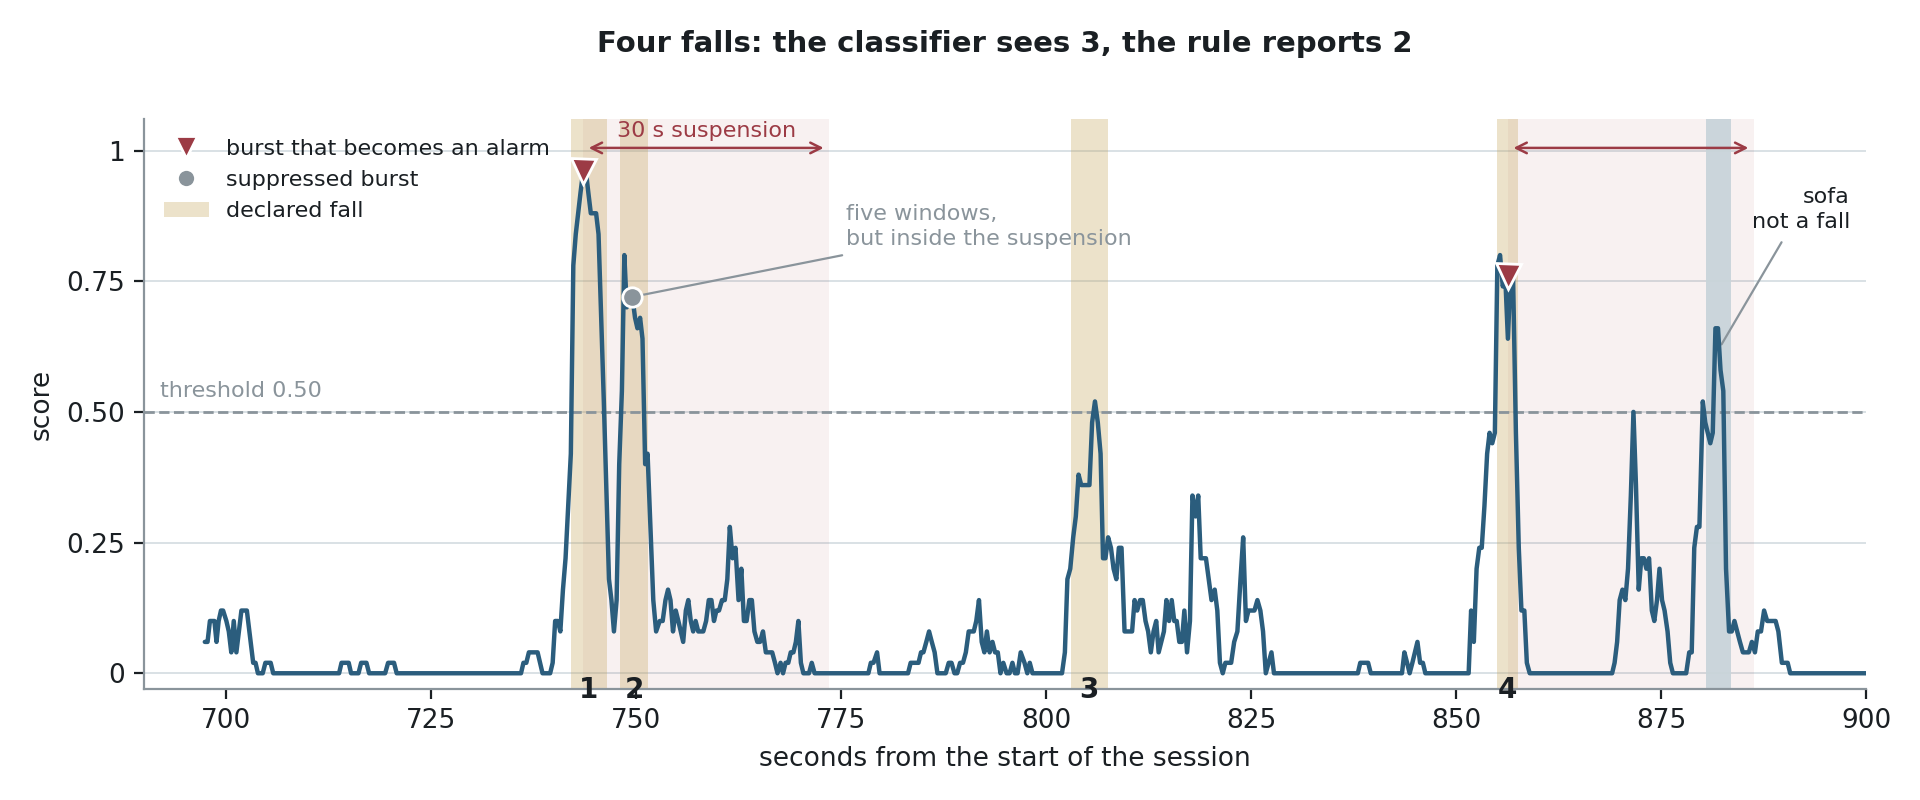
\includegraphics[width=.96\textwidth]{figure/fig_sessione_v5_cadute_en.png}
\caption{Detail of the four simulated falls and of the false positive associated with the sofa in the session of 9 September}
\label{fig:sessione_v5_cadute}
\end{figure}

The first fall produces a sufficient run of windows above the threshold and correctly generates an alarm. Figure~\ref{fig:caduta_board} shows a frame from the same sequence, with the skeleton and the score produced directly by the board.

\begin{figure}[htbp]
\centering
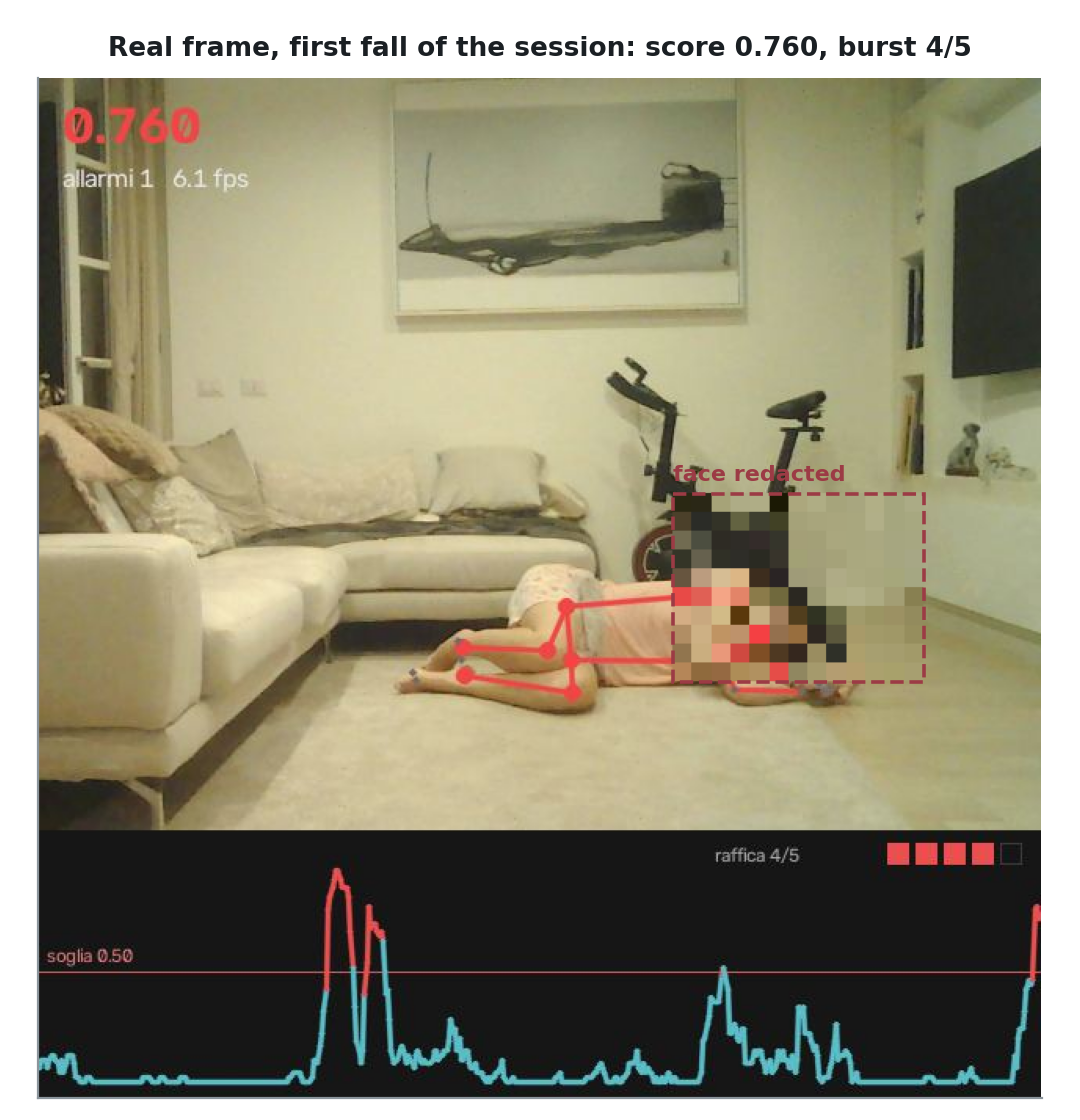
\includegraphics[width=0.75\textwidth]{figure/fig_caduta_board_en.png}
\caption{Real frame from the session of 9 September, with the skeleton and the score produced by the board. The overlay is the one the device draws in real time.}
\label{fig:caduta_board}
\end{figure}

The second fall occurs about six seconds after the first. The classifier recognises it, but no new alarm is generated because the system is still within the 30~s suspension interval. This case shows an important difference between an error of the classifier and an error of the aggregation logic: the fall was recognised by the model, but suppressed by the operational rule.

In the same session a person sitting on the sofa produces a run of four windows above the threshold. No alarm is generated, because the five consecutive windows required are not reached. Persistence therefore removes some false positives, but it can also suppress real events that are very close in time.

\subsection{Detection latency}
\label{sec:latenza}

Another important quantity is the latency, which ought to be measured between the beginning of the fall and the generation of the alarm. In the first domestic recordings this value cannot be obtained directly, because the falls are annotated only to the minute.

In the four falls recognised, the first positive window appears at 11,8, 19,4, 27,7 and 32,3~s respectively with respect to the annotated minute. These values do not, however, represent the latency of the system, because the exact second at which the fall began is not known.

What can be computed instead is the time introduced by the configuration of the pipeline. Considering a mean frequency of 8,02~fps, a window of 22 samples and a persistence of five consecutive windows, the following decomposition is obtained.

\begin{table}[ht]
\centering
\caption{Decomposition of the time introduced by the configuration of the pipeline at the mean frequency of 8,02~fps.}
\label{tab:latenza}
\begin{tabular}{lrr}
\toprule
\textbf{Component} & \textbf{Time} & \textbf{Share} \\
\midrule
Computation per frame & 0,125 s & 3,2\% \\
Filling of the window & 2,743 s & 71,0\% \\
Persistence & 0,997 s & 25,8\% \\
\midrule
Total & 3,865 s & 100\% \\
\bottomrule
\end{tabular}
\end{table}

The largest contribution is due to the filling of the window, 2,743~s. The computation per frame accounts for only 3,2\% of the total. Latency therefore depends above all on the length of the window and on the persistence required in order to generate the alarm. Reducing the processing time alone would have a smaller effect than changing these two parameters.

The value of 0,997~s represents the minimum time needed to obtain five consecutive windows. In the two falls for which the whole sequence is available, the time observed is instead 1,70 and 1,28~s. Some windows drop temporarily below the threshold, restarting the count.
With the annotations available it is therefore possible to estimate the time introduced by the pipeline, but not the full latency between the physical beginning of the fall and the alert.

\section{Comparison between benchmark and real behaviour}
\label{sec:rovesciamento}
\label{sec:confronto-domini}

Finally, the same configurations were compared on the benchmark and in the domestic recordings. The metrics used in the two cases are different, so the absolute values are not compared directly: what we observe is how the difference between the configurations changes in going from the dataset to the domestic environment.

\subsection{Comparison of the configurations}

Five configurations built on representation A3 were considered. A3h adds the height above the floor, A3i introduces the integral quantities, while the configurations with counter-examples also use negative examples collected in the domestic recordings.

The feature $h_{\text{pav}}$ had not been selected initially. It was reintroduced after false positives had been observed on people lying on raised surfaces. The result obtained on the same recordings is therefore not regarded as a verification independent of that choice.

\begin{table}[ht]
\centering
\caption{Comparison of the configurations on the benchmark and in the domestic recordings.}
\label{tab:configurazioni}
\begin{tabular}{lccc}
\toprule
\textbf{Configuration} &
\textbf{$F_2$ laboratory} &
\textbf{Windows/hour at home} &
\textbf{Falls} \\
\midrule
A3 & $0{,}898\pm0{,}075$ & 139,9 & 3/5 \\
A3h & $0{,}931\pm0{,}051$ & 70,4 & 2/5 \\
A3h + counter-examples & $0{,}942\pm0{,}060$ & 2,1 & 2/5 \\
A3i & $0{,}943\pm0{,}064$ & 9,8 & 4/5 \\
A3i + counter-examples & $0{,}953\pm0{,}055$ & 2,7 & 3/5 \\
\bottomrule
\end{tabular}
\end{table}

On the benchmark every configuration improves on A3. Between A3 and A3i with counter-examples the difference in $F_2$ is 0,055, of the same order as the variability between subjects. In the domestic recordings, by contrast, the positive windows went from 139,9 to 2,7 per hour, about 52 times fewer. The individual types of error also improve on the benchmark.

\begin{table}[ht]
\centering
\caption{False negatives and false positives of the five configurations in the LOSO evaluation on ten subjects.}
\label{tab:errori_configurazioni}
\begin{tabular}{lcccc}
\toprule
\textbf{Configuration} & \textbf{$F_2$} &
\textbf{Recall} & \textbf{FN} & \textbf{FP} \\
\midrule
A3 & 0,898 & 0,929 & 45 & 172 \\
A3h & 0,931 & 0,962 & 22 & 137 \\
A3h + counter-examples & 0,942 & 0,965 & 22 & 129 \\
A3i & 0,943 & 0,977 & 14 & 150 \\
A3i + counter-examples & 0,953 & 0,980 & 14 & 124 \\
\bottomrule
\end{tabular}
\end{table}

Going from A3 to A3i with counter-examples, the false negatives fall from 45 to 14 and the false positives from 172 to 124. The improvement in recall is therefore not obtained by increasing the false positives.

\subsection{Analysis of the differences between the two domains}

The main difference between the dataset and the domestic recordings concerns the negative activities with people in a horizontal position. In the dataset these activities take place mostly close to the floor. In the domestic recordings a person may instead be lying on a bed or a sofa.

\begin{table}[htbp]
\centering
\caption{Qualitative distribution of the negative configurations with a person in a horizontal position.}
\label{tab:negativi_orizzontali}
\begin{tabular}{lcc}
\toprule
\textbf{Domain} & \textbf{Approximate share} &
\textbf{Prevailing position} \\
\midrule
Laboratory & about a fifth & floor \\
Domestic environment & about half & raised surface \\
\bottomrule
\end{tabular}
\end{table}

The median height of the hips in the horizontal negatives is about $+0{,}02$ trunk lengths in the dataset and $+1{,}47$ in the domestic recordings.
This difference explains why $h_{\text{pav}}$ has a limited effect on the benchmark but turns out more useful in the domestic recordings. A benchmark can only assess the conditions present in its own data. If a situation typical of the real environment is poorly represented, a feature designed to distinguish it may have a reduced effect during the evaluation on the dataset.

\subsection{Transfer of the counter-examples}

The domestic counter-examples were collected in the same two homes used for the evaluation. In order to check whether the improvement depended on the individual room alone, the model was trained with the counter-examples of one home and evaluated in the other.

\begin{table}[ht]
\centering
\caption{Transfer of the counter-examples between the two homes.}
\label{tab:trasferimento_controesempi}
\begin{tabular}{lcc}
\toprule
\textbf{Counter-examples used} &
\textbf{Test home} &
\textbf{Events/hour} \\
\midrule
None / home 2 & home 1 & $0{,}342 \rightarrow 0{,}171$ \\
None / home 1 & home 2 & $1{,}781 \rightarrow 0{,}890$ \\
\bottomrule
\end{tabular}
\end{table}

In both cases the number of events per hour roughly halves. The improvement therefore does not depend on the room in which the examples were collected alone. With only two homes it is not, however, possible to verify generalisation to new environments. The counter-examples must therefore be regarded as a form of adaptation to the domestic domain. Moreover, with A3i, adding the counter-examples brings the falls recognised from 4/5 to 3/5. The same trade-off was observed when the three definitions of the task were compared.

\begin{table}[ht]
\centering
\caption{Behaviour of the three definitions of the task in the domestic recordings.}
\label{tab:compiti_domestici}
\begin{tabular}{lcc}
\toprule
\textbf{Task} & \textbf{Alarm events/hour} &
\textbf{Falls detected} \\
\midrule
Event & 1,6 & 3/5 \\
State & 29,5 & 0/5 \\
Alarm & 36,4 & 4/5 \\
\bottomrule
\end{tabular}
\end{table}

The \emph{event} task produces 1,6 events per hour, against 29,5 for the \emph{state} task and 36,4 for the \emph{alarm} task, but it recognises one fall fewer than the alarm task. Here too it is therefore not possible to evaluate a configuration by considering a single metric.

\begin{figure}[htbp]
\centering
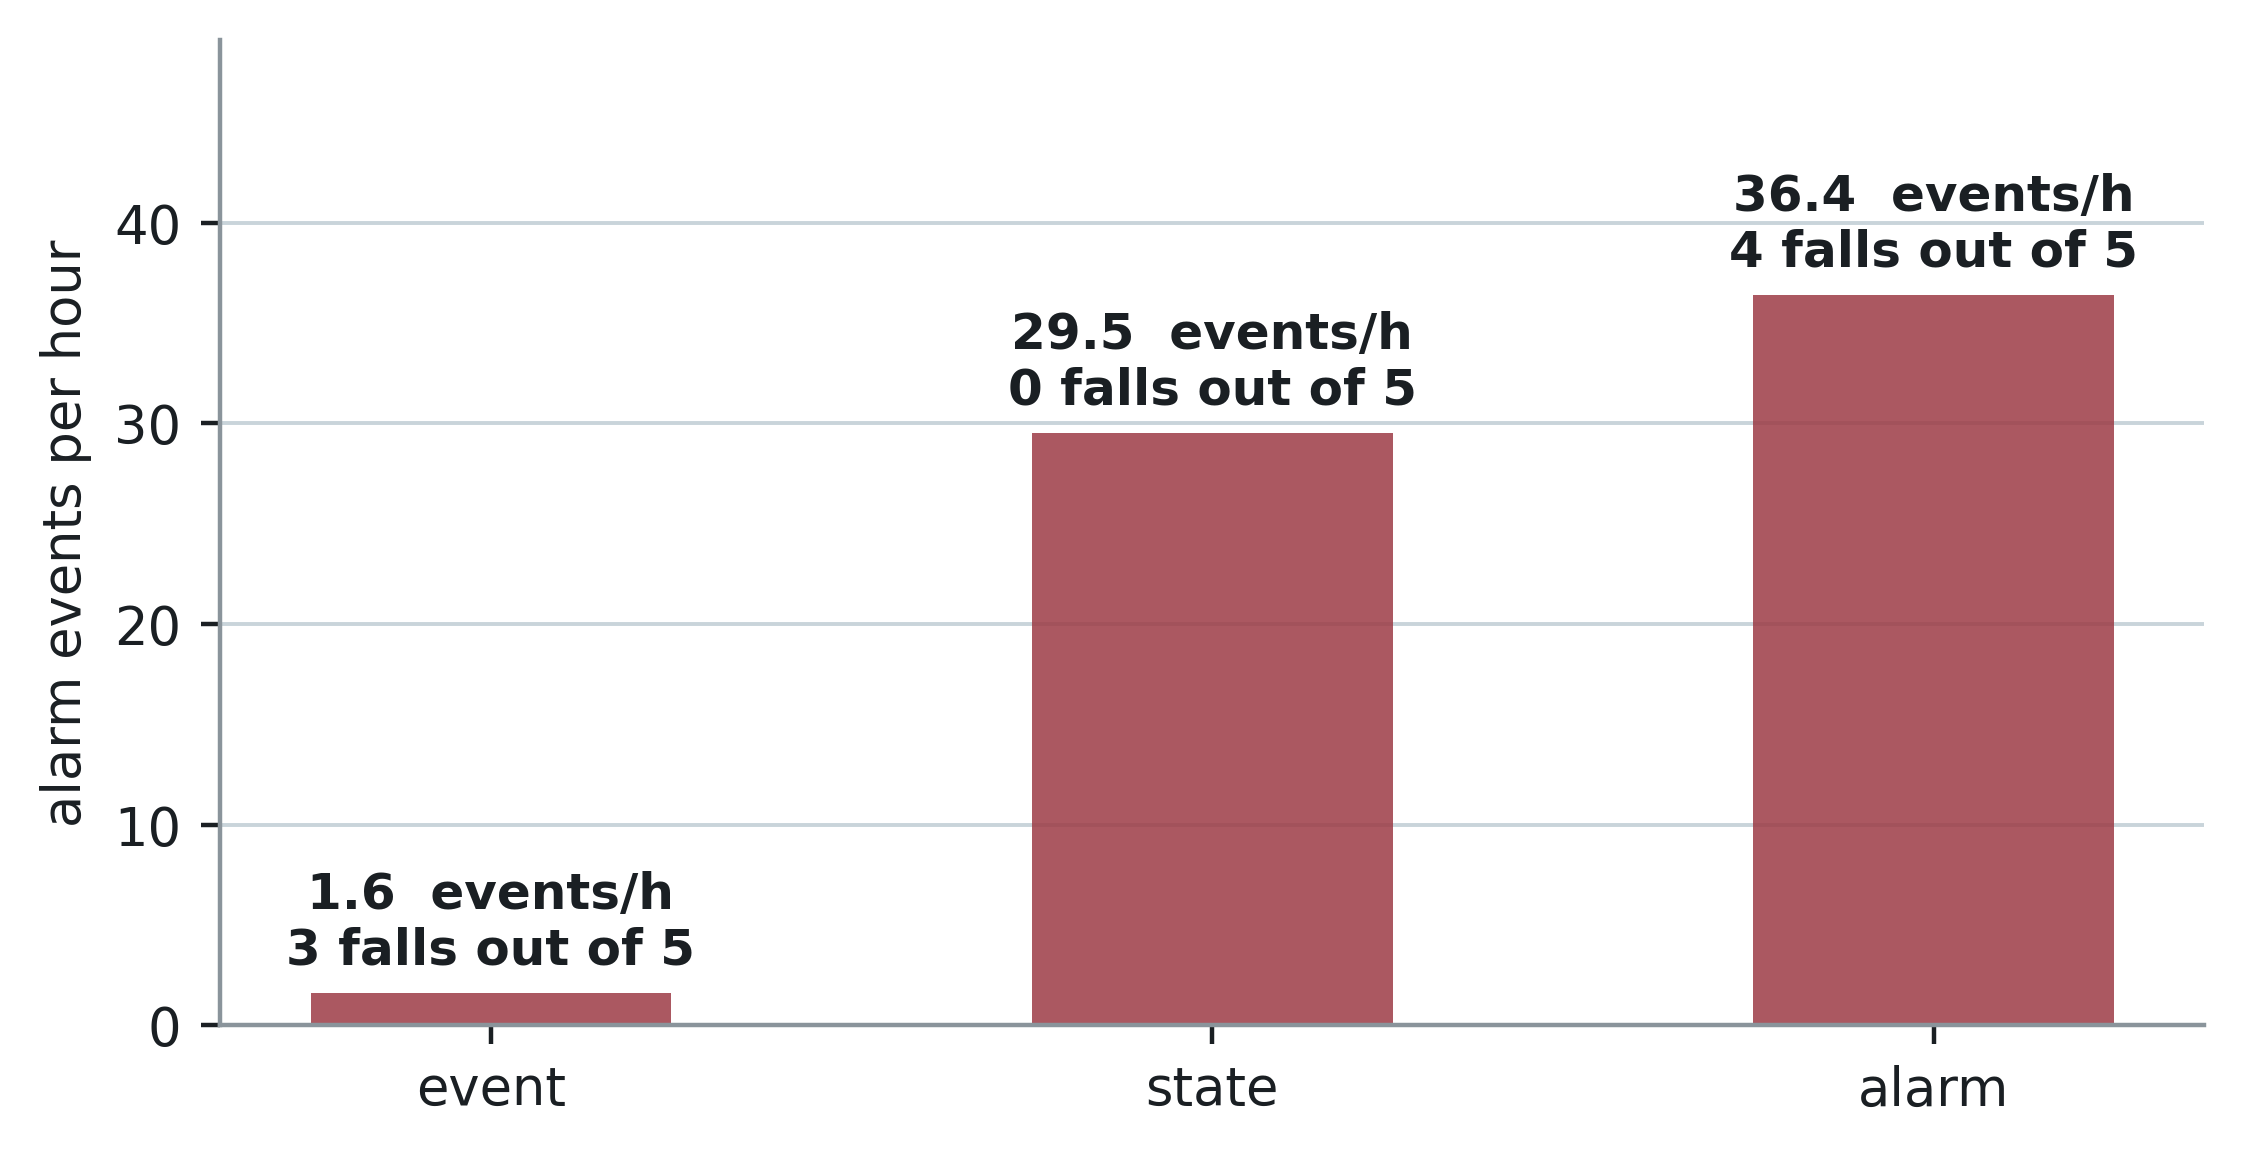
\includegraphics[width=.86\textwidth]{figure/fig_compiti_casa_en.png}
\caption{Comparison between the three definitions of the task in the domestic recordings, using the same event aggregation rule.}
\label{fig:compiti-casa}
\end{figure}

\subsection{Effect of the accumulation window}
\label{sec:finestra-k}

The integral quantities are computed over a sliding window of $K$ samples. Different values were tried while the rest of the pipeline was kept unchanged.
The laboratory results reported in Table~\ref{tab:effetto_k} come from the five-subject experiment and serve to describe the trend of the parameter.

\begin{table}[ht]
\centering
\caption{Effect of $K$ on the benchmark and in the domestic recordings.}
\label{tab:effetto_k}
\begin{tabular}{rrrrr}
\toprule
$K$ &
\textbf{$F_2$ laboratory} &
\textbf{FN} &
\textbf{Alarms/hour at home} &
\textbf{Falls} \\
\midrule
5  & $0{,}859\pm0{,}125$ & 23 & --    & -- \\
15 & $0{,}928\pm0{,}048$ & 24 & 137,6 & 4/5 \\
22 & $0{,}963\pm0{,}016$ & 9  & 17,3  & 4/5 \\
31 & $0{,}980\pm0{,}020$ & 4  & 14,0  & 4/5 \\
45 & $0{,}987\pm0{,}008$ & 3  & 17,0  & 3/5 \\
\bottomrule
\end{tabular}
\end{table}

On the benchmark, $F_2$ almost always increases as $K$ grows and reaches its maximum with $K=45$. At home, by contrast, going from $K=31$ to $K=45$ the alarms rise from 14,0 to 17,0 per hour and the falls recognised drop from 4/5 to 3/5.
The value $K=31$ was chosen partly on the basis of these domestic results. The choice is therefore not independent of the data used in the evaluation. Repeating the selection within the individual folds, nine folds out of ten choose $K=45$ and the mean $F_2$ increases by 0,026. If the laboratory result alone were used, $K=31$ would therefore not be chosen.

With $K=31$ the integral features use a longer history than the 22-sample window supplied to the classifier. The system remains causal, because only samples already observed are used and the accumulation is reset between independent recordings. $K$ does, however, represent a number of samples and not a fixed duration. At the median cadence of the archive, 31 samples correspond to about 1,72~s; across the recordings of the dataset the duration varies roughly between 1,58 and 2,15~s. On the device the misalignment is greater. At 9~fps, 31 samples correspond to about 3,4~s and, taking the classifier window into account as well, some features may depend on a total history of close to 5,8~s.

When the frequency of the board drops, the same number of samples covers an even longer interval. One solution for the future is to define $K$ as a duration and derive the number of samples from the actual frequency, instead of keeping it fixed.

\section{Failure modes and operational limitations}
\label{sec:fallimenti}
\label{sec:modi-fallire}

The domestic trials made it possible to observe some problems that do not emerge directly from the evaluation on the dataset. They concern both the representation used by the classifier and the prolonged operation of the device.

\subsection{Errors tied to the representation and to the scene}

The false positives on people lying down led us to check how far the score produced depended on the movement present in the window. The correlation measured is $+0{,}139$, therefore very low. The instantaneous derivatives moreover turned out to be sensitive to the noise of the pose and did not describe the dynamics in a stable way. From this observation the integral quantities used in configuration A3i were introduced.

A second problem concerns raised surfaces. In the negative frames with the person in a horizontal position, the median height of the hips is about $+0{,}02$ trunk lengths in the dataset and $+1{,}47$ in the domestic recordings. In the first case the person is generally close to the floor; in the second they may be lying on a bed or a sofa. This difference led to the reintroduction of $h_{\text{pav}}$ and to the use of the domestic counter-examples.

A geometric filter based on the trunk angle was also tested. With a threshold of $110^\circ$ the false positives drop from 141 to 65, but recall falls from 0,941 to 0,872 and the false negatives increase. The filter was therefore not retained in the final configuration.

\subsection{Presence of several people}

The pipeline was extended so as to keep the identity and the feature state of every person observed separate. In the only sequence available with
two people visible at the same time, made up of 291 frames, no
identity swaps were observed. The trial is, however, too short to validate multi-person tracking. UP-Fall, too, almost always contains a single person and cannot be used to check this case.

The presence of several people also increases the computational cost, because landmark estimation is carried out separately for each subject. In the trials, about 7,5~fps were measured with the room empty, 4~fps with one person and 2--3~fps with two. The reduction in frequency also changes the time interval represented by the windows. At 2--3~fps, 22 samples cover a much longer interval than the one used during training.

\subsection{Problems of continuous operation}
During one of the prolonged sessions the operating system suspended the board for about 68 minutes. The program remained active and resumed normally after the wake-up. A check between system time and monotonic time was therefore added in order to detect any interruptions.

We also observed the loss of the USB camera. In some cases the device is renumbered by the operating system, for example from \texttt{/dev/video0} to \texttt{/dev/video1}. The program may then remain active without receiving new frames. The camera is read in a separate thread and the main loop checks the time elapsed since the last frame. If it exceeds 20~s, the device is reopened. In the longest session this mechanism recovered capture in about twenty seconds; in an earlier trial the same problem had produced several minutes without images.

A further limitation concerns the computation of events per hour. Across the nine sessions considered, 1,41~hours without decisions are observed out of 14,98~total hours. Computing the rate only over the hours in which the system was actually producing decisions, the value goes from 11,1 to 12,2 events per hour, about 10\% more. The ratio between positive windows and events, 44,8, does not change, because both quantities are computed on the same decisions.

Taken together, the trials show that the pipeline can be run locally and kept active for prolonged periods, but they are not enough for the system to be regarded as validated for a real installation. The acquisitions concern only two homes and five simulated falls. Moreover, the session containing the five falls has a share of valid poses of 25,9\%, owing to sub-optimal framing. The recall values obtained in this part must therefore be read with these limitations in mind.


\chapter{Validazione in ambiente reale}
\label{cap:campo}

% ---------------------------------------------------------------------
% CAPITOLO NUOVO, non presente nella bozza iniziale.
% Nasce dalla richiesta esplicita del relatore di provare il sistema con
% una sessione lunga in una casa vera.
%
% Scritto il 2026-08-17, a sessioni eseguite. La sezione 6.2 contiene una
% previsione formulata PRIMA della prima sessione (EXP-032) e va letta
% come tale: e' il termine di paragone di tutto il capitolo.
%
% Fonti: EXP-032, EXP-036, EXP-043, EXP-044, EXP-047..EXP-054,
% ISS-036, ISS-040, ISS-042, docs/PROTOCOLLO_SESSIONE_REALE.md
% ---------------------------------------------------------------------

I capitoli precedenti hanno validato il sistema \emph{in vitro}: dieci soggetti, una stanza di laboratorio, cadute recitate su un materasso, annotazione fotogramma per fotogramma. Nessuna delle metriche prodotte finora dice cosa succede lasciando il sistema acceso per ore in una casa dove nessuno cade.

Questo capitolo risponde a quella domanda, e il risultato principale non è un numero di prestazione: è che \textbf{l'insieme di verifica su cui l'intero settore misura ordina in modo errato le alternative progettuali}.

\section{Perché il laboratorio non basta}
\label{sec:perche-non-basta}

Il divario fra prestazioni dichiarate e comportamento sul campo non è un'ipotesi di questo lavoro: è un fenomeno documentato. Bagalà e colleghi hanno preso tredici algoritmi di rilevamento cadute pubblicati, che dichiaravano sensibilità comprese fra il 76\% e il 100\% su cadute simulate, e li hanno rieseguiti su un archivio di ventinove cadute reali confermate. La sensibilità media misurata è stata del \textbf{57,0\%} con una dispersione di 27,3 punti, e i falsi allarmi in ventiquattro ore di monitoraggio andavano da cinque a ottantacinque al giorno a seconda dell'algoritmo.

Il fenomeno è stato riconfermato di recente e su scala molto maggiore. Il benchmark OmniFall unifica otto dataset pubblici di rilevamento cadute --- fra cui UP-Fall --- per circa ottanta ore annotate a livello di fotogramma, e li confronta con un insieme di cadute \emph{vere} riprese fuori dal laboratorio. Il modello addestrato su UP-Fall passa da un F1 di 72,9\% in dominio a \textbf{16,9\%} sulle cadute reali; su Le2i il crollo è da 100\% a 58,8\%. E il collo di bottiglia identificato è proprio la distinzione fra \emph{fallen} e \emph{lying}: i modelli confondono sistematicamente chi è caduto con chi è disteso.

Ci sono due ragioni per cui un dataset di laboratorio non può misurare ciò che serve, e sono di natura diversa.

La prima è la \textbf{frequenza di base}, ed è quantificabile a priori: è la sezione~\ref{sec:frequenza-base}.

La seconda è più insidiosa perché non si vede finché non si va a misurare: il dataset \textbf{non contiene le situazioni difficili} dell'ambiente di destinazione. UP-Fall non ha divani, non ha più persone in scena, e --- come si vedrà --- le sue persone orizzontali che non sono cadute stanno a terra invece che rialzate. Ogni intervento progettato per una condizione che il dataset non rappresenta viene giudicato da quel dataset come un peggioramento.

\section{Il problema della frequenza di base}
\label{sec:frequenza-base}

Questa sezione è stata scritta \emph{prima} della prima sessione, ed è importante che si legga in quest'ordine: contiene una previsione, e una previsione registrata dopo i fatti non è una previsione.

Il modello migliore del Capitolo~\ref{cap:risultati} produce circa 46 falsi positivi su 4.767 finestre negative, cioè lo \textbf{0,96\% per finestra}. In laboratorio, dove le finestre positive sono il 4,5\% del totale, quello 0,96\% corrisponde a una precision di 0,819 --- un numero che si presenta bene.

In un soggiorno la quota di finestre positive è circa lo zero per cento. Proiettando lo stesso tasso per finestra sul funzionamento continuo:

\begin{center}
\begin{tabular}{lrr}
\toprule
Modalità di finestratura & Finestre/giorno & Falsi allarmi/giorno \\
\midrule
Finestre non sovrapposte & $\sim$34.560 & $\sim$332 \\
Finestre con stride 5 & $\sim$311.000 & $\sim$2.990 \\
\bottomrule
\end{tabular}
\end{center}

Cioè fra \textbf{14 e 125 falsi allarmi all'ora}.

Il punto metodologico è che \textbf{la precision non è una proprietà del modello}: dipende da quanto sono frequenti gli eventi positivi nell'insieme su cui la si calcola. Riportare una precision misurata su un insieme quasi bilanciato come se descrivesse il comportamento in esercizio è un errore diffuso in letteratura, e qui viene quantificato con dati propri.

Il termine di paragone esterno rende la distanza esplicita. Il criterio che circola come soglia di accettabilità clinica è rilevare almeno il 95\% delle cadute con al massimo \textbf{uno o due falsi allarmi alla settimana}. I sistemi realmente installati e documentati riportano 73\% di sensibilità con un falso allarme ogni quarantasei giorni, oppure 80\% con uno ogni venti giorni --- e nel primo caso una precision del 37,5\%, in un sistema considerato funzionante. Fra la previsione di 14--125 allarmi all'ora e il bersaglio di uno o due alla settimana ci sono \textbf{tre o quattro ordini di grandezza}, e non si colmano migliorando il classificatore.

\section{Protocollo delle sessioni}
\label{sec:protocollo-campo}

Sono stati registrati \textbf{dodici blocchi in quattro giornate, in due abitazioni, per 9,6 ore complessive}. I partecipanti sono familiari dello studente, informati e consenzienti; il relatore è stato informato della natura della raccolta.

La telecamera è montata \textbf{lateralmente} a 1,5--2~m di altezza. Non è una scelta di comodo: discende direttamente dal risultato del Capitolo~\ref{cap:risultati}, dove il passaggio da una vista laterale a una frontale rialzata dimezza l'accuratezza.

I blocchi si dividono in tre tipi:

\begin{itemize}
  \item \textbf{vita normale}, che fornisce il denominatore dei falsi allarmi ed è l'unico tipo registrato a casa dei nonni;
  \item \textbf{cadute recitate}, con orari annotati dall'operatore, che fornisce il recall;
  \item \textbf{trappole}, cioè attività costruite per far sbagliare il sistema: sdraiarsi sul divano, sedersi di scatto, chinarsi, stare a terra volontariamente, più persone in campo.
\end{itemize}

\paragraph{Etica e privacy come contenuto, non come adempimento.} Il registratore scritto per queste sessioni salva in modo continuo \emph{soltanto posa e feature}: mai il video. Le immagini vengono conservate solo in una finestra di pochi secondi attorno agli allarmi, restano sul dispositivo e non entrano nel repository. È il \emph{privacy-by-design} argomentato nel Capitolo~\ref{cap:contesto} dimostrato in pratica invece che dichiarato --- e ha richiesto di rimuovere dal prototipo una registrazione video continua che era stata aggiunta per comodità di sviluppo e che contraddiceva l'argomento stesso della tesi.

Una scelta va dichiarata perché limita i risultati: \textbf{i partecipanti anziani non eseguono cadute recitate}. Nei loro blocchi c'è soltanto vita normale. La ragione è di sicurezza, e la conseguenza è che il recall non è mai misurato sulla popolazione a cui il sistema sarebbe destinato.

\section{La prima ora, e cosa ha cambiato}
\label{sec:prima-ora}

Il primo blocco è durato trentanove minuti e ha prodotto \textbf{2.735 allarmi all'ora}: \textbf{ventidue volte} il limite superiore della previsione della sezione~\ref{sec:frequenza-base}. Una previsione costruita per essere scomoda si è rivelata ottimistica di oltre un ordine di grandezza.

Il dato che spiega il meccanismo è la distribuzione nel tempo:

\begin{center}
\begin{tabular}{lrr}
\toprule
Minuti & Pose valide & Allarmi \\
\midrule
0--15 (stanza vuota) & 0--29\% & \textbf{0} \\
15--25 & 76\% & 105--124 \\
25--35 & 76--99\% & 454--462 \\
35--40 (cadute) & 81\% & 642 \\
\bottomrule
\end{tabular}
\end{center}

\textbf{Zero allarmi in quindici minuti di stanza vuota.} Il problema non è rumore di fondo: è che ogni movimento di una persona presente genera finestre positive, e a finestre sovrapposte un singolo evento ne produce decine.

\section{Falsi allarmi in funzionamento continuo}
\label{sec:falsi-allarmi}
\label{sec:finestre-eventi}

Nella sessione da cinque ore, dopo aver alzato la soglia, il tasso scende a 41,7 finestre sopra soglia all'ora, che diventano \textbf{3,41 allarmi all'ora contando gli eventi} invece delle singole finestre. È un miglioramento di quasi tre ordini di grandezza rispetto alla prima ora, ed è ancora un ordine di grandezza sopra gli 0,4 all'ora delle installazioni funzionanti documentate, e due o tre sopra il criterio clinico.

La terza sessione, a casa dei nonni, ha dato \textbf{1.635 allarmi all'ora}: \textbf{trentanove volte} la casa precedente, a parità di configurazione, di soglia e di stimatore. La causa è stata osservata direttamente sui fotogrammi conservati attorno agli allarmi: \textbf{due persone anziane distese su due divani, immobili, nel pomeriggio}. Non è un caso limite costruito per mettere in difficoltà il sistema; è la loro vita normale, ed è esattamente la popolazione a cui il sistema sarebbe destinato.

\paragraph{Il filtro temporale non basta, e la ragione è strutturale.} La logica di soppressione delle raffiche --- richiedere $N$ finestre consecutive sopra soglia e poi sospendere per un periodo --- è progettata per \emph{eventi}. Una persona distesa per un'ora non è un evento ma uno \emph{stato che dura}, e fa riscattare l'allarme a ogni scadenza del periodo di sospensione. Il filtro comprime le raffiche e non gli stati, e in una casa con anziani il falso positivo dominante è uno stato.

\subsection{Finestre contro eventi}

Prima di ogni altra cosa va fissata l'unità di misura, perché è all'origine di
gran parte dei numeri irriportabili di questo capitolo.

Il sistema produce una decisione ogni frazione di secondo. Una singola caduta
genera quindi una \emph{raffica} di finestre consecutive sopra soglia --- su
una delle sessioni registrate una sola caduta ne ha prodotte centoventinove ---
e contarle come altrettanti allarmi non è una semplificazione: è un errore di
un fattore misurato in \textbf{47,8}.

Un allarme è definito da due parametri dichiarati: \textbf{cinque finestre
consecutive} sopra soglia perché venga emesso, e \textbf{trenta secondi} di
sospensione dopo l'emissione. Ogni numero di questo capitolo espresso in
«eventi all'ora» adotta questa regola; i numeri espressi in «finestre all'ora»
la precedono, e i due non vanno confrontati fra loro né con la letteratura,
che riporta eventi.

\subsection{La definizione del compito, misurata in casa}

La diagnosi del paragrafo precedente --- il falso positivo dominante è uno
stato che dura, e nessun filtro temporale comprime uno stato --- contiene già
la soluzione, ma in una direzione che non è quella del filtro. Se lo stato è
il problema, il sistema non deve riconoscere lo stato.

I tre compiti definiti nel Capitolo~\ref{cap:metodologia} sono stati quindi
misurati sulle stesse registrazioni domestiche, con la stessa regola di
allarme e la stessa soglia:

\begin{center}
\begin{tabular}{lrr}
\toprule
Compito & Eventi/ora & Cadute rilevate \\
\midrule
\textbf{evento} --- la transizione & \textbf{1,6} & 3/5 \\
stato --- persona a terra & 29,5 & 0/5 \\
allarme --- l'uno o l'altro & 36,4 & 4/5 \\
\bottomrule
\end{tabular}
\end{center}

\textbf{Un fattore ventitré sui falsi allarmi, al costo di una caduta su
cinque.} Il compito \emph{stato}, che è la formulazione più diffusa in
letteratura, è anche l'unico che in queste registrazioni non rileva alcuna
caduta: riconosce la persona distesa sul divano e quella caduta a terra come
la stessa configurazione, e alla soglia dichiarata satura sui divani.

Il dato è coerente con quanto misurato in laboratorio nella
sezione~\ref{sec:compito-risultati}, dove il compito \emph{evento} sbaglia
sullo zero per cento delle finestre di persona distesa volontariamente. Che la
stessa scelta produca lo stesso ordine in due contesti così diversi è la
corroborazione più solida di cui questo lavoro disponga.

\paragraph{Che cosa questo \emph{non} risolve.} Un evento e mezzo all'ora resta
lontano dagli $0{,}05$ delle installazioni documentate, di un fattore trenta. E
il compito \emph{evento} paga il proprio vantaggio esattamente dove costa di
più: una caduta non rilevata su cinque. La direzione è giusta, la distanza dal
requisito clinico non è colmata.


\begin{figure}[ht]
\centering
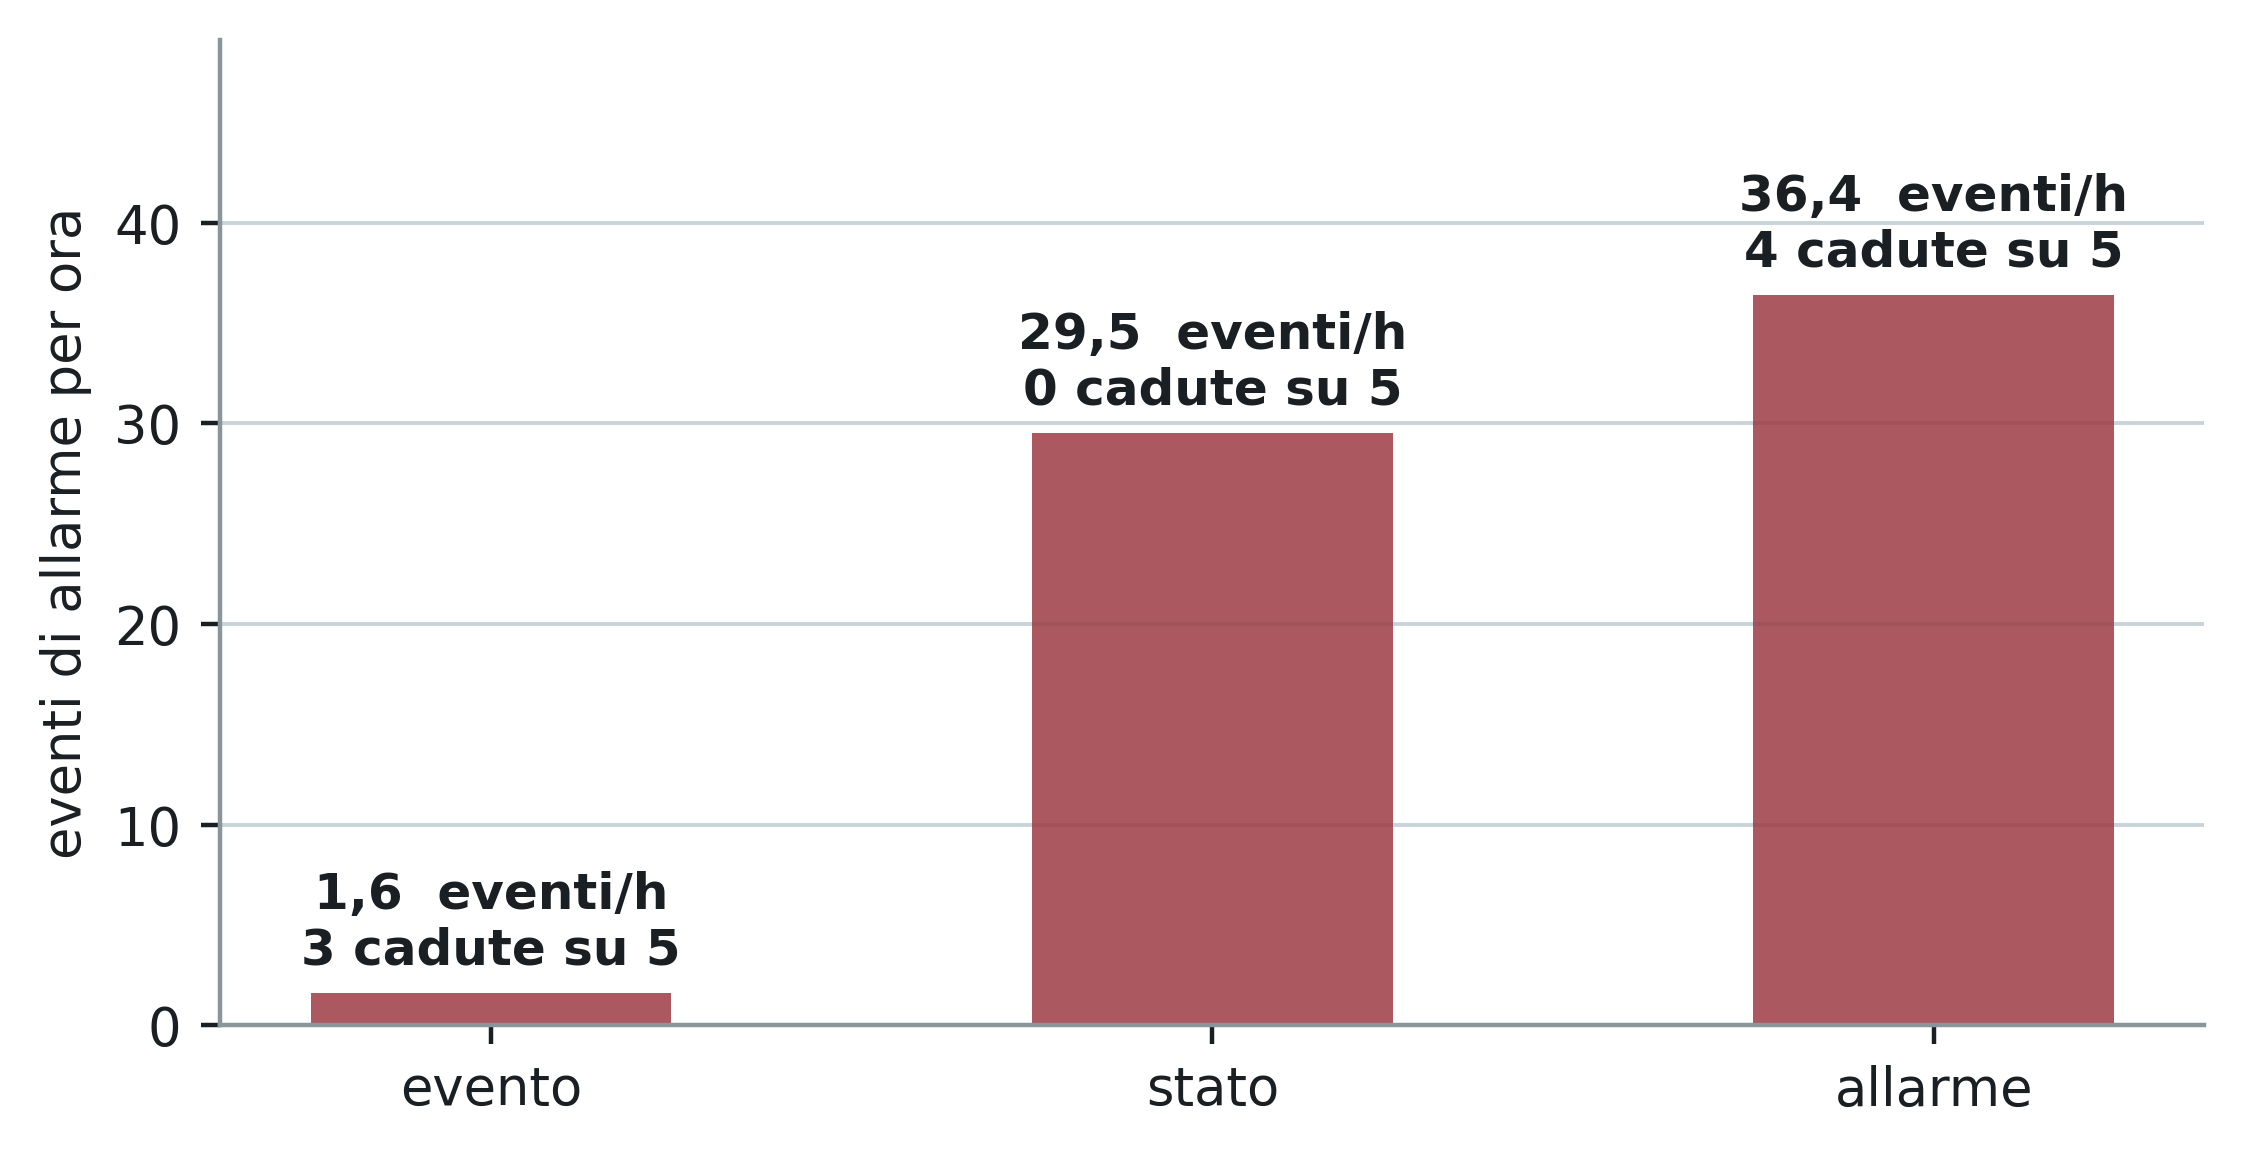
\includegraphics[width=.76\textwidth]{figure/fig_compiti_casa.png}
\caption{Gli stessi tre compiti misurati sulle registrazioni domestiche, con la regola di allarme dichiarata: cinque finestre consecutive sopra soglia e trenta secondi di sospensione. Il compito \emph{evento} è l'unico compatibile con un uso continuativo. Prodotta da \texttt{pipeline/figure\_tesi.py} sui risultati a dieci soggetti.}
\label{fig:compiti-casa}
\end{figure}

\section{Recall fuori dal laboratorio}
\label{sec:recall-campo}

Sulle cinque cadute annotate della sessione dedicata, la configurazione di riferimento ne rileva quattro.

Il numero va però letto con tre riserve, e la terza è emersa solo ricontando gli allarmi nel modo in cui li conterebbe chi usa il sistema.

La prima è la numerosità: \textbf{cinque cadute} non stimano un recall, danno un indizio. La seconda è che in quella sessione l'inquadratura era difettosa, con il corpo che esce dal bordo inferiore dell'immagine in quattro casi su cinque.

\paragraph{La terza: quel «quattro su cinque» conta finestre, non allarmi.} Un sistema installato non produce finestre ma \emph{eventi}: una caduta o viene segnalata o no, e una raffica di finestre consecutive sopra soglia è un allarme, non cento. Ricontando per evento, il recall dipende da due parametri dell'analisi che non erano stati dichiarati --- la \textbf{tolleranza di accoppiamento}, cioè entro quanto tempo dalla caduta annotata un allarme conta come rilevamento, e la \textbf{persistenza}, cioè quante finestre consecutive sopra soglia servono perché l'allarme scatti.

\begin{center}
\begin{tabular}{lcc}
\toprule
Tolleranza & Persistenza 1 & Persistenza 5 \\
\midrule
$\pm 10$~s & 0/4 & 0/4 \\
$\pm 30$~s & 2/5 & 1/5 \\
$\pm 60$~s & 3/5 & 1/5 \\
$\pm 90$~s & \textbf{4/5} & 1/5 \\
\bottomrule
\end{tabular}
\end{center}

Il valore riportato finora si colloca nell'angolo \emph{più permissivo} della tabella: una banda di tre minuti attorno alla caduta e un allarme che scatta su una singola finestra. Con parametri clinicamente difendibili --- l'allarme entro mezzo minuto e non su una finestra isolata --- il recall è \textbf{una caduta su cinque}.

La tolleranza larga non è sostenibile per due ragioni. L'annotazione dell'operatore è al minuto, quindi l'istante vero è noto a meno di sessanta secondi e $\pm 30$~s è già generoso; e in una sessione che produce centinaia di finestre sopra soglia all'ora, in una banda di tre minuti un allarme si trova quasi sempre, e viene attribuito alla caduta anche quando è stato causato da altro. Contraddice inoltre la motivazione clinica del Capitolo~\ref{cap:contesto}: se il danno dipende dal tempo passato a terra, un allarme novanta secondi dopo non è un rilevamento tempestivo.

Sullo stesso criterio è stato ricontato l'archivio esterno: su venti riprese di caduta di UR-Fall il sistema non ne segnala \textbf{nessuna}. Il conteggio per finestra ne dava nove su 144; per evento dà zero, perché i punteggi si fermano appena sotto la soglia e non vi restano abbastanza a lungo.

\paragraph{Il terzo parametro implicito.} È la terza volta in questo lavoro che un numero di intestazione dipende da un'impostazione dell'analisi lasciata come costante: dopo il sottocampionamento applicato alle sessioni e la media dei modelli della validazione incrociata al posto di quello installato, ora la tolleranza e la persistenza. Tutte e tre nella direzione che migliora il risultato, e nessuna per scelta deliberata --- sono impostazioni ereditate da uno script all'altro. Il rimedio adottato è esporle come parametri e riportare il recall di campo come \textbf{intervallo con i parametri dichiarati}, mai come numero singolo.

\paragraph{Un errore di misura che andava trovato prima di ogni confronto.} La valutazione fuori linea dava inizialmente 2 cadute su 5 dove la board, sugli stessi eventi e con lo stesso modello, ne aveva segnalate 4. Due procedure che guardano gli stessi dati non possono dare risultati diversi, e finché la discrepanza non è stata spiegata nessun confronto fra configurazioni era valido.

Le cause erano due. La prima, minore: fuori linea si mediavano i modelli della validazione incrociata, ciascuno addestrato su un sottoinsieme dei soggetti, mentre sul dispositivo gira un modello addestrato su tutti. La seconda, decisiva: l'analisi applicava alle sessioni lo stesso sottocampionamento usato su UP-Fall --- un fotogramma su due, per portare i 18~fps del dataset ai 9 su cui il modello è addestrato --- ma \textbf{le sessioni sulla board girano già a 7--8~fps}, e dimezzarle le porta a quattro. La finestra da 22 campioni copriva così cinque secondi e mezzo invece di due e mezzo, e la caduta ci si perdeva dentro.

È lo stesso difetto già trovato e risolto sul lato hardware, ricomparso \textbf{dal lato opposto della catena}: introdotto dall'analisi invece che dal dispositivo. Corrette entrambe le cause, la configurazione di riferimento dà 4 su 5, esattamente come la board.

\section{Che cosa il laboratorio non riesce a misurare}
\label{sec:rovesciamento}

È il risultato centrale del capitolo e, si sostiene qui, dell'intera tesi.

Tre interventi sono stati progettati per la robustezza in ambiente domestico:
l'altezza del bacino rispetto al pavimento stimata automaticamente
(\emph{A3h}); l'inserimento in addestramento di controesempi ricavati dalle
sessioni senza cadute; e le grandezze integrali al posto delle derivate
istantanee (\emph{A3i}). Tutti e tre sono stati valutati con la \emph{stessa}
procedura, sugli \emph{stessi} modelli, su due insiemi di verifica diversi:
la validazione incrociata su dieci soggetti di laboratorio, e sette ore di
registrazione continua in due abitazioni.

\begin{center}
\begin{tabular}{lrrr}
\toprule
Configurazione & $F_2$ laboratorio & Finestre/ora in casa & Cadute \\
\midrule
A3 --- riferimento & $0{,}898 \pm 0{,}075$ & 139,9 & 3/5 \\
A3h --- con l'altezza & $0{,}931 \pm 0{,}051$ & 70,4 & 2/5 \\
A3h + controesempi & $0{,}942 \pm 0{,}060$ & \textbf{2,1} & 2/5 \\
A3i --- con gli integrali & $0{,}943 \pm 0{,}064$ & 9,8 & \textbf{4/5} \\
\textbf{A3i + controesempi} & $\mathbf{0{,}953 \pm 0{,}055}$ & 2,7 & 3/5 \\
\bottomrule
\end{tabular}
\end{center}

\paragraph{Una precisazione sull'unità.} La colonna centrale conta
\textbf{finestre} sopra soglia per ora, non eventi di allarme. Le due
grandezze differiscono di quasi due ordini di grandezza, e la
sezione~\ref{sec:finestre-eventi} le distingue: qui si usano le finestre
perché è la grandezza su cui le cinque configurazioni sono direttamente
confrontabili, non perché sia quella da riportare.

\subsection{Le due graduatorie concordano. Non è questo il punto}

Va detto subito, perché una versione precedente di questo lavoro sosteneva il
contrario. Con cinque soggetti la configurazione A3h con i controesempi
risultava la \emph{peggiore} in laboratorio ($F_2 = 0{,}780$) e quasi la
migliore in casa, e se ne era tratto un rovesciamento dell'ordine. Con dieci
soggetti quella stessa configurazione ottiene $0{,}942$, e \textbf{le due
graduatorie non si contraddicono}: la configurazione peggiore in laboratorio è
anche la peggiore in casa.

Il rovesciamento era in larga parte un effetto della scarsità di dati. Averlo
scritto e poi smentito è, nell'economia di questo lavoro, un episodio della
stessa storia che il Capitolo~\ref{cap:protocollo} racconta: una differenza
più piccola della dispersione fra soggetti non è una differenza, e con cinque
persone $0{,}780$ e $0{,}917$ non lo erano.

\subsection{Il laboratorio non ordina male: non risolve}

La conclusione che sostituisce il rovesciamento si legge confrontando le due
colonne per \emph{ampiezza}, non per ordine.

\begin{center}
\begin{tabular}{lrr}
\toprule
Da A3 ad A3i + controesempi & In laboratorio & In casa \\
\midrule
Variazione & $+0{,}055$ di $F_2$ & da 139,9 a 2,7 finestre/ora \\
Rapporto & --- & \textbf{52$\times$} \\
Confronto con il rumore & \textbf{dentro} la dispersione ($\pm 0{,}06$--$0{,}08$) & --- \\
\bottomrule
\end{tabular}
\end{center}

\textbf{La stessa coppia di configurazioni differisce di un fattore
cinquantadue in una casa e di una quantità indistinguibile dal rumore in
laboratorio.} Il dataset di riferimento non sbaglia l'ordine: comprime una
differenza enorme in una differenza che non si può dichiarare.

L'effetto pratico è identico a quello di un ordinamento errato. Chi selezioni
la configurazione sulla base del solo $F_2$ di laboratorio non ha alcuna
ragione statistica per preferire A3i con i controesempi ad A3 di riferimento:
le due sono indistinguibili, e la seconda è più semplice. Sceglierebbe quindi
la più semplice, e installerebbe un sistema che produce cinquantadue volte i
falsi allarmi.

\subsection{La causa è misurabile, non congetturale}

In entrambi gli insiemi esistono persone orizzontali che non sono cadute, ma
sono di tipo opposto.

\begin{center}
\begin{tabular}{lrl}
\toprule
Negativi orizzontali & Quota & Dove stanno \\
\midrule
Archivio di laboratorio & circa un quinto & a terra \\
Sessioni domestiche & circa metà & su una superficie rialzata \\
\bottomrule
\end{tabular}
\end{center}

In laboratorio sdraiarsi sul pavimento è una delle azioni registrate come
attività ordinaria: lì «corpo a terra» non discrimina, perché a terra ci si
trova sia dopo una caduta sia per scelta. In una casa chi è orizzontale senza
essere caduto sta quasi sempre su un divano o su un letto, e la distinzione fra
divano e pavimento è esattamente quella che serve --- ed è quella che
l'archivio, non avendo divani, non può premiare.

Se ne ricava un enunciato che si ritiene valga oltre il caso particolare:

\begin{quote}
Un insieme di verifica non può misurare un miglioramento su una condizione che
non rappresenta. Non si limita a sovrastimare le prestazioni: \textbf{rende
indistinguibili alternative che in esercizio differiscono di ordini di
grandezza}, e lo fa con la stessa apparente sicurezza con cui distinguerebbe
alternative davvero equivalenti.
\end{quote}

\subsection{Il costo, che va dichiarato}

La tabella contiene anche il prezzo di questi interventi, e non è piccolo.

I controesempi domestici riducono le finestre in allarme di un fattore
cinquantadue, ma fanno scendere il recall da quattro cadute su cinque a tre. Su
A3h scendono a due. \textbf{Non è un miglioramento: è uno scambio}, e in un
sistema di sicurezza è lo scambio nella direzione che pesa di più.

C'è di più, ed è la riserva più seria del capitolo. I controesempi sono
ricavati dalle stesse abitazioni su cui il sistema viene poi misurato. La
verifica incrociata --- controesempi di una casa, misura sull'altra --- mostra
che il beneficio \emph{trasferisce}, ma dimezzato, e che il costo in recall
resta intero: da quattro cadute su cinque a due.

Il che significa che i controesempi sono \textbf{adattamento all'ambiente}, non
generalizzazione. Sono utili, e vanno raccolti al momento dell'installazione
come si tara un sensore; ma chiamarli robustezza sarebbe improprio, e due
abitazioni non bastano a dire quanto di quel beneficio sopravviva alla terza.

\section{Lo stesso fenomeno su un iperparametro}
\label{sec:finestra-k}

\paragraph{Provenienza di questa scansione.} I valori di laboratorio della
tabella provengono dall'impianto a \textbf{cinque} soggetti: la scansione non
è stata ripetuta su dieci, dove è stato misurato il solo $K = 31$ poi adottato.
La colonna di campo e il fenomeno che la sezione descrive non ne dipendono ---
riguardano il confronto fra due colonne, non il valore assoluto dell'una ---
ma i numeri di $F_2$ vanno letti come indicativi.


La compressione descritta nella sezione precedente riguarda scelte progettuali. Si ripresenta, in forma ancora più netta, su una singola costante numerica --- ed è stato trovato senza cercarlo, perché a quel punto ogni configurazione veniva misurata su entrambi gli insiemi.

Le grandezze integrali si accumulano su una finestra mobile di $K$ fotogrammi. Il valore iniziale, $K = 9$, era stato \emph{scelto} e non ottimizzato. Variandolo, con tutto il resto identico e con lo stesso $K$ usato anche nel calcolo sulle sessioni domestiche:

\begin{center}
\begin{tabular}{rrrrr}
\toprule
$K$ & F2 laboratorio & Falsi neg. & Falsi allarmi/ora & Cadute \\
\midrule
5 & $0{,}859 \pm 0{,}125$ & 23 & --- & --- \\
9 & $0{,}896 \pm 0{,}090$ & 21 & 156,7 & 4/5 \\
15 & $0{,}928 \pm 0{,}048$ & 24 & 137,6 & 4/5 \\
22 & $0{,}963 \pm 0{,}016$ & 9 & 17,3 & 4/5 \\
\textbf{31} & $\mathbf{0{,}980 \pm 0{,}020}$ & 4 & \textbf{14,0} & \textbf{4/5} \\
45 & $\mathbf{0{,}987 \pm 0{,}008}$ & \textbf{3} & 17,0 & \textbf{3/5} \\
\bottomrule
\end{tabular}
\end{center}

A $K = 31$ i falsi allarmi in casa scendono di un fattore undici a parità di recall, e la dispersione fra soggetti passa da $\pm 0{,}090$ a $\pm 0{,}020$.

La riga decisiva è l'ultima. Da $K = 31$ a $K = 45$ \textbf{l'F2 di laboratorio continua a salire} --- ed è il valore più alto misurato in tutto il lavoro --- \textbf{mentre sul campo si perde una caduta} e i falsi allarmi risalgono. Ottimizzando sulla sola metrica di laboratorio si sceglierebbe 45, cioè il valore sbagliato.

\paragraph{Perché non è un artefatto.} Per $K > 22$ la finestra di accumulazione supera quella di classificazione, quindi le grandezze integrali riassumono fotogrammi precedenti alla finestra su cui il modello decide. Va detto esplicitamente perché sembra sospetto, e non lo è: l'informazione è \emph{solo passata}, quindi disponibile in tempo reale a un sistema che riceve fotogrammi in streaming; le grandezze si calcolano da geometria e mai dalle etichette; l'accumulazione non attraversa il confine fra due riprese. La conferma sostanziale è che il miglioramento si osserva sulle \emph{sessioni domestiche}, che non entrano in alcuna validazione incrociata e che il modello non ha mai visto. Resta da dichiarare che il campo di ricezione temporale effettivo passa da 2,4~s a circa 5,8~s: il sistema decide su ventidue campioni, ma le sue feature riassumono più del doppio del tempo.

\section{I modi di fallire}
\label{sec:modi-fallire}

I blocchi costruiti per far sbagliare il sistema hanno prodotto tre risultati che vale la pena separare.

\paragraph{Il modello non guardava la dinamica.} L'obiezione naturale al problema del divano è che sdraiarsi e cadere hanno dinamiche diverse --- una lenta e controllata, l'altra rapida --- e che il modello dovrebbe distinguerle senza sapere dove si trova il corpo. La verifica ha mostrato che il modello assegnava punteggi alti anche a corpi completamente immobili, con una correlazione fra punteggio e movimento effettivo di $+0{,}139$: praticamente nulla. La causa non era il modello ma le grandezze fornite, ed è discussa nel Capitolo~\ref{cap:risultati}: le derivate istantanee hanno autocorrelazione a un fotogramma fra 0,11 e 0,41, contro 0,84--0,93 delle grandezze statiche. Ciò che arrivava al modello come dinamica era in gran parte rumore.

\paragraph{Il tracciamento multi-persona funziona e non è validabile.} È stato implementato con un'identità e un motore di feature indipendenti per ciascuna persona in scena. Nell'unica finestra in cui è stato messo alla prova --- 291 fotogrammi con due persone contemporaneamente visibili --- non ha prodotto alcuno scambio di soggetto. Ma nessuno degli archivi pubblici disponibili contiene più persone in scena: UP-Fall ne ha una sola nel 99,8\% dei fotogrammi. La capacità che serve davvero in una casa è precisamente quella che nessun dato di laboratorio può misurare, e settantun secondi di prova non la sostituiscono.

\paragraph{Un filtro geometrico in addestramento peggiora il bilancio.} Il \emph{Physics Guard} del prototipo iniziale agiva solo in inferenza. Portato anche in addestramento, con soglia a 110$^\circ$ sull'angolo del tronco, riduce i falsi positivi da 141 a 65 --- il valore più basso ottenuto senza controesempi --- ma porta il recall da 0,941 a 0,872 e raddoppia i falsi negativi. Con una metrica che pesa il recall il doppio della precision lo scambio è \textbf{netto negativo}, e i controesempi ottengono lo stesso effetto sui falsi positivi senza costare recall.

\section{Limiti operativi emersi sul campo}
\label{sec:limiti-operativi}

Due difetti non sarebbero emersi da nessuna misura di laboratorio, e sono parte del contributo di un capitolo sul funzionamento reale.

\paragraph{Il test che sembrava riuscito.} La prima sessione di durata terminava senza errori e con il registro completo fino in fondo. Il conteggio dei fotogrammi però non tornava con la durata dichiarata, e la temperatura della board era scesa di tredici gradi a metà sessione: \textbf{il dispositivo si era sospeso per inattività dopo venti minuti}, e il registratore, che misura il tempo con un orologio che durante la sospensione non avanza, non se ne era accorto. Il test non è fallito, \emph{è sembrato riuscire} --- che è il modo peggiore in cui una misura può essere sbagliata. La correzione è un secondo orologio, quello di sistema, con la differenza fra i due dichiarata nel riepilogo di ogni sessione.

\paragraph{Il frame rate crolla con il numero di persone.} Lo stimatore multi-persona esegue il modello dei punti corporei una volta per ciascuna persona rilevata. Con due persone in scena il sistema scende a 4~fps, e a quella frequenza la finestra temporale copre il doppio del tempo per cui il modello è stato addestrato. È lo stesso disallineamento fra frequenza di addestramento e di esercizio discusso nella sezione~\ref{sec:recall-campo}, qui indotto dall'hardware.

\section{Sintesi del capitolo}

Il sistema, nella configurazione ottimizzata, produce \textbf{14,0 falsi allarmi all'ora} contando le finestre sopra soglia, e ne rileva 4 su 5 con il criterio permissivo oppure 1 su 5 con quello clinicamente difendibile della sezione~\ref{sec:recall-campo}. Entrambi i valori restano sopra il criterio clinico di uno o due alla settimana, e questo va detto senza attenuazioni: il sistema misurato in questo lavoro \textbf{non è pronto per l'installazione}.

Ma il capitolo non serviva a dimostrare che lo fosse. Serviva a misurare la distanza, a spiegarne il meccanismo, e a mostrare che \textbf{quella distanza non è visibile dall'insieme di verifica su cui il settore misura} --- il quale, anzi, avrebbe indicato la direzione opposta.


% ---------------------------------------------------------------
% \clearpage prima di \addcontentsline: senza, la voce dell'indice
% prende il numero della pagina corrente, che e' l'ultima del
% capitolo precedente, e non quella su cui \include fa cominciare la
% bibliografia. Errore di una pagina, su entrambe le voci.
%
% I nomi dei file rispettano le maiuscole: Overleaf compila su Linux,
% dove \include{bibliografia} non trova Bibliografia.tex.
% ---------------------------------------------------------------
\clearpage
\phantomsection
\addcontentsline{toc}{chapter}{Bibliography}
\markboth{Bibliografia}{Bibliografia}
\begin{thebibliography}{99}

\bibitem{BA} F. Bagalà, C. Becker, A. Cappello, L. Chiari, K. Aminian,
J. M. Hausdorff, W. Zijlstra, and J. Klenk, {\it Evaluation of Accelerometer-Based Fall Detection Algorithms on Real-World Falls}, PLOS ONE, {\bf 7}(5) (2012).

\bibitem{BL} V. Bazarevsky, I. Grishchenko, K. Raveendran, T. Zhu, F. Zhang, and M. Grundmann, {\it BlazePose: On-device Real-time Body Pose tracking}, CVPR Workshop on Computer Vision for Augmented and Virtual Reality, 2020.

\bibitem{BR} R. W. Broadley, J. Klenk, S. B. Thies, L. P. J. Kenney, and M. H. Granat, {\it Methods for the Real-World Evaluation of Fall Detection Technology:
A Scoping Review}, Sensors, {\bf 18}(7) (2018), 2060.

\bibitem{DILL2024} S. Dill, A. Ahmadi, M. Grimmer, D. Haufe, M. Rohr,
Y. Zhao, M. Sharbafi, C. Hoog Antink, {\it Accuracy Evaluation of 3D Pose
Reconstruction Algorithms Through Stereo Camera Information Fusion for
Physical Exercises with MediaPipe Pose}, Sensors, {\bf 24}(23) (2024), 7772.

\bibitem{FN} Federazione Nazionale degli Ordini delle Professioni
Infermieristiche (FNOPI), {\it Allarme ISTAT su invecchiamento popolazione:
infermieri decisivi per il futuro del Paese}, comunicato del 1 settembre 2026.

\bibitem{SK} M. Feng, J. Meunier, {\it Skeleton Graph-Neural-Network-Based
Human Action Recognition: A Survey}, Sensors, {\bf 22}(6) (2022), 2091.

\bibitem{GU} J. Gutiérrez, V. Rodríguez, and S. Martin, {\it Comprehensive Review of Vision-Based Fall Detection Systems}, Sensors, {\bf 21}(3) (2021), 947.

\bibitem{HO} V.-H. Hoang, J. W. Lee, M. J. Piran, C.-S. Park, {\it Advances in
Skeleton-Based Fall Detection in RGB Videos: From Handcrafted to Deep
Learning Approaches}, IEEE Access, {\bf 11} (2023), 92322--92352.

\bibitem{IS} Istituto Nazionale di Statistica (ISTAT), {\it Rapporto
annuale 2026. La situazione del Paese}, Roma, maggio 2026.

\bibitem{PA} Istituto Superiore di Sanità, {\it Sorveglianza PASSI d'Argento: una caduta nell'ultimo anno per 1 anziano su 5}, biennio 2023--2024.

\bibitem{KR} M. Kangas, I. Vikman, L. Nyberg, R. Korpelainen,
J. Lindblom, T. J\"ams\"a, {\it Comparison of real-life accidental falls in
older people with experimental falls in middle-aged test subjects}, Gait \&
Posture, {\bf 35}(3) (2012), 500--505.

\bibitem{KA} M. Kangas, R. Korpelainen, I. Vikman, L. Nyberg, and T. Jämsä,
\textit{Sensitivity and False Alarm Rate of a Fall Sensor in Long-Term Fall
Detection in the Elderly}, Gerontology, {\bf 61} (2015), 61--68.

\bibitem{RL} R. Li, H. Fu, W. L. Lo, Z. Chi, Z. Song, D. Wen, {\it
Skeleton-Based Action Recognition With Key-Segment Descriptor and Temporal
Step Matrix Model}, IEEE Access, {\bf 7} (2019), 169782--169795.

\bibitem{LN} C.-B. Lin, Z. Dong, W.-K. Kuan, Y.-F. Huang, {\it A Framework for
Fall Detection Based on OpenPose Skeleton and LSTM/GRU Models}, Applied
Sciences, {\bf 11}(1) (2021), 329.

\bibitem{LI} J. Liu, X. Li, S. Huang, R. Chao, Z. Cao, S. Wang, A. Wang,
L. Liu, {\it A review of wearable sensors based fall-related recognition
systems}, Engineering Applications of Artificial Intelligence, {\bf 121}
(2023), 105993.

\bibitem{MP} C. Lugaresi, J. Tang, H. Nash, C. McClanahan, E. Uboweja,
M. Hays, F. Zhang, C.-L. Chang, M. Yong, J. Lee, W.-T. Chang, W. Hua,
M. Georg, M. Grundmann, {\it MediaPipe: A Framework for Building Perception
Pipelines}, 2019.

\bibitem{MV} L. Mart\'inez-Villase\~nor, H. Ponce, J. Brieva, E. Moya-Albor,
J. N\'u\~nez-Mart\'inez, and C. Pe\~nafort-Asturiano, {\it UP-Fall Detection Dataset: A Multimodal Approach}, Sensors, {\bf 19}(9) (2019), 1988.

\bibitem{MU} M. Mubashir, L. Shao, L. Seed, {\it A survey on fall
detection: Principles and approaches}, Neurocomputing, {\bf 100} (2013),
144--152.

\bibitem{NIE3D} B. X. Nie, P. Wei, S.-C. Zhu, {\it Monocular 3D Human Pose
Estimation by Predicting Depth on Joints}, in Proceedings of the IEEE
International Conference on Computer Vision (ICCV), 2017, 3467--3475.

\bibitem{RA}
H. Rahmani and M. Bennamoun,
Learning Action Recognition Model From Depth and Skeleton Videos,
Proceedings of the IEEE International Conference on Computer Vision (ICCV),
pp. 5832--5841, 2017.

\bibitem{SA} S. Samanta, B. Chanda, {\it A Data-driven Approach for
Human Pose Tracking Based on Spatio-temporal Pictorial Structure},
arXiv:1608.00199, 2016.

\bibitem{AM} S. Scheurer, J. Koch, M. Kucera, H. Bryn, M. B\"artschi,
T. Meerstetter, T. Nef, P. Urwyler, {\it Optimization and Technical Validation
of the AIDE-MOI Fall Detection Algorithm in a Real-Life Setting with Older
Adults}, Sensors, {\bf 19}(6) (2019), 1357.

\bibitem{SC} S. Scheurer, S. Tedesco, B. O'Flynn, and K. N. Brown,
{\it Comparing Person-Specific and Independent Models on Subject-Dependent
and Independent Human Activity Recognition Performance}, Sensors, {\bf 20}(13)
(2020), 3647.

\bibitem{SN} D. Schneider, Z. Marinov, M. Mistol, Z. Zhong, A. Jaus,
R. D\"uger, R. Baur, M. S. Sarfraz, R. Stiefelhagen, {\it OmniFall: From Staged
Through Synthetic to Wild --- A Unified Multi-Domain Dataset for Robust Fall
Detection}, arXiv:2505.19889, 2025.

\bibitem{WA} X. Wang et al., {\it A Real-time skeleton-based fall
detection algorithm based on temporal convolutional networks and
transformer encoder}, Pervasive and Mobile Computing, 2025.

\bibitem{ZH} X. Zhang, X. Wang, X. Fan, {\it Bridging the visual-to-physical
gap: physically aligned representations for fall risk analysis}, Frontiers
in Medicine, {\bf 13} (2026), art. 1837781.

\end{thebibliography}





 






\clearpage
\phantomsection
\addcontentsline{toc}{chapter}{Acknowledgements}
\chapter*{Acknowledgements}
\markboth{Acknowledgements}{Acknowledgements}

I would like to dedicate these last lines to the people who have been beside me during this journey and who, in one way or another, have helped me to reach this important goal.

First of all, I would like to thank my supervisor, Alessandro Mecocci, for his availability, his patience and the valuable advice he gave me during the work and the writing of this thesis.

My greatest thanks go to my family, who have been close to me throughout this whole journey and who have never let me go without their support. Thank you for believing in me, for respecting my choices and for giving me the chance to study and to reach this goal with peace of mind.

Thanks to my boyfriend Niccolò, who over these years has been close to me in the most difficult moments. Thank you for listening to me, encouraging me and helping me not to give up when I thought I could not make it, and for putting up with all my moments of stress during this journey.

Finally, I would like to thank the friends I have met during these last years at university, with whom I have shared lectures, exams and many days spent together, and my lifelong friends, who continue to be part of my life.


\end{document}
